%---------------------------------------------------------------------%
\documentclass[a4paper,11pt]{book}
%\documentclass[a4paper,12pt]{report}
%---------------------------------------------------------------------%
% MODIFY TEXT APPEARANCE
%---------------------------------------------------------------------%
% \usepackage[default]{comicneue}

%\usepackage[sfdefault]{FiraSans} %% option 'sfdefault' activates Fira Sans as the default text font
%\renewcommand*\oldstylenums[1]{{\firaoldstyle #1}}
%\renewcommand{\familydefault}{\sfdefault}

\usepackage[light,math]{iwona}
\renewcommand{\sldefault}{it} % In headers, automatically replace \textsl (which doesn't exist for iwona) by \textit

\newcommand{\deriv}{\mathrm{d}}
\newcommand{\Deriv}{\mathrm{D}}
\newcommand{\Rayleigh}{\mathrm{Ra}}
\newcommand{\Prandtl}{\mathrm{Pr}}
\newcommand{\Nusselt}{\mathrm{Nu}}
\newcommand{\Reynolds}{\mathrm{Re}}
\newcommand{\Grashof}{\mathrm{Gr}}
\newcommand{\Peclet}{\mathrm{Pe}}
\newcommand{\COP}{\mathrm{COP}}

\newcommand{\RE}{\mathfrak{Re}}
\newcommand{\IM}{\mathfrak{Im}}
%\newcommand{\RE}{\mathrm{Re}}
%\newcommand{\IM}{\mathrm{Im}}

\usepackage[utf8]{inputenc}
\usepackage[T1]{fontenc}
\emergencystretch=1em
%\let\epsilon\varepsilon
%\let\phi\varphi
\let\textss\textsuperscript

\usepackage{layout}
\renewcommand{\thesubparagraph}{\theparagraph.\roman{subparagraph}}
\renewcommand{\theparagraph}{\thesubsubsection.\alph{paragraph}}
\renewcommand{\thechapter}{\Roman{chapter}}
\renewcommand{\thesection}{\thechapter.\arabic{section}}
\renewcommand{\thesubsection}{\thesection.\arabic{subsection}}


\newcommand{\echaf}[1]{\textcolor{red}{\{?#1?\}}}
%---------------------------------------------------------------------%
% PACKAGES
%---------------------------------------------------------------------
\newcommand{\mylocaltoc}{
	\vfill
	\hrule \vspace{.5cm}
	{\hypersetup{linkcolor = black}
		\localtableofcontents
	}%
	\vspace{.5cm} \hrule
	\vfill
	\clearpage
}

\usepackage[french]{babel}
\usepackage{csquotes}
\usepackage{wrapfig}
\usepackage{comment}
\usepackage{multicol}
\usepackage{array}
	\newcolumntype{L}[1]{>{\raggedright\let\newline\\\arraybackslash\hspace{0pt}}m{#1}}
	\newcolumntype{C}[1]{>{\centering\let\newline\\\arraybackslash\hspace{0pt}}m{#1}}
	\newcolumntype{R}[1]{>{\raggedleft\let\newline\\\arraybackslash\hspace{0pt}}m{#1}}
	\setlength{\extrarowheight}{5pt}
\usepackage{longtable}
\usepackage{arydshln}
	\setlength\dashlinedash{1pt}
	\setlength\dashlinegap{1.5pt}
%	\setlength\arrayrulewidth{1cm}
\usepackage{tabularray}
	
%\newcommand{\mycite}[4]{
%	\begin{flushright}
%	\begin{tabular}{R{#4}L{#4}}
%		\multicolumn{2}{r}{#1}\\
%		\textit{-- #2} & \textbf{#3}
%	\end{tabular}
%\end{flushright}
%}
\usepackage{float}
% -----------------------------------------------------
\usepackage[dvipsnames]{xcolor}
	\definecolor{PythonBlue}{HTML}{1f77b4}
	\definecolor{PythonOrange}{HTML}{ff7f0e}
	\definecolor{PythonGreen}{HTML}{2ca02c}
	\definecolor{PythonRed}{HTML}{d62728}
	\definecolor{PythonPurple}{HTML}{9467bd}
	\definecolor{PythonBrown}{HTML}{8c564b}
	\definecolor{PythonPink}{HTML}{e377c2}
	\definecolor{PythonGray}{HTML}{7f7f7f}
	\definecolor{PythonOlive}{HTML}{bcbd22}
	\definecolor{PythonCyan}{HTML}{17becf}
	%----------------------------------
	\definecolor{MatlabBlue}{rgb}{0, 0.4470, 0.7410}
	\definecolor{MatlabDeepBlue}{HTML}{00375c}
	\definecolor{MatlabOrange}{rgb}{0.8500, 0.3250, 0.0980}
	\definecolor{MatlabDeepOrange}{HTML}{69280c}
	\definecolor{MatlabYellow}{rgb}{0.9290, 0.6940, 0.1250}
	\definecolor{MatlabDeepYellow}{HTML}{7a5a0b}
	\definecolor{MatlabPurple}{rgb}{0.4940, 0.1840, 0.5560}
	\definecolor{MatlabGreen}{rgb}{0.4660 ,0.6740 ,0.1880}
	\definecolor{MatlabCyan}{rgb}{0.3010, 0.7450, 0.9330}
	\definecolor{MatlabBrown}{rgb}{0.6350, 0.0780, 0.1840}
	% %----------------------------------
	\definecolor{Blue1}{HTML}{330099}%{030164} %
	\definecolor{Blue2}{HTML}{000099}%{050296}
	\definecolor{Blue3}{HTML}{003399}%{0603c8}
	\definecolor{Blue4}{HTML}{6600ff}%{0804fa}
	\definecolor{Blue5}{HTML}{0000ff}%{3936fb}
	\definecolor{Blue6}{HTML}{0066ff}%{6b68fc}

	\definecolor{Cyan1}{HTML}{0099cc}%{004a66} %
	\definecolor{Cyan2}{HTML}{009999}%{006f99}
	\definecolor{Cyan3}{HTML}{339999}%{0094cc}
	\definecolor{Cyan4}{HTML}{00ddff}%{00b9ff}
	\definecolor{Cyan5}{HTML}{00dddd}%{33c7ff}
	\definecolor{Cyan6}{HTML}{66dddd}%{66d5ff}

	\definecolor{Green1}{HTML}{009966}%{006600} %
	\definecolor{Green2}{HTML}{009900}%{009900}
	\definecolor{Green3}{HTML}{669900}%{00cc00}
	\definecolor{Green4}{HTML}{00ffcc}%{00ff00}
	\definecolor{Green5}{HTML}{00ff00}%{33ff33}
	\definecolor{Green6}{HTML}{ccff00}%{66ff66}

	\definecolor{Yellow1}{HTML}{b56727}%{656600} %
	\definecolor{Yellow2}{HTML}{be5504}%{999900}
	\definecolor{Yellow3}{HTML}{fc6a03}%{cbcc00}
	\definecolor{Yellow4}{HTML}{e5c000}%{feff00}
	\definecolor{Yellow5}{HTML}{ffe600}%{feff33}
	\definecolor{Yellow6}{HTML}{f6e683}%{feff66}
	
	\definecolor{Red1}{HTML}{990033}%{660000} %
	\definecolor{Red2}{HTML}{990000}%{990000}
	\definecolor{Red3}{HTML}{993300}%{cc0000}
	\definecolor{Red4}{HTML}{ff0066}%{ff0000}
	\definecolor{Red5}{HTML}{ff0000}%{ff3333}
	\definecolor{Red6}{HTML}{ff6600}%{ff6666}
	%----------------------------------
	\definecolor{ju0}{HTML}{000000}
	\definecolor{ju1}{HTML}{2d0377}
	\definecolor{ju2}{HTML}{7e03a8}
	\definecolor{ju3}{HTML}{b52f8c}
	\definecolor{ju4}{HTML}{de5f65}
	\definecolor{ju5}{HTML}{f89540}
	\definecolor{ju6}{HTML}{fbd524}
	\definecolor{ju7}{HTML}{f0f921}
	%----------------------------------
	\definecolor{PlasmaBlue}{HTML}{0C0786}
	\definecolor{PlasmaViolet}{RGB}{168,34,150}
	\definecolor{PlasmaPink}{HTML}{CA4678}
	\definecolor{PlasmaOrange}{RGB}{247,147,65}
	\definecolor{PlasmaYellow}{HTML}{EFF821}
	%----------------------------------
	\definecolor{Plasma1}{RGB}{12,7,135}
\definecolor{Plasma2}{RGB}{19,6,137}
\definecolor{Plasma3}{RGB}{27,6,141}
\definecolor{Plasma4}{RGB}{31,5,143}
\definecolor{Plasma5}{RGB}{38,5,146}
\definecolor{Plasma6}{RGB}{42,5,147}
\definecolor{Plasma7}{RGB}{47,4,150}
\definecolor{Plasma8}{RGB}{53,4,152}
\definecolor{Plasma9}{RGB}{56,4,154}
\definecolor{Plasma10}{RGB}{61,3,156}
\definecolor{Plasma11}{RGB}{65,3,157}
\definecolor{Plasma12}{RGB}{70,3,159}
\definecolor{Plasma13}{RGB}{73,2,160}
\definecolor{Plasma14}{RGB}{78,2,162}
\definecolor{Plasma15}{RGB}{83,1,163}
\definecolor{Plasma16}{RGB}{86,1,164}
\definecolor{Plasma17}{RGB}{91,0,165}
\definecolor{Plasma18}{RGB}{94,0,166}
\definecolor{Plasma19}{RGB}{99,0,167}
\definecolor{Plasma20}{RGB}{102,0,167}
\definecolor{Plasma21}{RGB}{106,0,168}
\definecolor{Plasma22}{RGB}{111,0,168}
\definecolor{Plasma23}{RGB}{114,0,169}
\definecolor{Plasma24}{RGB}{119,1,168}
\definecolor{Plasma25}{RGB}{122,1,168}
\definecolor{Plasma26}{RGB}{126,3,168}
\definecolor{Plasma27}{RGB}{129,4,167}
\definecolor{Plasma28}{RGB}{134,6,167}
\definecolor{Plasma29}{RGB}{138,8,166}
\definecolor{Plasma30}{RGB}{141,11,165}
\definecolor{Plasma31}{RGB}{145,14,163}
\definecolor{Plasma32}{RGB}{148,16,162}
\definecolor{Plasma33}{RGB}{152,19,160}
\definecolor{Plasma34}{RGB}{156,23,158}
\definecolor{Plasma35}{RGB}{158,25,157}
\definecolor{Plasma36}{RGB}{162,28,154}
\definecolor{Plasma37}{RGB}{165,30,153}
\definecolor{Plasma38}{RGB}{169,34,150}
\definecolor{Plasma39}{RGB}{171,36,149}
\definecolor{Plasma40}{RGB}{175,40,146}
\definecolor{Plasma41}{RGB}{178,43,143}
\definecolor{Plasma42}{RGB}{180,45,141}
\definecolor{Plasma43}{RGB}{184,49,138}
\definecolor{Plasma44}{RGB}{186,51,137}
\definecolor{Plasma45}{RGB}{189,54,134}
\definecolor{Plasma46}{RGB}{191,57,132}
\definecolor{Plasma47}{RGB}{194,60,129}
\definecolor{Plasma48}{RGB}{197,63,126}
\definecolor{Plasma49}{RGB}{199,66,124}
\definecolor{Plasma50}{RGB}{202,69,122}
\definecolor{Plasma51}{RGB}{204,71,120}
\definecolor{Plasma52}{RGB}{207,75,117}
\definecolor{Plasma53}{RGB}{208,77,115}
\definecolor{Plasma54}{RGB}{211,80,112}
\definecolor{Plasma55}{RGB}{214,84,110}
\definecolor{Plasma56}{RGB}{215,86,108}
\definecolor{Plasma57}{RGB}{218,89,105}
\definecolor{Plasma58}{RGB}{220,92,104}
\definecolor{Plasma59}{RGB}{222,95,101}
\definecolor{Plasma60}{RGB}{224,98,99}
\definecolor{Plasma61}{RGB}{226,101,97}
\definecolor{Plasma62}{RGB}{228,105,94}
\definecolor{Plasma63}{RGB}{230,107,92}
\definecolor{Plasma64}{RGB}{232,111,90}
\definecolor{Plasma65}{RGB}{233,113,88}
\definecolor{Plasma66}{RGB}{235,117,86}
\definecolor{Plasma67}{RGB}{237,121,83}
\definecolor{Plasma68}{RGB}{238,123,81}
\definecolor{Plasma69}{RGB}{240,127,79}
\definecolor{Plasma70}{RGB}{241,129,77}
\definecolor{Plasma71}{RGB}{243,133,74}
\definecolor{Plasma72}{RGB}{244,136,73}
\definecolor{Plasma73}{RGB}{246,140,70}
\definecolor{Plasma74}{RGB}{247,144,67}
\definecolor{Plasma75}{RGB}{248,147,66}
\definecolor{Plasma76}{RGB}{249,151,63}
\definecolor{Plasma77}{RGB}{250,154,61}
\definecolor{Plasma78}{RGB}{251,158,59}
\definecolor{Plasma79}{RGB}{251,161,57}
\definecolor{Plasma80}{RGB}{252,165,54}
\definecolor{Plasma81}{RGB}{253,169,52}
\definecolor{Plasma82}{RGB}{253,172,50}
\definecolor{Plasma83}{RGB}{254,177,48}
\definecolor{Plasma84}{RGB}{254,180,46}
\definecolor{Plasma85}{RGB}{254,185,44}
\definecolor{Plasma86}{RGB}{254,188,43}
\definecolor{Plasma87}{RGB}{254,192,41}
\definecolor{Plasma88}{RGB}{254,197,39}
\definecolor{Plasma89}{RGB}{253,200,38}
\definecolor{Plasma90}{RGB}{253,205,37}
\definecolor{Plasma91}{RGB}{252,208,36}
\definecolor{Plasma92}{RGB}{251,213,36}
\definecolor{Plasma93}{RGB}{251,217,36}
\definecolor{Plasma94}{RGB}{249,222,36}
\definecolor{Plasma95}{RGB}{248,227,37}
\definecolor{Plasma96}{RGB}{247,230,37}
\definecolor{Plasma97}{RGB}{245,235,38}
\definecolor{Plasma98}{RGB}{244,239,39}
\definecolor{Plasma99}{RGB}{242,244,38}
\definecolor{Plasma100}{RGB}{240,249,33}

	\definecolor{Inferno1}{RGB}{0,0,3}
\definecolor{Inferno2}{RGB}{0,0,6}
\definecolor{Inferno3}{RGB}{1,1,11}
\definecolor{Inferno4}{RGB}{2,2,16}
\definecolor{Inferno5}{RGB}{4,3,22}
\definecolor{Inferno6}{RGB}{6,4,27}
\definecolor{Inferno7}{RGB}{9,6,33}
\definecolor{Inferno8}{RGB}{13,8,40}
\definecolor{Inferno9}{RGB}{15,9,45}
\definecolor{Inferno10}{RGB}{19,10,52}
\definecolor{Inferno11}{RGB}{22,11,57}
\definecolor{Inferno12}{RGB}{26,12,64}
\definecolor{Inferno13}{RGB}{29,12,69}
\definecolor{Inferno14}{RGB}{34,11,76}
\definecolor{Inferno15}{RGB}{39,11,83}
\definecolor{Inferno16}{RGB}{43,10,87}
\definecolor{Inferno17}{RGB}{48,10,92}
\definecolor{Inferno18}{RGB}{52,9,95}
\definecolor{Inferno19}{RGB}{57,9,99}
\definecolor{Inferno20}{RGB}{60,9,101}
\definecolor{Inferno21}{RGB}{66,9,104}
\definecolor{Inferno22}{RGB}{71,10,106}
\definecolor{Inferno23}{RGB}{74,11,107}
\definecolor{Inferno24}{RGB}{79,13,108}
\definecolor{Inferno25}{RGB}{82,14,109}
\definecolor{Inferno26}{RGB}{87,15,109}
\definecolor{Inferno27}{RGB}{90,17,110}
\definecolor{Inferno28}{RGB}{95,18,110}
\definecolor{Inferno29}{RGB}{100,20,110}
\definecolor{Inferno30}{RGB}{103,21,110}
\definecolor{Inferno31}{RGB}{108,23,110}
\definecolor{Inferno32}{RGB}{111,24,110}
\definecolor{Inferno33}{RGB}{116,26,110}
\definecolor{Inferno34}{RGB}{120,28,109}
\definecolor{Inferno35}{RGB}{124,29,109}
\definecolor{Inferno36}{RGB}{128,31,108}
\definecolor{Inferno37}{RGB}{132,32,107}
\definecolor{Inferno38}{RGB}{136,33,106}
\definecolor{Inferno39}{RGB}{140,35,105}
\definecolor{Inferno40}{RGB}{144,36,104}
\definecolor{Inferno41}{RGB}{149,38,103}
\definecolor{Inferno42}{RGB}{152,39,101}
\definecolor{Inferno43}{RGB}{157,41,100}
\definecolor{Inferno44}{RGB}{160,42,98}
\definecolor{Inferno45}{RGB}{165,44,96}
\definecolor{Inferno46}{RGB}{168,45,95}
\definecolor{Inferno47}{RGB}{173,47,93}
\definecolor{Inferno48}{RGB}{177,49,90}
\definecolor{Inferno49}{RGB}{180,51,89}
\definecolor{Inferno50}{RGB}{185,53,86}
\definecolor{Inferno51}{RGB}{188,55,84}
\definecolor{Inferno52}{RGB}{192,57,81}
\definecolor{Inferno53}{RGB}{195,59,79}
\definecolor{Inferno54}{RGB}{199,62,76}
\definecolor{Inferno55}{RGB}{203,65,73}
\definecolor{Inferno56}{RGB}{206,67,71}
\definecolor{Inferno57}{RGB}{210,70,68}
\definecolor{Inferno58}{RGB}{213,72,65}
\definecolor{Inferno59}{RGB}{216,76,62}
\definecolor{Inferno60}{RGB}{219,78,60}
\definecolor{Inferno61}{RGB}{222,82,56}
\definecolor{Inferno62}{RGB}{225,86,53}
\definecolor{Inferno63}{RGB}{227,89,50}
\definecolor{Inferno64}{RGB}{230,93,47}
\definecolor{Inferno65}{RGB}{232,96,44}
\definecolor{Inferno66}{RGB}{235,100,40}
\definecolor{Inferno67}{RGB}{237,105,37}
\definecolor{Inferno68}{RGB}{239,108,34}
\definecolor{Inferno69}{RGB}{241,113,30}
\definecolor{Inferno70}{RGB}{243,116,28}
\definecolor{Inferno71}{RGB}{244,121,24}
\definecolor{Inferno72}{RGB}{246,125,21}
\definecolor{Inferno73}{RGB}{247,130,17}
\definecolor{Inferno74}{RGB}{248,135,13}
\definecolor{Inferno75}{RGB}{249,139,11}
\definecolor{Inferno76}{RGB}{250,144,8}
\definecolor{Inferno77}{RGB}{251,148,6}
\definecolor{Inferno78}{RGB}{252,153,6}
\definecolor{Inferno79}{RGB}{252,157,6}
\definecolor{Inferno80}{RGB}{252,163,8}
\definecolor{Inferno81}{RGB}{252,169,13}
\definecolor{Inferno82}{RGB}{252,172,16}
\definecolor{Inferno83}{RGB}{252,178,22}
\definecolor{Inferno84}{RGB}{252,182,26}
\definecolor{Inferno85}{RGB}{251,188,33}
\definecolor{Inferno86}{RGB}{251,192,37}
\definecolor{Inferno87}{RGB}{250,198,45}
\definecolor{Inferno88}{RGB}{249,204,52}
\definecolor{Inferno89}{RGB}{248,208,58}
\definecolor{Inferno90}{RGB}{247,214,66}
\definecolor{Inferno91}{RGB}{246,217,73}
\definecolor{Inferno92}{RGB}{244,223,82}
\definecolor{Inferno93}{RGB}{244,227,89}
\definecolor{Inferno94}{RGB}{242,233,101}
\definecolor{Inferno95}{RGB}{242,238,113}
\definecolor{Inferno96}{RGB}{242,241,121}
\definecolor{Inferno97}{RGB}{243,245,134}
\definecolor{Inferno98}{RGB}{245,248,142}
\definecolor{Inferno99}{RGB}{248,252,154}
\definecolor{Inferno100}{RGB}{253,255,165}

% -----------------------------------------------------
\usepackage{amsmath}
\usepackage{amssymb}
\usepackage{mathrsfs}
\usepackage{amsfonts}
\usepackage{makeidx}
\usepackage{enumitem}
\usepackage{tabularx}
\usepackage{stmaryrd}
\usepackage{mathtools}
\usepackage{nicefrac}
\usepackage{bm}
\usepackage{mwe}
\usepackage{graphicx}% Include figure files
\usepackage{subcaption}
	\renewcommand\thesubfigure{(\alph{subfigure})}
	\captionsetup[subfigure]{labelformat=simple}
	\captionsetup{labelfont=bf,font=footnotesize,width=.97\textwidth}
	\subcaptionsetup{skip=0pt}
\usepackage{dcolumn}% Align table columns on decimal point

\usepackage[
%	left=2cm,right=2cm,					% Pour un fichier numérique (marges égales à droite et gauche)
	inner=3cm,textwidth=17cm,		% Pour imprimer (plus de marge au centre côté reliure)
	top=2cm,bottom=1.75cm]{geometry}

\usepackage{hyperref}
	\hypersetup{pdfborder = {0 0 0},%borderless hyperlinks
    	colorlinks = true,
    	citecolor=PythonGreen,
    	urlcolor = MatlabOrange,
    	linkcolor = MatlabBlue}
\pagenumbering{arabic}
\usepackage{fancyhdr}
\usepackage{siunitx}
	\sisetup{locale = FR,
	    detect-all,
	    exponent-product = \cdot,
    	group-separator = \text{\,},
%    	per-mode = symbol
    	}
    \DeclareSIUnit[quantity-product = {\,}]
		\bar{\text{bar}}
	\DeclareSIUnit[quantity-product = {\,}]
		\jour{\text{j}}
\usepackage{multirow}
%\usepackage{minitoc}
\usepackage{etoc}
\usepackage{titlesec}

\setcounter{secnumdepth}{5}
\setcounter{tocdepth}{3}

\usepackage[
	style=numeric-comp,
	sorting=none,
	backend=biber,
	maxcitenames=1,
	url=false,
	eprint=false]{biblatex} %Imports biblatex package
\addbibresource{../bib/phd_bib.bib}
%---------------------------------------------------------------------%
% TIKZ PACKAGES
%---------------------------------------------------------------------%
\usepackage{tikz}
	\usetikzlibrary{patterns,patterns.meta}
	\usetikzlibrary{shapes}
	\usetikzlibrary{arrows.meta}
	\usetikzlibrary{calc,shadows,matrix}
	\usetikzlibrary{decorations.pathreplacing}
	\usetikzlibrary{automata,positioning}
	\usetikzlibrary{math,fit}
	\usetikzlibrary{fadings,shadings}
	\usetikzlibrary{mindmap}
	\tikzset{>=latex}
	\tikzset{arw/.style={>={latex[length=3mm,width=5mm]},line width=2mm,draw=gray}}

\usepackage[european,
	american inductors,
	american resistors,
	straight voltages]{circuitikz}
	\usetikzlibrary{babel,patterns,
	arrows,
	decorations.pathmorphing,
	backgrounds,
	positioning,
	fit,
	matrix}
	\ctikzset{quadpoles/transformer/inner=1,
		quadpoles/transformer/width=0.6,
		quadpoles/gyrator/inner=1,
		quadpoles/gyrator/width=0.75,
		quadpoles style=inline,
		inductors/width=.6,
		inductors/coils=4,
		resistors/scale=.75}
	\newcommand{\myctikz}[1]{\begin{circuitikz}#1\end{circuitikz}}
%---------------------------------------------------------------------%
%---------------------------------------------------------------------%
% PGFPLOTS PACKAGES
%---------------------------------------------------------------------%
\usepackage{pgfplots}
	\usepgfplotslibrary{patchplots}
	\usepgfplotslibrary{fillbetween}
	\usepgfplotslibrary{polar} 
	\usetikzlibrary{pgfplots.polar}
	\pgfplotsset{every axis ticks/.append style={font=\sffamily\footnotesize},
	compat=1.18}%1.18
	\pgfkeys{/pgf/number format/.cd,int detect,1000 sep={\,},min exponent for 1000 sep=4}
	\pgfplotsset{
    	legend image with text/.style={
        legend image code/.code={%
        \node[anchor=center] at (0.3cm,0cm) {#1};
        }
    },
}
		\pgfplotsset{
    % this *defines* a custom colormap ...
    colormap={plasma}{
rgb255=(12,7,135)
rgb255=(16,7,136)
rgb255=(19,6,137)
rgb255=(22,6,138)
rgb255=(24,6,140)
rgb255=(27,6,141)
rgb255=(29,6,142)
rgb255=(31,5,143)
rgb255=(33,5,144)
rgb255=(35,5,145)
rgb255=(38,5,146)
rgb255=(40,5,146)
rgb255=(42,5,147)
rgb255=(43,5,148)
rgb255=(45,4,149)
rgb255=(47,4,150)
rgb255=(49,4,151)
rgb255=(51,4,151)
rgb255=(53,4,152)
rgb255=(54,4,153)
rgb255=(56,4,154)
rgb255=(58,4,154)
rgb255=(60,3,155)
rgb255=(61,3,156)
rgb255=(63,3,156)
rgb255=(65,3,157)
rgb255=(66,3,158)
rgb255=(68,3,158)
rgb255=(70,3,159)
rgb255=(71,2,160)
rgb255=(73,2,160)
rgb255=(75,2,161)
rgb255=(76,2,161)
rgb255=(78,2,162)
rgb255=(80,2,162)
rgb255=(81,1,163)
rgb255=(83,1,163)
rgb255=(84,1,164)
rgb255=(86,1,164)
rgb255=(88,1,165)
rgb255=(89,1,165)
rgb255=(91,0,165)
rgb255=(92,0,166)
rgb255=(94,0,166)
rgb255=(95,0,166)
rgb255=(97,0,167)
rgb255=(99,0,167)
rgb255=(100,0,167)
rgb255=(102,0,167)
rgb255=(103,0,168)
rgb255=(105,0,168)
rgb255=(106,0,168)
rgb255=(108,0,168)
rgb255=(110,0,168)
rgb255=(111,0,168)
rgb255=(113,0,168)
rgb255=(114,0,169)
rgb255=(116,0,169)
rgb255=(117,0,169)
rgb255=(119,1,168)
rgb255=(120,1,168)
rgb255=(122,1,168)
rgb255=(123,2,168)
rgb255=(125,2,168)
rgb255=(126,3,168)
rgb255=(128,3,168)
rgb255=(129,4,167)
rgb255=(131,4,167)
rgb255=(132,5,167)
rgb255=(134,6,167)
rgb255=(135,7,166)
rgb255=(136,7,166)
rgb255=(138,8,166)
rgb255=(139,9,165)
rgb255=(141,11,165)
rgb255=(142,12,164)
rgb255=(144,13,164)
rgb255=(145,14,163)
rgb255=(146,15,163)
rgb255=(148,16,162)
rgb255=(149,17,161)
rgb255=(150,18,161)
rgb255=(152,19,160)
rgb255=(153,20,160)
rgb255=(155,21,159)
rgb255=(156,23,158)
rgb255=(157,24,157)
rgb255=(158,25,157)
rgb255=(160,26,156)
rgb255=(161,27,155)
rgb255=(162,28,154)
rgb255=(164,29,154)
rgb255=(165,30,153)
rgb255=(166,32,152)
rgb255=(167,33,151)
rgb255=(169,34,150)
rgb255=(170,35,149)
rgb255=(171,36,149)
rgb255=(172,37,148)
rgb255=(173,38,147)
rgb255=(175,40,146)
rgb255=(176,41,145)
rgb255=(177,42,144)
rgb255=(178,43,143)
rgb255=(179,44,142)
rgb255=(180,45,141)
rgb255=(181,46,140)
rgb255=(183,47,139)
rgb255=(184,49,138)
rgb255=(185,50,137)
rgb255=(186,51,137)
rgb255=(187,52,136)
rgb255=(188,53,135)
rgb255=(189,54,134)
rgb255=(190,55,133)
rgb255=(191,57,132)
rgb255=(192,58,131)
rgb255=(193,59,130)
rgb255=(194,60,129)
rgb255=(195,61,128)
rgb255=(196,62,127)
rgb255=(197,63,126)
rgb255=(198,64,125)
rgb255=(199,66,124)
rgb255=(200,67,123)
rgb255=(201,68,122)
rgb255=(202,69,122)
rgb255=(203,70,121)
rgb255=(204,71,120)
rgb255=(205,72,119)
rgb255=(206,73,118)
rgb255=(207,75,117)
rgb255=(208,76,116)
rgb255=(208,77,115)
rgb255=(209,78,114)
rgb255=(210,79,113)
rgb255=(211,80,112)
rgb255=(212,81,112)
rgb255=(213,83,111)
rgb255=(214,84,110)
rgb255=(215,85,109)
rgb255=(215,86,108)
rgb255=(216,87,107)
rgb255=(217,88,106)
rgb255=(218,89,105)
rgb255=(219,91,105)
rgb255=(220,92,104)
rgb255=(220,93,103)
rgb255=(221,94,102)
rgb255=(222,95,101)
rgb255=(223,96,100)
rgb255=(224,98,99)
rgb255=(224,99,98)
rgb255=(225,100,98)
rgb255=(226,101,97)
rgb255=(227,102,96)
rgb255=(227,104,95)
rgb255=(228,105,94)
rgb255=(229,106,93)
rgb255=(230,107,92)
rgb255=(230,108,92)
rgb255=(231,110,91)
rgb255=(232,111,90)
rgb255=(232,112,89)
rgb255=(233,113,88)
rgb255=(234,114,87)
rgb255=(235,116,86)
rgb255=(235,117,86)
rgb255=(236,118,85)
rgb255=(237,119,84)
rgb255=(237,121,83)
rgb255=(238,122,82)
rgb255=(238,123,81)
rgb255=(239,124,80)
rgb255=(240,126,80)
rgb255=(240,127,79)
rgb255=(241,128,78)
rgb255=(241,129,77)
rgb255=(242,131,76)
rgb255=(242,132,75)
rgb255=(243,133,74)
rgb255=(244,135,73)
rgb255=(244,136,73)
rgb255=(245,137,72)
rgb255=(245,139,71)
rgb255=(246,140,70)
rgb255=(246,141,69)
rgb255=(247,143,68)
rgb255=(247,144,67)
rgb255=(247,145,67)
rgb255=(248,147,66)
rgb255=(248,148,65)
rgb255=(249,149,64)
rgb255=(249,151,63)
rgb255=(249,152,62)
rgb255=(250,154,61)
rgb255=(250,155,60)
rgb255=(251,156,60)
rgb255=(251,158,59)
rgb255=(251,159,58)
rgb255=(251,161,57)
rgb255=(252,162,56)
rgb255=(252,164,55)
rgb255=(252,165,54)
rgb255=(252,166,54)
rgb255=(253,168,53)
rgb255=(253,169,52)
rgb255=(253,171,51)
rgb255=(253,172,50)
rgb255=(253,174,49)
rgb255=(254,175,49)
rgb255=(254,177,48)
rgb255=(254,178,47)
rgb255=(254,180,46)
rgb255=(254,181,46)
rgb255=(254,183,45)
rgb255=(254,185,44)
rgb255=(254,186,43)
rgb255=(254,188,43)
rgb255=(254,189,42)
rgb255=(254,191,41)
rgb255=(254,192,41)
rgb255=(254,194,40)
rgb255=(254,195,40)
rgb255=(254,197,39)
rgb255=(254,199,39)
rgb255=(253,200,38)
rgb255=(253,202,38)
rgb255=(253,203,37)
rgb255=(253,205,37)
rgb255=(253,207,37)
rgb255=(252,208,36)
rgb255=(252,210,36)
rgb255=(252,212,36)
rgb255=(251,213,36)
rgb255=(251,215,36)
rgb255=(251,217,36)
rgb255=(250,218,36)
rgb255=(250,220,36)
rgb255=(249,222,36)
rgb255=(249,223,36)
rgb255=(248,225,37)
rgb255=(248,227,37)
rgb255=(247,229,37)
rgb255=(247,230,37)
rgb255=(246,232,38)
rgb255=(246,234,38)
rgb255=(245,235,38)
rgb255=(244,237,39)
rgb255=(244,239,39)
rgb255=(243,241,39)
rgb255=(242,242,38)
rgb255=(242,244,38)
rgb255=(241,246,37)
rgb255=(241,247,36)
rgb255=(240,249,33)
	},
	colormap/plasma/.style={
        colormap name=plasma,
	},
}


%---------------------------------------------%
% EXTERNAL
%---------------------------------------------%
\usepgfplotslibrary{external} 
	\tikzexternalize[optimize=false]
	\tikzsetexternalprefix{external/}
	\newcommand{\external}[1]{\tikzsetfigurename{#1}}
	\newcommand{\externalremake}{\tikzset{external/remake next}}


%-----------------------------------------------------------------%
% TITLE PAGE
%-----------------------------------------------------------------%
\title{
    %{ \includegraphics[height=3cm]{{logo/Institut_P'_logo.png}}} \hfill \includegraphics[height=3cm]{{logo/CNRS_logo.pdf}} \hfill { \includegraphics[height=3.7cm]{{logo/laum-logo.png}}}
%    \includegraphics[height=2cm]{{/run/media/ohmenkoler/Samsung_T5/Docs/Université/Templates_LaTex/Logos/lemans-universite-large.jpg}}\hfill\includegraphics[height=2cm]{{/run/media/ohmenkoler/Samsung_T5/Docs/Université/Templates_LaTex/Logos/ufr.PNG}}
    %\vfill
    %\includegraphics[width=.4\textwidth]{{logo/Université_de_Poitiers_(logo_2012).png}}
%    \includegraphics[height=4cm]{{/run/media/ohmenkoler/Samsung_T5/Docs/Université/Templates_LaTex/Logos/imdea.JPG}}
{\normalsize
   	\textbf{THÈSE}
   	\vfill

	Pour l’obtention du Grade de
	\vfill

	DOCTEUR DE L’UNIVERSITÉ DE POITIERS
	\vfill

	(ÉCOLE SUPÉRIEURE d’INGÉNIEURS de POITIERS)

	(Diplôme National - Arrêté du 25 mai 2016)
	\vfill

	École Doctorale 651 :

	MIMME – Mathématiques – Informatique – Matériaux – Mécanique - Energétique
	\vfill

	Secteur de Recherche :

	Acoustique
	\vfill
	
	Présentée par :
	
	Martin Fontbonne
	
%}
    \vfill
%        \hrule\leavevmode\\[0.3cm]
        \textbf{\Large \'Etude de l'impact de la convection naturelle sur la distribution de température dans le noyau d'une pompe à chaleur thermoacoustique compacte coaxiale} %\\[0.65cm]
%        \hrule
    \vfill
%{\normalsize
	Direction de thèse :\smallskip 
	
	\begin{tblr}{rows = {12pt}, columns = {.5\textwidth, l}, column{1} = {.3\textwidth, font=\bf}}
		Hélène Bailliet & Institut Pprime, Université de Poitiers \\
		Jean-Christophe Valière & Institut Pprime, Université de Poitiers \\	
		Gaëlle Poignand & LAUM, Le Mans Université
	\end{tblr}
	\vfill

	Soutenue le \echaf{juin 2025}
	\vfill
	
	devant la Commission d'Examen
	\vfill
	
	\textbf{\underline{JURY}}
	\vfill
	
	\rule{7cm}{.5pt}\medskip
	
	\rule{7cm}{.5pt}\medskip
	
	\rule{7cm}{.5pt}\medskip
	
	\rule{7cm}{.5pt}\medskip
	
	\rule{7cm}{.5pt}\medskip
	
	\rule{7cm}{.5pt}\medskip
	
	\rule{7cm}{.5pt}\medskip
	
	\rule{7cm}{.5pt}\medskip
	

	
}
}%vertically center text

\author{}
\date{}
%\author{\begin{tabular}{r @{ } l}
%Auteur : & Martin Fontbonne\\
%Encadrants : & Hélène Bailliet, \textit{Université de Poitiers}\\
%	& Jean-Christophe Valière, \textit{Université de Poitiers}\\
%	& Gaëlle Poignand, \textit{Le Mans Université}
%\end{tabular}}
%\date{\echaf{??} 2025}

%\dominitoc
\raggedbottom
%---------------------------------------------------------------------%
\begin{document}
%---------------------------------------------------------------------%
\renewcommand{\thepage}{\roman{page}}
\maketitle
\cleardoublepage

%\layout*

\leavevmode
\vfill 
%\hrule 
%\vspace{5mm}


\begin{flushright}
	Has anyone really been far
	
	even as decided to use 
	
	even go want to do look more like? \medskip
	
	\textit{-- Anonymous}
	
	\vspace{2cm}
	
	Hâtez-vous lentement ; et, sans perdre courage,
	
	Vingt fois sur le métier remettez votre ouvrage :
	
	Polissez-le sans cesse et le repolissez ;
	
	Ajoutez quelquefois, et souvent effacez.  \medskip
	
	\textit{-- Nicolas Boileau}, \textbf{L'Art poétique}
	
\end{flushright}


%\vspace{5mm} 
%\hrule 
\vfill


\chapter*{Remerciements}\label{chap:Remerciements}\addcontentsline{toc}{chapter}{\nameref{chap:Remerciements}}
\markboth{REMERCIEMENTS}{}



\newpage

{\hypersetup{linkcolor = black}
\tableofcontents%\label{chap:tableofcontents}\addcontentsline{toc}{chapter}{\nameref{chap:tableofcontents}}%\mtcaddchapter
%\newpage

%\listoffigures\label{chap:listoffigures}\addcontentsline{toc}{chapter}{\nameref{chap:listoffigures}}
%%\newpage
%
%\listoftables\label{chap:listoftables}\addcontentsline{toc}{chapter}{\nameref{chap:listoftables}}
%\newpage
}

%---------------------------------------------------------------------%
% BODY
%-----------------------------------------------------------------
\cleardoublepage
\setcounter{page}{1}
\renewcommand{\thepage}{\arabic{page}}
\chapter{Introduction}\label{chap:Intro}%\addcontentsline{toc}{chapter}{\nameref{chap:Intro}}
%\markboth{INTRODUCTION}{}
\mylocaltoc

\section{Revue bibliographique}

\begin{itemize}
    \item Théorie linéaire de Rott : \cite{rott_damped_1969, rott_thermally_1973, rott_thermally_1975, rott_thermally_1976, zouzoulas_thermally_1976, rott_thermoacoustics_1980, muller_thermally_1983} 
    \item $f_\nu$ et $f_\kappa$ : \cite{swift_thermoacoustics_2017,di_giulio_wire_2023}
    \item Tortuosité et matériaux poreux : \cite{johnson_theory_1987}
    \item Phase optimale : \cite{poignand_etude_2006}
    \item Thermocouples dans noyau TA : \cite{duffourd_refrigerateur_2001, penelet_etude_2004}
    \item Bilan de chaleur dans coeur TA : \cite{penelet_etude_2004}
    \item Mélange de gaz : \cite{belcher_working_1999}
    \item Géométrie coaxiale : \cite{poignand_analysis_2013, poignand_thermoacoustic_2011, tijani_study_2008, ramadan_design_2021}
    \item Géométrie compacte : \cite{poignand_etude_2006}
    \item Convection naturelle : \cite{ross_influence_2003, hireche_numerical_2019, pan_visualization_2012, bianchi_transferts_2004, babaei_investigation_2010, gardner_cascade_2003}
    \item Streaming : \cite{so_internal_2006, bailliet_acoustic_2001, ramadan_experimental_2018}
    \item Analogies électroac en TA : \cite{wakeland_use_2000, backhaus_thermoacoustic-stirling_2000, poignand_analysis_2013}
    \item Electroac générale : \cite{rossi_electroacoustique_1986, novak_measurement_2019}
    \item Pertes latérales : \cite{penelet_etude_2004, guedra_etudes_2012}
    \item Non uniformité de température sur la section : \cite{penelet_etude_2004}
\end{itemize}

\section{Bases de thermoacoustique}
\subsection{Concepts généraux}
Les machines thermoacoustique utilisent les interactions visqueuses et thermiques entre un gaz et un matériau solide poreux ou d’un empilement de plaques (\textit{stack} en anglais) placé dedans lors d’un cycle de compression-détente de ce gaz. En particulier, les pression, volume et température, qui sont liées par les lois thermodynamiques, sont des grandeurs d’intérêt en thermoacoustique dont la théorie linéaire est en grande partie écrite par Rott et Swift au cours des années 1980 \cite{rott_damped_1969, rott_thermally_1973, rott_thermally_1975, rott_thermally_1976, zouzoulas_thermally_1976, rott_thermoacoustics_1980, muller_thermally_1983}

Deux schémas de principe des machines thermoacoustiques sont présentés figure~\ref{fig:MoteurVSFrigoTA}. Le mode moteur (figure~\ref{fig:MoteurTA}) transforme l’énergie thermique en énergie acoustique, tandis que le mode pompe à chaleur et réfrigérateur (figure~\ref{fig:FrigoTA}) génère un flux de chaleur sous l'action d'une énergie acoustique. 

Dans un moteur thermoacoustique, le chauffage d'un côté du matériau poreux apporte de l'énergie à une parcelle de gaz située à proximité de ce côté du stack. Son volume augmente alors et pousse les autres parcelles de gaz attenantes à l'intérieur du stack, en direction de l'autre extrémité plus froide. Elle cèdent de l'énergie au solide, leur volume diminue et elle retrouvent leur position initiale, où le cycle recommence. Finalement, c'est un travail acoustique qui est généré.

La pompe à chaleur fonctionne en suivant le cycle thermodynamique inverse : l'onde acoustique fournit un travail au fluide et le compresse, ce qui fait augmenter sa température. À l'extrémité du matériau poreux dont la température initiale est inférieure à celle du fluide, une certaine quantité de chaleur est extraite du fluide. La parcelle de fluide se déplace alors dans le matériau poreux, se détend et refroidit, puis extrait à son tour une quantité de chaleur au solide. Au final, un flux de chaleur de la source à refroidir vers l'ambiant est provoqué de proche en proche.\smallskip

\begin{figure}[!ht]
	\centering
	\begin{subfigure}{.47\textwidth}
		\centering
		\external{fig_MoteurTA}
%        \externalremake
		\begin{tikzpicture}
    \draw[white] (0,-3) -- ++(0,6);

	\draw[MatlabOrange](-3,2.5) -- ++(6,0) node[near end,below]{$T_c$};
	\draw[MatlabBlue](-3,-2.5) -- ++(6,0) node[near end,above]{$T_f$};
			
	\fill[gray!50, rounded corners](-1.5,-1) rectangle (1.5,1) node[midway]{\textcolor{black}{Moteur}};
			
	\draw[<-,very thick,MatlabBlue](0,-2.4) -- (0,-1.1) node[midway,left]{$Q_f$};
	\draw[<-,very thick,MatlabOrange](0,1.1) -- (0,2.4) node[midway,left]{$Q_c$};
	\draw[->,very thick](1.6,0) -- ++(2.4-1.1,0) node[midway,above]{$W_{ac}$};
\end{tikzpicture}
		\caption{moteur}
		\label{fig:MoteurTA}
	\end{subfigure}
	\hfill% \vline \hfill
	\begin{subfigure}{.47\textwidth}
		\centering
		\external{fig_FrigoTA}
%        \externalremake
		\begin{tikzpicture}
    \draw[rounded corners,dashed,very thick,draw=black,fill=black!5!white] (-3.5,-3) rectangle ++(7,6.5) node[below left]{Objet de cette thèse};

	\draw[MatlabOrange](-3,2.5) -- ++(6,0) node[near end,below]{$T_c$};
	\draw[MatlabBlue](-3,-2.5) -- ++(6,0) node[near end,above]{$T_f$};
	
	\fill[gray!50,rounded corners](-1.5,-1) rectangle (1.5,1) node[midway,align=center]{\textcolor{black}{\shortstack{Pompe\\à chaleur}}};
			
	\draw[->,very thick,MatlabBlue](0,-2.4) -- (0,-1.1) node[midway,left]{$Q_f$};
	\draw[->,very thick,MatlabOrange](0,1.1) -- (0,2.4) node[midway,left]{$Q_c$};
	\draw[->,very thick](-1.6-2.4+1.1,0) -- ++(2.4-1.1,0) node[midway,above]{$W_{ac}$};
\end{tikzpicture}
		\caption{pompe à chaleur}
		\label{fig:FrigoTA}
	\end{subfigure}
	\caption[Schémas de principe d'un moteur et d'une pompe à chaleur thermoacoustique]{Schémas de principe d'un moteur et d'une pompe à chaleur thermoacoustique. D'après \cite{swift_thermoacoustics_2017}.}
	\label{fig:MoteurVSFrigoTA}
\end{figure}

Après avoir succintement défini le mode de fonctionnement d'une machine, il est nécessaire de présenter de type de propagation d'onde prenant place au sein de son noyau. Il existe deux comportements asymptotiques qui dépendent de la forme du résonateur de la machine : les ondes stationnaires d'une part et les ondes progressives d'autre part. Ces deux cas sont radicalement différents, car le déphasage entre la pression acoustique $p$ et la vitesse acoustique $v$ est de \ang{90} dans le premier cas, et \ang{0} dans le second.

%\begin{figure}[!ht]
%    \centering
%    \begin{subfigure}{\textwidth}
%    	\centering
%    	\external{fig_OndesStatio}
%%    	\externalremake
%    	\begin{tikzpicture}
    \def\height{5cm};
    \def\width{.45\textwidth};
    \def\spx{1.1cm};
    \def\spy{.5cm};
    \def\legx{.5cm};
    \def\legy{.25cm};
    \def\Vamp{.6};
    
    \begin{axis}[name=pv,height=\height,width=\width,
    domain=0:3.14,xmin=0,xmax=3.14,no markers,
    xtick={0,{3.14/2},3.14},xticklabels={$0$,$\frac{L}{2}$,$L$},
    ytick={0,\Vamp,1},yticklabels={$0$,$+\tilde V$,$+\tilde P$},legend entries={$\tilde p$,$\tilde v$},
    at={(-\width,0)},anchor=south west,
    ylabel near ticks, yticklabel pos=right,
    legend pos=south west
    ]
    \addplot[PythonBlue,line width=3pt] {cos(deg(x))}; 
    \addplot[dashed,PythonOrange,line width=3pt] {\Vamp*sin(deg(x))};
    \end{axis}
    
    \draw (pv.north west) -- ($(pv.west)+(-2*\legx,0)$) -- (pv.south west) -- cycle;
    \fill[black!40] ($(pv.west)+(-2.01*\legx,-.5*\height/3)$) rectangle ++(\legx,\height/3);  
\end{tikzpicture}
%    	\caption{}
%    	\label{fig:OndesStatio}
%    \end{subfigure}
%%\end{figure}
%%\\[10pt]
%%\begin{figure}[!ht]
%	\begin{subfigure}{\textwidth}
%    	\centering
%	    \external{fig_OndesProg}
%%	    \externalremake
%	    \begin{tikzpicture}
    \def\allong{1};
    \def\height{5cm};
    \def\width{.3\textwidth};
    
    \begin{axis}[name=pv,height=\height,width=\width,
    domain=0:7,xmin=0,xmax=7,no markers,
    xtick={0,{3.14/2},3.14},xticklabels=\empty,
    ytick={-1,-.7,0,.7,1},yticklabels={$-\tilde P$,$-\tilde V$,$0$,$+\tilde V$,$+\tilde P$},
    hide axis,
    legend entries={$\tilde p$,$\tilde v$},
    legend pos=south west
    ]
    \addplot[smooth,PythonBlue,line width=3pt] {cos(deg(.5*x+18))}; 
    \addplot[smooth,dashed,PythonOrange,line width=3pt] {.7*cos(deg(.5*x+18))};
    \end{axis}
    
    
    \draw[dashed, very thick] (pv.north west) -- ($(pv.north west)+(\allong,0)$);
    \draw[very thick] ($(pv.north west)+(\allong,0)$) -- ($(pv.north east)+(-\allong,0)$);
    \draw[dashed, very thick] ($(pv.north east)+(-\allong,0)$) -- (pv.north east);
    
    \draw[dashed, very thick] (pv.south west) -- ($(pv.south west)+(\allong,0)$);
    \draw[very thick] ($(pv.south west)+(\allong,0)$) -- ($(pv.south east)+(-\allong,0)$);
    \draw[dashed, very thick] ($(pv.south east)+(-\allong,0)$) -- (pv.south east);
    
    
\end{tikzpicture}
%	    \caption{}
%	    \label{fig:OndesProg}
%    \end{subfigure}
%    \caption{\subref{fig:OndesStatio} ondes stationnaires et \subref{fig:OndesProg} ondes progressives dans un guide d'ondes.}
%    \label{fig:Ondes}
%\end{figure}

Les cycles thermodynamiques évoqués plus tôt sont différents en fonction de chaque cas : un volume élémentaire de gaz dans un stack de machine à ondes stationnaires est soumis à un cycle de Brayton, tandis que dans un régénérateur de machine à ondes progressives le volume suit un cycle de Stirling. Ces cycles sont présentés respectivement dans les figures \ref{fig:CycleBrayton} et \ref{fig:CycleStirling}.

\begin{figure}[!ht]
	\centering
	\begin{subfigure}{.47\textwidth}
		\centering
		\external{fig_1_BraytonDepComp}
%        \externalremake
		\begin{tikzpicture}[scale=.8]
	\fill[left color=PythonRed,right color=PythonBlue](-3,-2) rectangle (3,-3) node[midway,text=white]{Plaque};
	\draw[dotted,thick] (-2,-3.2) -- (-2,1.2) node[above,right]{$-\xi_{0}$};
	\draw[dotted,thick] (2,-3.2) -- (2,1.2) node[above,right]{$+\xi_{0}$};
		
	\draw(2,0) circle (1);
	\draw[dashed](-2,0) circle (.5);
			
	\draw[<->,PythonGreen] (0,-1.9) -- (0,0) node[above,right]{$\delta_{\kappa,\nu}$};
\end{tikzpicture}
		\caption{déplacement et compression adiabatique}
		\label{fig:CycleBrayton_DepCompAdiab}
	\end{subfigure}
	%
	\begin{subfigure}{.47\textwidth}
		\centering
		\external{fig_2_BraytonQfluidePlaque}
%        \externalremake
		\begin{tikzpicture}[scale=.8,>=latex]
	\fill[left color=PythonRed,right color=PythonBlue](-3,-2) rectangle (3,-3) node[midway,text=white]{Plaque};
	\draw[dotted,thick] (-2,-3.2) -- (-2,1.2) node[above,right]{$-\xi_{0}$};
	\draw[dotted,thick] (2,-3.2) -- (2,1.2) node[above,right]{$+\xi_{0}$};		
		
	\draw(-2,0) circle (.5);
			
	\draw[PythonRed,->,very thick](-2,-.6) -- (-2,-1.9) node[midway,right]{$\deriv q$};
			
	\draw[<->,PythonGreen] (0,-1.9) -- (0,0) node[above,right]{$\delta_{\kappa,\nu}$};
\end{tikzpicture}
		\caption{cession de chaleur du fluide à la plaque}
		\label{fig:CycleBrayton_QFluidePlaque}
	\end{subfigure}
	%
	\begin{subfigure}{.47\textwidth}
		\centering
		\external{fig_3_BraytonDepDet}
%        \externalremake
		\begin{tikzpicture}[scale=.8]
	\fill[left color=PythonRed,right color=PythonBlue](-3,-2) rectangle (3,-3) node[midway,text=white]{Plaque};
	\draw[dotted,thick] (-2,-3.2) -- (-2,1.2) node[above,right]{$-\xi_{0}$};
	\draw[dotted,thick] (2,-3.2) -- (2,1.2) node[above,right]{$+\xi_{0}$};
					
	\draw(-2,0) circle (.5);
	\draw[dashed](2,0) circle (1);
			
	\draw[<->,PythonGreen] (0,-1.9) -- (0,0) node[above,right]{$\delta_{\kappa,\nu}$};
\end{tikzpicture}
		\caption{déplacement et détente adiabatique}
		\label{fig:CycleBrayton_DepDetAdiab}
	\end{subfigure}
	%
	\begin{subfigure}{.47\textwidth}
		\centering
		\external{fig_4_BraytonQPlaqueFluide}
%        \externalremake
		\begin{tikzpicture}[scale=.8]
	\fill[left color=PythonRed,right color=PythonBlue](-3,-2) rectangle (3,-3) node[midway,text=white]{Plaque};
	\draw[dotted,thick] (-2,-3.2) -- (-2,1.2) node[above,right]{$-\xi_{0}$};
	\draw[dotted,thick] (2,-3.2) -- (2,1.2) node[above,right]{$+\xi_{0}$};
			
	\draw(2,0) circle (1);
			
	\draw[PythonBlue,->,very thick](2,-1.9) -- (2,-1.1) node[midway,right]{$\deriv q$};
			
	\draw[<->,PythonGreen] (0,-1.9) -- (0,0) node[above,right]{$\delta_{\kappa,\nu}$};
\end{tikzpicture}
		\caption{cession de chaleur de la plaque au fluide}
		\label{fig:CycleBrayton_QPlaqueToFluide}
	\end{subfigure}	
	\caption[Cycle de Brayton des machines à ondes stationnaires]{Cycle thermodynamique de Brayton en fonctionnement réfrigérateur/pompe à chaleur à ondes stationnaires. Les traits pleins dénotent l'état initial de l'étape, les traits pointillés, l'état final.}
	\label{fig:CycleBrayton}
\end{figure} % Brayton

\begin{figure}[!ht]
	\centering
	\begin{subfigure}{.47\textwidth}
		\centering
		\external{fig_1_StirlingComp}
%        \externalremake
		\begin{tikzpicture}[scale=.8]

	\fill[left color=white, right color=PythonGreen!25!white] (-3,-2) rectangle (-2,1); 
	\fill[PythonGreen!25!white] (-2,1) rectangle (2,-2); 
	\fill[left color=PythonGreen!25!white, right color=white] (2,1) rectangle (3,-2); 
	\shade[upper left=white,upper right=white,
         lower left=white,lower right=PythonGreen!25!white] (-3,1) rectangle (-2,3.5);
	\fill[top color=white, bottom color=PythonGreen!25!white] (-2,3.5) rectangle (2,1);
	\shade[upper left=white,upper right=white,
         lower left=PythonGreen!25!white,lower right=white] (2,1) rectangle (3,3.5);
	

	\fill[left color=PythonRed,right color=PythonBlue](-3,-2) rectangle (3,-3) node[midway,text=white]{Plaque};				
	\draw[dotted,thick] (-2,-3.2) -- (-2,1.2) node[above,right]{$-\xi_1$};
	\draw[dotted,thick] (2,-3.2) -- (2,1.2) node[above,right]{$+\xi_1$};	
		
	\draw(-2,0) circle (1);
	\draw[dashed](-2,0) circle (.5);
			
	\draw[dashed,->,very thick,MatlabOrange](-2,-.6) -- (-2,-1.9) node[midway,right]{$\deriv q$};
			
	\draw[<-,dashed,PythonGreen](0,2.4) node[below,right]{$\delta_{\kappa,\nu}$} -- (0,1.5) ;
	\draw[->,PythonGreen](0,1.5) -- (0,-1.9);
\end{tikzpicture}
		\caption{compression isotherme}
		\label{fig:CycleStirling_Comp}
	\end{subfigure}
	%
	\begin{subfigure}{.47\textwidth}
		\centering
		\external{fig_2_StirlingDep1}
%        \externalremake
		\begin{tikzpicture}[scale=.8]

	\fill[left color=white, right color=PythonGreen!25!white] (-3,-2) rectangle (-2,1); 
	\fill[PythonGreen!25!white] (-2,1) rectangle (2,-2); 
	\fill[left color=PythonGreen!25!white, right color=white] (2,1) rectangle (3,-2); 
	\shade[upper left=white,upper right=white,
         lower left=white,lower right=PythonGreen!25!white] (-3,1) rectangle (-2,3.5);
	\fill[top color=white, bottom color=PythonGreen!25!white] (-2,3.5) rectangle (2,1);
	\shade[upper left=white,upper right=white,
         lower left=PythonGreen!25!white,lower right=white] (2,1) rectangle (3,3.5);

	\fill[left color=PythonRed,right color=PythonBlue](-3,-2) rectangle (3,-3) node[midway,text=white]{Plaque};
	\draw[dotted,thick] (-2,-3.2) -- (-2,1.2) node[above,right]{$-\xi_1$};
	\draw[dotted,thick] (2,-3.2) -- (2,1.2) node[above,right]{$+\xi_1$};
		
	\draw(-2,0) circle (.5);
	\draw[dashed](2,0) circle (.5);
			
	\draw[<-,dashed,PythonGreen](0,2.4) node[below,right]{$\delta_{\kappa,\nu}$} -- (0,1.5) ;
	\draw[->,PythonGreen](0,1.5) -- (0,-1.9);
\end{tikzpicture}
		\caption{déplacement isochore (aller)}
		\label{fig:CycleStirling_DepIsoch1}
	\end{subfigure}
	%
	\begin{subfigure}{.47\textwidth}
		\centering
		\external{fig_3_StirlingDet}
%        \externalremake
		\begin{tikzpicture}[scale=.8]
	\fill[left color=PythonRed,right color=PythonBlue](-3,-2) rectangle (3,-3) node[midway,text=white]{Plaque};	
	\draw[dotted,thick] (-2,-3.2) -- (-2,1.2) node[above,right]{$-\xi_{0}$};
	\draw[dotted,thick] (2,-3.2) -- (2,1.2) node[above,right]{$+\xi_{0}$};
			
	\draw(2,0) circle (.5);
	\draw[dashed](2,0) circle (1);
			
	\draw[dashed,->,very thick,MatlabBlue](2,-1.9) -- (2,-1.1) node[midway,right]{$\deriv q$};

	\draw[<-,dashed,PythonGreen](0,2.5) node[right]{$\delta_{\kappa,\nu}$} -- (0,1.5) ;
	\draw[->,PythonGreen](0,1.5) -- (0,-1.9);
\end{tikzpicture}
		\caption{détente isotherme}
		\label{fig:CycleStirling_Detente}
	\end{subfigure}
	%
	\begin{subfigure}{.47\textwidth}
		\centering
		\external{fig_4_StirlingDep2}
%        \externalremake
		\begin{tikzpicture}[scale=.8]

	\fill[left color=white, right color=PythonGreen!25!white] (-3,-2) rectangle (-2,1); 
	\fill[PythonGreen!25!white] (-2,1) rectangle (2,-2); 
	\fill[left color=PythonGreen!25!white, right color=white] (2,1) rectangle (3,-2); 
	\shade[upper left=white,upper right=white,
         lower left=white,lower right=PythonGreen!25!white] (-3,1) rectangle (-2,3.5);
	\fill[top color=white, bottom color=PythonGreen!25!white] (-2,3.5) rectangle (2,1);
	\shade[upper left=white,upper right=white,
         lower left=PythonGreen!25!white,lower right=white] (2,1) rectangle (3,3.5);
         
	\fill[left color=PythonRed,right color=PythonBlue](-3,-2) rectangle (3,-3) node[midway,text=white]{Plaque};
	\draw[dotted,thick] (-2,-3.2) -- (-2,1.2) node[above,right]{$-\xi_1$};
	\draw[dotted,thick] (2,-3.2) -- (2,1.2) node[above,right]{$+\xi_1$};
		
	\draw(2,0) circle (1);
	\draw[dashed](-2,0) circle (1);
			
	\draw[<-,dashed,PythonGreen](0,2.4) node[below,right]{$\delta_{\kappa,\nu}$} -- (0,1.5) ;
	\draw[->,PythonGreen](0,1.5) -- (0,-1.9);
\end{tikzpicture}
		\caption{déplacement isochore (retour)}
		\label{fig:CycleStirling_DepIsoch2}
	\end{subfigure}	
	\caption[Cycle de Stirling des machines à ondes progressives]{Cycle thermodynamique de Stirling en fonctionnement réfrigérateur/pompe à chaleur à ondes progressives. Les traits pleins dénotent l'état initial de l'étape, les traits pointillés, l'état final.}
	\label{fig:CycleStirling}
\end{figure} % Stirling



Aux abords d'une paroi se trouvent les couches limites thermiques et visqueuses, dans lesquelles les échanges d'énergie ont lieu. Elles sont respectivement définies par

\begin{subequations}
	\begin{align}
		\delta_{\kappa} &= \sqrt{\frac{2 k}{\rho C_p \omega}} = \sqrt{\frac{2 \kappa}{\omega}}, \text{et}	\label{eq:CouchesLimites_Thermique}\\
		\delta_{\nu} &= \sqrt{\frac{2 \mu}{\rho \omega}} = \sqrt{\frac{2 \nu}{\omega}},	\label{eq:CouchesLimites_Visqueuse}
	\end{align}
	\label{eq:CouchesLimites}%
\end{subequations}
avec $k$ (ou $\kappa$) la conductivité (ou diffusivité) thermique du fluide, $C_p$ sa capacité calorifique à pression constante, $\mu$ (ou $\nu$) sa viscosité dynamique (ou cinématique), $\rho$ sa masse volumique et $\omega = 2\pi f$ la pulsation à laquelle le fluide oscille.

En outre, ces deux épaisseurs de couche limites sont également liées par le nombre de Prandtl $\mathrm{Pr}$, défini par

\begin{subequations}
	\begin{align}
		\Prandtl &= \left(\frac{\delta_{\nu}}{\delta_{\kappa}}\right)^2 \text{, ou} \label{eq:Prandtl_delta}\\
				&= \frac{\mu C_{p}}{k} = \frac{\nu}{\kappa}, \label{eq:Prandtl_MuK_NuKappa}
	\end{align}
	\label{eq:Prandtl}%
\end{subequations}
et qui décrit le rapport de force entre les effets visqueux et thermiques. Dans le cas des machines thermoacoustiques, le nombre de Prandtl doit être le plus faible possible, afin de favoriser les échanges de chaleurs sans perdre d'énergie à cause de la viscosité du fluide. Pour ce faire, il est possible de mélanger des gaz pour abaisser sa valeur \cite{belcher_working_1999} puisque dans le cas des gaz monoatomiques, le nombre de Prandtl ne dépend pas de la température et $\Prandtl~=~\frac{2}{3}$.

Ces effets visco-thermiques ajoutent des termes dans les équations de l'acoustique, et sont présentés dans les parties qui suivent.

\subsection{\'Equations fondamentales de l'acoustique en fluides dissipatifs}

Un volume de fluide obéit aux lois de conservations de masse, d'énergies et d'état, qui s'écrivent respectivement suivant le système d'équations

\begin{subequations}
	\begin{align}
		\partial_t \rho + \nabla \cdot (\rho \mathbf v) &= 0, \label{eq:ConservMass}\\
		\rho \deriv_t \mathbf v &= -\nabla p + \mu\left( \nabla^2 \mathbf v +\left(\frac13+\frac{\mu_v}{\mu} \right)\nabla\left(\nabla \cdot \mathbf v\right)\right), \label{eq:NavierStokes_QteMvt_base}\\
		\rho T\deriv_t S &= \nabla\cdot (k \nabla T) + \overline{\overline{\sigma}}\cdot \textcolor{red}{\nabla \mathbf v}. \label{eq:ConservEnergie}
	\end{align}
\end{subequations}

Les variables d'intérêt dans l'étude d'un problème thermoacoustique sont respectivement la pression, le débit, la vitesse, la masse volumique, la température et l'entropie, et sont écrites selon le formalisme de Rott avec

\begin{subequations}
	\begin{multicols}{2}
	\noindent
		\begin{align}
			p(x,t) &= p_0 + \RE \left[p_1(x) e^{i\omega t}\right],\label{eq:pression_rott}\\
			u(x,t) &= \RE \left[u_1(x) e^{i\omega t}\right],\label{eq:debit_rott}\\
			v(x,t) &= \RE \left[v_1(x) e^{i\omega t}\right],\label{eq:vitesse_rott}
	\end{align}
	\begin{align}
			\rho(x,r,t) &= \rho_0(x) + \RE \left[\rho_1(x,r) e^{i\omega t}\right],\label{eq:massVol_rott}\\
			T(x,r,t) &= T_0(x) + \RE \left[T_1(x,r) e^{i\omega t}\right],\label{eq:temperature_rott}\\
			S(x,r,t) &= s_0(x) + \RE \left[s_1(x,r) e^{i\omega t}\right].\label{eq:entropie_rott}
		\end{align}
		\label{eq:variables_rott}
	\end{multicols}
\end{subequations}

Ici, les indices indiquent l'ordre de grandeur, avec en particulier l'indice \num{0} qui dénote une valeur constante à l'ordre \num{0}, et l'indice \num{1} qui signifie l'oscillation à l'ordre \num{1} de la quantité. Il est supposé que le système opère dans un régime linéaire, ce qui se traduit par

\begin{equation}
	\bullet_1 \ll \bullet_0,
	\label{eq:ConditionLinearite}
\end{equation}
où $\bullet$ représente indifféremment la pression, la masse volumique, etc.

Le flux de chaleur thermoacoustique est donné par Swift \cite{swift_thermoacoustics_2017} par
\begin{equation}
	Q_{TA} = \underbrace{\frac{1}{2} \RE\left[pu^* \left( 1 - \frac{f_\kappa - f_\nu^*}{(1 - \Prandtl)(1 - f_\nu^*)} \right) \right]}_{q_{TA}} + \underbrace{\frac{\rho_0 C_p }{\Phi S \omega } \frac{1}{2} \IM \left[ \frac{f_\kappa + \Prandtl f_\nu^*}{(1-\Prandtl)|1-f_\nu|^2} |u|^2\right]}_{k_{TA}} \deriv_x T
	\label{eq:FluxTA_swift}
\end{equation}


\section{\'Etat de l'art}
\subsection{De la recherche fondamentale...}
L'effet thermoacoustique est un phénomène observé depuis les environs du I\ier{} siècle avant notre ère \echaf{src souffleurs de verre + préparation du riz (cours Guillaume ?) ?} \cite{adeff_measurement_1991}

Depuis les années 1970-1980 durant lesquelles les premières machines modernes ont été mises au point, beaucoup de chemin a été parcouru. Le premier moteur à ondes progressives a été construit par Ceperley en 1979 \cite{ceperley_pistonless_1979}, et la première pompe à chaleur par Hofler lors de son doctorat en 1983 \echaf{src}

\subsection{... à des applications industrielles}
Les machines thermoacoustiques sont intéressantes pour l'industrie \echaf{continuer avec cryocooler pour liquéfaction de gaz + TNO/BlueHeart ?}\cite{swift_thermoacoustics_2002, wollan_development_2002, adeff_measurement_1991, garrett_thermoacoustic_1993}

\section{Outils électroacoustiques pour la thermoacoustique}
%\subsection{Transduction électrodynamique}
%Un transducteur est un système qui convertit une forme d'énergie en une autre. En électroacoustique, les haut-parleurs transforment l'énergie électrique en énergie acoustique, ou inversement pour les microphones. Pour réaliser cette transduction, plusieurs technologies existent : électrodynamique, électrostatique...
%
%\begin{figure}[!ht]
%    \centering
%    \external{fig_HautParleur}
%%    \externalremake
%    \begin{tikzpicture}[scale=.9]
    \def\polelong{6};
    \def\polethick{.5};
    \def\magx{2};
    \def\magy{2};
    \def\depth{3};
    \def\dustcap{\depth/10};
    \def\diam{10};
    \def\VCdiam{1.5*\polethick};
    \def\VClen{3};
    \def\VCwire{.15};
    \def\Nwire{20};
    \def\LineThick{.1};

    %\def\theta{atan(.5*\diam/\depth)};
    
%\draw (0,0) node[]{O};

%%%%%%%%%%%%%% Pole piece
\fill[black!15] (0,0) rectangle ++(-.5*\polelong,\polethick);
\fill[black!15] (-\polethick,\polethick) rectangle ++(\polethick,\magy+\polethick);
\fill[black!15] (-.5*\polelong,\magy+\polethick) rectangle ++(.3*\polelong,\polethick);
    
%%%%%%%%%%%%%% Magnet
\fill[black!30] (-.6*\polelong,\polethick) rectangle ++(\magx,\magy);
    
%%%%%%%%%%%%%% Voice coil
\draw[MatlabBlue] ({-\VCdiam},{1.5*\polethick+\magy-.5*\VClen}) -- ++(0,\VClen) node (VCtop){};
\foreach[parse=true] \y in {1,...,{\Nwire-1}}{
    \draw[MatlabBlue] ({-\VCdiam-.5*\VCwire},{\y*\VClen/\Nwire+1.5*\polethick+\magy-.5*\VClen}) circle (.5*\VCwire);
    }
    
%%%%%%%%%%%%%% Basket
\draw[line width={\LineThick/0.0352777778}] ({-.6*\polelong+\magx},{2*\polethick+\magy+.5*\LineThick}) -| ($(VCtop.center)+(1.5*\polethick-.6*\polelong,0)$) node(Bbot){} -- ++(-.5*\diam,\depth) -- ++(-.5,0) node(Btop){} -- ++(0,.5);
    
%%%%%%%%%%%%%% Suspension and membrane
\draw[MatlabOrange,line width={\LineThick/0.0352777778}] ($(Btop.center)+(.5*\LineThick,\LineThick)$) -- ++(.75,0) arc (180:0:.5) coordinate(susp);
\draw[MatlabYellow,line width={\LineThick/0.0352777778}] (susp) -- (VCtop.center) arc (180:90:{\VCdiam} and {\dustcap});
\draw[MatlabOrange,decorate,decoration=snake,line width={.5*\LineThick/0.0352777778}] (Bbot.center) -- (VCtop.center);
    
    %%%%%%%%%%%%%% Mirror
    \begin{scope}[xscale=-1,yscale=1]
        %\def\theta{atan(.5*\diam/\depth)};
    
%\draw (0,0) node[]{O};

%%%%%%%%%%%%%% Pole piece
\fill[black!15] (0,0) rectangle ++(-.5*\polelong,\polethick);
\fill[black!15] (-\polethick,\polethick) rectangle ++(\polethick,\magy+\polethick);
\fill[black!15] (-.5*\polelong,\magy+\polethick) rectangle ++(.3*\polelong,\polethick);
    
%%%%%%%%%%%%%% Magnet
\fill[black!30] (-.6*\polelong,\polethick) rectangle ++(\magx,\magy);
    
%%%%%%%%%%%%%% Voice coil
\draw[MatlabBlue] ({-\VCdiam},{1.5*\polethick+\magy-.5*\VClen}) -- ++(0,\VClen) node (VCtop){};
\foreach[parse=true] \y in {1,...,{\Nwire-1}}{
    \draw[MatlabBlue] ({-\VCdiam-.5*\VCwire},{\y*\VClen/\Nwire+1.5*\polethick+\magy-.5*\VClen}) circle (.5*\VCwire);
    }
    
%%%%%%%%%%%%%% Basket
\draw[line width={\LineThick/0.0352777778}] ({-.6*\polelong+\magx},{2*\polethick+\magy+.5*\LineThick}) -| ($(VCtop.center)+(1.5*\polethick-.6*\polelong,0)$) node(Bbot){} -- ++(-.5*\diam,\depth) -- ++(-.5,0) node(Btop){} -- ++(0,.5);
    
%%%%%%%%%%%%%% Suspension and membrane
\draw[MatlabOrange,line width={\LineThick/0.0352777778}] ($(Btop.center)+(.5*\LineThick,\LineThick)$) -- ++(.75,0) arc (180:0:.5) coordinate(susp);
\draw[MatlabYellow,line width={\LineThick/0.0352777778}] (susp) -- (VCtop.center) arc (180:90:{\VCdiam} and {\dustcap});
\draw[MatlabOrange,decorate,decoration=snake,line width={.5*\LineThick/0.0352777778}] (Bbot.center) -- (VCtop.center);    
    \end{scope}
    
    %\draw[dash dot,PythonGreen] (0,-\polethick) -- ++(0,{3*\polethick+\magy+\VClen+\depth});
    
    \draw[->,MatlabOrange] (-1.5*\polelong,{4*\polethick+\magy+1}) node[below right]{Surround} to[out=0,in=-60] (-.5*\polelong-.5*\diam,{3*\polethick+\VClen+\depth});
    
    \draw[->,MatlabOrange] (-1.5*\polelong,{4*\polethick+\magy-.5}) node[above right]{Spider} to[out=0,in=-120] (-.5*\polelong,{2*\polethick+\VClen});
    
    \draw[->,PythonBlue] (-1.5*\polelong,{4*\polethick+\magy-2}) node[above right]{Bobine} to[out=0,in=-120] (-\VCdiam,{2*\polethick});
    
    \draw[->,MatlabYellow] (0,{2*\polethick+\VClen+.7*\depth}) node[above]{Membrane} to[out=-90,in=120] ++(-45:1.9);
    
    \draw[->,black] (1.5*\polelong,{4*\polethick+\magy+1}) node[above left]{Panier} to[out=180, in=-60] ({.5*\diam},{2*\polethick+\VClen+.3*\depth});
    
    \draw[->,black!50] (1.5*\polelong,{4*\polethick+\magy-.5}) node[above left]{Aimant} to[out=180, in=0] (.65*\polelong,{\polethick+.85*\magy});
    
    \draw[->,black!30] (1.5*\polelong,{4*\polethick+\magy-2}) node[above left]{Pièce polaire} to[out=180, in=0] (.55*\polelong,{.5*\polethick});
\end{tikzpicture}
%    \caption{Vue en coupe d'un haut parleur électrodynamique}
%    \label{fig:HautParleur}
%\end{figure}

\subsection{Modèles aux constantes localisées et circuits électriques équivalents}

\subsubsection{En général}

Lorsque la longueur d'onde $\lambda$ est très grande devant une dimension caractéristique $a$ du système, soit lorsque $2\pi a/\lambda \ll 1$, il est possible de réaliser certaines approximations pour modéliser ce système. Ces approximations simplificatrices sont supports d'analogies électro-mécano-acoustiques. 

Sous ces hypothèses, un tube se comporte que sa composante inertielle, ce qui le rend analogue à une masse mécanique et à une inductance électrique. À l'inverse, une cavité voit son impédance ramenée à un ressort mécanique et un condensateur électrique. Enfin, les pertes d'énergie se représentent par une résistance dans les trois domaines.

Ainsi, les systèmes électro-mécano-acoustiques comme les haut-parleurs ou les guides d'ondes peuvent être modélisés au moyen d'un circuit électrique équivalent \cite{Electroac_Grains}. 
%Le circuit équivalent au haut-parleur électrodynamique est présenté figure~\ref{fig:HP_LEM}.
%
%\begin{figure}[!ht]
%    \centering
%    \external{fig_HP_LEM}
%%    \externalremake
%    \begin{tikzpicture}
    \def\spx{1};
    
    \draw (0,0) node[gyrator](A){};
    \draw (A.base) node{$Bl$};
    \draw (6,0) node[transformer](B){};%, scale=1.1538
    \draw (B.base) node{$S_d$};
    
    \draw (A.A2) node [tground]{};
    \draw (A.B2) node [tground]{};
    \draw (B.A2) node [tground]{};
    
    \draw (A.A1) to[L,l_=$L_{e}$,mirror,label distance=4pt] ++(-2,0) to[R,l_=$R_{e}$,label distance=4pt] ++(-2,0) to[sV,l_=$u_{g}$] ($(A.A2)+(-4,0)$) node(ug)[tground]{};
    \draw (A.B1) to[C=$C_{m}$,label distance=4pt] ++(1,0) to[R=$R_{m}$,label distance=4pt] ++(2,0) to[L=$M_{m}$,label distance=4pt] (B.A1);
    \draw (B.B1) to[european resistor=$Z_{rad}^{\textsf{avant}}$,label distance=4pt] ++(2,0) to[short] ($(B.B2)+(2,0)$) node(ac)[]{} to[european resistor=$Z_{rad}^{\textsf{arrière}}$] (B.B2); 
    \draw (B-L2.midtap) -| ++(1,-.25) node[tground]{};
    
    \draw[MatlabBlue] ($(ug)+(0,-\spx)$) to[out=-10,in=-170] node[pos=.5,below]{\'Electrique} ($(A.A2)+(0,-\spx)$);
    \draw[MatlabOrange] ($(A.B2)+(0,-\spx)$) to[out=-10,in=-170] node[pos=.5,below]{Mécanique} ($(B.A2)+(0,-\spx)$);
    \draw[MatlabYellow] ($(B.B2)+(0,-\spx)$) to[out=-10,in=-170] node[pos=.5,below]{Acoustique} ($(ac)+(0,-\spx)$);
\end{tikzpicture}
%    \caption{Circuit électrique équivalent à un haut-parleur suivant un modèle aux constantes localisées (convention mécanique impédance)}
%    \label{fig:HP_LEM}
%\end{figure}

{
  \tikzsetfigurename{fig_AnalogiesElectroac}
\paragraph{Analogies électro-mécaniques}
\echaf{blabla}

\paragraph{Analogies acousto-mécaniques}
\echaf{blabla}

\paragraph{Résumé des analogies}
\echaf{blabla}

\begin{table}[!ht]
	\caption{Analogies électro-mécano-acoustiques}
	\label{tab:AnalogElectroMecanoAcoust}
	\centering
	\begin{tabular}{ C{.25\textwidth}  C{.25\textwidth}  C{.25\textwidth} }
	\hline
%	\multicolumn{3}{|c|}{Domaines} \\\hline
	Acoustique & Mécanique & \'Electrique \\ \hline\hline
	\tikz{\draw(0,0) -- ++(1,0);\draw(0,.5) -- ++(1,0);} & \tikz{\draw(0,0) -- ++(1,0);\draw(0,.5) -- ++(1,0);} & \tikz{\draw(0,0) -- ++(1,0);\draw(0,.5) -- ++(1,0);} \\
	\tikz{\draw(0,0) -- ++(1,0);\draw(0,.5) -- ++(1,0);} & \tikz{\draw(0,0) -- ++(1,0);\draw(0,.5) -- ++(1,0);} & \tikz{\draw(0,0) -- ++(1,0);\draw(0,.5) -- ++(1,0);} \\
	\tikz{\draw(0,0) -- ++(1,0);\draw(0,.5) -- ++(1,0);} & \tikz{\draw(0,0) -- ++(1,0);\draw(0,.5) -- ++(1,0);} & \tikz{\draw(0,0) -- ++(1,0);\draw(0,.5) -- ++(1,0);} \\
	\hline
	
	\end{tabular}
\end{table}
}

\subsubsection{Circuit électrique équivalent à un noyau thermoacoustique}

Comme les autres systèmes électro-mécano-acoustique présentés auparavant, le noyau thermoacoustique peut être représenté sur la figure~\ref{fig:CircEquivTAC} par un circuit électrique équivalent, sous réserve qu'il soit acoustiquement compact. Comme pour un tube creux, les termes des équations de conservation d'énergie et de masse se traduisent par des masse et compliance acoustiques équivalents, et sont respectivement modélisés par une inductance $L$ et une capacité $C$. Les effets visco-thermiques ajoutés au circuit sous la forme d'une résistance visqueuse $R_\nu$ et d'une conductance thermique $\frac{1}{R_\kappa}$.

\begin{figure}[!ht]
    \centering
    \external{fig_CircEquivTAC}
%    \externalremake
    \begin{tikzpicture}
    \draw (0,2) node(In)[]{} to[short,i=$u$] ++(1,0) to[R=$R_\nu\ \deriv x$] ++(2,0) to[L=$L\ \deriv x$] ++(2,0) to[C,l_=$C\ \deriv x$] ++(0,-2) node[tground]{} to[open] ++(0,2) to[short] ++(2,0) to[R,l_=$\cfrac{R_\kappa}{\deriv x}$] ++(0,-2) node[tground]{} to[open] ++(0,2) to[short] ++(2,0) to[open] ++(0,-2) node[tground]{} to[isource=$gu\ \deriv x$] ++(0,2) to[short,i=$u + \deriv u$] ++(2,0) node(Out)[]{};
    
    
    \draw[thick,-stealth] ($(In)+(0,-2)$) node(InTail)[]{} to[out=100,in=-100] node[pos=.5,left]{\shortstack{$T_0$\\$p$}} ++(0,1.9);
    \draw[thick,-stealth] ($(Out)+(0,-2)$) node(OutTail)[]{} to[out=80,in=-80] node[pos=.5,right]{\shortstack{$T_0 + \deriv T_0$\\$p + \deriv p$}} ++(0,1.9);
    
    \draw (InTail) node[tground]{};
    \draw (OutTail) node[tground]{};
\end{tikzpicture}
    \caption{Circuit équivalent à un noyau thermoacoustique. Extrait de \cite{swift_thermoacoustics_2017}}
    \label{fig:CircEquivTAC}
\end{figure}

Il reste à introduire la quantité complexe $g$, défini par 

\begin{equation}
    g = \frac{f_\kappa - f_\nu}{(1-f_\nu)(1-\mathrm{Pr})}\frac{1}{T_m}\frac{\deriv T_m}{\deriv x},
    \label{eq:GainNoyauTA_Swift}
\end{equation}
et qui représente le gain ou l'atténuation du débit acoustique \cite{swift_thermoacoustics_2017}. Sa dépendance au gradient de température est surtout le rend important pour les moteurs thermoacoustiques principalement, mais il est impossible de le négliger dans les réfrigérateurs même si la différence de température entre les extrémités est moindre.

\subsection{Circuit équivalent à une machine complète}

\subsection{Matrices de transfert}
\subsubsection{En général}
Pour un tube de section $S$ et de longueur $L$ et dans le cas d'une propagation acoustique unidimensionelle telle que représenté sur la figure~\ref{fig:WavesInDuctPiece}, la relation entre pressions acoustiques et débits à chaque extrémité du tube s'obtient avec une matrice de transfert d'un quadripôle équivalent définie par  

%\textcolor{red}{Retire l'eq \eqref{eq:TMatrixABCD}?}
%\begin{equation}
%    \begin{pmatrix}
%        p_s\\
%        u_s
%    \end{pmatrix}=\begin{bmatrix}
%        A & B\\
%        C & D
%    \end{bmatrix}\begin{pmatrix}
%        p_e\\
%        u_e
%    \end{pmatrix}
%    \label{eq:TMatrixABCD}
%\end{equation}

%\begin{equation}
%    \begin{pmatrix}
%        p_s\\
%        u_s
%    \end{pmatrix}=\begin{bmatrix}
%        \cos(kL) & - i Z_c \sin(kL)\\
%        - i \dfrac{\sin(kL)}{Z_c} & \cos(kL)
%    \end{bmatrix}\begin{pmatrix}
%        p_e\\
%        u_e
%    \end{pmatrix}\quad,
%    \label{eq:TMatrixCosSin}
%\end{equation}

\begin{equation}
    \begin{pmatrix}
        p_s\\
        u_s
    \end{pmatrix}=\begin{bmatrix}
        T_{pp} & T_{pu} \\
        T_{up} & T_{uu}
    \end{bmatrix}\begin{pmatrix}
        p_e\\
        u_e
    \end{pmatrix},
    \label{eq:TMatrix_TppTuu}
\end{equation}
où $T_{pp}=T_{uu}=\cos(k_x L)$, $T_{pu}=-i Z_c \sin(k_x L)$ et $T_{up}=-\frac{i}{Z_c}\sin(k_x L)$ en adoptant la convention temporelle $e^{+i\omega t}$ et une orientation anti-symétrique du quadripôle. Ici, $k_x = \frac{2\pi}{\lambda_x}$ est le nombre d'onde sans pertes suivant la direction $\mathbf e_x$, et $Z_c = \frac{\rho_0 c_0}{S}$ l'impédance caractéristique du milieu de propagation. 

\begin{figure}[!ht]
    \centering
    \external{fig_WavesInDuctPiece}
%    \externalremake
    \begin{tikzpicture}
    \def\height{2.5};
    \def\length{6};
    \def\xone{\length/4};
    \def\xtwo{3*\length/4};
    \def\arrow{1};
    \def\xdist{9cm};
    
    \fill[black!20] (\xone,\height) rectangle (\xtwo,0);
    \draw[dashed] (\xone,\height) node[above] {$p_e,~u_e$} -- ++(0,-1.3*\height) node (x1) [below]{$x_1$};
    \draw[dashed] (\xtwo,\height) node[above]{$p_s,~u_s$} -- ++(0,-1.3*\height)node (x2) [below]{$x_2$};
    
    \draw[very thick,dashed] (-.1*\length,0) -- ++(.1*\length,0) coordinate(a1);
    \draw[very thick] (a1) -- ++(\length,0) coordinate(b1);
    \draw[very thick,dashed] (b1) -- ++(.1*\length,0);    
    \draw[very thick,dashed] (-.1*\length,\height) -- ++(.1*\length,0) coordinate(a2);
    \draw[very thick] (a2) -- ++(\length,0) coordinate(b2);
    \draw[very thick,dashed] (b2) -- ++(.1*\length,0);  
    
%    \draw[<-] (\xone-.1,\height/2) -- ++(-\arrow,0) node[midway]{\shortstack{$p_e$\\$u_e$}};
%    \draw[->] (\xtwo+.1,\height/2) -- ++(+\arrow,0) node[midway]{\shortstack{$p_s$\\$u_s$}};

	\draw[<-] (\xone-.1,\height/3) -- ++(-\arrow,0) node[near end, below]{$p_e^+$};
    \draw[->] (\xtwo+.1,\height/3) -- ++(+\arrow,0) node[near end, below]{$p_s^+$};
    \draw[->] (\xone-.1,2*\height/3) -- ++(-\arrow,0) node[near end, above]{$p_e^-$};
    \draw[<-] (\xtwo+.1,2*\height/3) -- ++(+\arrow,0) node[near end, above]{$p_s^-$};
    
    \draw[->] (-.2*\length,-.2*\height) --   ++(1.4*\length,0) node[right]{$x$};
    
    \draw[<->] (x1.east) -- (x2.west) node[midway, fill=white] {$L$};
    
%    \draw (a2) node[above]{\bf (a)};
    
    %%%%%
%    \begin{scope}[xshift=\xdist]
%    \fill[black!20] (\xone,\height) rectangle (\xtwo,0);
%    \draw[dashed] (\xone,\height) -- ++(0,-1.3*\height) node[below]{$x_1$};
%    \draw[dashed] (\xtwo,\height) -- ++(0,-1.3*\height)node[below]{$x_2$};
%    
%    \draw[very thick,dashed] (-.1*\length,0) -- ++(.1*\length,0) coordinate(a1);
%    \draw[very thick] (a1) -- ++(\length,0) coordinate(b1);
%    \draw[very thick,dashed] (b1) -- ++(.1*\length,0);    
%    \draw[very thick,dashed] (-.1*\length,\height) -- ++(.1*\length,0) coordinate(a2);
%    \draw[very thick] (a2) -- ++(\length,0) coordinate(b2);
%    \draw[very thick,dashed] (b2) -- ++(.1*\length,0);  
%    
%    \draw[->] (\xone-.1,\height/3) -- ++(-\arrow,0) node[midway,below]{$p_1^-$};
%    \draw[<-] (\xone-.1,2*\height/3) -- ++(-\arrow,0) node[midway,above]{$p_1^+$};
%    \draw[<-] (\xtwo+.1,\height/3) -- ++(+\arrow,0) node[midway,below]{$p_2^-$};
%    \draw[->] (\xtwo+.1,2*\height/3) -- ++(+\arrow,0) node[midway,above]{$p_2^+$};
%    
%    \draw[->] (-.2*\length,-.2*\height) --   ++(1.4*\length,0) node[above]{$x$};
%    
%    \draw (a2) node[above]{\bf (b)};
%    
%    \end{scope}
\end{tikzpicture}
    \caption{Représentations des ondes allers et retours dans une portion de tube.}%. \textbf{(a)} transfert, \textbf{(b)} diffusion.}
    \label{fig:WavesInDuctPiece}
\end{figure}



%Si l'on s'intéresse à un domaine à l'intérieur du tube telle que la zone grisée sur la figure~\ref{fig:WavesInDuctPiece} (une portion de tube, un stack, etc.), il peut être judicieux d'exprimer les ondes qui sortent de ce domaine en fonction de celles qui y entrent. La relation obtenue peut se mettre sous la forme d'une matrice de diffusion qui s'écrit
%
%\begin{equation}
%    \begin{pmatrix}
%        p_2^+\\
%        p_1^-
%    \end{pmatrix}=\begin{bmatrix}
%        \mathcal T^+ & \mathcal R^-\\
%        \mathcal R^+ & \mathcal T^-
%    \end{bmatrix}\begin{pmatrix}
%        p_1^+\\
%        p_2^-
%    \end{pmatrix},
%    \label{eq:SMatrixRT}
%\end{equation}
%où $p_1^-$ et $p_2^+$ sont les ondes de pression sortantes du domaine, et $p_1^+$ et $p_2^-$ sont les ondes entrantes. Les coefficients de la matrice de diffusion sont définis par
%
%\begin{subequations}
%    \begin{align}
%        \mathcal T^+ &= \frac{2(T_{pp}T_{uu}-T_{pu}T_{up})}{T_{pp}+T_{uu}-(T_{pu}/Z_c+T_{up}Z_c)},\label{eq:SMatrixT+}\\\vspace{1em}
%        \mathcal R^- &= \frac{T_{up}Z_c-T_{pu}/Z_c+T_{pp}-T_{uu}}{T_{pp}+T_{uu}-(T_{pu}/Z_c+T_{up}Z_c)},\label{eq:SMatrixR-}\\\vspace{.5em}
%        \mathcal R^+ &= \frac{T_{up}Z_c-T_{pu}/Z_c-T_{pp}+T_{uu}}{T_{pp}+T_{uu}-(T_{pu}/Z_c+T_{up}Z_c)}, \text{et}\label{eq:SMatrixR+}\\
%        \mathcal T^- &= \frac{2}{T_{pp}+T_{uu}-(T_{pu}/Z_c+T_{up}Z_c)}.\label{eq:SMatrixT-}
%    \end{align}
%    \label{eq:SMatrixCoeff}%
%\end{subequations}

\subsubsection{Matrice de transfert d'un noyau thermoacoustique}

Comme déjà expliqué plus haut, le processus thermoacoustique se produit dans un matériau poreux placé dans le guide d'ondes des machines thermoacoustiques. La définition des termes constituant la matrice de transfert change alors légèremement pour prendre en compte sa porosité $\Phi$ selon l'équation

\begin{equation}
\begin{pmatrix}
p_s\\
u_s
\end{pmatrix} = \begin{bmatrix}
\cos(k_x L) & -i\frac{\rho_0 c_0}{\Phi S}\sin(k_x L)\\
-i\frac{\Phi S}{\rho_0 c_0}\sin(k_x L) & \cos(k_x L)
\end{bmatrix}
\begin{pmatrix}
p_e\\
u_e
\end{pmatrix}.\label{eq:Tmatrix_poreux}
\end{equation}


La représentation du circuit sur la figure~\ref{fig:CircEquivTAC} se traduit au moyen de matrice de transfert à l'ordre 1 par 


\begin{equation}
	\begin{pmatrix}
		p + \deriv p\\
		u + \deriv u
	\end{pmatrix} = \begin{bmatrix}
	1 & -(i\omega L + R_\nu)~\deriv x  \\
	-(\frac{1}{R_\kappa} + i \omega C)~\deriv x & g~\deriv x \end{bmatrix} \begin{pmatrix}
	p \\
	u
	\end{pmatrix}, \label{eq:TMatrix_NoyauTA}
\end{equation}
ou bien même en simplifiant encore plus les choses par

\begin{equation}
    \begin{pmatrix}
        p + \deriv p \\
        u + \deriv u
    \end{pmatrix} = \begin{bmatrix}
    1 & -R_\nu \\
    0 & 1
    \end{bmatrix}\begin{pmatrix}
        p \\
        u
    \end{pmatrix}.
    \label{eq:Tmatrix_NoyauTA_simplifie}
\end{equation}

Enfin, si le matériau poreux est long, il est possible de le représenter par une succession de $N$ portions élémentaires du poreux et donc un produit de matrices de transfert

\begin{equation}
\begin{pmatrix}
p_s\\
u_s
\end{pmatrix} = \prod_{n=0}^{N-1} \begin{bmatrix}
T_{pp}^{(n)} & T_{pu}^{(n)}\\
T_{up}^{(n)} & T_{uu}^{(n)}
\end{bmatrix}\begin{pmatrix}
p_e\\
u_e
\end{pmatrix}.
\label{eq:TMatrix_prod_TppTuu}
\end{equation}

\section{Limites des modèles}

%\begin{itemize}
%    \item Streaming
%    \item Convection naturelle
%    \item Hypothèse 1D invalide
%    \item Génération d'harmoniques par les sources ? vérifier si superposition d'effet à 47 Hz avec 2x47 Hz etc.
%\end{itemize}

Bien que la théorie linéaire de Rott, au travers notamment de logiciels de simulations dédiés tels que \textsc{DeltaEC}, soit suffisante pour prédire le comportement des machines thermoacoustiques de même que leurs performances, de nombreux effets sont négligés. Le vent acoustique \cite{so_internal_2006, bailliet_acoustic_2001, ramadan_experimental_2018}, les écoulements turbulents et la formations de tourbillons, la génération d'harmoniques supérieures et la convection naturelle sont autant d'effets non linéaires qui ne respectent pas les hypothèses retenues pour les modèles. Ce dernier effet est assez peu étudié, bien qu'il a déjà été observé que le déclenchement de moteurs thermoacoustique y est très sensible et que les températures le long des dimensions transverses du noyau peuvent être inhomogènes \cite{ross_influence_2003, ramadan_experimental_2018, hireche_numerical_2019}. Dans le cas des pompes à chaleur et réfrigérateurs pour lesquelles les gradients de températures sont plus faible que pour les moteurs, la littérature sur la convection naturelle est encore plus rare, ce qui motive ce projet de recherche \cite{zhang_novel_2011, babaei_investigation_2010}.



%\setcounter{page}{1}
%\renewcommand{\thepage}{\arabic{page}}
%\renewcommand{\thesection}{\arabic{section}}

%\part{\'Etude des transferts thermiques}

%\chapter{Bilan thermique au sein du noyau thermoacoustique}

\section{Flux de chaleur en présence}

\section{Pertes latérales}



\chapter{Dispositif expérimental}
\mylocaltoc


\section{Introduction}\label{chap:IntroProtocExp}
Après avoir brièvement rappelé les bases de fonctionnement des machines thermoacoustiques, il est temps de décrire le réfrigérateur support de cette thèse. Le choix de la géométrie, les paramètres hydrauliques du régénérateur utilisé, et enfin la chaîne d'excitation et d'acquisition sont présentés dans la section~\ref{chap:PresentationTacot} - \nameref{chap:PresentationTacot}. La deuxième partie présente les conditions expérimentales choisies ainsi que le protocole suivi pour chaque mesure dans la section~\ref{chap:ProtocolExpe} - \nameref{chap:ProtocolExpe}.
%Les simulations théoriques réalisées sont ensuite expliquées en troisième partie, dans la section~\ref{chap:SimusRealisees} (\nameref{chap:SimusRealisees}).

%Ces parties visent à créer une vue d'ensemble de ce qui est fait durant cette thèse et le présenter de manière globale pour pouvoir s'y référer dans les différents chapitres suivants.

\section{Présentation du dispositif expérimental actuel}\label{chap:PresentationTacot}

\subsection{Résultats déjà obtenus}\label{chap:PresTacot_ResultatsATE}
\echaf{Quelques résultats. À mettre dans l'intro I ?} Au démarrage de cette thèse, le réfrigérateur existe déjà et sa caractérisation est publiée \cite{ramadan_design_2021}, et fait également l'objet d'études expérimentales~\cite{ramadan_experimental_2018, ramadan_experimental_2021} et  numériques~\cite{hireche_numerical_2019, hireche_experimental_2020,}. Dans cet article, il est montré que la fréquence de fonctionnement offrant les meilleures performances est $f=\qty{47}{\hertz}$, soit la première fréquence de résonance du système, et avec un déphasage inter-sources $\phi_{2-1}=\qty{-60}{\degree}$. À ce point de fonctionnement et à une puissance d'alimentation des sources $\dot W_e=\qty{193}{\watt}$ soit un \textit{drive ratio} $DR=\qty{3.6}{\percent}$, une quantité de chaleur de $\dot Q_f=\qty{290}{\watt}$ est extraite à la source froide dont la température est $T_a=\qty{15}{\degreeCelsius}$. Le coefficient de performance est $\COP=\num{1.5}$, soit \qty{15}{\percent} du coefficient de performance de Carnot.\smallskip

Cependant, les résultats obtenus avant le démarrage de cette thèse montrent des écarts avec les prédictions de la théorie linéaire.\echaf{ajouter figures des écarts mesures-modèle DeltaEC}

\subsection{Géométrie du réfrigérateur \textsc{Tacot}}
\subsubsection{Cavité thermoacoustique}
La pompe à chaleur a été dimensionnée et fabriquée dans le cadre du projet ANR \textsc{Tacot} (ThermoAcoustic Cooler for Onroad Transportation), qui porte sur l'application d'une pompe à chaleur thermoacoustique pour la climatisation automobile \cite{ANR_thermo-acoustic_2019}. Ce projet apporte beaucoup de contraintes, dont l'une des principales est la compacité. Contrairement aux autres systèmes thermoacoustiques existant et bien plus volumineux (tels que le liquéfacteur de gaz naturel développé par Swift et Wollan au Los Alamos National Laboratory \cite{swift_thermoacoustics_2002, wollan_development_2002}, ou le réfrigérateur cryogénique thermoacoustique spatial (STAR) \cite{adeff_measurement_1991, garrett_thermoacoustic_1993}), les dimensions doivent être réduites tout en conservant un pompage de chaleur efficace. Pour cela, une géométrie coaxiale pour la cavité thermoacoustique est préférée à celle toroïdale usuellement utilisée en suivant les travaux de Poignand \textit{et al.} \cite{poignand_thermoacoustic_2011, poignand_analysis_2013}. L'ajout d'une source acoustique secondaire dans la cavité thermoacoustique permet également de gagner en compacité, en remplaçant un résonateur plus long par la masse de son équipage mobile et la souplesse de sa suspension, tel que réalisé dans les travaux de Poese \textit{et al.} \cite{poese_thermoacoustic_2004}. En plus de permettre une diminution du volume de la machine, utiliser une source secondaire offre plus de flexibilité qu'un résonateur sur la relation entre pression acoustique et vitesse particulaire, et facilite en particulier le ciblage du déphasage optimal entre pression et vitesse acoustiques au sein du noyau thermoacoustique. Un schéma général présente la géométrie de la pompe à chaleur sur la figure~\ref{fig:SchemaGeneralTACOT}, adapté de Ramadan \textit{et al.} \cite{ramadan_design_2021}. 

\begin{figure}[!ht]
    \centering
    \external{fig_SchemaGeneralTACOT}
%    \externalremake
    \begin{tikzpicture}[scale=.5]
	\node[anchor=south west, inner sep=0] (image) at (0,0) {\includegraphics[angle=0,origin=c,width=.6\textwidth]{../fig/fig_TACOTSchematics/TACOT.png}};
	
	\node[anchor=east, inner sep=0] (imagecropped) at (image.west) {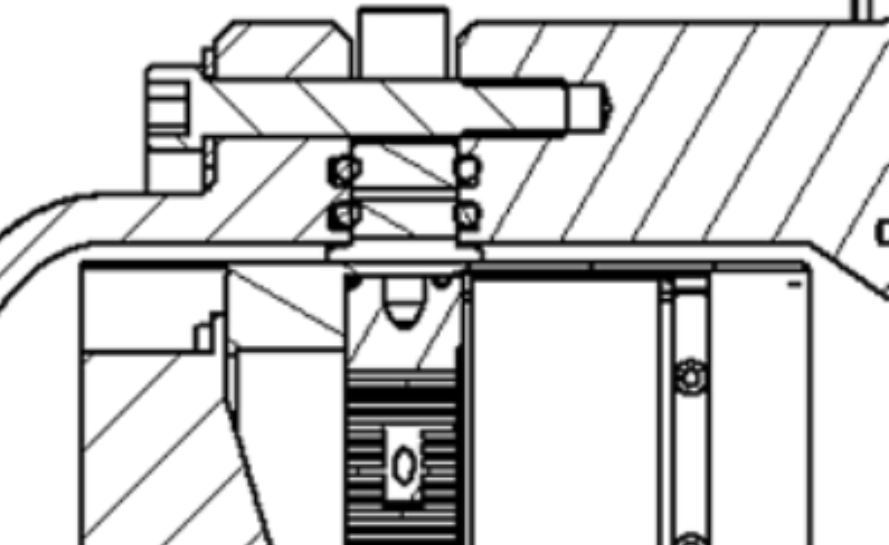
\includegraphics[angle=0,origin=c,width=.35\textwidth]{../fig/fig_TACOTSchematics/TACOT_Cropped.png}};

\draw[black, very thick, dashed, rounded corners] (imagecropped.north west) rectangle (imagecropped.south east);
%\draw[black, very thick, dashed, rounded corners] ($(AHX)+(-1.5cm,3cm)$) rectangle ($(CHX)+(.75cm,-.5cm)$);
	
	\begin{scope}[x={(image.south east)},y={(image.north west)}]
	
%		\filldraw (0,0) circle (2pt); 
%		\filldraw[green] (1,0) circle (1pt);
%		\filldraw[red] (1,1) circle (1pt);		
%		\filldraw[blue] (0,1) circle (1pt);
%		\draw[help lines,xstep=.1,ystep=.1] (0,0) grid (1,1);
%		\fill[orange, rounded corners, opacity=1,draw=orange] (.46,.65) -- ++(132:.09) -- ++(0,-.44) -- ++(48:.09) -- cycle;
		\draw[MatlabYellow,rounded corners,very thick,preaction={fill=MatlabYellow!20,opacity=.5}] (.46,.65) -- ++(132:.09) -- ++(-.03,0) -- ++(0,-.44) --++(.03,0) -- ++(48:.09) -- cycle; %node[left,pos=.5,label={[rotate=90]center:Cavité}]{};
		\draw[MatlabYellow] (.415,0.5) node [label={[rotate=90]center:\textbf{Cône}}]{};
		
%		\draw[blue] (.5,.5) node [anchor=center, preaction={fill=black!20,opacity=.7}] {RIX};
%		\draw[red] (.33,.5) node [anchor=center, preaction={fill=black!20,opacity=.7}] {TA core};	
	
		\draw[MatlabPurple,rounded corners,very thick,preaction={fill=MatlabPurple!20,opacity=.5}] (.365,.7) rectangle (.245,.3) node[pos=.5,label={[rotate=90]center:\textbf{Noyau}}]{};
		
		\node (AHX) at (.27,.65) {};
		\node (Reg) at (.32,.65) {};
		\node (CHX) at (.36,.65) {};
		\node (RIX) at (.77,.4) {};

		\node (HP) at (.19,.4) {};
		
		\draw[<-,very thick,MatlabOrange] (AHX.center) to[out=90,in=0] ($(AHX)+(-.2,.41)$) node[left]{\begin{tabular}{r} Echangeur de chaleur ambiant \\ (HXA) \end{tabular}};		
		\draw[<-,very thick] (Reg.center) to ($(Reg)+(0,.4)$) node[above]{Régénérateur};
		\draw[<-,very thick,MatlabBlue] (CHX.center) to[out=90,in=180] ($(CHX)+(.2,.41)$) node[right]{\begin{tabular}{l} Echangeur de chaleur froid \\ (HXF) \end{tabular}};
		
		\draw[->,very thick,green!50!black] ($(RIX)+(0,-.4)$) -- (RIX.center) node[pos=0,anchor=north]{\begin{tabular}{c}Source acoustique principale \\ (SA1) \end{tabular}};
		\draw[->,very thick,green!50!black] ($(HP)+(0,-.4)$) -- (HP.center) node (SA2) [pos=0,anchor=north]{\begin{tabular}{c}Source acoustique secondaire \\ (SA2) \end{tabular}};
		
%		\draw [white] (.455,.5) node{+};
%		\draw [white] (.41,.65) node{+};
%		\draw [white] (.41,.5) node{+};
%		\draw [white] (.41,.35) node{+};

		\draw[black, very thick, dashed, rounded corners] ($(AHX)+(-.14,.2)$) node(a){} rectangle ($(CHX)+(.07,-.1)$);
		
		\draw[black, very thick, dashed] (a) -- (imagecropped.north east);
		\draw[black, very thick, dashed] ($(a)+(0,-.3)$) -- (imagecropped.south east);
		

	\end{scope}
	
	\draw(imagecropped.south) node[below]{\small \textbf{(a)}};		
	\draw(SA2.south -| image.south) node{\small \textbf{(b)}};
	
\end{tikzpicture}
    \caption{Schéma général du réfrigérateur \textsc{Tacot}.}
    \label{fig:SchemaGeneralTACOT}
\end{figure}

\subsubsection{Noyau thermoacoustique}
Tout comme la machine qui le contient, le noyau adopte une géométrie cylindrique et est composé d'un régénérateur représenté sur la figure~\ref{fig:TacotPhotos_Regen} encadré par deux échangeurs de chaleur. Le premier est l'échangeur ambiant et a pour rôle d'extraire la chaleur qui s'accumule de ce côté du noyau, afin d'éviter l'échauffement global de la machine. Le second est l'échangeur froid, et sa fonction et de simuler une charge thermique à refroidir. Ces échangeurs sont représentés respectivement sur les figures~\ref{fig:TacotPhotos_AHX} et \ref{fig:TacotPhotos_CHX}. Ces trois éléments sont ensuite montés dans une enceinte cylindrique qui se fixe sur le bâti de la machine pour maintenir l'espace nécessaire à la boucle de rétroaction.

\begin{figure}[!ht]
    \centering
	\begin{subfigure}{.3\textwidth}
		\centering
		\external{fig_TacotPhotos_AHX_dansCarter}
		\tikz{\draw(0,0) node{\includegraphics[width=.9\textwidth]{../fig/fig_TacotPhotos/AHX_dansCarter.JPG}};}
		\caption{}
		\label{fig:TacotPhotos_AHX}
	\end{subfigure}		
	\begin{subfigure}{.3\textwidth}
		\centering
		\external{fig_TacotPhotos_Regenerateur}
		\tikz{\draw(0,0) node{\includegraphics[width=.9\textwidth]{../fig/fig_TacotPhotos/Regenerateur.JPG}};}
		\caption{}
		\label{fig:TacotPhotos_Regen}
	\end{subfigure}	
	\begin{subfigure}{.3\textwidth}
		\centering
		\external{fig_TacotPhotos_CHX_dansCarter}
		\tikz{\draw(0,0) node{\includegraphics[width=.9\textwidth]{../fig/fig_TacotPhotos/CHX_dansCarter.JPG}};}
		\caption{}
		\label{fig:TacotPhotos_CHX}
	\end{subfigure}	    
    \caption{Composition du noyau thermoacoustique. \subref{fig:TacotPhotos_AHX} \'Echangeur ambiant, \subref{fig:TacotPhotos_Regen} régénérateur, et \subref{fig:TacotPhotos_CHX} échangeur froid.}
    \label{fig:TacotPhotos}
\end{figure}


Les axes $\mathbf e_x$ et $\mathbf e_r$ sont alors respectivement associés aux directions axiale et radiale du noyau, \echaf{J'arrive pas à relire} avec pour sens positive choisie dans le sens de l'échangeur froid vers l'échangeur ambiant pour le premier, et du centre du noyau vers l'extérieur pour le second.\medskip

\paragraph*{Régénérateur} Le régénérateur est composé de \echaf{combien} disques de tissus métalliques (Gantois, modèle : 102045) empilés dans une enceinte cylindrique de diamètre intérieur $D_{\sf reg}=\qty{148}{\mm}$ et de longueur $L_{\sf reg}=\qty{39}{\mm}$ pour atteindre la porosité $\Phi~=~\qty{68}{\percent}$. Un noyau de cette porosité doit être comparé avec le noyau support des expériences dont les résultats sont publiés par Ramadan \textit{et al.} et dont la porosité vaut \qty{75}{\percent} \cite{ramadan_design_2021}. La quantité de tissus à utiliser pour atteindre la porosité souhaitée s'obtient en utilisant la relation

\begin{align}
	\Phi &= \frac{V_{\sf gaz}}{V_{\sf tot}}, \label{eq:Porosite_Volume}%\\
%	&= \frac{V_{\sf tot}-V_{\sf metal}}{V_{\sf tot}} \nonumber\\
%	&= 1 - \frac{m_{\sf metal}}{m_{\sf tot}} \label{eq:Porosite_Masse}
\end{align}
où $V_{\sf gaz}$ représente le volume occupé par le gaz dans le régénérateur, et $V_{\sf tot}$ le volume total du régénérateur. Le milieu ainsi constitué est poreux et tortueux car l'orientation des disques de tissus est aléatoire, et le rayon hydraulique est défini par  %\echaf{ajouter source pour justifier que les matériaux type "mousse" se comporte comme du cylindrique : UPDATE dans Swift TA unifying... chapitre 7 (tortuous porous media)}

\begin{equation}
	r_h = d_w\frac{\Phi}{4(1-\Phi)},
	\label{eq:DefRayonHydrauGantois}
\end{equation}
avec $d_w$ le diamètre du fil \cite{swift_thermoacoustics_2017}. Ce milieu poreux dispose d'une certaine capacité à laisser passer un écoulement. C'est la perméabilité notée $K_p$, qui est généralement définie par 

\begin{equation}
	K_p = \echaf{v_{\sf ref}\frac{\nu \Delta x}{\Delta P}},
	\label{eq:DefPermeabilite_Wikipedia}
\end{equation}
où $v_{\sf ref}$ est la vitesse d'écoulement d'un fluide de viscosité cinématique $\nu$ causé par un gradient de pression $\frac{\Delta P}{\Delta x}$ de part et d'autre du milieu poreux \cite{nield_convection_2013}. Cependant, il existe dans la littérature des formulations de la perméabilité ne prenant en compte que la géométrie interne du milieu poreux~\cite{dullien_porous_1992}. La formulation retenue s'écrit

\begin{equation}
	K_p = \echaf{\frac{4 r_h^2 \Phi}{8}},
	\label{eq:DefPermeabilite_LISN}
\end{equation}
et donne des résultats satisfaisants pour le developpement des modèles \cite{hireche_experimental_2020}.\bigskip

\echaf{Continuer expl sur travaux de Gaëlle + redériver pour régénérateur}Dans la réalité, les ondes acoustiques en jeu dans les machines thermoacoustiques ne sont ni totalement \og à ondes stationnaires \fg{} (voir le cycle thermodynamique sur la figure~\ref{fig:CycleBrayton}) ni tout à fait \og à ondes progressives \fg{} (dont le cycle est présenté sur la figure~\ref{fig:CycleStirling}). Il a d'ailleurs été montré dans la littérature portant sur les machines à plusieurs sources qu'il existe une vitesse acoustique optimale pour une pression acoustique donnée~\cite{poignand_etude_2006}. Les puissances thermiques pompées et le gradient de températures le long du régénérateur sont les plus élevées lorsque la vitesse acoustique atteint une amplitude donnée par

\begin{subequations}
	\begin{align}
		|u|_{\sf opt} &= \sqrt{\frac{4\omega\left(\echaf{kh+k_se_s}\right)\left(1-\Prandtl^2\right)\left(\echaf{1-\frac{\delta_\nu}{h}+\frac{\delta_\nu^2}{2h^2}}\right)}{\delta_\kappa \rho_0 C_p \left(1-\Prandtl\sqrt{\Prandtl}\right)}},	\label{eq:u_mag_opt_Gaelle}\\
		\intertext{et un déphasage écrit}
		\angle u_{\sf opt} &= \arctan\left[-\frac{1+\sqrt{\Prandtl}-\frac{\delta_\nu}{h}}{1-\sqrt{\Prandtl}+\frac{\delta_\nu}{h}\sqrt{\Prandtl}}\right].	\label{eq:u_arg_opt_Gaelle}
	\end{align}
	\label{eq:u_opt_Gaelle}
\end{subequations}
\echaf{Remplacer $kh+k_s e_s$ par $\Phi k + (1-\Phi)k_s$ ?}

Cette machine nécessite entre autres choses le respect de la condition $\delta_{\kappa,\nu} \gg r_h$, de sorte à avoir un excellent contact thermique entre le fluide et le solide poreux. Pour le fluide considéré, les épaisseurs de couches limites sont tracées en fonction de la fréquence et comparé au rayon hydraulique sur la figure~\ref{fig:dKdV}.

\begin{figure}[!ht]
    \centering
    \external{fig_dKdV}
%    \externalremake
    \begin{tikzpicture}
    \def\width{.9*\textwidth};
    \def\height{.45*\width};
    \def\spx{.25cm};
    \def\spy{1.25cm};
    \def\legx{.5cm};
    \def\legy{\legx};
    \def\prop{.45};
    \def\xcursor{47};
    \def\ycursorV{9.112e-5};
    \def\ycursorK{1.4452e-4};
    \def\rh{2.81e-5};
    
    \begin{axis}[name=dKdV,width={\width},height={\height},
    grid=both, minor tick num=10, 
    grid style={line width=.1pt, draw=gray!10},
    major grid style={line width=.2pt,draw=gray!50},
    xlabel={Fréquence $f$ [\unit{\Hz}]},
    ylabel={\'Epaisseurs de couches limites $\delta_{\kappa,\nu}$ [\unit{\m}]},
    xmin=0,xmax=75,ymin=0,ymax=.5/1000,
    xtick={0,25,50,75,100},
    extra x ticks={47},
    extra x tick style={
        grid=major,
        xticklabel={\num{47}},
        xticklabel style={yshift=0, anchor=north}
        },
    extra y ticks={\rh},
    extra y tick style={
        grid=major,
        yticklabel={$r_h$},
        yticklabel style={yshift=1mm, anchor=east}
        },
    ytick={0,1e-4,...,10e-4},
%    ytick={0,2.81/100000,9.1120/100000,1.4452/10000,
%    	2.5/10000,5/10000,1/1000},
    scaled y ticks = false,
    domain=0:100,
    legend cell align={left},
    legend style = {at={($(1,1)+(-2mm,-2mm)$)},anchor = north east,rounded corners}
    ]
        \addplot[solid,ultra thick,draw=Plasma1] file {../fig/fig_dKdV/data/data_dK.txt};
        \addplot[solid,ultra thick,draw=Plasma64] file {../fig/fig_dKdV/data/data_dV.txt};
        \filldraw[Plasma1] (\xcursor,\ycursorK) circle (2pt) node[above right]{$\delta_\kappa=\qty{\ycursorK}{\meter}$};
        \filldraw[Plasma64] (\xcursor,\ycursorV) circle (2pt) node[below left]{$\delta_\nu=\qty{\ycursorV}{\meter}$};
%        \draw[dashed,black!50] (\xcursor,0) -- (\xcursor,\ycursorK);
%        \draw[dashed,Plasma33] (\xcursor,\ycursorK) -- (0,\ycursorK) node[left]{\num{1.4452e-4}};
%        \draw[dashed,Plasma66] (\xcursor,\ycursorV) -- (0,\ycursorV) node[left]{\num{9.1120e-5}};
%         \draw[dashed,black!50] ({axis cs:\xcursor,0}|-{rel axis cs:0,0}) -- ({axis cs:\xcursor,0}|-{rel axis cs:0,\ycursorK});
       \addplot[loosely dashed,draw=black, ultra thick] {\rh};
       \draw(0,\rh) node[above right]{\qty{\rh}{\meter}};
        
        \legend{$\delta_\kappa$ \\ $\delta_\nu$ \\ $r_h$ \\};
    \end{axis}
\end{tikzpicture}
    \caption{\'Evolution des épaisseurs de couches limites thermique $\delta_\kappa$ et visqueuse $\delta_\nu$ en fonction de la fréquence, définies par le système d'équations~\eqref{eq:CouchesLimites}. Elles sont comparées au rayon hydraulique $r_h$.}
    \label{fig:dKdV}
\end{figure}

Les dimensions et paramètres du régénérateur sont résumés dans le tableau \ref{tab:ParamHydrauTAC}.

\begin{table}[!ht]
    \caption{Paramètres hydrauliques du régénérateur à la fréquence de fonctionnement, \linebreak $f=\qty{47}{\Hz}$}
    \label{tab:ParamHydrauTAC}
    \centering
    \begin{tabular}{l@{\hspace{1cm}}l}
    	\hline
    	\textbf{Paramètre [unité]} & \textbf{Valeur} \\\hline\hline
    	Diamètre du noyau $D_{\sf reg}$ [\unit{\meter}] & \num{148e-3} \\
    	Longueur du régénérateur $L_{\sf reg}$ [\unit{\meter}] & \num{39e-3} \\
    	Diamètre du fil $d_w$ [\unit{\meter}] & \num{53e-6} \\
        Rayon hydraulique $r_h$ [\unit{\meter}] & \num{2.81e-5} \\
        Porosité du noyau $\Phi$ [\unit{\percent}] & \num{68}\\
        Couche limite thermique $\delta_\kappa$ [\unit{\meter}] & \num{1.4452e-4} \\
        Couche limite visqueuse $\delta_\nu$ [\unit{\meter}] & \num{9.1120e-5} \\
        \echaf{Perméabilité} [\unit{\meter\squared}] & \num{2.68e-10} \\
        \hline
    \end{tabular}
\end{table}

\paragraph*{\'Echangeurs de chaleur}
Le pompage de chaleur par effet thermoacoustique doit être exploité. En effet, dans l'application du \textsc{Tacot}, \echaf{blablabla}

\subsection{Instrumentation}
L'instrumentation utilisée est basée sur celle conçue au début du projet \cite{ramadan_design_2021}, tout en modifiant quelques éléments.\bigskip


\subsubsection{Chaîne d'excitation}
Premièrement, la chaîne d'excitation est présentée. Elle est assez simple, et se compose d'un générateur de fonction à deux canaux (TekTronix AFG3022). Chaque canal est ensuite connecté à un amplificateur pour chaque source acoustique. La source principale (RIX Industries, 1S241M) est alimentée par un amplificateur QSC PLD4.5, et la source secondaire (Peerless, GBS135F) par un amplificateur Yamaha P3500S.\medskip


\subsubsection{Chaîne d'acquisition}
La chaîne d'acquisition se compose de plus de trente capteurs. Tous ne sont pas utilisés, mais peuvent servir de contrôle durant une expérience, pour s'assurer du bon déroulement de celle-ci.

\paragraph*{Alimentation électrique des sources} L'alimentation électrique de la source acoustique principale est mesurée au moyen d'une sonde différentielle pour la tension \echaf{et le courant ?}. Pour la source acoustique secondaire, un multimètre et une pince de courant se chargent de mesurer sa consommation électrique. En parallèle, les tensions aux bornes des deux sources sont affichées sur un oscilloscope pour s'assurer de leur déphasage.

\paragraph*{Température} Dix-neuf thermocouples Type K de \qty{.5}{\milli\meter} de diamètre sont placés de la manière suivante : quinze thermocouples mesurent la température en différentes positions du noyau, un devant la source acoustique principale, deux derrière celle-ci, et un derrière la source acoustique secondaire. Cependant, la carte d'acquisition utilisée (National Instruments, NI9213) ne comporte que seize entrées, il \echaf{convient} donc suivant les informations recherchée dans une expérimentation de sélectionner les trois thermocouples dont les signaux ne sont pas enregistrés. Dans tous les résultats de mesures discutés dans la suite, les thermocouples du noyau et de devant la source acoustique principale sont connectés. Le placement de ces thermocouples d'intérêt est représenté sur la figure~\ref{fig:TCdansNoyau} par les symboles `\textcolor{cyan}{\textbullet}'.

\begin{figure}[!ht]
    \centering
    \external{fig_TCdansNoyau}
    %\externalremake
    \begin{tikzpicture}[scale=.2]
	\def\rCHX{14cm};
	\def\lCHX{.7cm};
	\def\rREG{14.8cm};
	\def\lREG{3.9cm};
	\def\rAHX{11cm};
	\def\lAHX{2.3cm};
	
	
	\fill[pattern=horizontal lines,pattern color=MatlabOrange,draw=black] (0,-\rAHX) rectangle ++(\lAHX,2*\rAHX);
	\draw[MatlabOrange] (0,-\rAHX) node(AHX)[below left]{\'Echangeur ambiant};
	\foreach \r in {-.9,0,.9}{
		\draw[cyan] (-.15*\lREG,\r*\rAHX) node{\textbullet};
	}
	\filldraw[draw=black,fill=gray!50!white] (0,\rAHX) rectangle (\lAHX,\rREG);		% côtés où l'eau circule
	\filldraw[draw=black,fill=gray!50!white] (0,-\rAHX) rectangle (\lAHX,-\rREG);	%
	
	\draw[MatlabOrange,->] (AHX.north) to[out=90,in=180] (-.1*\lCHX,-.5*\rAHX);
	
	\begin{scope}[xshift=\lAHX] % Reg
		\fill[pattern=crosshatch,pattern color=gray,draw=black] (0,-\rREG) rectangle ++(\lREG,2*\rREG);
		\draw[black] (\lREG/2,\rREG) node[above]{Régénérateur};		
		\foreach \x in {.15,.5,.85}{
			\foreach \r in {-.9,0,.9}{
				\draw[cyan] (\x*\lREG,\r*\rREG) node{\textbullet};
		}}
	\end{scope}
	
	\begin{scope}[xshift=\lAHX+\lREG] % CHX
		\fill[pattern=horizontal lines,pattern color=MatlabBlue,draw=black] (0,-\rCHX) rectangle ++(\lCHX,2*\rCHX);
		\draw[MatlabBlue] (\lCHX,-\rCHX) node(CHX)[below right]{\'Echangeur froid};
		\foreach \r in {-.9,0,.9}{
		\draw[cyan] (\lCHX+.15*\lREG,\r*\rCHX) node{\textbullet};
	}
	\filldraw[draw=black,fill=gray!50!white] (0,\rREG) rectangle (\lCHX,\rCHX);		% côtés où l'eau circule
	\filldraw[draw=black,fill=gray!50!white] (0,-\rREG) rectangle (\lCHX,-\rCHX);	%
	
	\draw[MatlabBlue,->] (CHX.north) to[out=90,in=0] (1.1*\lCHX,-.5*\rCHX);
	\end{scope}
	
	\draw[green!50!black] (0,0) node[left]{\begin{tabular}{rl}Source & \\ acoustique & $\leftarrow$ \\ secondaire &\end{tabular}};
	\draw[green!50!black] ({\lCHX+\lREG+\lAHX},0) node[right]{\begin{tabular}{rl}	
	 & Source \\ $\rightarrow$ \textcolor{cyan}{\textbullet} & acoustique \\ & principale\end{tabular}};
	
\end{tikzpicture}
    \caption{Emplacement des thermocouples dans le noyau thermoacoustique. Zoom sur l'encadré violet de la figure~\ref{fig:SchemaGeneralTACOT}.}
    \label{fig:TCdansNoyau}
\end{figure}

\paragraph*{Pression dynamique} Quatre sondes piézoélectriques (PCB Piezotronics, 113B28) captent les oscillations de pression dans la pompe à chaleur. Deux sont placées à l'arrière de chacune des sources acoustiques, et les deux autres dans le canal de rétroaction de la cavité thermoacoustique. Les capteurs sont ensuite connectés à une carte d'acquisition (National Instruments, NI9234). 
%Toutefois, la longueur d'onde dans le mélange de gaz vaut $\lambda=\qty{11.7}{\meter}$ à la fréquence de fonctionnement $f=\qty{47}{\hertz}$ et est suffisamment grande pour garantir une amplitude de pression constante dans toute la machine.

\paragraph*{Pression statique} Deux capteurs (Endress, Cerabar PMP21) sont connectés sur les deux tuyaux d'alimentation en gaz de la pompe  à chaleur d'un côté, et sur une carte d'acquisition (National Instruments, NI9234) de l'autre. Les arrivées de gaz se trouvent de part et d'autre de la source acoustique principale et ont pour but d'éviter une surpression sur sa face avant ou arrière et son endommagement.

\paragraph*{Puissance extraite par l'échangeur ambiant} Le fonctionnement de cet échangeur est détaillé dans l'annexe~\ref{chap:AHX}. Pour déterminer la quantité de chaleur extraite du côté ambiant du noyau, la différence de température entre l'entrée d'eau de l'échangeur et sa sortie d'eau est mesurée grâce à deux sondes de platine PT100 connectées sur une carte d'acquisition (National Instruments, NI9217).

\paragraph*{Déplacement des sources} Le piston de chaque source acoustique est équipé d'un accéléromètre. Pour la source acoustique principale, l'accéléromètre (MMF, KS91C) est collé sur la face arrière, tandis que pour la source secondaire, le capteur (PCB Piezotronics, 352C23) est collé sur la face avant. Ces capteurs sont choisis de sorte à ne pas trop varier la masse de l'équipage mobile, en particulier pour la source secondaire où la masse du piston et celle de l'ensemble accéléromètre et câble sont du même ordre de grandeur.\bigskip

Toutes les connexions entre l'intérieur de la machine sous haute pression statique et l'extérieur se font via des traversées étanches. Pour les capteurs, il s'agit de HF2-8CU+16K de Spectite, dimensionnées pour \qty{550}{\bar}. Pour les sources acoustiques, une traversée FA17613 de Solid Sealing Technology est choisie, et pour la source acoustique secondaire, le modèle FA36735 du même fabricant est retenu.

%Les signaux de tensions aux bornes des sources acoustiques sont acquis par une carte d'acquisition (National Instruments, (\echaf{modèle}), après connexion à une sonde de tension (\echaf{modèle}). Deux accéléromètres (\echaf{modèle}) sont collés sur les sources pour mesurer leur déplacement. Pour connaître la pression acoustique dans la cavité thermoacoustique, quatre sondes (\echaf{modèle}) sont placées respectivement à l'arrière de la source principale, à l'arrière de la source secondaire 


%\begin{figure}[!ht]
%    \centering
%    \external{fig_ChaineAcqui}
%    %\externalremake
%    \begin{tikzpicture}
	\draw (0,0) --++(1,0);
\end{tikzpicture}
%    \caption{Carte de la chaine d'acquisition et d'alimentation du réfrigérateur TACOT}
%    \label{fig:ChaineAcqui}
%\end{figure}

%\begin{itemize}
%    \item GBF
%    \item Amplis
%    \begin{itemize}
%        \item QSC
%        \item Yamaha
%    \end{itemize}
%    \item Sondes de tension
%    \item Cartes NI
%    \begin{itemize}
%        \item Pression statique
%        \item Pression dynamique
%        \item Thermocouples
%        \item PT100
%        \item Accéléromètres
%    \end{itemize}
%    \item LabVIEW d'acquisition
%\end{itemize}

%Pour étudier la distribution de température le long de l'axe du noyau, ainsi que dans les dimensions transverses, Seize thermocouples sont placés sur un plan et représentés par les symboles~`\textcolor{cyan}{\textbullet}' sur la figure~\ref{fig:TCdansNoyau}. Neuf sont placés au c\oe{}ur du noyau, dans le régénérateur. Trois sont fixés à l'extérieur du noyau, hors de l'échangeur ambiant, et trois autres sur l'extérieur de l'échangeur froid. Enfin, un dernier thermocouple est positionné au voisinage de la source acoustique principale, en vis-à-vis de l'échangeur froid.



%\subsection{Emplacement des capteurs}
%
%\begin{figure}[!ht]
%    \centering
%    \external{fig_ThermocouplesDefinition}
%    %\externalremake
%    \begin{tikzpicture}
    \def\LX{1};
    \def\LY{2};
    \def\CoreX{1.5};
    \def\CoreY{.9*\LY};
    
    \draw[line width=.5mm] (-2.5*\LX,0) to[out=90,in=-180] (-\LX,\LY) -- ++(2*\LX,0) -- ++(.5*\LX,-2*\LY/3) -- ++(.2*\LX,0) -- ++(0,2*\LY/3);
\draw[line width=.5mm] (\LX,\LY) -- ++(\LX,0) to[out=0,in=90] (3.5*\LX,0);

\draw[line width=.5mm] (-\LX,\CoreY) -- ++(\CoreX,0);
\draw[fill=PythonBlue] (-.9*\LX,0) -- ++(0,\CoreY) to[out=-80,in=90] (-.7*\LX,0);
\draw ({-\LX+.4*\CoreX},0) -- ++(0,\CoreY);
\draw ({-\LX+.9*\CoreX},0) -- ++(0,\CoreY);

\draw[fill=PythonBlue] (1.6*\LX,0) |- ++(.3*\LX,.9*\LY/3) |- ++(\LX,.2*\LY) arc (90:0:.05) -- ++(0,-.5*\LY);
    
    \begin{scope}[xscale=1,yscale=-1]
        \draw[line width=.5mm] (-2.5*\LX,0) to[out=90,in=-180] (-\LX,\LY) -- ++(2*\LX,0) -- ++(.5*\LX,-2*\LY/3) -- ++(.2*\LX,0) -- ++(0,2*\LY/3);
\draw[line width=.5mm] (\LX,\LY) -- ++(\LX,0) to[out=0,in=90] (3.5*\LX,0);

\draw[line width=.5mm] (-\LX,\CoreY) -- ++(\CoreX,0);
\draw[fill=PythonBlue] (-.9*\LX,0) -- ++(0,\CoreY) to[out=-80,in=90] (-.7*\LX,0);
\draw ({-\LX+.4*\CoreX},0) -- ++(0,\CoreY);
\draw ({-\LX+.9*\CoreX},0) -- ++(0,\CoreY);

\draw[fill=PythonBlue] (1.6*\LX,0) |- ++(.3*\LX,.9*\LY/3) |- ++(\LX,.2*\LY) arc (90:0:.05) -- ++(0,-.5*\LY);
    \end{scope}
    
    
    \draw[dashed,rounded corners,PythonRed] (.55,.95*\LY) rectangle ++(-.75*\CoreX,-1.9*\LY) node[midway]{\rotatebox{90}{Noyau TA}};
    
    \begin{scope}[xshift=5cm,xscale=2.5,yscale=2]
        \draw (0,0) |- ++(2,1.5) -- ++(0,-1.5);
        \draw (.5,0) -- ++(0,1.5);
        \draw (1.5,0) -- ++(0,1.5);
        \draw[line width=1mm] (-.2,1.5) -- ++(2.4,0);
    
        \begin{scope}[xscale=1,yscale=-1]
            \draw (0,0) |- ++(2,1.5) -- ++(0,-1.5);
            \draw (.5,0) -- ++(0,1.5);
            \draw (1.5,0) -- ++(0,1.5);
            \draw[line width=1mm] (-.2,1.5) -- ++(2.4,0);
        \end{scope}
        % \foreach \x [evaluate=\x] in {0,...,4}{
        %     \foreach \y [evaluate=\y] in {1,...,3}{
        %     \draw (\x,\y) node[]{$t$};}}
    \end{scope}
    
    %\draw[line width=1mm] (5*\LX,.5*\LY) -- ++(6*\LX,0);
    %\draw[line width=1mm] (5*\LX,-.5*\LY) -- ++(6*\LX,0);
    %
    %\draw (-2.5*\LX,\LY) node[above]{\bf (a)};
    %\draw (5*\LX,\LY) node[above]{\bf (b)};
    
\end{tikzpicture}
%    \caption{Emplacements des thermocouples dans le noyau thermoacoustique}
%    \label{fig:ThermocouplesDefinition}
%\end{figure}

\section{Protocole expérimental}\label{chap:ProtocolExpe}
Pour l'étude de l'influence de la gravité sur la distribution de température dans son noyau et ses performances, le réfrigérateur doit pouvoir être orienté dans toutes les orientations utiles. Pour ce faire, il est suspendu par des palans grâce aux fixations situées à ses extrémité  et au milieu dans le sens de sa longueur. La figure~\ref{fig:TACOTSuspendu_Frigo} présente le réfrigérateur accroché à ses extrémités, et la figure~\ref{fig:TACOTSuspendu_Palans} les trois palans pour le soutenir. Les deux palans de couleur grise, initialement présents pour régler l'inclinaison de la pompe à chaleur par rapport à l'axe horizontal, et le troisième de couleur bleue pour ajouter une direction de rotation autour de l'axe de symétrie. Celui-ci permet en outre de plus aisément passer d'une orientation à l'autre. 

\begin{figure}[!ht]
    \centering
	\begin{subfigure}{.45\textwidth}
		\centering
		\external{fig_SystemeAccroche_Machine}
		\tikz{\draw(0,0) node{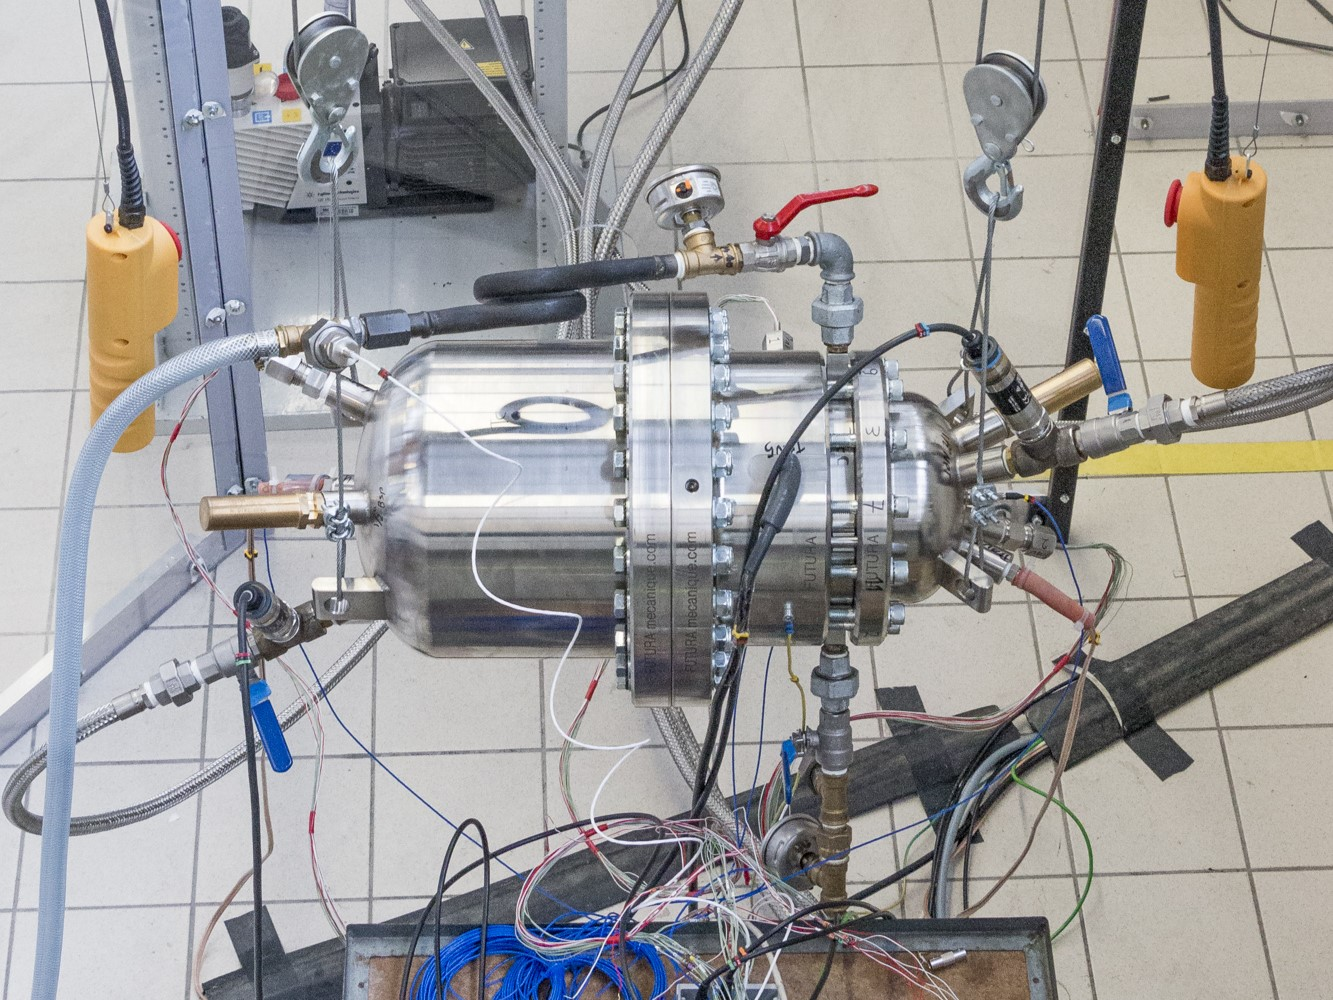
\includegraphics[width=.9\textwidth]{../fig/fig_SystemeAccroche/Machine_horizBetter_cropped.jpg}};}
		\caption{}
		\label{fig:TACOTSuspendu_Frigo}
	\end{subfigure}		%
	\begin{subfigure}{.45\textwidth}
		\centering
		\external{fig_SystemeAccroche_Palan}
		\tikz{\draw(0,0) node{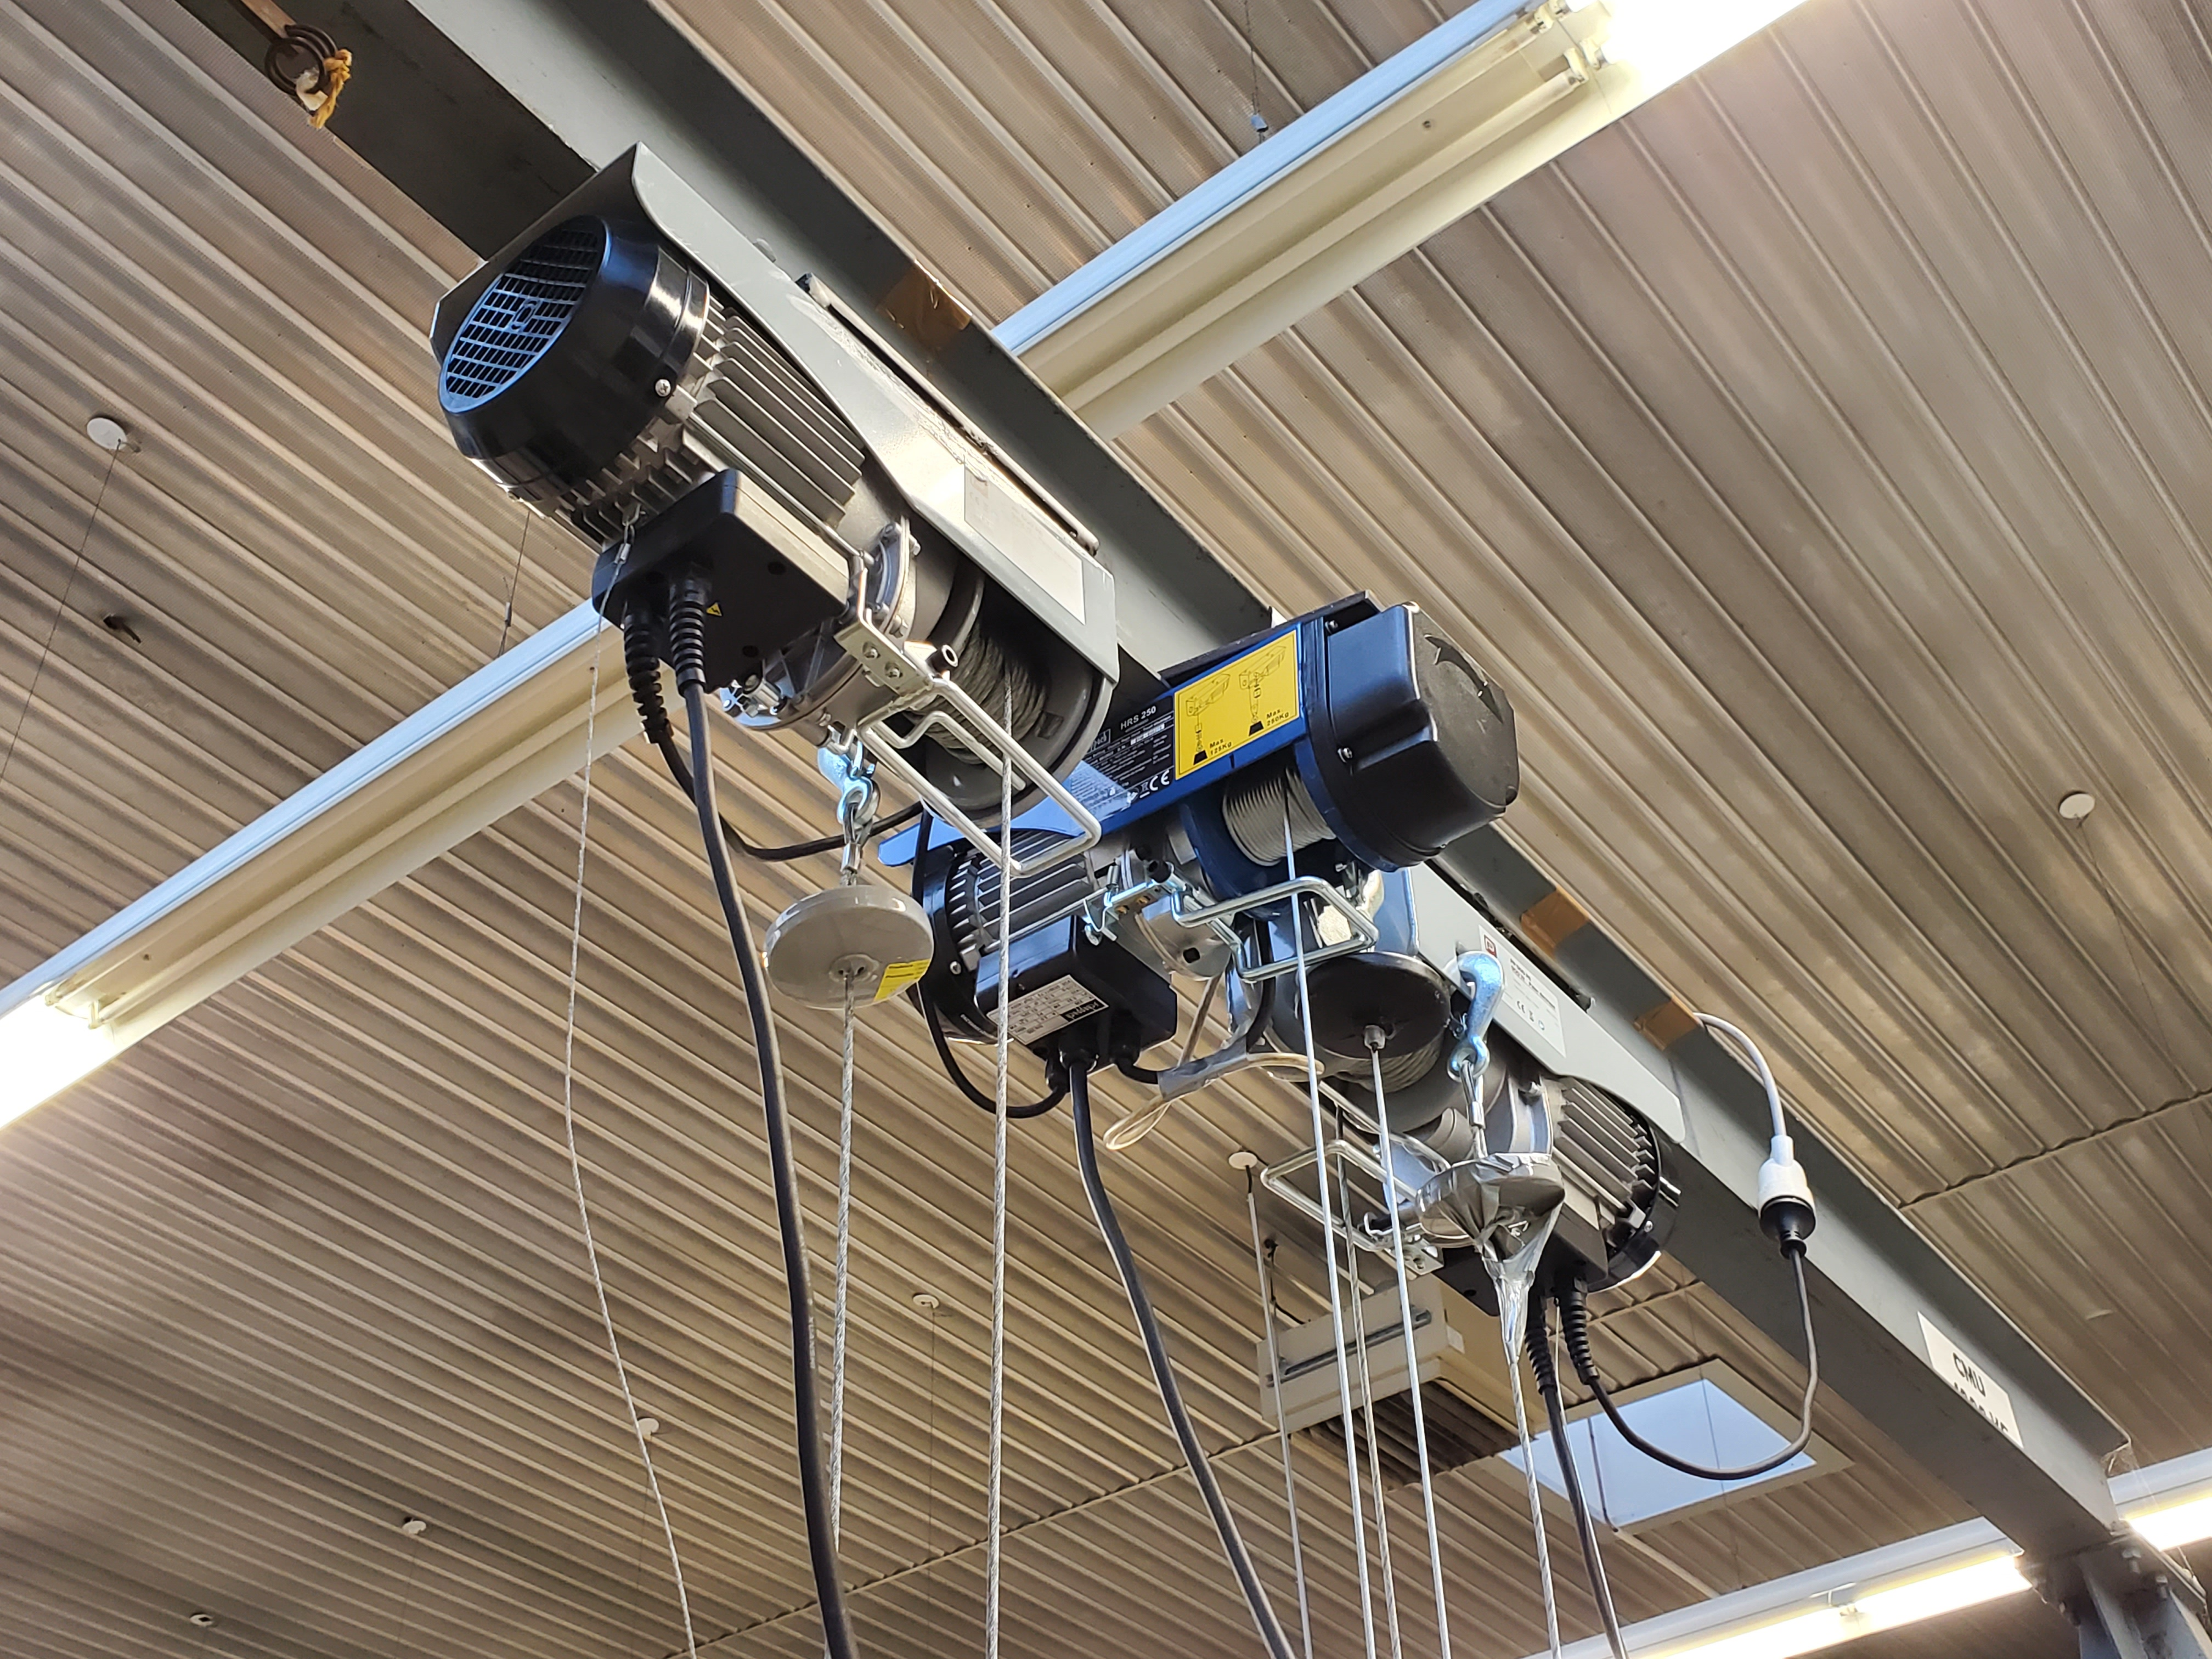
\includegraphics[width=.9\textwidth]{../fig/fig_SystemeAccroche/Palans.jpg}};}
		\caption{}
		\label{fig:TACOTSuspendu_Palans}
	\end{subfigure}	    
    \caption{Photographies \subref{fig:TACOTSuspendu_Frigo} du refrigérateur accroché et \subref{fig:TACOTSuspendu_Palans} des palans formant le système de suspension.}
    \label{fig:TACOTSuspendu}
\end{figure}

\subsection{Définition des orientations}

Les orientations choisies au moyen des palans sont décrites par deux angles $\psi_v$ et $\psi_h$. Le premier désigne l'angle entre l'axe horizontal et l'axe de symétrie du réfrigérateur, tandis que le second, la rotation autour de cet axe de symétrie. Les orientations utilisées dans les différentes parties de ce manuscript sont présentées sur la figure~\ref{fig:OrientationCore}. Cette figure, dans laquelle la gravité est toujours dirigée vers le bas de la page, présente également les emplacements et les numéros d'identification des thermocouples utilisés.\medskip

\begin{figure}[!ht]
    \centering
	\begin{subfigure}[c]{.4\textwidth}
		\centering
		\external{fig_OrientationCore_H1}
%    	\externalremake
		\begin{tikzpicture}[scale=2/3]

%    \def\lenreg{2};
%    \def\diam{3};
    \def\spy{2};
    \def\xdist{8cm};
    \def\ydist{-7cm};
%    \def\persp{20};
%    
%    \def\LX{1};
%    \def\LY{2};
%    \def\CoreX{1.5};
%    \def\CoreY{.9*\LY};
%    

	\def\L{2.1};
	\def\R{5};
	\def\HX{.25};
	\def\decalage{\R/2-\L/2};
	
		\draw(6.5,\R/2) node{\includegraphics[width=.8\textwidth]{../fig/fig_OrientationCore/tex/TACOT.png}};
			
		\fill[right color=blue!25,left color=red!25, draw=black] (\decalage,0) rectangle ++(\L,\R);
		\draw[fill=red!25] (\decalage,0) rectangle ++(-\HX,\R);
		\draw[fill=blue!25] (\decalage+\L,0) rectangle ++(\HX,\R);

		\foreach \z [evaluate=\z] in {0,...,4}{
			\foreach \r [evaluate=\r as \num using int(\r+1 + 3*\z)] in {0,...,2}{
				\draw ({\decalage+.5+\L-\z*(1+\L)/4},{-(\R-.4)/2*\r+\R-.2}) node[minimum size=10pt,draw,circle,fill=white,opacity=.7,text opacity=1]{} node(n\z\r){\scriptsize \num};
}}

%		\draw (n01.east) node [right]{0 $\rightarrow$ \begin{tabular}{l}Source\\acoustique\\principale\end{tabular}};
		\draw ($(n01)+(1.5,0)$) node[minimum size=10pt,draw,circle,fill=white,opacity=.7,text opacity=1]{} node(RIX) {\scriptsize 0};% node[anchor=west]{\begin{tabular}{rl}
%		& Source\\
%		$\rightarrow$ & acoustique\\
%		& principale
%		\end{tabular}};
		\draw (n30.north west) node [above, fill=white, fill opacity=.7, text opacity=1]{Ambiant};
		\draw (n10.north east) node [above, fill=white, fill opacity=.7, text opacity=1]{Froid};
\end{tikzpicture}
		\caption{`\texttt{H1}'}
		\label{fig:OrientationCore_H1}
	\end{subfigure}
	
	\begin{subfigure}[c]{.4\textwidth}
		\centering
		\external{fig_OrientationCore_H2}
%    	\externalremake
		\begin{tikzpicture}[scale=2/3]

%    \def\lenreg{2};
%    \def\diam{3};
    \def\spy{2};
    \def\xdist{8cm};
    \def\ydist{-7cm};
%    \def\persp{20};
%    
%    \def\LX{1};
%    \def\LY{2};
%    \def\CoreX{1.5};
%    \def\CoreY{.9*\LY};
%    

	\def\L{1};
	\def\R{5};
	\def\HX{.25};
	\def\decalage{\R/2-\L/2};
	
%	\draw[opacity=0] (\decalage,0) rectangle ++(-\HX,\R); %%% Pour l'alignement vertical
%\draw{[white](\L/2,0) -- ++(0,\R);
	
	\begin{scope}[yslant=-1]
		\begin{scope}[xslant=.71]%, rotate=90, xscale=1]
		\node at (\decalage-\HX,0) (NewO) {};
%		\draw[->, very thick] (NewO.center) -- ++(0,1.2*\R);
%		\draw[->, very thick] (NewO.center) -- ++(1.2*\R,0);
		
		\fill[shading=axis,right color=MatlabBlue,left color=MatlabOrange, shading angle=22.5, draw=black] (\decalage,0) rectangle ++(\L,\R*1.4);
		\draw[fill=MatlabOrange] (\decalage,0) rectangle ++(-\HX,\R*1.4);
		\draw[fill=MatlabBlue] (\decalage+\L,0) rectangle ++(\HX,\R*1.4);

		\foreach \z [evaluate=\z] in {0,...,4}{
			\foreach \r [evaluate=\r as \num using int(\r+1 + 3*\z)] in {0,...,2}{
				\draw ({\decalage+.5+\L-\z*(1+\L)/4},{-(\R*1.4-.4)/2*\r+\R*1.4-.2}) node[minimum size=10pt,draw,circle,fill=white,opacity=.7,text opacity=1]{} node(n\z\r){\scriptsize \num};
}}

%		\draw (n01.east) node [right]{$\rightarrow$ \begin{tabular}{l}Source\\acoustique\\principale\end{tabular}};
		\draw ($(n01)+(.75,0)$) node[minimum size=10pt,draw,circle,fill=white,opacity=.7,text opacity=1]{} node {\scriptsize 0};% node[anchor=west]{\begin{tabular}{rl}
%		& Src\\
%		$\rightarrow$ & ac\\
%		& princ
%		\end{tabular}};
%		\draw (n30.north west) node [above right, fill=white, fill opacity=0, text opacity=1]{\textcolor{MatlabOrange}{\textbf{Ambiant}}};
%		\draw (n10.north east) node [above right, fill=white, fill opacity=0, text opacity=1]{\textcolor{MatlabBlue}{\textbf{Froid}}};
		
	\end{scope}
	\end{scope}
	\begin{pgfonlayer}{background}
		\draw[->, very thick] (NewO.center) -- ++(22.5:1.2*\R) node [above] {$\mathbf e_{y,0}$};
		\draw[->, very thick] (NewO.center) -- ++(90:1.2*\R) node [left] {$\mathbf e_{z,0}$};
		\draw[->, very thick] (NewO.center) -- ++(-45:1.2*\R) node [right] {$\mathbf e_{x,0}$};
  	\end{pgfonlayer}
\end{tikzpicture}
		\caption{`\texttt{H2}'}
		\label{fig:OrientationCore_H2}
	\end{subfigure} \vspace{1cm}
	
	\begin{subfigure}[c]{.4\textwidth}
		\centering
		\external{fig_OrientationCore_V1}
%    	\externalremake
		%\fill[top color=red!25, bottom color=blue!25, draw=black] (0,0) rectangle ++(\R,\L);
%\draw[fill=blue!25] (0,0) rectangle ++(\R,-\HX);
%\draw[fill=red!25] (0,\L) rectangle ++(\R,\HX);
%
%\foreach \z [evaluate=\z] in {0,...,4}{
%	\foreach \r [evaluate=\r as \num using int(\r+1 + 3*\z)] in {0,...,2}{
%		\draw ({-(\R-.4)/2*\r+\R-.2},{\z*(1+\L)/4-.5}) node(n\z\r){\num};
%}}
%
%\draw (n40.south east) node [right]{AHX};
%\draw (n00.north east) node[right]{CHX};
%\draw (n01.south) node [below]{\shortstack{ $\downarrow$ \\Source acoustique principale}};
%
%\draw (0,\L+2*\HX+\spy) node [anchor=west]{\textbf{(c)} \texttt{V1}};

\begin{tikzpicture}[scale=2/3]

%    \def\lenreg{2};
%    \def\diam{3};
    \def\spy{2};
    \def\xdist{8cm};
    \def\ydist{-7cm};
%    \def\persp{20};
%    
%    \def\LX{1};
%    \def\LY{2};
%    \def\CoreX{1.5};
%    \def\CoreY{.9*\LY};
%    

	\def\L{2};
	\def\R{5};
	\def\HX{.35};
	\def\decalage{\R/2-\L/2};
	
	\begin{scope}[yslant=tan(22.5)]	
		
		\node at (0,-\HX) (NewO) {};
	
		\fill[shading=axis,right color=MatlabBlue,left color=MatlabOrange, shading angle=22.5, draw=black] (0,0) rectangle ++(\R,\L);
		\draw[fill=MatlabBlue] (0,0) rectangle ++(\R,-\HX);
		\draw[fill=MatlabOrange] (0,\L) rectangle ++(\R,\HX);

		\foreach \z [evaluate=\z] in {0,...,4}{
			\foreach \r [evaluate=\r as \num using int(\r+1 + 3*\z)] in {0,...,2}{
				\draw ({-(\R-.4)/2*\r+\R-.2},{\z*(1+\L)/4-.5}) node[minimum size=10pt,draw,circle,fill=white,opacity=.7,text opacity=1]{} node(n\z\r){\scriptsize \num};
}}

%		\draw (n40.south east) node [right, fill=white, fill opacity=0, text opacity=1]{\textcolor{MatlabOrange}{\textbf{Ambiant}}};
%		\draw (n00.north east) node[right, fill=white, fill opacity=0, text opacity=1]{\textcolor{MatlabBlue}{\textbf{Froid}}};
		\draw ($(n01.south)+(0,-1.1)$) node[minimum size=10pt,draw,circle,fill=white,opacity=.7,text opacity=1]{} node (RIX){\scriptsize 0};% node[anchor=north]{\begin{tabular}{c}
%		$\downarrow$\\
%		Source acoustique principale
%		\end{tabular}};

	\end{scope}
	\begin{pgfonlayer}{background}
		\draw[->, very thick] (NewO.center) -- ++(22.5:1.2*\R) node [above] {$\mathbf e_{y,0}$};
		\draw[->, very thick] (NewO.center) -- ++(90:1.2*\R) node [left] {$\mathbf e_{z,0}$};
		\draw[->, very thick] (NewO.center) -- ++(-45:1.2*\R) node [right] {$\mathbf e_{x,0}$};
  	\end{pgfonlayer}		
\end{tikzpicture}
		\caption{`\texttt{V1}'}
		\label{fig:OrientationCore_V1}
	\end{subfigure} 
	
	\begin{subfigure}[c]{.4\textwidth}
		\centering
		\external{fig_OrientationCore_V2}
%    	\externalremake
		%\fill[top color=blue!25, bottom color=red!25, draw=black] (0,0) rectangle ++(\R,\L);
%\draw[fill=red!25] (0,0) rectangle ++(\R,-\HX);
%\draw[fill=blue!25] (0,\L) rectangle ++(\R,\HX);
%
%\foreach \z [evaluate=\z] in {0,...,4}{
%	\foreach \r [evaluate=\r as \num using int(\r+1 + 3*\z)] in {0,...,2}{
%		\draw ({(\R-.4)/2*\r+.2},{-\z*(1+\L)/4+\L+.5}) node(n\z\r){\num};
%}}
%
%\draw (n01.north) node [above]{\shortstack{Source acoustique principale\\ $\uparrow$}};
%\draw (n42.north east) node [right]{AHX};
%\draw (n02.south east) node [right]{CHX};
%
%\draw (0,\L+2*\HX+\spy) node [anchor=west]{\textbf{(d)} \texttt{V2}};

\begin{tikzpicture}[scale=2/3]

%    \def\lenreg{2};
%    \def\diam{3};
    \def\spy{2};
    \def\xdist{8cm};
    \def\ydist{-7cm};
%    \def\persp{20};
%    
%    \def\LX{1};
%    \def\LY{2};
%    \def\CoreX{1.5};
%    \def\CoreY{.9*\LY};
%    

	\def\L{2.1};
	\def\R{5};
	\def\HX{.25};
	\def\decalage{\R/2-\L/2};

		\fill[top color=MatlabBlue, bottom color=MatlabOrange, draw=black] (0,0) rectangle ++(\R,\L);
		\draw[fill=MatlabOrange] (0,0) rectangle ++(\R,-\HX);
		\draw[fill=MatlabBlue] (0,\L) rectangle ++(\R,\HX);

		\foreach \z [evaluate=\z] in {0,...,4}{
			\foreach \r [evaluate=\r as \num using int(\r+1 + 3*\z)] in {0,...,2}{
				\draw ({(\R-.4)/2*\r+.2},{-\z*(1+\L)/4+\L+.5}) node[minimum size=10pt,draw,circle,fill=white,opacity=.7,text opacity=1]{} node(n\z\r){\scriptsize \num};
}}

		\draw ($(n01.north)+(0,1.1)$) node[minimum size=10pt,draw,circle,fill=white,opacity=.7,text opacity=1]{} node(RIX){\scriptsize 0};% node[anchor=south]{\begin{tabular}{c}
%		Source acoustique principale\\
%		$\uparrow$
%		\end{tabular}};
		\draw (n42.north east) node [right, fill=white, fill opacity=.7, text opacity=1]{\textcolor{MatlabOrange}{\textbf{Ambiant}}};
		\draw (n02.south east) node [right, fill=white, fill opacity=.7, text opacity=1]{\textcolor{MatlabBlue}{\textbf{Froid}}};
%		\draw (n41.south) node [below]{\textcolor{white}{\shortstack{Source acoustique principale\\ $\uparrow$}}};
		
\end{tikzpicture}
		\caption{`\texttt{V2}'}
		\label{fig:OrientationCore_V2}
	\end{subfigure}   
    \caption{Différentes orientations du c\oe{}ur thermoacoustique avec les positions des thermocouples et leurs numéro. Pour chaque cas, la gravité est orientée vers le bas. Les orientations correspondent aux angles \subref{fig:OrientationCore_H1}~$\psi_v=\ang{0}$ et $\psi_h=\ang{0}$ pour l'orientation `\texttt{H1}', \subref{fig:OrientationCore_H2}~$\psi_v=\ang{0}$ et $\psi_h=\ang{+90}$ pour l'orientation `\texttt{H2}', \subref{fig:OrientationCore_V1}~$\psi_v=\ang{-90}$ pour l'orientation `\texttt{V1}', et \subref{fig:OrientationCore_V2}~$\psi_v=\ang{+90}$ pour l'orientation `\texttt{V2}'.}%\textcolor{red}{CHX et AHX OK ou éch. froid et éch. chaud ? + $\psi_i$ dans la caption ou la figure ?}}
    \label{fig:OrientationCore} %
\end{figure}



La première orientation, nommée `\texttt{H1}' et représentée sur la figure~\ref{fig:OrientationCore_H1}, est la même que dans l'article dédié à la conception du réfrigérateur \cite{ramadan_design_2021}. Dans cette configuration, le \textsc{Tacot} est placé à l'horizontale comme sur la figure~\ref{fig:TACOTSuspendu_Frigo}, et les thermocouples sont placés sur un plan vertical coplanaire à la gravité. Cette orientation est celle avec laquelle tous les résultats ont été obtenus avant le démarrage de la thèse et fait donc office de référence des orientations, soit $\psi_v=\psi_h=\qty{0}{\degree}$.\smallskip

Ensuite, la deuxième orientation est représentée sur la figure~\ref{fig:OrientationCore_H2}. Dans ce cas, référérencé en tant que `\texttt{H2}', le réfrigérateur est toujours à l'horizontale ($\psi_v=\qty{0}{\degree}$), mais pivoté autour de son axe pour placer les thermocouples sur un plan horizontal auquel la gravité est orthogonale ($\psi_h=\qty{90}{\degree}$).\smallskip

L'orientation `\texttt{V1}' est affichée sur la figure~\ref{fig:OrientationCore_V1}. Cette configuration est radicalement différentes des deux précédentes : l'axe de symétrie du réfrigérateur est vertical, avec l'échangeur froid sous l'échangeur ambiant, soit $\psi_v=\qty{-90}{\degree}$. \smallskip

Enfin, l'orientation `\texttt{V2}' affichée sur la figure~\ref{fig:OrientationCore_V2} est l'orientation inverse de la précédente. L'axe de symétrie du réfrigérateur est encore vertical, mais la source acoustique principale est cette fois au dessus du noyau thermoacoustique et $\psi_v=\qty{+90}{\degree}$.

\subsection{Acquisitions}
Les acquisitions sont réalisées en plusieurs temps. Tout d'abord et pour toutes les expériences,  l'état initial de toutes les grandeurs est acquis sur une minute et sauvegardé sous un label `\texttt{init}' à chaque début de journée de campagne. Cela permet de garder en mémoire toutes les conditions expérimentales initiales dont les valeurs peuvent potentiellement influer sur le comportement du réfrigérateur, comme par exemple la température ambiante ou la pression statique. \medskip

Ensuite, en prévision de la mesure de flux de chaleur $\dot Q_a$ extrait par l'échangeur ambiant (voir l'annexe~\ref{chap:AHX}), l'eau est préalablement mise en circulation dans cet échangeur après avoir démarré une acquisition des 30 capteurs jusqu'à stabilisation de la distribution de température dans le noyau. L'acquisition est ensuite interrompue et enregistrée avec un label `\texttt{Water}'. \bigskip

L'étape suivante dépend du type d'expérience menée : les mesures peuvent être sans ou avec acoustique, et ce, pour  différentes amplitudes de pression oscillante. En revanche, certains des paramètres d'excitation restent constants pour toutes les expériences :  le gaz est également le même dans toutes les expériences. Il est composé de \qty{65}{\percent} d'hélium et de \qty{35}{\percent} d'argon, car dans ces proportions le nombre de Prandtl est minimum \cite{belcher_working_1999} ; ce mélange est ensuite pressurisé à \qty{40}{\bar}. Dans le cas des expériences avec acoustique, le modèle \textsc{DeltaEC} prédit les meilleurs performances à la fréquence $f=\qty{47}{\hertz}$, c'est-à-dire la fréquence de résonance du système. C'est par ailleurs le seul point de fonctionnement où l'impédance électrique est supérieure à la limite basse admise par l'amplificateur, soit \qty{2}{\ohm}. Ensuite, le déphasage inter-source $\varphi_{2-1}$ est également fixé à \ang{-60} pour toutes les expériences, également indiqué comme déphasage optimale par les simulations et que des expériences préliminaires confirment.

\subsubsection{Mesures sans acoustique}\label{chap:MesureSansAcou}
Pour ces mesures de type `\texttt{heat\_{}only}', la charge thermique est appliquée au noyau sans alimenter les sources acoustiques. Cette charge thermique consiste en l'alimentation électrique de cartouches chauffantes contenues dans l'échangeur froid par une puissance connue, tandis qu'un débit d'eau de \qty{7}{\litre\per\minute} s'écoule dans l'échangeur ambiant qui se trouve de l'autre côté du noyau. 

Ces mesures doivent permettre d'étudier la distribution de température en l'absence d'écoulement oscillant, ainsi que de calculer les valeurs de conductivité thermique $k_x$ et $k_r$ ou les coefficients de pertes latérales $h_x$ et $h_r$.\medskip

Dans ce type d'expériences, les noms des zones \og froide \fg{} et \og ambiante \fg{} sont conservés pour des raisons de cohérence avec les schémas présentés auparavant, mais l'eau circulant dans l'échangeur ambiant et les cartouches chauffantes se trouvant dans l'échangeur froid, la direction du gradient de température dans le noyau thermoacoustique est inversée par rapport aux expériences avec acoustique. %Toutefois, les ordres de grandeur des différences de température sont les mêmes que pour les expériences avec acoustique, c'est-à-dire 

%Pour garder un moyen de comparaison avec les mesures avec acoustique, le mélange de gaz est le même.

\subsubsection{Mesures avec acoustique}\label{chap:MesureAvecAcou} 
Une acquisition étiquetée `\texttt{Acou}' est démarrée, puis les sources sont alimentées jusqu'à l'amplitude souhaitée. Au bout d'une heure, l'acquisition est arrêtée et sauvegardée. En l'absence d'expérience avec charge thermique, c'est la fin de l'expérience : toutes les sources acoustiques et circulations d'eau sont progressivement arrêtées et le réfrigérateur est laissé pour un retour à l'état initial.

Au cours de cette étude, trois amplitudes acoustiques sont choisies. La première correspond à un \textit{drive ratio} $DR=\frac{p}{P_0}=\qty{.4}{\percent}$, soit une amplitude très faible où l'effet thermoacoustique est à peine visible -- soit un gradient de température de l'ordre de \qty{5}{\degreeCelsius}. Ainsi, l'hypothèse concernant la linéarité acoustique est mieux vérifiée et peut \textit{a priori} être plus aisément comparé à la théorie linéaire. À l'inverse, le \textit{drive ratio} de la deuxième amplitude est le plus élevé avec $DR=\qty{3.5}{\percent}$, et est celui pour lequel les performances du réfrigérateur ($COP$, $Q_f$, ...) sont les plus élevées obtenues avec cette machine \cite{ramadan_design_2021}, mais aussi qui présentent de forts écarts à la théorie. La troisième est choisie à un \textit{drive ratio} intermédiaire où $DR=\qty{2}{\percent}$. 

Ensuite, une charge thermique peut être appliquée au noyau, par le biais de l'échangeur froid. Il contient six cartouches chauffantes connectées en parallel et alimentées électriquement par un transformateur. Pour une expérience donnée, une puissance thermique est choisie selon la relation

\begin{equation}
	Q_f = \frac{E^2}{R},
	\label{eq:Qf_définitionEsurR}
\end{equation}
où $E$ est la tension appliquée aux cartouches et $R=\qty{22.4}{\ohm}$ la résistance des cartouches en parallèle. \echaf{à continuer}



\begin{comment}
\subsubsection{Paramètres d'acquisition}
Comme dit précédemment, la fréquence de fonctionnement du \textsc{Tacot} est de \qty{47}{\hertz}, ce qui implique une fréquence d'échantillonnage au moins deux fois supérieure. Cependant, les cartes d'acquisition sont rassemblées sur une baie d'instrumentation, contraignent la fréquence d'échantillonage utilisée. Celles concernant les mesures de quantité oscillantes (pression acoustique, accélération \echaf{à vérifier}) imposent que la fréquence d'échantillonage $f_s$ soit au moins égale à \qty{1651}{\Hz}\footnote{Les acquisitions des \num{30} capteurs durent \qty{1}{\hour}, et les données sont encodées sur \qty{32}{\bit} flottants. Au total, chaque acquisition pèse \qty{713}{\mega\byte}, taille à laquelle il faut ajouter quelques \unit{\mega\byte} pour le protocole \texttt{tdms} et l'entête contenant les informations de mesure.}.
\end{comment}


\section{Conclusion}
Ce chapitre présente le réfrigérateur existant déjà au début de ce travail de thèse. L'utilisation d'une géométrie coaxiale et de deux sources est rappelée, justifiée par la nécessité de compacité de la machine.

Quelques résultats obtenus dans la littérature sont présentés, en gardant à l'esprit les écarts avec le modèle \textsc{DeltaEC}. De tous les phénomènes qui prennent place dans un tel système, la convection naturelle est l'effet qui est étudié ici. Pour cela, le système doit pouvoir être orienté dans toutes les orientations, parmi lesquelles quatre sont choisies pour leur caractère académique.

L'instrumentation modifiée pour permettre l'excitation et l'observation du réfrigérateur est décrite, en notant toutefois les limites du dispositif causées par la compacité du prototype.

Le protocole de mesure est également présenté. Il est dépendant des résultats à extraire, et est le résultat d'un grand nombre de campagnes d'expériences. Ce protocole permet d'obtenir des résultats comparables entre les différentes configurations.






\chapter{Ensemble des simulations réalisées}\label{chap:SimusRealisees}
\mylocaltoc

\section{Introduction}
Dans ce chapitre, différents moyens de comprendre les phénomènes prenant place dans le noyau thermoacoustique et dans son voisinage sont expliqués. Tout d'abord, une analyse globale est réalisées dans la section~\ref{chap:NbrAdim} - \nameref{chap:NbrAdim}. Les nombres adimensionnels utilisés dans la littérature pour évaluer la présence de convection naturelle y sont présentés et calculés. Ensuite, un modèle par éléments finis du régime stationnaire est développé dans la section~\ref{chap:FEM} - \nameref{chap:FEM} pour prendre en compte plus de paramètres d'étude. Enfin, un modèle analytique temporel du régime transitoire est présenté dans la section~\ref{chap:ModeleTemporel} - \nameref{chap:ModeleTemporel}.

\section{\'Etude simplifiée et nombres adimensionnels}\label{chap:NbrAdim}
Au sein du réfrigérateur \textsc{Tacot} et particulièrement dans la cavité devant la source acoustique principale, la distribution de température du côté froid hors du noyau laisse penser à la présence d'une cellule de convection naturelle à l'intérieur. Il est difficile de se rendre compte des flux massique et thermique causés par la différence de température de part et d'autre des différentes zones du \textsc{Tacot} -- volume d'adaptation d'impédance, noyau thermoacoustique -- à cause de leurs géométries, du type de convection naturelle rencontré, de la porosité, etc. Des études hydrodynamiques sont menées pour aider à l'interprétation des mesures de température. \medskip

Tout d'abord, deux étude très simplifiées sont réalisées pour une cavité 2D différentiellement chauffée par des températures chaude $T_c$ et froide $T_f$. Ces études doivent permettre l'obtention d'ordres de grandeurs des quantité d'intérêt, en particulier le flux de chaleur $Q_{conv}$ qui agit comme une charge thermique sur le côté froid du noyau thermoacoustique. \smallskip

Ensuite, des simulations par éléments finis de cette cavité et sur le régénérateur sur le logiciel Comsol Multiphysics permettent d'estimer les lignes de courants dans la cellule et l'influence de cet écoulement sur la distribution de température sur l'échangeur froid, en plus de déterminer des paramètres clés pour la compréhension des phénomènes thermiques en jeu.

%\subsection{\'Etudes simplifiées}
\subsection{Sans acoustique}
Pour introduire des concepts utiles à la compréhension des phénomènes de convection naturelle, une étude très simplifiée dans une cavité rectangulaire en 2D et représentée sur les figures~\ref{fig:SimuConvNat2D}{\color{MatlabOrange}(a)} et {\color{MatlabOrange}(b)} est menée. 

Dans la première sous-figure~\ref{fig:SimuConvNat2D}{\color{MatlabOrange}(a)}, les parois verticales droite et gauche sont respectivement maintenues à une température froide $T_f$ et chaude $T_c$, tandis que le sol, le plafond et le gaz au repos sont à la température $T_\infty$. En régime stationnaire, il s'établit une cellule de convection naturelle dans laquelle le gaz est mis en mouvement par les  variations de masse volumique proches des parois verticales. Cette configuration s'apparente aux orientations `\texttt{H1}' et `\texttt{H2}', respectivement présentées sur les figures~\ref{fig:OrientationCore_H1} et \subref{fig:OrientationCore_H2}.

Dans la seconde sous-figure~\ref{fig:SimuConvNat2D}{\color{MatlabOrange}(b)}, ce sont cette fois les sol et plafond qui sont fixés aux températures chaude $T_c$ et froide $T_f$, et les murs et le gaz au repos pour lesquels la température est $T_\infty$. Dans cette configuration, favorable a priori à la mise en place d'une instabilité de \og Rayleigh-Bénard \fg{}, il peut s'établir des cellules de convection naturelle de forme plus ou moins complexe au delà du nombre de Rayleigh critique $\Rayleigh_c$ compris entre 650 et 1700 pour des parois à température fixe \cite{getling_rayleigh-benard_1998}. Le gaz s'élève depuis la paroi chaude jusqu'à la paroi froide, de laquelle il redescend ensuite pour revenir à son point de départ. Dans ce cas, la cellule de convection naturelle peut adopter une structure très complexe, plus que ce que peut suggérer la figure~\ref{fig:SimuConvNat2D}{\color{MatlabOrange}(b)} qui ne représente qu'une illustration grossière du mouvement du fluide. Les expériences correspondant à ce cas sont mises en place en suivant les orientations `\texttt{V1}' et `\texttt{V2}', présentés respectivement sur les figures~\ref{fig:OrientationCore_V1} et \subref{fig:OrientationCore_V2}

\begin{figure}[!ht]
    \centering
    \external{fig_SimuConvNat2D}
%    \externalremake
    \begin{tikzpicture}[scale=.95]
	\def\l{5};
	\def\L{7};
	\def\e{.25};
	\def\xdist{9cm};
	\def\ylab{-.75};
		
	% ----------- Flow direction
	\draw[->,dashed,gray,very thick] (-\L/2.5,.5+\l/2) to[out=90,in=90] (\L/2.5,\l/2);
	\draw[->,dashed,gray,very thick] (\L/2.5,-.5+\l/2) to[out=-90,in=-90] (-\L/2.5,\l/2);
	
	% ----------- Rayleigh zone
%	\fill[dotted] (O.center) to[out=0,in=-90] ++(\e)
	
	% ----------- Cavity
	\fill[pattern=north east lines,pattern color=MatlabOrange] (-\L/2,\l) node[above left,color=MatlabOrange]{$T_{c}$} rectangle ++(-\e,-\l);
	\fill[pattern=north east lines,pattern color=MatlabBlue] (\L/2,\l) node[above right,color=MatlabBlue]{$T_{f}$} rectangle ++(\e,-\l);
	\draw[ultra thick] (-\L/2,0) rectangle ++(\L,\l);
	\draw (-\L/4,0) node(O)[above]{$T_{\infty}$};
	
	% ----------- Gravity direction	
	\draw[->,green!50!black] (0,2*\l/3) -- ++(0,-\l/3) node[midway,fill=white]{$\mathbf g$};
	
%	\draw[<->] (-\L/2,\l+.2) -- ++(\L,0) node[midway,above]{$L_c^{(1)}$};	
	
	
	\draw (0,\ylab) node[]{\textbf{(a)}};
	
	% ----------- Zoom sur paroi chaude
	\begin{scope}[xshift=\xdist]
%		\fill[dashed,left color=MatlabOrange!50,right color=white] (0,0) to[out=0,in=-90] node[near start,below right]{$T_\infty$} ++(2,\l) -| (0,0);
%		\draw[<->] (0.1,3*\l/4) -- ++(1.8,0) node[midway,below]{$L_c^{(1)}$};
%		\draw[dotted] (0,3*\l/4) to[out=45,in=135] node(v)[near end]{} ++(2,0) ;
%		\draw[dotted,->] ($(v.north east)+(.75,.5)$) node[right]{\shortstack{Profil\\de vitesse}} to[out=180,in=45] (v.north east) ;
%		\fill[pattern=north east lines,pattern color=MatlabOrange] (0,\l) node[above left,color=MatlabOrange]{$T_{c}$} rectangle ++(-\e,-\l);
%		\draw[ultra thick] (0,0) -- ++(0,\l);
%		
%		
		% ----------- Flow direction
		\foreach \xi in {1,2,3}{
		\node (bottom\xi) at ({\xi*\L/3-\L/6-\L/2},\l/8){};
		\node (top\xi) at ({\xi*\L/3-\L/6-\L/2},{7*\l/8}){};
		\draw[->,dashed,gray,very thick] (bottom\xi.north west) to[out=110,in=-110] (top\xi.south west);
		\draw[->,dashed,gray,very thick] (top\xi.south east) to[out=-70,in=70] (bottom\xi.north east);
		}
		
		% ----------- Cavity
		\fill[pattern=north east lines,pattern color=MatlabOrange] (-\L/2,0) rectangle ++(\L,-\e) node[right,color=MatlabOrange]{$T_{c}$};
		\fill[pattern=north east lines,pattern color=MatlabBlue] (-\L/2,\l) rectangle ++(\L,+\e) node[right,color=MatlabBlue]{$T_{f}$};
		\draw[ultra thick] (-\L/2,0) rectangle ++(\L,\l);% node(O2)[below left]{$T_{\infty}$};
		\draw (\L/2,3*\l/4) node[left]{$T_{\infty}$};
		
		% ----------- Gravity direction
		\draw[->,green!50!black] (0,2*\l/3) -- ++(0,-\l/3) node[midway,fill=white]{$\mathbf g$};
	
%		\draw[<->] (-\L/2-.2,0) -- ++(0,\l) node[midway,left]{$L_c^{(2)}$};	

		\draw (0,\ylab) node[]{\textbf{(b)}};
		
		
	\end{scope} 
	
		\draw[<->,dashed] (\xdist/2,0) -- ++(0,\l) node[midway,fill=white]{$L_c$};	
		\draw[gray,loosely dashed] (\L/2,0) -- (\xdist-\L/2,0) (\L/2,\l) -- (\xdist-\L/2,\l);
	
\end{tikzpicture}
    \caption{Cellule de convection naturelle dans une cavité rectangulaire 2D \textbf{(a)} pour un gradient de température normal à la direction de la gravité, et \textbf{(b)} pour un gradient de température colinéaire à la direction de la gravité. Quelque soit la configuration, la distance caractéristique est mesurée dans la direction verticale.}
    \label{fig:SimuConvNat2D}
\end{figure}



Il est possible de modéliser l'écoulement dans ce volume en utilisant les équations de Navier-Stokes avec l'approximation de Boussinesq qui s'écrivent

\begin{subequations} % page wikipédia RayleighBénard
	\begin{align}
		\partial_t \rho_0 + (\mathbf v \cdot \nabla)\rho_0 + \rho_0 \nabla \cdot \mathbf{v} &= 0, \label{eq:NavierStokes_Boussinesq_Conti}\\
		\rho_0 [\partial_t \mathbf v + (\mathbf v \cdot \nabla)\mathbf v] &= -\nabla p + \mu \nabla^2 \mathbf v + \rho_0\beta g(T_c-T_f) \mathbf e_{z,0}, \text{et}\label{eq:NavierStokes_Boussinesq_QtMvt}\\
		\partial_t T + (\mathbf v \cdot \nabla) T - \kappa\nabla^2T &= 0. \label{eq:NavierStokes_Boussinesq_NRJinterne}
	\end{align}
	\label{eq:NavierStokes_Boussinesq}%
\end{subequations}
L'adimensionalisation de l'équation \eqref{eq:NavierStokes_Boussinesq_QtMvt} qui concerne la conservation de la quantité de mouvement donne

\begin{equation}
	\frac{1}{\mathrm{Pr}}(\partial_t \mathbf{v} + (\mathbf{v} \cdot \nabla)\mathbf{v}) = -\nabla p + \mathrm{Ra} T \mathbf e_{z,0} + \nabla^2 \cdot \mathbf{v},
	\label{eq:NonDim_NavierStokes_Boussinesq_QtMvt}
\end{equation}
et fait apparaître le nombre de Prandtl noté $\mathrm{Pr}$ déjà présenté dans l'équation \eqref{eq:Prandtl}, ainsi que le nombre de Rayleigh noté $\mathrm{Ra}$, et dont la définition est donnée par 
\begin{equation}
	\mathrm{Ra} = \frac{g \beta L_c^3}{\nu \kappa} (T_c-T_f),
	\label{eq:NbrRayleigh}
\end{equation}
où $T_c$ et $T_f$ sont les températures chaude et froide de part et d'autre de la zone considérée, et $L_c$ est la dimension caractéristique de la cavité suivant la direction verticale. Ce nombre est primordial car il correspond au rapport des effets gravifiques qui mettent le fluide en mouvement aux effets qui le limitent, soit la diffusion thermique qui limite la différence de température et la viscosité qui ralentit l'écoulement du fluide. Sa valeur indique également le régime de l'écoulement causé par la convection car des vitesses de référence verticales et horizontales, notées $v_{ref}^{// \mathbf g}$ et $v_{ref}^{\perp \mathbf g}$, peuvent d'ailleurs être calculées en fonction de ce nombre de Rayleigh suivant les définitions

\begin{subequations}
	\begin{align}
		v_{\sf ref}^{// \mathbf g} &\sim \frac{\kappa}{L_c}\sqrt{\Rayleigh} \text{ et}	\label{eq:VitesseReferenceV_Rayleigh}\\
		v_{\sf ref}^{\perp \mathbf g} &\sim \frac{\kappa}{L_c}\sqrt[4]{\Rayleigh},	\label{eq:VitesseReferenceH_Rayleigh}
	\end{align}
	\label{eq:VitesseReference_Rayleigh}%
\end{subequations}
d'après la réécriture en 2D des équations de conservation de la quantité de mouvement et de l'énergie par Belleoud \cite{belleoud_etude_2016} et dans le cas où le gradient de température est horizontal.\medskip

Dans un matériau poreux, il peut également exister des écoulements liés à la convection naturelle. Dans ce cas, le nombre de Rayleigh est toujours une notion utile pour prédire le mouvement du fluide à l'intérieur, à condition toutefois de le modifier pour prendre en compte la perméabilité $K_p$ ainsi que la diffusivité thermique $\kappa_p$ de ce milieu. Il vient alors l'expression du nombre de Rayleigh-Darcy noté $\mathrm{Ra}_p$, et dont la définition est donnée par Nield et Bejan \cite{nield_convection_2013} par

\begin{equation}
	\mathrm{Ra}_p = \frac{g \beta L_c K_p}{\nu \kappa_p} (T_c-T_f),
	\label{eq:NbrRayleigh_poreux}
\end{equation}
ainsi que la vitesse verticale de référence correspondante, 

\begin{equation}
	v_{\textsf{ref},p}^{// \mathbf g} = \frac{\kappa_p}{L_c} \Rayleigh_p.
	\label{eq:VitesseReference_Rayleigh_poreux}
\end{equation}


Lorsque la convection naturelle provoque un écoulement circulant à une vitesse de référence $v_{\sf ref}$, il est possible de quantifier la contribution des échanges thermiques ainsi provoqués et des pertes visqueuses en définissant le nombre de Grashof par

\begin{equation}
	\Grashof = \left( \frac{v_{\sf ref} L_c}{\nu} \right)^2,
	\label{eq:NbrGrashof}
\end{equation}
et qui est relié au nombre de Rayleigh par la formule

\begin{equation}
	\Grashof = \frac{\Rayleigh}{\Prandtl}.
	\label{eq:NbrGrashof_RayleighSurPrandtl}
\end{equation}


\subsection{Avec acoustique}
Les termes précédents sont issus de la littérature en l'absence d'écoulement oscillant. Cette hypothèse ne peut pas être respectée dans le cas des expériences menées avec acoustique, et un autre indicateur est introduit pour quantifier les échanges de chaleur causé par un fluide en mouvement. Cet indicateur est le nombre de Péclet, noté $\Peclet$, et défini par

\begin{equation}
	\Peclet = \frac{v L_c}{\kappa}.
	\label{eq:NbrPeclet}
\end{equation}

Contrairement au nombre de Rayleigh qui sert à comparer le mouvement d'un fluide causé par un échange thermique, le nombre de Péclet quantifie les échanges de chaleur réalisés par un fluide déjà en mouvement. Cependant, il reste nécessaire de proposer une hypothèse quant à l'utilisation de ce nombre : la vitesse d'entraînement du fluide est ici la vitesse acoustique efficace $v_{\sf RMS}$, contrairement aux cas classiques de son utilisation dans la littérature où un écoulement continu est considéré. De même que le nombre de Rayleigh, le nombre de Péclet est lié aux nombres de Grashof et Prandtl suivant la relation 

\begin{equation}
	\Peclet \equiv \sqrt{\Grashof}~\Prandtl,
	\label{eq:NbrPeclet_GrashofFoisPrandtl}
\end{equation}
différente de l'équation~\eqref{eq:NbrGrashof_RayleighSurPrandtl}.\medskip

Ces échanges thermiques par convection sont à comparer aux transferts de chaleur par conduction, car il est tout à fait possible que les parois des cavités ou encore le matériau poreux lui-même offrent un chemin pour la diffusion thermique. La prépondérance de chaque effet est donnée par le calcul du nombre de Nusselt, dont la définition est

\begin{equation}
	\Nusselt = \frac{h L_c}{k},
\end{equation}
avec $h$ le coefficient d'échange convectif à déterminer.\bigskip

Les calculs des nombres précédent peuvent guider l'intuition quant aux prédominances de chaque effet prennant place dans le noyau et aux environs de celui-ci : la vitesse d'entraînement du gaz par convection, la quantité de chaleur transportée par elle, son importance par rapport à la conduction par le matériau poreux et ses parois. Des paramètres utiles pour des modèles plus avancés et présenté notamment en section~\ref{chap:ModeleTemporel} doivent également être évalués par ces équations.

\section{\'Elements finis}\label{chap:FEM}
Le modèle 2D simplifié d'une cavité différentiellement chauffée ne prend pas en compte plusieurs paramètres. En effet, la cavité est en réalité un cône, un flux oscillant se superpose à l'écoulement causé par la convection naturelle, et les conditions aux frontières sont plus complexes que des températures fixées. Pour connaître l'allure des lignes de courant à l'intérieur en présence d'un flux de masse provoqué par la convection naturelle, un modèle de la cavité est réalisé dans le logiciel d'éléments finis Comsol Multiphysics grâce à une géométrie présenté sur la figure~\ref{fig:Comsol_ModeleSimplifie_Geometrie}. Avec ce logiciel, il est également possible de coupler une simulation acoustique en plus de la simulation de transferts thermiques, ce que le modèle 2D simplifié ne permet pas aisément. 

\begin{figure}[!ht]
    \centering
    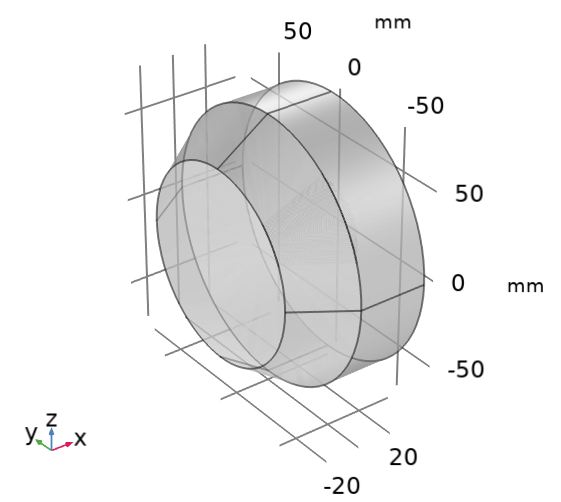
\includegraphics{../fig/fig_ConvNatComsol/Comsol_SimplifiedModel_Geometry5.png}
    \caption{Géométrie du modèle simplifié du régénérateur et de la cavité d'adaptation d'impédance.}
    \label{fig:Comsol_ModeleSimplifie_Geometrie}
\end{figure}

\subsection{Volume d'adaptation d'impédance}



\subsection{Régénérateur}
Le nombre de Rayleigh dans un matériau poreux dépend de sa perméabilité. Il est assez difficile de la calculer car il faut connaître la vitesse d'écoulement et la différence de pression de part et d'autre du domaine étudié. Le régénérateur est modélisé dans Comsol pour extraire ses paramètres hydrauliques et calculer les nombres adimensionnels déjà présentés.

De plus, cette simulation vise à vérifier l'hypothèse de superposition des effets thermiques. En effet, la distribution de température du côté de l'échangeur froid dans le cas de l'orientation `\texttt{H1}' laisse à penser que la température froide et constante sur la section provoqué par l'effet thermoacoustique, la conduction thermique dans le noyau qui provoque une différence de température entre le centre du noyau et sa périphérie, et la convection naturelle qui apporte un gradient de température selon la direction verticale se combinent.

Dans cette simulation, le régénérateur est modélisé en premier lieu comme un solide non poreux. Ainsi, il est possible de répondre à une question sur la présence ou non d'un flux moyen non nul de convection naturelle significatif à l'intérieur du noyau.

\section{Modèle temporel} \label{chap:ModeleTemporel}
Un modèle temporel du régime transitoire de la distribution axiale de température dans le noyau thermoacoustique est créé pour approcher le réfrigérateur \textsc{Tacot} d'après le modèle 1D développé par Lotton \textit{et al.} pour un réfrigérateur à ondes stationnaires \cite{lotton_transient_2009}. Ce modèle calcule le bilan de chaleur au sein du régénérateur en faisant intervenir les flux de chaleur thermoacoustique $Q_{\sf TA}$, de conduction thermique $Q_{\sf cond}$, de frottement visqueux $Q_{\sf visq}$, et de pertes latéral au travers des parois de la cavité $Q_{\sf lat}$ dans chaque volume élémentaire $S_{\sf reg} \deriv x$ du régénérateur discrétisé. Pour compenser les écarts entre les prévisions du modèle et les mesures, un flux de chaleur $Q_{\sf vort}$ estimé empiriquement est également pris en compte dans les conditions aux frontières sur l'axe du noyau. Ce flux est supposé lié aux effets de bord du noyau tels que la vorticité, les pertes de charges ou les effets entropiques. Ce modèle 2D prend en compte les conditions au limites suivantes : 



%\begin{comment}
Le modèle a pour but de calculer les transferts thermiques dans le régénérateur pour n'importe quel champ acoustique. Aussi, l'expression des quantités oscillantes dans le noyau peut-être donnée par un produit de matrices de transfert élémentaires de l'équation~\eqref{eq:TMatrix_prod_TppTuu}. Dans le cas d'un régénérateur compact du point de vue acoustique, les coefficients de cette matrice de transfert sont donnés par

\begin{subequations}
	\begin{multicols}{2}
	\noindent
	\begin{align}
		T_{pp}^{(n)} &= 1, \label{eq:TMatrix_Tpp_regen}\\
		T_{pu}^{(n)} &= -\frac{i \omega \rho}{\Phi S (1-f_\nu)}\deriv x, \label{eq:TMatrix_Tpu_regen}
		\end{align}
		\begin{align}
		T_{up}^{(n)} &= -\frac{i \omega \Phi S}{\gamma P_0} \deriv x, \label{eq:TMatrix_Tup_regen}\\
		T_{uu}^{(n)} &= 1. \label{eq:TMatrix_Tuu_regen}
	\end{align}
	\end{multicols}
	\label{eq:TMatrix_regen}
\end{subequations}

\subsection{Mécanismes pris en compte dans le modèle}
Ensuite, les flux thermiques sont également pour la plupart différents dans le cas d'un réfrigérateur contenant un régénérateur à la place d'un \textit{stack}, et sont définis dans les équations \eqref{eq:FluxTA_Lotton_Regen} à \eqref{eq:FluxLat_Lotton} accompagnées de la figure~\ref{fig:Schema_FluxThermiquesNoyau_Gaelle} pour les illustrer au sein du régénérateur.

\begin{figure}[!ht]
    \centering
    \external{fig_Schema_FluxThermiquesNoyau_Gaelle}
%    \externalremake
    \begin{tikzpicture}%[yscale=3]
	\def\Lreg{6cm};
	\def\Ryreg{4cm};
	\def\Rxreg{1cm};%{\Ryreg/3};
	\def\CHXnorth{0,\Ryreg};
	\def\CHXsouth{0,-\Ryreg};
	\def\AHXnorth{\Lreg,\Ryreg};
	\def\AHXsouth{\Lreg,-\Ryreg};
	

	


% --------------------------------------------------- Flux thermiques
%\fill[MatlabBlue,opacity=.5] (\CHXnorth) arc [start angle=90, end angle=270, x radius=\Rxreg, y radius=\Ryreg] -- cycle; % Face gauche (fond)
%\draw[very thick] (\CHXnorth) arc [start angle=90, end angle=270, x radius=\Rxreg, y radius=\Ryreg]; % Face gauche (contour)

\filldraw[fill=MatlabBlue, fill opacity=.5, draw=black,very thick] (\CHXnorth) rectangle (\AHXsouth);

%%% Q_vort
\foreach \y in {-.5,0,.5}{
\draw[arw,->,draw=MatlabPurple,line width=1mm] (-.1*\Rxreg,{(\y+.02)*\Ryreg}) -- ++(-\Rxreg,0) arc (-90:-360:.35);
\draw[arw,->,draw=MatlabPurple,line width=1mm] (-.1*\Rxreg,{(\y-.02)*\Ryreg}) -- ++(-\Rxreg,0) arc (90:360:.35);
\draw[arw,->,draw=MatlabPurple,line width=1mm] (\Lreg+.1*\Rxreg,{(\y+.02)*\Ryreg}) -- ++(\Rxreg,0) arc (-90:180:.35);
\draw[arw,->,draw=MatlabPurple,line width=1mm] (\Lreg+.1*\Rxreg,{(\y-.02)*\Ryreg}) -- ++(\Rxreg,0) arc (90:-180:.35);}

\draw (-1.2*\Rxreg,-.5*\Ryreg) node[left]{$\left.Q_{\sf vort}\right|_{x=0}$};
\draw (\Lreg+1.2*\Rxreg,.5*\Ryreg) node[right]{$\left.Q_{\sf vort}\right|_{x=L_{\sf reg}}$};

% --------------------------------------------------- Fond de schéma

\draw[dotted, ->, very thick] ({-3.5*\Rxreg},-\Ryreg) -- ({\Lreg+3.5*\Rxreg},-\Ryreg) node [right] {$\mathbf e_x$}; % axe x
%\fill[MatlabBlue,opacity=.5] (\CHXnorth) arc [start angle=90, end angle=-90, x radius=\Rxreg, y radius=\Ryreg] -- cycle; % bord gauche (moitié droite pour que l'axe x rentre "dans le noyau")
\draw[dotted, ->, very thick] ($(\CHXsouth)+(0,-.3*\Ryreg)$) -- ($(\CHXnorth)+(0,.3*\Ryreg)$) node [above] {$\mathbf e_r$}; % axe r

%\draw[dashed, very thick] (\AHXnorth) arc [start angle=90, end angle=270, x radius=\Rxreg, y radius=\Ryreg]; % paroi gauche arrière pointillée
%\filldraw[fill=MatlabBlue, fill opacity=.5, draw=black,very thick] (\CHXnorth) arc [start angle=90, end angle=-90, x radius=\Rxreg, y radius=\Ryreg] -- (\AHXsouth) arc [start angle=-90, end angle=90, x radius=\Rxreg, y radius=\Ryreg] --cycle; % Paroi du cylindre


% --------------------------------------------------- Dimensions
\draw (\CHXnorth) node [above right] {\begin{tabular}{ll}\'Echangeur \\  froid\end{tabular}};
\draw (\AHXnorth) node [above left] {\begin{tabular}{rr}\'Echangeur \\ ambiant \end{tabular}  };

\draw (0,-\Ryreg) node[below left] {0};
\draw (\Lreg,-\Ryreg) node{|} node[below left] {$L_{\sf reg}$};
\draw (\CHXnorth) -- ++(-.5cm,0) node[left] {$2 R_{\sf reg}$};

%%% Q_TA
\draw[arw,->,draw=MatlabBlue] ({.25*\Lreg},0) -- ++(.33*\Lreg,0) node[right] {$Q_{TA}$} node(MidQTA)[midway]{};
%
%\draw[arw,<-,draw=MatlabBlue] ($(\CHXsouth)+(-1mm,-1mm)$) -- ++(-120:.33*\Lreg)node[pos=.75, left]{$Q_{TA}(0)$};
%\draw[arw,->,draw=MatlabBlue] ($(\AHXsouth)+(1mm,-1mm)$) -- ++(-60:.33*\Lreg)node[pos=.25, right]{$Q_{TA}(L_{\sf reg})$};

%%% Q_cond
\draw[arw,->,draw=MatlabOrange] ({.75*\Lreg},.15*\Ryreg)  -- ++(-.33*\Lreg,0) node[left] {$Q_{\sf cond}^{(x)}$} node(MidCondx1)[midway]{};
\draw[arw,->,draw=MatlabOrange] ({.75*\Lreg},-.15*\Ryreg)  -- ++(-.33*\Lreg,0) node(MidCondx2)[midway]{} node[left] {$Q_{\sf cond}^{(x)}$};

\draw[arw,->,draw=MatlabYellow] ({.25*\Lreg},.3*\Ryreg)  -- ++(0,.33*\Lreg) node[above] {$Q_{\sf cond}^{(r)}$} node(MidCondr1)[midway]{};
\draw[arw,->,draw=MatlabYellow] ({.75*\Lreg},-.3*\Ryreg)  -- ++(0,-.33*\Lreg) node[below] {$Q_{\sf cond}^{(r)}$} node(MidCondr2)[midway]{};

%%% Q_visq
\draw[arw,<->,draw=PythonGreen] ($(MidCondr1 -| MidCondx1)+(-.33*\Lreg/2,0)$)  -- ++(.33*\Lreg,0) node[midway,above]{$Q_{\sf visq}$};
\draw[arw,<->,draw=PythonGreen] ($(MidCondr2 -| MidQTA)+(-.33*\Lreg/2,0)$)  -- ++(.33*\Lreg,0) node[midway,below]{$Q_{\sf visq}$};


%%% Q_lat
\draw[->,line width=1mm,decorate,decoration={snake,amplitude=.4mm,segment length=2mm,post length=2mm},red] (.5*\Lreg,1.1*\Ryreg) -- ++(0,1cm) node [above] {$\left.h_r\right|_{r=2R_{\sf reg}}\theta$};
\draw[->,line width=1mm,decorate,decoration={snake,amplitude=.4mm,segment length=2mm,post length=2mm},red] (.5*\Lreg,-1.1*\Ryreg) -- ++(0,-1cm) node [below] {$\left.h_r\right|_{r=0}\theta$};

%\draw[red] (.5*\Lreg,1.1*\Ryreg) node{$T_{paroi}$}; 
%\draw[red, line width=1mm] ($(\CHXnorth)+(0,0)$) -- ($(\AHXnorth)+(0,0)$);
%\draw[red] (.5*\Lreg,-1.1*\Ryreg) node{$T_{paroi}$};
%\draw[red, line width=1mm] ($(\CHXsouth)+(0,0)$) -- ($(\AHXsouth)+(0,0)$);

\draw[->,line width=1mm,decorate,decoration={snake,amplitude=.4mm,segment length=2mm,post length=2mm},red] (-2*\Rxreg,0) -- ++(-1cm,0) node [midway, above] {$\left.h_x\right|_{x=0}\theta$};
\draw[->,line width=1mm,decorate,decoration={snake,amplitude=.4mm,segment length=2mm,post length=2mm},red] (\Lreg+2*\Rxreg,0) -- ++(1cm,0) node [midway, above] {$\left.h_x\right|_{x=L_{\sf reg}}\theta$};

%%% Q_HX
%\draw[arw,<-,draw=gray] ($(\CHXsouth)+(1mm,-1mm)$) -- ++(-60:.33*\Lreg)node[pos=.75, right]{$Q_f$};
%\draw[arw,->,draw=gray!50!black] ($(\AHXsouth)+(-1mm,-1mm)$) -- ++(-120:.33*\Lreg)node[pos=.25, left]{$Q_a$};
\draw[arw,<-,draw=gray] ($(\CHXsouth)+(0,-5mm)$) -- ++(0,-.33*\Lreg)node[pos=.75, right]{$Q_f$};
\draw[arw,->,draw=gray!50!black] ($(\AHXsouth)+(0,-5mm)$) -- ++(0,-.33*\Lreg)node[pos=.25, left]{$Q_a$};

\end{tikzpicture}
    \caption{Représentation schématique des flux thermiques considérés dans le modèle transitoire du régénérateur.}
    \label{fig:Schema_FluxThermiquesNoyau_Gaelle}
\end{figure}

\begin{enumerate}[label=\textbf{(\roman*)}]
\item Tout d'abord, le flux thermoacoustique 1D est calculé avec l'équation~\eqref{eq:FluxTA_swift} développée par Swift \cite{swift_thermoacoustics_2017}

\begin{multline}
	Q_{TA} = \underbrace{ -\frac12~\RE\left[ \frac{ f_\kappa-f_\nu^* }{ (1+\mathrm{Pr})(1-f_\nu^*) } pu^* \right] }_{q_{TA}(x)} \\ 
	+ \overbrace{ \frac12 \frac{\rho_0 C_p}{\Phi S}~\IM\left[ \frac{f_\kappa + \mathrm{Pr} f_\nu^*}{(1-\mathrm{Pr}^2)|1-f_\nu|^2} \right] |u|^2 }^{k_{TA}(x)}\partial_x \theta(r,x;t),
\label{eq:FluxTA_Lotton_Regen}
\end{multline}
où $\theta(r,x;t) = T_0(r,x;t)-T_\infty$ est l'écart de la température locale à la température initiale. Pour la suite du document, cet écart de température sera simplement écrit $\theta$, sans la dépendance spatio-temporelle. Il est important de remarquer la partie réelle de ce flux thermique, notée $q_{TA}$, qui ne dépend que du champ acoustique, et la partie imaginaire $k_{TA}$ qui dépend du gradient de température le long du stack et qui peut être vu comme un terme de conduction induite par l'effet thermoacoustique.

\item Ensuite, la conduction dans le régénérateur est prise en compte dans les directions $\textbf e_x$ et $\textbf{e}_r$ du régénérateur avec l'équation exprimée en coordonnées cylindriques par

%\begin{equation}
%	Q_{\sf cond} = -\begin{pmatrix}
%	k_x\\
%	k_r\\
%	k_\alpha
%	\end{pmatrix} \cdot \nabla \theta,
%	\label{eq:FluxCond_Lotton}
%\end{equation}

\begin{equation}
	\left\{ \begin{aligned}
		Q_{\sf cond}^{(x)} &= -k_x \partial_x T\\
		Q_{\sf cond}^{(r)} &= -k_r \partial_r T \echaf{\text{ corriger expression avec gradient radial}}
	\end{aligned}\right.
	\label{eq:FluxCond_Lotton}
\end{equation}
avec les indices $x$ et $r$ dénotant respectivement les directions axiale et radiale où circulent les flux de conduction. La porosité influe sur la conductivité thermique apparente et $k_i~=~\Phi_i k_{g} + (1-\Phi_i)k_{s}$ ($i=x,r$). \echaf{En première aproximation, il est possible de considérer les valeurs de conductivité comme égales les unes aux autres. Cependant, c'est inexact car le long de l'axe $\mathbf e_x$ le milieu est constitué de l'empillement de tissus métalliques tandis que dans la direction $\mathbf e_r$ le flux de chaleur parcourt les fils qui forment le tissus en lui-même.}

%\begin{equation}
%Q_{\sf cond}^{(x)} = -k_x\partial_x\theta~\mathrm{\mathbf e_x},
%\label{eq:FluxCondx_Lotton}
%\end{equation}
%avec... 
%
%\begin{equation}
%Q_{\sf cond}^{(r)} = -k_r\partial_r\theta~\mathrm{\mathbf e_r},
%\label{eq:FluxCondr_Lotton}
%\end{equation}
%
%\begin{equation}
%Q_{\sf cond}^{(\alpha)} = -k_\alpha\partial_\alpha\theta~\mathrm{\mathbf e_\alpha},
%\label{eq:FluxCondalpha_Lotton}
%\end{equation}
%\textcolor{red}{Rassembler $Q_{cond}$ en 1 seul terme} avec ...

\item Les pertes visqueuses sont estimées avec l'équation

\begin{equation}
Q_{\sf visq} = \frac{1}{R_{\sf reg}^2} \int_{0}^{R_{\sf reg}} \frac{1}{\tau_0} \int_0^{\tau_0} \mu (\partial_r u)^2\ r \deriv r \deriv t.
\label{eq:FluxVisq_Lotton}
\end{equation}

En utilisant l'identité

\begin{equation*}
\frac{1}{T}\int_{0}^{\tau_0}\mu(\partial_r u)^2\deriv t = \frac12|\partial_r u|^2,
\end{equation*}
l'équation \eqref{eq:FluxVisq_Lotton} est réécrite comme

\begin{equation}
	Q_{\sf visq} = \frac{1}{2R_{\sf reg}^2} \int_{0}^{R_{\sf reg}} \mu |\partial_r u|^2\ r \deriv r
	\label{eq:FluxVisq_Lotton_IntegralTSimplifie}
\end{equation}

\echaf{poursuivre après simu}
dont l'intégrale sur la section de rayon $R_{\sf reg}$ est résolue par une méthode numérique.

\item Les effets de bords tels que les pertes de charges ou la vorticité sont pris en compte aux frontières du domaine grâce à des flux de chaleur $Q_{\sf vort}$ estimés empiriquement à $x=0$ et $x=L_{\sf reg}$.

\item Les pertes latérales aux extrémités en $x=0$ et $x=L_{\sf reg}$ du régénérateur sont prises en compte par

\begin{equation}
	Q_{\sf lat}^{(x)} = h_x \theta,
	\label{eq:FluxLat_Lotton}
\end{equation}
où $h_x$ est le coefficient d'échanges thermique entre les extrémités du noyau et le fluide à température ambiante. Ils sont déterminés de façon empirique.

%Alternativement, il est possible de prendre en compte les échanges de chaleur au bord et dans l'axe du noyau par un terme qui représente le flux de chaleur induit par les oscillations acoustiques noté $\psi_{ac}$ dans la thèse de Guédra \cite{guedra_etudes_2012} et défini par
%
%\begin{equation}
%	\psi_{ac}=\frac12 \rho_0 T_0 \RE[s v^*],
%	\label{eq:FluxChaleurAcou_Guedra}
%\end{equation}
%dont la moyenne sur la section s'écrit
%
%\begin{align}
%	\langle\psi_{ac}\rangle &= \RE[g]\mathcal I \IM[g]\mathcal J - k_{ac}\deriv_x T_0,	\label{eq:FluxChaleurAcou_Guedra_Moy}\\
%										&= \langle\psi_{ac,0}\rangle
%\end{align}


\item Les pertes latérales sur la périphérie à $r=R_{\sf reg}$ sont prises en comptes en considérant une température variant dans le temps et le long du régénérateur, déterminée par la méthode des transformations intégrales. Ce calcul, expliqué dans la section~\ref{chap:TransfoIntegrales}, est appliqué à un système présenté sur la figure~\ref{fig:TemperatureCanisterConditionLimite}, qui contient le \echaf{canister} dont l'épaisseur est considérée infinie pour le calcul numérique, insérée dans le tube en acier inoxydable qui contient le noyau, suivi du gaz contenu dans le canal de rétroaction.\echaf{continuer}

La séparation du calcul de la température de la paroi du reste de la simulation permet de résoudre analytiquement le problème, ce qui est impossible si le couplage entre ces systèmes est considéré. L'hypothèse de la longueur infinie du \echaf{canister} repose sur le fait que l'influence du \echaf{canister} sur le régénérateur prédomine \echaf{sur l'impact inverse}.


\begin{figure}[!ht]
    \centering
    \external{fig_TemperatureCanisterConditionLimite}
    %\externalremake
    \begin{tikzpicture}
	\def\lREG{3.9cm};
	\def\eCAN{5mm};
	\def\eWALL{13pt};
	\def\eFB{6mm};
	
	\fill[gray] (0,0) node(O){} rectangle (\lREG,-\eCAN);
	\fill[top color=gray,bottom color=white](0,-\eCAN) node(eCAN){} rectangle (\lREG,-2*\eCAN);
	
	\fill[right color=black!25,left color=white] ($(O)+(0,\eWALL)$) node(eWALL){} rectangle (-\lREG/4,0);
	\fill[black!25] (O) rectangle (\lREG,\eWALL) node[midway]{$k_{\sf acier}$};
	\fill[right color=white,left color=black!25] ($(O)+(\lREG,0)$) rectangle ++(\lREG/4,\eWALL);
	
	\fill[blue!25!white] ($(O)+(0,\eWALL+\eFB)$) node(eFB){} rectangle ++(\lREG,-\eFB);
	\fill[right color=blue!25!white,left color=white] (eFB) rectangle ++(-\lREG/4,-\eFB);
	\fill[right color=white,left color=blue!25!white] ($(eFB)+(\lREG,0)$) rectangle ++(\lREG/4,-\eFB);
	\fill[top color=white,bottom color=blue!25!white] (eFB) rectangle ++(\lREG,.5*\eFB);
	\shade[upper left=white,upper right=white,
         lower left=white,lower right=blue!25!white] (eFB) rectangle ++(-\lREG/4,.5*\eFB);
	\shade[upper left=white,upper right=white,
         lower left=blue!25!white,lower right=white] ($(eFB)+(\lREG,0)$) rectangle ++(\lREG/4,.5*\eFB);
	\draw[->,line width=.5mm,decorate,decoration={snake,amplitude=.4mm,segment length=2mm,post length=2mm},blue!75!white] ($(eWALL)+(\lREG/2,0)$) -- ++(0,\eFB) node[midway,right,blue!75!white]{$h_{\sf conv}$};
	
	
	
	\draw[->] ($(eFB)+(0,\eFB)$) -- ($(eCAN)+(0,-2.1*\eCAN)$) node[left]{$-\mathbf{e}_r$};
	\draw[->] (-1mm,0) node(lab){} -- (4*\lREG/3,0) node[above]{$\mathbf{e}_x$};
	
	\draw ($(eWALL) + (-\lREG/4,1.5*\eFB/2)$) node[left]{Canal de rétroaction};
	\draw ($(O) + (-\lREG/4,\eWALL/2)$) node[left]{Tube contenant le noyau};
	\draw (eWALL) node[left]{$e_{\sf wall}$};
	\draw (O) node[left]{0};
	\draw[line width=.5mm,dashed] (eCAN.base) node[left]{$e_{\sf can}$} -- ++(\lREG,0);
\end{tikzpicture}
    \caption{Géométrie équivalente pour établir la condition de température à la frontière $r=R_{\sf reg}$. \echaf{ajouter conductivité}}
    \label{fig:TemperatureCanisterConditionLimite}
\end{figure}

\item \echaf{Flux de chaleur apportés ou retirés par les échangeurs}

$Q=\epsilon Q_i$ avec 
\begin{equation}
	\epsilon = \frac{k_s k_{sfrac} (1-\Phi)S_{\sf reg}}{k_s k_{sfrac} (1-\Phi)S_{\sf reg} + k_{\sf can} S_{\sf can}}
\end{equation}
et $k_{sfrac}$ le facteur de dégradation de conductivité \cite{lewis_measurement_1998}

\end{enumerate}

\subsection{Bilan thermique}

Ces flux de chaleurs sont reportés dans l'équation modifiée du bilan de chaleur qui s'écrit

%\begin{equation}
%[\Phi\rho_0 C_p + (1-\Phi)\rho_s C_s]\partial_t \theta = - \nabla \cdot (Q_{TA} + Q_{\sf cond}) + Q_{\sf visq},
%\label{eq:BilanChaleur_LottonPoignand}
%\end{equation}
%ce qui donne après développement de l'opérateur divergence en coordonnées cylindrique,

\begin{equation}
[\Phi\rho_0 C_p + (1-\Phi)\rho_s C_s]\ \partial_t \theta = - \partial_x Q_{TA} - \partial_x Q_{\sf cond}^{(x)} - \frac{1}{r}\partial_r[r Q_{\sf cond}^{(r)}] + Q_{\sf visq}.
\label{eq:BilanChaleur_LottonPoignand_ApDvptCylin}
\end{equation}

Le premier membre désigne la variation d'énergie interne suite à la variation de température, et le second membre, l'expression des flux thermiques dans chaque volume élémentaire. D'une part, les flux thermoacoustiques et de conduction sont \og de passage \fg{} au travers de ce volume, et c'est seulement dans le cas d'une divergence non nulle que la température y évolue. D'autre part, les effets visqueux se produisent dans chaque volume, il sont donc source de chaleur et doivent être pris en compte tels quels. Ceci dit, le régénérateur est supposé axisymétrique, ce qui permet de considérer les composantes azimuthales $\nabla_\alpha \cdot Q_{TA}$ et $\nabla_\alpha \cdot Q_{\sf cond}$ comme nulles.

Le problème décrit par l'équation~\ref{eq:BilanChaleur_LottonPoignand_ApDvptCylin} est conditionné aux frontières en $x=0$, $x=L_{\sf reg}$ et $r=R_{\sf reg}$ pour respecter la conservation d'énergie. Ces conditions se traduisent par le système d'équations

\begin{subequations}
	\begin{align}
		Q_{\sf cond}^{(x)} + Q_f + Q_{\sf vort}(0) &= Q_{TA}(0) + h_x(0)\theta,\quad &x=0,\ r \in [0,R_{\sf reg}], t>0 \label{eq:CondFront_x_0Froid}\\%
		Q_{TA}(L_{reg}) + Q_{\sf vort}(L_{reg})  &= Q_{\sf cond}^{(x)} + Q_a + h_x(L_{\sf reg})\theta, \quad &x=L_{\sf reg},\ r \in [0,R_{\sf reg}], t>0 \label{eq:CondFront_x_LregAmb}\\%
		Q_{\sf cond}^{(r)} &= h_r(R_{\sf reg})\theta, \quad &r=R_{\sf reg},\ x \in [0,L_{\sf reg}], t>0 \label{eq:CondFront_r_ra}
	\end{align}%
	\label{eq:CondFront}%
\end{subequations}
où $Q_f$ et $Q_a$ sont les flux de chaleur retirés à l'échangeur froid d'une part et apporté à l'échangeur ambiant d'autre part. Ce système signifie que pour chaque frontière, la somme des flux entrant dans l'interface et des sources thermiques est égale aux flux qui en sortent. Il reste à introduire la distribution de température à $t=0$ notée $\theta_0(x,r)$ comme condition initiale, qui se présente comme

\begin{equation}
	\theta(x,r,t=0) = \theta_0(x,r).
	\label{eq:CondInit}
\end{equation}

Le report des flux de chaleurs des équations~\eqref{eq:FluxTA_Lotton_Regen} à \eqref{eq:FluxLat_Lotton} dans l'équation du problème~\eqref{eq:BilanChaleur_LottonPoignand_ApDvptCylin}, dans les conditions aux frontières~\eqref{eq:CondFront} et dans la condition initiale~\eqref{eq:CondInit} permet de poser le problème tel que

\begin{equation}
	toto
	\label{eq:ProbTransitoire_ApDvpt}
\end{equation}

\subsection{Méthode des transformations intégrales}\label{chap:TransfoIntegrales}
La résolution de l'équation~\eqref{eq:BilanChaleur_LottonPoignand_ApDvptCylin} qui comporte des termes sources requiert l'usage de la méthode des transformations intégrales après réécriture des équations du système sous la forme d'un problème homogène équivalent \cite{ozisik_heat_1993}. Les équations s'écrivent alors

\begin{subequations}
	\begin{align}
		\echaf{Systeme\ ici},\label{eq:1_LottonPoignand}\\
		\echaf{Systeme\ ici},\label{eq:2_LottonPoignand}
	\end{align}
	\label{eq:SystemeEq_LottonPoignand}
\end{subequations}
avec les changements de variables suivants

\begin{itemize} \color{red}
	\item 1
	\item 2.
\end{itemize}

%\end{comment}



\chapter{\'Etude experimentale}\label{chap:EtudeExpe}
\mylocaltoc

\section{Convection naturelle}\label{chap:EtudeExpe_ConvNat}
Lors des expériences réalisées lors de la caractérisation du réfrigérateur \textsc{Tacot}, il a été montré que le gradient axial de température dans le noyau thermoacoustique n'est pas linéaire, et que les températures ne sont pas homogènes le long de la direction transverse du noyau \textcolor{red}{figure ?}\cite{ramadan_design_2021}. Cet écart au comportement attendu, c'est-à-dire un gradient linéaire entre les côtés froid et ambiant du noyau thermoacoustique, ainsi qu'une température radiale uniforme sur la section du noyau thermoacoustique, implique la présence d'un écoulement moyen non nul et d'effets non-linéaires dans le réfrigérateur. Parmi les hypothèses formulées quant à la cause de ces disparités avec la théorie linéaire de Rott, plusieurs hypothèses peuvent être envisagées : vent acoustique, turbulence, formation de tourbillons, génération d'harmoniques supérieures, et convection naturelle. Parmi ces effets, peu d'études portent sur cette dernière, bien qu'il ait déjà été montré que le déclenchement de moteurs ou encore l'uniformité de température sur la section y étaient très sensibles \cite{ross_influence_2003,  hireche_numerical_2019, ramadan_experimental_2018,  zhang_novel_2011}.

\subsection{Dans la cavité conique entre la source acoustique principale et le noyau thermoacoustique}

Pour faciliter l'analyse de la distribution de température dans le noyau thermoacoustique et ses alentours, celui-ci est découpé en cinq zones réparties le long de l'axe $\mathbf{e}_x$.
La première étude concerne la distribution de température entre la source acoustique principale et l'échangeur froid, c'est-à-dire dans le cône d'adaptation d'impédance acoustique matérialisé en orange sur la figure~\ref{fig:SchemaGeneralTACOT}. Il est en effet initialement suspecté que la nature du gaz, les dimensions du volume dans lequel il se trouve et les conditions thermiques aux frontières permettent la mise en mouvement du fluide. Cette hypothèse est de plus appuyée par le calcul du nombre de Rayleigh $\mathrm{Ra}$ grâce à l'équation~\eqref{eq:NbrRayleigh}, et dont la valeur suffisament élevée \textcolor{red}{citation ?} est

\begin{equation}
%	\Rayleigh_{\Delta T=\qty{5}{\degreeCelsius}}=\num{2.4e6},
%	\label{eq:NbrRayleigh_Exple5K}
	\Rayleigh_{\Delta T=\qty{1}{\degreeCelsius}}=\num{4.7e5},
	\label{eq:NbrRayleigh_Exple1K}
\end{equation}  
ce qui correspond après application numérique des équation~\eqref{eq:VitesseReference_Rayleigh} aux ordres de grandeur des vitesses verticale $v_{ref}^{// \mathbf g}$ et horizontale $v_{ref}^{\perp \mathbf g}$  

\begin{subequations}
	\begin{align}
%		v_{\sf ref}^{// \mathbf g} &\sim \qty{3.4e-2}{\meter\per\second} \text{ et}	\label{eq:VitesseReferenceV_Rayleigh_Exple5K}\\
%		v_{\sf ref}^{\perp \mathbf g} &\sim \qty{8.6e-4}{\meter\per\second}.	\label{eq:VitesseReferenceH_Rayleigh_Exple5K}
		v_{\sf ref}^{// \mathbf g} &\sim \qty{4.97e-2}{\meter\per\second} \text{ et}	\label{eq:VitesseReferenceV_Rayleigh_Exple1K}\\
		v_{\sf ref}^{\perp \mathbf g} &\sim \qty{1.9e-3}{\meter\per\second}.	\label{eq:VitesseReferenceH_Rayleigh_Exple1K}
	\end{align}
	\label{eq:VitesseReference_Rayleigh_Exple5K}%
\end{subequations}
dans le cas d'une différence de température de \qty{1}{\degreeCelsius}, soit une différence de température bien plus faible que celles obtenus pour toutes les expériences. Cette différence de température apparaît après le démarrage du réfrigérateur, suite au refroidissement du côté froid du régénérateur et celui dans une moindre mesure --- voire inexistant --- de la source acoustique principale située en face, à l'autre extrémité du cône d'adaptation d'impédance.

Les quatre orientations présentées sur la figure~\ref{fig:OrientationCore} sont regroupées par deux, avec d'une part les orientations horizontales du \textsc{Tacot} `\texttt{H1}' et `\texttt{H2}' où $\psi_v=\ang{0}$ (sous-figures~\subref{fig:OrientationCore_H1} et \subref{fig:OrientationCore_H2}), et d'autre part les orientations verticales `\texttt{V1}' et `\texttt{V2}' pour lesquelles $\psi_v=\pm\ang{90}$ (sous-figures~\subref{fig:OrientationCore_V1} et \subref{fig:OrientationCore_V2}). Pour chacun de ces groupes, les résultats des expériences réalisées aux trois amplitudes décrites dans le paragraphe~§\ref{chap:MesureAvecAcou} sont présentés sur les figures~\ref{fig:HeatOnly_CHXout_H1H2} -- \ref{fig:Acou_CHXout_H1H2_High} et \ref{fig:HeatOnly_CHXout_V1V2} -- \ref{fig:Acou_CHXout_V1V2_High}, respectivement pour les orientations horizontales et verticales. Pour rappel, la temperature initiale de chaque thermocouple est soustraite dans toutes les mesures qui suivent. De plus, les mesures sont rognées de \qtyrange{0}{3500}{\second} pour que la définition du régime stationnaire soit la même pour tous les résultats (sauf dans le cas du \textsc{Tacot} horizontal à moyenne amplitude acoustique, où un problème d'acquisition contraint le découpage de \qtyrange{0}{2700}{\second}). Un rééchantillonnage à \qty{.1}{\hertz} est également appliqué aux mesures de températures pour limiter la dimension des fichiers de données.

\subsubsection{Expériences avec le réfrigérateur horizontal}
Pour rappel, le réfrigérateur est placé à l'horizontal dans ces expériences. Les notations suivantes sont introduites pour cette partie concernant les expériences `\texttt{H1}' et `\texttt{H2}' :

\begin{itemize}
\item l'axe du noyau thermoacoustique $\mathbf e_x$ est perpendiculaire à $\mathbf g$, et est donc noté $\mathbf e_x^{\perp \mathbf g}$ ;
\item la dimension transverse du noyau $\mathbf e_r$ est séparée en deux :
	\begin{itemize}
	\item d'une part, la dimension transverse colinéaire à la gravité qui est notée $\mathbf e_r^{// \mathbf g}$ ;
	\item d'autre part, la dimension transverse perpendiculaire à la gravité qui est notée $\mathbf e_r^{\perp \mathbf g}$.
	\end{itemize}
\end{itemize}

\paragraph{Sans acoustique}
Pour séparer les phénomènes physiques et les transferts thermiques mis en jeu à l'intérieur de la pompe à chaleur, des expériences sans acoustiques sont menées préalablement aux mesures pour lesquelles les sources acoustiques sont alimentées. Un gradient de température le long du noyau thermoacoustique est maintenu en appliquant un chauffage par les cartouches contenues dans l'échangeur de chaleur froid, et un écoulement d'eau à température ambiante dans l'échangeur de chaleur ambiant. Ainsi, dans la cavité considérée ici, l'échangeur froid agit comme une source de chaleur et la source acoustique reste à température ambiante, et la situation est en quelque sorte l'opposée des expériences avec acoustique. Les résultats du régime transitoire sont présentés sur la figure~\ref{fig:HeatOnly_CHXout_H1H2}. Il est possible de remarquer

\begin{figure}[!ht]
    \centering
    \external{fig_HeatOnly_CHXout_H1H2}
%    \externalremake
    \begin{tikzpicture}
    \def\width{.9*\textwidth};
    \def\height{.5*\width};
    \def\legx{.5cm};
    \def\legy{\legx};
    
    \begin{axis}[name=plot,width={\width},height={\height},grid=both,minor tick num=4,
    grid style={line width=.1pt, draw=gray!10},
    major grid style={line width=.2pt,draw=gray!50},
    xlabel={Temps $t$ [\unit{\s}]},
    ylabel={\'Ecart de température $T-T|_{t=0}$ [\unit{\degreeCelsius}]},
    xmin=0,xmax=600,
	ymin=-1,ymax=30,
    xtick={0,600,1200,1800,2400,3000,3500},%ytick={0,9.1120/100000,1.4452/10000,2.5/10000,5/10000,1/1000},
    domain=0:100,
    legend style = {at={(1.01,1.05)},anchor = north east,cells={align=right}},legend columns=3,
    ]
    	
		
    	
    	\addlegendimage{legend image with text=}
		\addlegendentry{}
		\addlegendimage{legend image with text={`\texttt{H1}'}}
		\addlegendentry{}
		\addlegendimage{legend image with text=`\texttt{H2}'} 
		\addlegendentry{}   
    
    	\addlegendimage{legend image with text=Source acoustique principale}
    	\addlegendentry{}
    	
    	\addplot[ultra thick,black] file {{../fig/fig_ConvNat_HeatOnly/data/H1H2/data_TC0_0beg_RixOff_PhaseRIXHP-60°_OrientationH1_Qc61W_Serie1.txt}};\addlegendentry{}
		\addplot[ultra thick,black,dashed] file {{../fig/fig_ConvNat_HeatOnly/data/H1H2/data_TC0_0beg_RixOff_PhaseRIXHP-60°_OrientationH2_Qc61W_Serie1.txt}};\addlegendentry{}
		
		\addlegendimage{legend image with text=TC 1}
		\addlegendentry{}
		
    	\addplot[ultra thick,MatlabBlue] file {{../fig/fig_ConvNat_HeatOnly/data/H1H2/data_TC1_0beg_RixOff_PhaseRIXHP-60°_OrientationH1_Qc61W_Serie1.txt}};\addlegendentry{}
    	\addplot[ultra thick,MatlabBlue,dashed] file {{../fig/fig_ConvNat_HeatOnly/data/H1H2/data_TC1_0beg_RixOff_PhaseRIXHP-60°_OrientationH2_Qc61W_Serie1.txt}};\addlegendentry{}
    	
    	\addlegendimage{legend image with text=TC 2}
		\addlegendentry{}
		
    	\addplot[ultra thick,MatlabOrange] file {{../fig/fig_ConvNat_HeatOnly/data/H1H2/data_TC2_0beg_RixOff_PhaseRIXHP-60°_OrientationH1_Qc61W_Serie1.txt}};\addlegendentry{}
    	\addplot[ultra thick,MatlabOrange,dashed] file {{../fig/fig_ConvNat_HeatOnly/data/H1H2/data_TC2_0beg_RixOff_PhaseRIXHP-60°_OrientationH2_Qc61W_Serie1.txt}};\addlegendentry{}
    	
		\addlegendimage{legend image with text=TC 3}
		\addlegendentry{}
		
    	\addplot[ultra thick,MatlabYellow] file {{../fig/fig_ConvNat_HeatOnly/data/H1H2/data_TC3_0beg_RixOff_PhaseRIXHP-60°_OrientationH1_Qc61W_Serie1.txt}};\addlegendentry{}    	
    	\addplot[ultra thick,MatlabYellow,dashed] file {{../fig/fig_ConvNat_HeatOnly/data/H1H2/data_TC3_0beg_RixOff_PhaseRIXHP-60°_OrientationH2_Qc61W_Serie1.txt}};\addlegendentry{}
        
%        \legend{\\ \\};
    \end{axis}
    
%    \draw (plot.center) node[rotate=30]{\color{red}AFFICHER LES DONNEES};
\end{tikzpicture}
    \caption{\'Evolution temporelle des températures dans la cavité d'adaptation d'impédance pour les expériences dans les orientation `\texttt{H1}' et `\texttt{H2}' à \textit{drive ratio} nul.}
    \label{fig:HeatOnly_CHXout_H1H2}
\end{figure}

\paragraph{Avec acoustique}\label{chap:Acou_CHXout_H1H2_low}
Les premiers résultats sont obtenus pour les expériences horizontales `\texttt{H1}' et `\texttt{H2}' présentées sur les figures~\ref{fig:OrientationCore_H1} et \subref{fig:OrientationCore_H2}, à faible amplitude acoustique avec un \textit{drive ratio} $DR=\qty{.4}{\percent}$, et la température $\theta$ est tracée en fonction du temps $t$ sur la figure~\ref{fig:Acou_CHXout_H1H2_Low}. Pour les deux séries de mesures, c'est-à-dire les plans de thermocouples placés la verticale et l'horizontale et représentées respectivement en trait plein et trait tireté, la différence de température de \qty{2}{\degreeCelsius} entre le centre de l'échangeur froid et la source acoustique plus chaude apparaît après le démarrage de la pompe à chaleur à $t=\qty{100}{\second}$. Sur l'expérience réalisée dans l'orientation `\texttt{H2}', tous les thermocouples sont à la même altitude, et l'égalité des thermocouples~1~et~3 en bleu et en jaune permet notamment de visualiser une symétrie par rapport à un plan vertical passant par l'axe de symétrie du réfrigérateur. En revanche, cette symétrie n'est pas visible sur les courbes en traits pleins qui tracent les résultats de l'expérience menée en plaçant le réfrigérateur dans l'orientation `\texttt{H1}', puisqu'une dépendance de $\theta$ en fonction de $r$ est observable. En particulier, la courbe jaune correspondant au thermocouple~3 est la plus basse, en altitude comme en température, tandis que la courbe bleue qui représente le thermocouple~1 est la plus élevée des température mesurées sur l'échangeur froid, tout en y étant placée au plus haut. Toutefois, ce gradient de température n'est pas linéaire car la température au centre de l'échangeur froid mesurée par le thermocouple~2 n'est séparée que de \qty{.3}{\degreeCelsius} de la température mesurée par le thermocouple~3, tandis que cet écart est de \qty{2.5}{\degreeCelsius} avec le thermocouple~1. Cet dissymétrie est \textit{a priori} inattendue avec les résultats déjà obtenus dans les expériences sans acoustique.
\smallskip

%Tout d'abord, il est important de remarquer l'apparition de la différence de température après le démarrage du réfrigérateur entre la source acoustique principale (en noir) et le thermocouple 2 (en orange) situé en face, et ce, quel que soit l'orientation du plan de thermocouple. À cette différence de température s'ajoute la différence entre les courbes dans l'une et l'autre orientation, ce qui valide l'hypothèse de l'influence de la direction de la gravité sur la distribution de température dans la cavité d'adaptation d'impédance proposée par l'étude du nombre de Rayleigh. Notamment, la courbe jaune, qui représente la température mesurée par le thermocouple~3, atteint la température la plus faible quand ce capteur se trouve à la position la plus basse (courbe en trait plein), alors que lorsqu'il est à la même altitude que les autres thermocouples (courbe en trait tireté), il est également à la même température que le thermocouple~1. Un plan de symétrie vertical semble donc être présent lorsque le réfrigérateur est en position horizontale, ce qui est visible dans les expériences où les thermocouples sont sur un plan horizontal. En revanche, en vertical on s'attend à avoir un gradient linéaire mais en fait bof (comparer avec résultats lisn)

\begin{figure}[!ht]
    \centering
    \external{fig_Acou_CHXout_H1H2_Low}
%    \externalremake
    \begin{tikzpicture}
    \def\width{.9*\textwidth};
    \def\height{.5*\width};
    \def\legx{.5cm};
    \def\legy{\legx};
    
    \begin{axis}[width={\width},height={\height},grid=both,minor tick num=4,
    grid style={line width=.1pt, draw=gray!10},
    major grid style={line width=.2pt,draw=gray!50},
    xlabel={Temps $t$ [\unit{\s}]},
    ylabel={\'Ecart de température $\tau$ [\unit{\degreeCelsius}]},
    xmin=0,xmax=3500,
	ymin=-3,ymax=2,
    xtick={0,600,1200,1800,2400,3000,3500},%ytick={},
    domain=0:100,
    legend style = {at={(1.01,1.05)},anchor = north east,cells={align=right}},legend columns=3,
%    legend cell align=right
    ]
    
		\addlegendimage{legend image with text=}
		\addlegendentry{}
		\addlegendimage{legend image with text=H1}
		\addlegendentry{}
		\addlegendimage{legend image with text=H2} 
		\addlegendentry{}   
    
    	\addlegendimage{legend image with text=Source acoustique principale}
    	\addlegendentry{}
    	
    	\addplot[ultra thick,black] file {{../fig/fig_ConvNat_Acou/data/DataMatTxtH1H2Low/data_TC0_0beg_RixLow_PhaseRIXHP-60°_OrientationH1_Qc0W_Serie1.txt}};\addlegendentry{}%\addlegendentry{TC src. ac. 1 (H1)}
		\addplot[ultra thick,black,dashed] file {{../fig/fig_ConvNat_Acou/data/DataMatTxtH1H2Low/data_TC0_0beg_RixLow_PhaseRIXHP-60°_OrientationH2_Qc0W_Serie1.txt}};\addlegendentry{}%\addlegendentry{TC src. ac. 1 (H2)}
		
		\addlegendimage{legend image with text=TC 1}
		\addlegendentry{}
		
    	\addplot[ultra thick,MatlabBlue] file {{../fig/fig_ConvNat_Acou/data/DataMatTxtH1H2Low/data_TC1_0beg_RixLow_PhaseRIXHP-60°_OrientationH1_Qc0W_Serie1.txt}};\addlegendentry{}
    	\addplot[ultra thick,MatlabBlue,dashed] file {{../fig/fig_ConvNat_Acou/data/DataMatTxtH1H2Low/data_TC1_0beg_RixLow_PhaseRIXHP-60°_OrientationH2_Qc0W_Serie1.txt}};\addlegendentry{}
    	
		\addlegendimage{legend image with text=TC 2}
		\addlegendentry{}   	
    	
    	\addplot[ultra thick,MatlabOrange] file {{../fig/fig_ConvNat_Acou/data/DataMatTxtH1H2Low/data_TC2_0beg_RixLow_PhaseRIXHP-60°_OrientationH1_Qc0W_Serie1.txt}};\addlegendentry{}
    	\addplot[ultra thick,MatlabOrange,dashed] file {{../fig/fig_ConvNat_Acou/data/DataMatTxtH1H2Low/data_TC2_0beg_RixLow_PhaseRIXHP-60°_OrientationH2_Qc0W_Serie1.txt}};\addlegendentry{}
    	
    	\addlegendimage{legend image with text=TC 3}
    	\addlegendentry{}
    	
    	\addplot[ultra thick,MatlabYellow] file {{../fig/fig_ConvNat_Acou/data/DataMatTxtH1H2Low/data_TC3_0beg_RixLow_PhaseRIXHP-60°_OrientationH1_Qc0W_Serie1.txt}};\addlegendentry{}    	
    	\addplot[ultra thick,MatlabYellow,dashed] file {{../fig/fig_ConvNat_Acou/data/DataMatTxtH1H2Low/data_TC3_0beg_RixLow_PhaseRIXHP-60°_OrientationH2_Qc0W_Serie1.txt}};\addlegendentry{}
        
%        \legend{\\ \\};
    \end{axis}
\end{tikzpicture}
    \caption{\'Evolution temporelle des températures dans la cavité d'adaptation d'impédance pour les expériences dans les orientations `\texttt{H1}' et `\texttt{H2}' à faible \textit{drive ratio} $DR=\qty{.4}{\percent}$.}
    \label{fig:Acou_CHXout_H1H2_Low}
\end{figure}

La figure~\ref{fig:Acou_CHXout_H1H2_Mid} représente également l'évolution temporelle de la température $\theta$ dans la cavité, pour l'amplitude acoustique dite \og moyenne \fg{}  de \textit{drive ratio} $DR=\qty{2}{\percent}$. Après l'apparition de l'écart de température échangeur froid - source acoustique, qui vaut \qty{10.2}{\degreeCelsius} en `\texttt{H1}' et \qty{15.2}{\degreeCelsius} en `\texttt{H2}', des symptômes similaires à l'expérience à faible amplitude sont observables. À nouveau, les thermocouples~1~et~3 affichent des températures égales quand leurs altitudes sont égales (orientation `\texttt{H2}') et la symétrie des températures par rapport au plan vertical qui passe par le centre du noyau thermoacoustique est à nouveau mise en évidence. En revanche,  un écart de \qty{10}{\degreeCelsius} est visible lorsqu'ils sont l'un au dessus de l'autre (orientation `\texttt{H1}'). Dans cette orientation, le gradient vertical de température n'est toujours pas linéaire, puisque les températures~2~et~3 sont égales l'une à l'autre, \qty{10.2}{\degreeCelsius} en deça de la température mesurée par le thermocouple~1. 
\smallskip 

\begin{figure}[!ht]
    \centering
    \external{fig_Acou_CHXout_H1H2_Mid}
%    \externalremake
    \begin{tikzpicture}
    \def\width{.9*\textwidth};
    \def\height{.5*\width};
    \def\legx{.5cm};
    \def\legy{\legx};
    
    \begin{axis}[width={\width},height={\height},grid=both,minor tick num=4,
    grid style={line width=.1pt, draw=gray!10},
    major grid style={line width=.2pt,draw=gray!50},
    xlabel={Temps $t$ [\unit{\s}]},
    ylabel={\'Ecart de température $\tau$ [\unit{\degreeCelsius}]},
    xmin=0,xmax=2700,
	 ymin=-25,ymax=10,
    xtick={0,600,1200,1800,2400,2700},%ytick={0,9.1120/100000,1.4452/10000,2.5/10000,5/10000,1/1000},
    domain=0:100,
    legend style = {at={(1.01,1.05)},anchor = north east,rounded corners},legend columns=3,
%    legend cell align={right},
    ]
    
    	\addlegendimage{legend image with text=}
		\addlegendentry{}
		\addlegendimage{legend image with text=`\texttt{H1}'}
		\addlegendentry{}
		\addlegendimage{legend image with text=`\texttt{H2}'} 
		\addlegendentry{}   
    
    	\addlegendimage{legend image with text=TC 0}
    	\addlegendentry{}
    	
    	\addplot[ultra thick,black] file {{../fig/fig_ConvNat_Acou/data/DataMatTxtH1H2Mid/data_TC0_0beg_RixMid_PhaseRIXHP-60°_OrientationH1_Qc0W_Serie1.txt}};\addlegendentry{}
		\addplot[ultra thick,black,dashed] file {{../fig/fig_ConvNat_Acou/data/DataMatTxtH1H2Mid/data_TC0_0beg_RixMid_PhaseRIXHP-60°_OrientationH2_Qc0W_Serie1.txt}};\addlegendentry{}
		
		\addlegendimage{legend image with text=TC 1}
		\addlegendentry{}
		
    	\addplot[ultra thick,MatlabBlue] file {{../fig/fig_ConvNat_Acou/data/DataMatTxtH1H2Mid/data_TC1_0beg_RixMid_PhaseRIXHP-60°_OrientationH1_Qc0W_Serie1.txt}};\addlegendentry{}
    	\addplot[ultra thick,MatlabBlue,dashed] file {{../fig/fig_ConvNat_Acou/data/DataMatTxtH1H2Mid/data_TC1_0beg_RixMid_PhaseRIXHP-60°_OrientationH2_Qc0W_Serie1.txt}};\addlegendentry{}
    	
    	\addlegendimage{legend image with text=TC 2}
		\addlegendentry{}
		
    	\addplot[ultra thick,MatlabOrange] file {{../fig/fig_ConvNat_Acou/data/DataMatTxtH1H2Mid/data_TC2_0beg_RixMid_PhaseRIXHP-60°_OrientationH1_Qc0W_Serie1.txt}};\addlegendentry{}
    	\addplot[ultra thick,MatlabOrange,dashed] file {{../fig/fig_ConvNat_Acou/data/DataMatTxtH1H2Mid/data_TC2_0beg_RixMid_PhaseRIXHP-60°_OrientationH2_Qc0W_Serie1.txt}};\addlegendentry{}
    	
    	\addlegendimage{legend image with text=TC 3}
		\addlegendentry{}
		
    	\addplot[ultra thick,MatlabYellow] file {{../fig/fig_ConvNat_Acou/data/DataMatTxtH1H2Mid/data_TC3_0beg_RixMid_PhaseRIXHP-60°_OrientationH1_Qc0W_Serie1.txt}};\addlegendentry{}    	
    	\addplot[ultra thick,MatlabYellow,dashed] file {{../fig/fig_ConvNat_Acou/data/DataMatTxtH1H2Mid/data_TC3_0beg_RixMid_PhaseRIXHP-60°_OrientationH2_Qc0W_Serie1.txt}};\addlegendentry{}
        
%        \legend{\\ \\};
    \end{axis}
\end{tikzpicture}
    \caption{\'Evolution temporelle des températures dans la cavité d'adaptation d'impédance pour les expériences dans les orientations `\texttt{H1}' et `\texttt{H2}' à \textit{drive ratio} intermédiaire $DR~=~\qty{2}{\percent}$.}
    \label{fig:Acou_CHXout_H1H2_Mid}
\end{figure}

L'évolution de température $\theta$ au cours de l'expérience à l'amplitude acoustique \og élevée \fg{} est représentée sur la figure~\ref{fig:Acou_CHXout_H1H2_High}. Dans cette expérience, le \textit{drive ratio} est $DR=\qty{3.5}{\percent}$, ce qui correspond à l'amplitude pour laquelle les meilleures performances avaient été obtenues pour cette machine dotée du précédent noyau thermoacoustique. Les résultats de cette expérience sont assez similaire à ceux obtenus pour les faible et moyenne amplitude, à quelques différences près. Après l'établissement de la différence de température de \qty{16}{\degreeCelsius} entre le centre de l'échangeur froid et la source acoustique principale suite au démarrage de la machine, plusieurs effets sont à noter. Premièrement, la distribution de température est bien différente entre le cas `\texttt{H1}' où le plan de thermocouples est vertical et le cas `\texttt{H2}' où il est horizontal. En particulier, les courbes noires d'une part et les courbes rouges d'autre part se superposent d'une orientation à l'autre, ce qui est un effet attendu au vu de leur position sur l'axe de symétrie du réfrigérateur. Ensuite, la température le long de la dimension verticale $\mathbf e_r^{//\mathbf g}$ augmente avec cette dernière, encore une fois avec les thermocouples~2~et~3 à \qty{2}{\degreeCelsius} l'un de l'autre, et le thermocouple~1 \qty{12}{\degreeCelsius} au-dessus. Contrairement aux observations précédentes de ce gradient, à cette amplitude c'est le thermocouple~2 qui indique la température la plus basse, bien qu'il se trouve \qty{74}{\milli\meter} au-dessus du thermocouple~3. Cela dit, cet écart entre les deux thermocouples~2~et~3 est faible devant la valeur de température atteinte lors du fonctionnement de la machine et du refroidissement de cette zone, c'est-à-dire \qty{-23}{\degreeCelsius}. Il est possible de considérer cet écart comme une incertitude de mesure et ainsi se ramener à une analyse équivalente à celles des amplitudes plus faibles. Dans l'orientation `\texttt{H2}', la symétrie par rapport au plan vertical qui était visible aux amplitudes faibles et moyennes ne l'est plus. Les thermocouples~1~et~3 ne sont plus égaux, et sont séparés de \qty{2}{\degreeCelsius}. Cependant, pour les mêmes raisons que précédemment, l'écart est à nouveau considéré comme négligeable devant la valeur de la température atteinte, et les mêmes analyses qu'aux amplitudes faible et moyenne sont proposées.

\begin{figure}[!ht]
    \centering
    \external{fig_Acou_CHXout_H1H2_High}
%    \externalremake
    \begin{tikzpicture}
    \def\width{.9*\textwidth};
    \def\height{.5*\width};
    \def\legx{.5cm};
    \def\legy{\legx};
    
    \begin{axis}[width={\width},height={\height},grid=both,minor tick num=4,
    grid style={line width=.1pt, draw=gray!10},
    major grid style={line width=.2pt,draw=gray!50},
    xlabel={Temps $t$ [\unit{\s}]},
    ylabel={\'Ecart de température $\tau$ [\unit{\degreeCelsius}]},
    xmin=0,xmax=3500,
	 ymin=-30,ymax=10,
    xtick={0,600,1200,1800,2400,3000,3500},%ytick={0,9.1120/100000,1.4452/10000,2.5/10000,5/10000,1/1000},
    domain=0:100,
    legend style = {at={(1.01,1.05)},anchor = north east,rounded corners},legend columns=3,
%    legend cell align={right},
    ]
    	
    	\addlegendimage{legend image with text=}
		\addlegendentry{}
		\addlegendimage{legend image with text=`\texttt{H1}'}
		\addlegendentry{}
		\addlegendimage{legend image with text=`\texttt{H2}'} 
		\addlegendentry{}   
    
    	\addlegendimage{legend image with text=TC 0}
    	\addlegendentry{}
    	
    	\addplot[ultra thick,black] file {{../fig/fig_ConvNat_Acou/data/DataMatTxtH1H2High/data_TC0_0beg_RixHigh_PhaseRIXHP-60°_OrientationH1_Qc0W_Serie1.txt}};\addlegendentry{}
		\addplot[ultra thick,black,dashed] file {{../fig/fig_ConvNat_Acou/data/DataMatTxtH1H2High/data_TC0_0beg_RixHigh_PhaseRIXHP-60°_OrientationH2_Qc0W_Serie1.txt}};\addlegendentry{}
		
		\addlegendimage{legend image with text=TC 1}
		\addlegendentry{}
		
    	\addplot[ultra thick,MatlabBlue] file {{../fig/fig_ConvNat_Acou/data/DataMatTxtH1H2High/data_TC1_0beg_RixHigh_PhaseRIXHP-60°_OrientationH1_Qc0W_Serie1.txt}};\addlegendentry{}
    	\addplot[ultra thick,MatlabBlue,dashed] file {{../fig/fig_ConvNat_Acou/data/DataMatTxtH1H2High/data_TC1_0beg_RixHigh_PhaseRIXHP-60°_OrientationH2_Qc0W_Serie1.txt}};\addlegendentry{}
    	
    	\addlegendimage{legend image with text=TC 2}
		\addlegendentry{}
		
    	\addplot[ultra thick,MatlabOrange] file {{../fig/fig_ConvNat_Acou/data/DataMatTxtH1H2High/data_TC2_0beg_RixHigh_PhaseRIXHP-60°_OrientationH1_Qc0W_Serie1.txt}};\addlegendentry{}
    	\addplot[ultra thick,MatlabOrange,dashed] file {{../fig/fig_ConvNat_Acou/data/DataMatTxtH1H2High/data_TC2_0beg_RixHigh_PhaseRIXHP-60°_OrientationH2_Qc0W_Serie1.txt}};\addlegendentry{}
    	
		\addlegendimage{legend image with text=TC 3}
		\addlegendentry{}
		
    	\addplot[ultra thick,MatlabYellow] file {{../fig/fig_ConvNat_Acou/data/DataMatTxtH1H2High/data_TC3_0beg_RixHigh_PhaseRIXHP-60°_OrientationH1_Qc0W_Serie1.txt}};\addlegendentry{}    	
    	\addplot[ultra thick,MatlabYellow,dashed] file {{../fig/fig_ConvNat_Acou/data/DataMatTxtH1H2High/data_TC3_0beg_RixHigh_PhaseRIXHP-60°_OrientationH2_Qc0W_Serie1.txt}};\addlegendentry{}
        
%        \legend{\\ \\};
    \end{axis}
\end{tikzpicture}
    \caption{\'Evolution temporelle des températures dans la cavité d'adaptation d'impédance pour les expériences dans les orientations `\texttt{H1}' et `\texttt{H2}' à haut \textit{drive ratio} $DR=\qty{3.4}{\percent}$.}
    \label{fig:Acou_CHXout_H1H2_High}
\end{figure}


\subsubsection{Expériences avec le réfrigérateur vertical}
\paragraph{Sans acoustique}
\textcolor{red}{ICI les manips heat only}

\begin{figure}[!ht]
    \centering
    \external{fig_HeatOnly_CHXout_V1V2}
%    \externalremake
    \begin{tikzpicture}
    \def\width{.9*\textwidth};
    \def\height{.5*\width};
    \def\legx{.5cm};
    \def\legy{\legx};
    
    \begin{axis}[name=plot,width={\width},height={\height},grid=both,minor tick num=4,
    grid style={line width=.1pt, draw=gray!10},
    major grid style={line width=.2pt,draw=gray!50},
    xlabel={Temps $t$ [\unit{\s}]},
    ylabel={\'Ecart de température $T-T_i$ [\unit{\degreeCelsius}]},
    xmin=0,xmax=3500,
%	ymin=-6,ymax=4,
    xtick={0,600,...,3500},%ytick={0,9.1120/100000,1.4452/10000,2.5/10000,5/10000,1/1000},
    domain=0:100,
    legend style = {at={(1.01,1.05)},anchor = north east,cells={align=right}},legend columns=3,
    ]
    	
    	
    	\addlegendimage{legend image with text=}
		\addlegendentry{}
		\addlegendimage{legend image with text={`\texttt{V1}'}}
		\addlegendentry{}
		\addlegendimage{legend image with text=`\texttt{V2}'} 
		\addlegendentry{}   
    
    	\addlegendimage{legend image with text=Source acoustique principale}
    	\addlegendentry{}
    	
    	\addplot[ultra thick,black] file {{../fig/fig_ConvNat_HeatOnly/data/FixedPower/V1V2/data_TC0_0beg_RixOff_PhaseRIXHP-60°_OrientationV1_Qc40W_Serie1.txt}};\addlegendentry{}
		\addplot[ultra thick,black,dashed] file {{../fig/fig_ConvNat_HeatOnly/data/FixedPower/V1V2/data_TC0_0beg_RixOff_PhaseRIXHP-60°_OrientationV2_Qc40W_Serie1.txt}};\addlegendentry{}
		
		\addlegendimage{legend image with text=TC 1}
		\addlegendentry{}
		
    	\addplot[ultra thick,MatlabBlue] file {{../fig/fig_ConvNat_HeatOnly/data/FixedPower/V1V2/data_TC1_0beg_RixOff_PhaseRIXHP-60°_OrientationV1_Qc40W_Serie1.txt}};\addlegendentry{}
    	\addplot[ultra thick,MatlabBlue,dashed] file {{../fig/fig_ConvNat_HeatOnly/data/FixedPower/V1V2/data_TC1_0beg_RixOff_PhaseRIXHP-60°_OrientationV2_Qc40W_Serie1.txt}};\addlegendentry{}
    	
    	\addlegendimage{legend image with text=TC 2}
		\addlegendentry{}
		
    	\addplot[ultra thick,MatlabOrange] file {{../fig/fig_ConvNat_HeatOnly/data/FixedPower/V1V2/data_TC2_0beg_RixOff_PhaseRIXHP-60°_OrientationV1_Qc40W_Serie1.txt}};\addlegendentry{}
    	\addplot[ultra thick,MatlabOrange,dashed] file {{../fig/fig_ConvNat_HeatOnly/data/FixedPower/V1V2/data_TC2_0beg_RixOff_PhaseRIXHP-60°_OrientationV2_Qc40W_Serie1.txt}};\addlegendentry{}
    	
		\addlegendimage{legend image with text=TC 3}
		\addlegendentry{}
		
    	\addplot[ultra thick,MatlabYellow] file {{../fig/fig_ConvNat_HeatOnly/data/FixedPower/V1V2/data_TC3_0beg_RixOff_PhaseRIXHP-60°_OrientationV1_Qc40W_Serie1.txt}};\addlegendentry{}    	
    	\addplot[ultra thick,MatlabYellow,dashed] file {{../fig/fig_ConvNat_HeatOnly/data/FixedPower/V1V2/data_TC3_0beg_RixOff_PhaseRIXHP-60°_OrientationV2_Qc40W_Serie1.txt}};\addlegendentry{}
		
        
%        \legend{\\ \\};
    \end{axis}
%    \draw (plot.center) node[rotate=30]{\color{red}AFFICHER LES DONNEES};
\end{tikzpicture}
    \caption{\'Evolution temporelle des températures dans la cavité d'adaptation d'impédance pour les expériences dans les orientations `\texttt{V1}' et `\texttt{V2}' à \textit{drive ratio} nul.}
    \label{fig:HeatOnly_CHXout_V1V2}
\end{figure}

\paragraph{Avec acoustique}
La figure~\ref{fig:Acou_CHXout_V1V2_Low} trace les températures mesurées dans la cavité d'adaptation d'impédance pour des expériences où le réfrigérateur est placé dans les orientations verticales présentées figures~\ref{fig:OrientationCore_V1} et \subref{fig:OrientationCore_V2}, pour une amplitude \og faible \fg{} soit un \textit{drive ratio} $DR=\qty{.4}{\percent}$. Contrairement aux expériences horizontales où les effets de convection naturelle sont toujours présents mais pas toujours visibles, dans les expériences verticales il existe une configuration favorable à la mise en place d'une instabilité de convection naturelle de type Rayleigh-Bénard, et l'autre, inverse, qui est stable. La première configuration est l'orientation `\texttt{V1}', car la source acoustique y est en dessous du noyau thermoacoustique, car le sens du gradient de température est opposé à la gravité, tandis que la seconde est l'orientation `\texttt{V2}' où la source acoustique est au-dessus du noyau. Dans cette dernière orientation, le gradient de température est dans le même sens que la gravité, et il n'y a pas de flux de chaleur qui apparaît de manière spontanée. La première remarque concerne la différence d'aspect de l'évolution des températures entre une orientation et l'autre, malgré une axi-symétrie visible dans les deux cas et attendue au vu de la colinéarité de la dimensions axiale $\mathbf e_x$ et de la gravité $\mathbf g$. En observant les tracés en lignes tiretées, qui tracent l'évolution de la température $\theta$ au cours de l'expérience dans l'orientation `\texttt{V2}', une différence de température de \qty{3.2}{\degreeCelsius} entre l'échangeur froid du noyau et la source acoustique principale plus chaude apparaît et se maintient durant toute la durée de l'expérience. C'est d'ailleurs le plus grand écart de température relevé dans cette zone. Plus précisément, la température mesurée devant la source acoustique principale baisse \qty{.8}{\degreeCelsius} même après démarrage de celle-ci, ce qui est assez faible pour être en accord avec l'hypothèse de stabilité des températures en l'absence de flux massique causé par la convection naturelle. Dans l'orientation inverse `\texttt{V1}' représentée par les tracés en traits pleins, la différence de température apparaît également après le démarrage des sources acoustiques. Toutefois, après \qty{1800}{\second} les thermocouples sur l'axe de symétrie et en vis à vis l'un de l'autre, autrement dit devant la source acoustique principale et le thermocouple~2, affichent la même température. De manière plus générale, tous les thermocouple de cette zone d'adaptation d'impédance sont à des températures plus homogènes, puisque l'écart maximum de températures est dans ce cas de \qty{.8}{\degreeCelsius}. Un effet très remarquable pour cette orientation est l'évolution de température en deux étapes : la première, pendant laquelle la température sur l'échangeur froid diminue et qui s'étend du démarrage des sources à \qty{1100}{\second}, et la seconde, de cet instant jusqu'à la fin de l'acquisition et où un réchauffement des thermocouples sur l'échangeur froid apparaît. Il semblerait qu'il s'agisse là de la manifestations de deux effets aux constantes de temps différentes, l'effet thermoacoustique qui agit dès l'allumage des sources acoustiques et la convection naturelle, plus lente. Il est supposé que lors de la première étape, la différence de température augmente peu à peu et le nombre de Rayleigh avec elle, et ce, jusqu'au dépassement de la valeur critique de $\Rayleigh_c$. Au delà de cette valeur \textcolor{red}{que l'on peut estimer expérimentalement avec l'équation~\eqref{eq:NbrRayleigh} appliquée à la différence de température $\Delta \theta|_{t=\qty{1100}{\second}}$ ou bien quand $\partial^2_{tt}\theta=\num{0}$}, une cellule de convection de type Rayleigh-Bénard se met en place, et déplace avec le fluide en mouvement une certaine quantité de chaleur $Q_{\sf conv}$ de la source acoustique vers l'échangeur froid. Le gradient de température entre la source acoustique principale et l'échangeur froid n'étant pas fixé, les deux extrémités de la cavité d'adaptation d'impédance voient leur température converger vers un point d'équilibre, à la valeur moyenne des températures mesurées au mêmes emplacements dans l'orientation `\texttt{V2}'.
\smallskip
 
\begin{figure}[!ht]
    \centering
    \external{fig_Acou_CHXout_V1V2_Low}
%    \externalremake
    \begin{tikzpicture}
    \def\width{.9*\textwidth};
    \def\height{.5*\width};
    \def\legx{.5cm};
    \def\legy{\legx};
    
    \begin{axis}[width={\width},height={\height},grid=both,minor tick num=4,
    grid style={line width=.1pt, draw=gray!10},
    major grid style={line width=.2pt,draw=gray!50},
    xlabel={Temps $t$ [\unit{\s}]},
    ylabel={\'Ecart de température $\theta$ [\unit{\degreeCelsius}]},
    xmin=0,xmax=3500,
	 ymin=-5,ymax=4,
    xtick={0,600,1200,1800,2400,3000,3500},%ytick={0,9.1120/100000,1.4452/10000,2.5/10000,5/10000,1/1000},
    domain=0:100,
    legend style = {at={(1.01,1.05)},anchor = north east,rounded corners},legend columns=3,
%    legend cell align={right},
    ]
%		\addplot[very thick,black] file {{../fig/fig_ConvNat_Acou/data/DataMatTxtV1V2Low/data_TC0_0beg_RixLow_PhaseRIXHP-60°_OrientationV1_Qc0W_Serie1.txt}};\addlegendentry{TC src. ac. 1 (V1)}
%		\addplot[very thick,black!50] file {{../fig/fig_ConvNat_Acou/data/DataMatTxtV1V2Low/data_TC0_0beg_RixLow_PhaseRIXHP-60°_OrientationV2_Qc0W_Serie1.txt}};\addlegendentry{TC src. ac. 1 (V2)}
%    	\addplot[very thick,Blue1] file {{../fig/fig_ConvNat_Acou/data/DataMatTxtV1V2Low/data_TC1_0beg_RixLow_PhaseRIXHP-60°_OrientationV1_Qc0W_Serie1.txt}};\addlegendentry{TC 1}
%    	\addplot[very thick,Blue4] file {{../fig/fig_ConvNat_Acou/data/DataMatTxtV1V2Low/data_TC1_0beg_RixLow_PhaseRIXHP-60°_OrientationV2_Qc0W_Serie1.txt}};\addlegendentry{TC 1}
%    	\addplot[very thick,Blue2] file {{../fig/fig_ConvNat_Acou/data/DataMatTxtV1V2Low/data_TC2_0beg_RixLow_PhaseRIXHP-60°_OrientationV1_Qc0W_Serie1.txt}};\addlegendentry{TC 2}
%    	\addplot[very thick,Blue5] file {{../fig/fig_ConvNat_Acou/data/DataMatTxtV1V2Low/data_TC2_0beg_RixLow_PhaseRIXHP-60°_OrientationV2_Qc0W_Serie1.txt}};\addlegendentry{TC 2}
%    	\addplot[very thick,Blue3] file {{../fig/fig_ConvNat_Acou/data/DataMatTxtV1V2Low/data_TC3_0beg_RixLow_PhaseRIXHP-60°_OrientationV1_Qc0W_Serie1.txt}};\addlegendentry{TC 3}    	
%    	\addplot[very thick,Blue6] file {{../fig/fig_ConvNat_Acou/data/DataMatTxtV1V2Low/data_TC3_0beg_RixLow_PhaseRIXHP-60°_OrientationV2_Qc0W_Serie1.txt}};\addlegendentry{TC 3}
    	
		\addlegendimage{legend image with text=}
		\addlegendentry{}
		\addlegendimage{legend image with text=`\texttt{V1}'}
		\addlegendentry{}
		\addlegendimage{legend image with text=`\texttt{V2}'} 
		\addlegendentry{}       	
    	
    	\addlegendimage{legend image with text=TC 0}
    	\addlegendentry{}
    	
    	\addplot[ultra thick,black] file {{../fig/fig_ConvNat_Acou/data/DataMatTxtV1V2Low/data_TC0_0beg_RixLow_PhaseRIXHP-60°_OrientationV1_Qc0W_Serie1.txt}};\addlegendentry{}
		\addplot[ultra thick,black,dashed] file {{../fig/fig_ConvNat_Acou/data/DataMatTxtV1V2Low/data_TC0_0beg_RixLow_PhaseRIXHP-60°_OrientationV2_Qc0W_Serie1.txt}};\addlegendentry{}
		
		\addlegendimage{legend image with text=TC 1}
		\addlegendentry{}
		
    	\addplot[ultra thick,MatlabBlue] file {{../fig/fig_ConvNat_Acou/data/DataMatTxtV1V2Low/data_TC1_0beg_RixLow_PhaseRIXHP-60°_OrientationV1_Qc0W_Serie1.txt}};\addlegendentry{}
    	\addplot[ultra thick,MatlabBlue,dashed] file {{../fig/fig_ConvNat_Acou/data/DataMatTxtV1V2Low/data_TC1_0beg_RixLow_PhaseRIXHP-60°_OrientationV2_Qc0W_Serie1.txt}};\addlegendentry{}
    	
    	\addlegendimage{legend image with text=TC 2}
		\addlegendentry{}
		
    	\addplot[ultra thick,MatlabOrange] file {{../fig/fig_ConvNat_Acou/data/DataMatTxtV1V2Low/data_TC2_0beg_RixLow_PhaseRIXHP-60°_OrientationV1_Qc0W_Serie1.txt}};\addlegendentry{}
    	\addplot[ultra thick,MatlabOrange,dashed] file {{../fig/fig_ConvNat_Acou/data/DataMatTxtV1V2Low/data_TC2_0beg_RixLow_PhaseRIXHP-60°_OrientationV2_Qc0W_Serie1.txt}};\addlegendentry{}
    	
    	\addlegendimage{legend image with text=TC 3}
		\addlegendentry{}
		
    	\addplot[ultra thick,MatlabYellow] file {{../fig/fig_ConvNat_Acou/data/DataMatTxtV1V2Low/data_TC3_0beg_RixLow_PhaseRIXHP-60°_OrientationV1_Qc0W_Serie1.txt}};\addlegendentry{}    	
    	\addplot[ultra thick,MatlabYellow,dashed] file {{../fig/fig_ConvNat_Acou/data/DataMatTxtV1V2Low/data_TC3_0beg_RixLow_PhaseRIXHP-60°_OrientationV2_Qc0W_Serie1.txt}};\addlegendentry{}
        
%        \legend{\\ \\};
    \end{axis}
\end{tikzpicture}
    \caption{\'Evolution temporelle des températures dans la cavité d'adaptation d'impédance pour les expériences dans les orientations `\texttt{V1}' et `\texttt{V2}' à faible \textit{drive ratio} $DR=\qty{.4}{\percent}$.}
    \label{fig:Acou_CHXout_V1V2_Low}
\end{figure}

À moyenne amplitude pour un \textit{drive ratio} $DR=\qty{2}{\percent}$, les résultats des expériences sont tracés sur la figure~\ref{fig:Acou_CHXout_V1V2_Mid}. Pour cette série, il est difficile de conclure sur le comportement d'une supposée cellule de convection naturelle : les différences entre les deux configurations ne correspondent pas aux tendances mises en évidence par les expériences à faible amplitude.
\smallskip

\begin{figure}[!ht]
    \centering
    \external{fig_Acou_CHXout_V1V2_Mid}
%    \externalremake
    \begin{tikzpicture}
    \def\width{.9*\textwidth};
    \def\height{.5*\width};
    \def\legx{.5cm};
    \def\legy{\legx};
    
    \begin{axis}[width={\width},height={\height},grid=both,minor tick num=4,
    grid style={line width=.1pt, draw=gray!10},
    major grid style={line width=.2pt,draw=gray!50},
    xlabel={Temps $t$ [\unit{\s}]},
    ylabel={\'Ecart de température $\theta$ [\unit{\kelvin}]},
    xmin=0,xmax=3500,
	 ymin=-20,ymax=5,
    xtick={0,600,1200,1800,2400,3000,3500},%ytick={0,9.1120/100000,1.4452/10000,2.5/10000,5/10000,1/1000},
    domain=0:100,
    legend style = {at={(1.01,1.05)},anchor = north east,rounded corners},legend columns=3,
%    legend cell align={right},
    ]
    
    	\addlegendimage{legend image with text=}
		\addlegendentry{}
		\addlegendimage{legend image with text=`\texttt{V1}'}
		\addlegendentry{}
		\addlegendimage{legend image with text=`\texttt{V2}'} 
		\addlegendentry{}       	
    	
    	\addlegendimage{legend image with text=TC 0}
    	\addlegendentry{}
    	
    	\addplot[ultra thick,black] file {{../fig/fig_ConvNat_Acou/data/DataMatTxtV1V2Mid/data_TC0_0beg_RixMid_PhaseRIXHP-60°_OrientationV1_Qc0W_serie3.txt}};\addlegendentry{}
		\addplot[ultra thick,black,dashed] file {{../fig/fig_ConvNat_Acou/data/DataMatTxtV1V2Mid/data_TC0_0beg_RixMid_PhaseRIXHP-60°_OrientationV2_Qc0W_Serie1.txt}};\addlegendentry{}
		
		\addlegendimage{legend image with text=TC 1}
		\addlegendentry{}
		
    	\addplot[ultra thick,MatlabBlue] file {{../fig/fig_ConvNat_Acou/data/DataMatTxtV1V2Mid/data_TC1_0beg_RixMid_PhaseRIXHP-60°_OrientationV1_Qc0W_serie3.txt}};\addlegendentry{}
    	\addplot[ultra thick,MatlabBlue,dashed] file {{../fig/fig_ConvNat_Acou/data/DataMatTxtV1V2Mid/data_TC1_0beg_RixMid_PhaseRIXHP-60°_OrientationV2_Qc0W_Serie1.txt}};\addlegendentry{}
    	
    	\addlegendimage{legend image with text=TC 2}
		\addlegendentry{}
    	
    	\addplot[ultra thick,MatlabOrange] file {{../fig/fig_ConvNat_Acou/data/DataMatTxtV1V2Mid/data_TC2_0beg_RixMid_PhaseRIXHP-60°_OrientationV1_Qc0W_serie3.txt}};\addlegendentry{}
    	\addplot[ultra thick,MatlabOrange,dashed] file {{../fig/fig_ConvNat_Acou/data/DataMatTxtV1V2Mid/data_TC2_0beg_RixMid_PhaseRIXHP-60°_OrientationV2_Qc0W_Serie1.txt}};\addlegendentry{}
    	
    	\addlegendimage{legend image with text=TC 3}
		\addlegendentry{}
    	
    	\addplot[ultra thick,MatlabYellow] file {{../fig/fig_ConvNat_Acou/data/DataMatTxtV1V2Mid/data_TC3_0beg_RixMid_PhaseRIXHP-60°_OrientationV1_Qc0W_serie3.txt}};\addlegendentry{}    	
    	\addplot[ultra thick,MatlabYellow,dashed] file {{../fig/fig_ConvNat_Acou/data/DataMatTxtV1V2Mid/data_TC3_0beg_RixMid_PhaseRIXHP-60°_OrientationV2_Qc0W_Serie1.txt}};\addlegendentry{}
        
%        \legend{\\ \\};
    \end{axis}
\end{tikzpicture}
    \caption{\'Evolution temporelle des températures dans la cavité d'adaptation d'impédance pour les expériences dans les orientations `\texttt{V1}' et `\texttt{V2}' à \textit{drive ratio} intermédiaire $DR~=~\qty{2}{\percent}$.}
    \label{fig:Acou_CHXout_V1V2_Mid}
\end{figure}

En revanche, la figure~\ref{fig:Acou_CHXout_V1V2_High} qui présente les résultats obtenus à haute amplitude, c'est-à-dire pour un \textit{drive ratio} de $DR=\qty{3.5}{\percent}$, les effets liés à la convection naturelle sont visibles. En effet, les tendances sont les mêmes qu'à faible amplitude acoustique, à d'autres échelles en termes d'amplitude ce température ou de temps, et une différence de résultats de l'ordre de \qty{6}{\degreeCelsius} est manifeste en fonction de l'orientation du réfrigérateur. Notamment, les courbes en trait tiretés qui représentent l'orientation `\texttt{V2}' montrent à nouveau un refroidissement de la zone avant une stabilisation des températures, tandis que les courbes en trait plein affichent un réchauffement à $t=\qty{400}{\second}$ entre le refroidissement initial et la stabilisation des températures dans la cavité conique dans l'orientation `\texttt{V1}'.

\begin{figure}[!ht]
    \centering
    \external{fig_Acou_CHXout_V1V2_High}
%    \externalremake
    \begin{tikzpicture}
    \def\width{.9*\textwidth};
    \def\height{.5*\width};
    \def\legx{.5cm};
    \def\legy{\legx};
    
    \begin{axis}[width={\width},height={\height},
    grid=both,minor tick num=4,
    grid style={line width=.1pt, draw=gray!10},
    major grid style={line width=.2pt,draw=gray!50},
    xlabel={Temps $t$ [\unit{\s}]},
    ylabel={\'Ecart de température $\theta$ [\unit{\degreeCelsius}]},
    xmin=0,xmax=3500,
	 ymin=-30,ymax=15,
    xtick={0,600,1200,1800,2400,3000,3500},%ytick={0,9.1120/100000,1.4452/10000,2.5/10000,5/10000,1/1000},
    domain=0:100,
    legend style = {at={(1.01,1.05)},anchor = north east,rounded corners},legend columns=3,
%    legend cell align={right},
    ]
    
    	\addlegendimage{legend image with text=}
		\addlegendentry{}
		\addlegendimage{legend image with text=`\texttt{V1}'}
		\addlegendentry{}
		\addlegendimage{legend image with text=`\texttt{V2}'} 
		\addlegendentry{}       	
    	
    	\addlegendimage{legend image with text=TC 0}
    	\addlegendentry{}
    	
    	\addplot[ultra thick,black] file {{../fig/fig_ConvNat_Acou/data/DataMatTxtV1V2High/data_TC0_0beg_RixHigh_PhaseRIXHP-60°_OrientationV1_Qc0W_Serie1.txt}};\addlegendentry{}
		\addplot[ultra thick,black,dashed] file {{../fig/fig_ConvNat_Acou/data/DataMatTxtV1V2High/data_TC0_0beg_RixHigh_PhaseRIXHP-60°_OrientationV2_Qc0W_Serie1.txt}};\addlegendentry{}
		
		\addlegendimage{legend image with text=TC 1}
		\addlegendentry{}
		
    	\addplot[ultra thick,MatlabBlue] file {{../fig/fig_ConvNat_Acou/data/DataMatTxtV1V2High/data_TC1_0beg_RixHigh_PhaseRIXHP-60°_OrientationV1_Qc0W_Serie1.txt}};\addlegendentry{}
    	\addplot[ultra thick,MatlabBlue,dashed] file {{../fig/fig_ConvNat_Acou/data/DataMatTxtV1V2High/data_TC1_0beg_RixHigh_PhaseRIXHP-60°_OrientationV2_Qc0W_Serie1.txt}};\addlegendentry{}
    	
    	\addlegendimage{legend image with text=TC 2}
		\addlegendentry{}
    	
    	\addplot[ultra thick,MatlabOrange] file {{../fig/fig_ConvNat_Acou/data/DataMatTxtV1V2High/data_TC2_0beg_RixHigh_PhaseRIXHP-60°_OrientationV1_Qc0W_Serie1.txt}};\addlegendentry{}
    	\addplot[ultra thick,MatlabOrange,dashed] file {{../fig/fig_ConvNat_Acou/data/DataMatTxtV1V2High/data_TC2_0beg_RixHigh_PhaseRIXHP-60°_OrientationV2_Qc0W_Serie1.txt}};\addlegendentry{}
    	
    	\addlegendimage{legend image with text=TC 3}
		\addlegendentry{}
    	
    	\addplot[ultra thick,MatlabYellow] file {{../fig/fig_ConvNat_Acou/data/DataMatTxtV1V2High/data_TC3_0beg_RixHigh_PhaseRIXHP-60°_OrientationV1_Qc0W_Serie1.txt}};\addlegendentry{}    	
    	\addplot[ultra thick,MatlabYellow,dashed] file {{../fig/fig_ConvNat_Acou/data/DataMatTxtV1V2High/data_TC3_0beg_RixHigh_PhaseRIXHP-60°_OrientationV2_Qc0W_Serie1.txt}};\addlegendentry{}
        
%        \legend{\\ \\};
    \end{axis}
\end{tikzpicture}
    \caption{\'Evolution temporelle des températures dans la cavité d'adaptation d'impédance pour les expériences dans les orientations `\texttt{V1}' et `\texttt{V2}' à haut \textit{drive ratio} $DR=\qty{3.5}{\percent}$.}
    \label{fig:Acou_CHXout_V1V2_High}
\end{figure}



\subsection{À l'intérieur du régénérateur}
\subsubsection{Réfrigérateur horizontal}
\paragraph{Faible amplitude acoustique}
Les figures~\ref{fig:Acou_CHXin_H1H2_Low} à \ref{fig:Acou_AHXin_H1H2_Low} montrent les résultats à faible amplitude acoustique, pour les trois positions axiales le long du régénérateur. Dans cette configuration, le nombre de Rayleigh $\Rayleigh_p$ est de \textcolor{red}{Valeur}. 

Tout d'abord, du côté de l'échangeur froid dont les résultats d'expériences sont affichés sur la figure~\ref{fig:Acou_CHXin_H1H2_Low}, une tendance similaire à ce qui a été montré dans la cavité d'adaptation d'impédance sur la figure~\ref{fig:Acou_CHXout_H1H2_Low} est visible. Notamment, la température mesurée par le thermocouple~5 placé au centre du régénérateur est la même dans les deux orientations, avec une diminution de \qty{5.2}{\degreeCelsius} par rapport à la température initiale pour l'orientation `\texttt{H1}', et de \qty{4.8}{\degreeCelsius} pour l'orientation `\texttt{H2}'. La périphérie du régénérateur, dont les températures sont acquises par les thermocouples~4~et~6, voient à l'inverse leur température varier en fonction de l'orientation. Dans l'orientation `\texttt{H1}', les températures données par les thermocouples~5~et~6 sont respectivement égales à \qty{-5.2}{\degreeCelsius} et \qty{-4.8}{\degreeCelsius}, et le thermocouple~4 indique une température de \qty{-2.9}{\degreeCelsius}. En revanche, dans l'orientation `\texttt{H2}' ce sont cette fois les thermocouples~4~et~6 qui sont proches car égaux à \qty{-3}{\degreeCelsius} et \qty{-3.2}{\degreeCelsius}, et le thermocouple~5 qui relève \qty{-4.8}{\degreeCelsius}. La symétrie par rapport au plan vertical passant par le centre du régénérateur est ainsi maintenue du côté froid intérieur du régénérateur, de même que ce que l'étude dans la cavité d'adapatation d'impédance montre le paragraphe~§\ref{chap:Acou_CHXout_H1H2_low}.

\begin{figure}[!ht]
    \centering
    \external{fig_Acou_CHXin_H1H2_Low}
%    \externalremake
    \begin{tikzpicture}
    \def\width{.9*\textwidth};
    \def\height{.25*\textheight};
    \def\legx{.5cm};
    \def\legy{\legx};
        
    \begin{axis}[width={\width},height={\height},grid=both,minor tick num=4,
    grid style={line width=.1pt, draw=gray!10},
    major grid style={line width=.2pt,draw=gray!50},
    xlabel={Temps $t$ [\unit{\s}]},
    ylabel={\'Ecart de température $\theta$ [\unit{\kelvin}]},
    xmin=0,xmax=3500,
	ymin=-6,ymax=4,
    xtick={0,600,1200,1800,2400,3000,3500},%ytick={0,9.1120/100000,1.4452/10000,2.5/10000,5/10000,1/1000},
    domain=0:100,
    legend style = {at={(1.01,.98)},anchor = north east,rounded corners},legend columns=3,
    ]
    
    	\addlegendimage{legend image with text=}
		\addlegendentry{}
		\addlegendimage{legend image with text=`\texttt{H1}'}
		\addlegendentry{}
		\addlegendimage{legend image with text=`\texttt{H2}'} 
		\addlegendentry{}       	
    	
    	\addlegendimage{legend image with text=TC 4}
    	\addlegendentry{}
    
		\addplot[ultra thick,MatlabBlue] file {{../fig/fig_ConvNat_Acou/data/DataMatTxtH1H2Low/data_TC4_0beg_RixLow_PhaseRIXHP-60°_OrientationH1_Qc0W_Serie1.txt}};\addlegendentry{}
    	\addplot[ultra thick,MatlabBlue,dashed] file {{../fig/fig_ConvNat_Acou/data/DataMatTxtH1H2Low/data_TC4_0beg_RixLow_PhaseRIXHP-60°_OrientationH2_Qc0W_Serie1.txt}};\addlegendentry{}
    	
    	\addlegendimage{legend image with text=TC 5}
		\addlegendentry{}
    	
    	\addplot[ultra thick,MatlabOrange] file {{../fig/fig_ConvNat_Acou/data/DataMatTxtH1H2Low/data_TC5_0beg_RixLow_PhaseRIXHP-60°_OrientationH1_Qc0W_Serie1.txt}};\addlegendentry{}
    	\addplot[ultra thick,MatlabOrange,dashed] file {{../fig/fig_ConvNat_Acou/data/DataMatTxtH1H2Low/data_TC5_0beg_RixLow_PhaseRIXHP-60°_OrientationH2_Qc0W_Serie1.txt}};\addlegendentry{}
    	
    	\addlegendimage{legend image with text=TC 6}
		\addlegendentry{}
    	
    	\addplot[ultra thick,MatlabYellow] file {{../fig/fig_ConvNat_Acou/data/DataMatTxtH1H2Low/data_TC6_0beg_RixLow_PhaseRIXHP-60°_OrientationH1_Qc0W_Serie1.txt}};\addlegendentry{}
    	\addplot[ultra thick,MatlabYellow,dashed] file {{../fig/fig_ConvNat_Acou/data/DataMatTxtH1H2Low/data_TC6_0beg_RixLow_PhaseRIXHP-60°_OrientationH2_Qc0W_Serie1.txt}};\addlegendentry{}
        
%        \legend{\\ \\};
    \end{axis}
\end{tikzpicture}
    \caption{\'Evolution temporelle des températures au côté froid du régénérateur pour les expériences dans les orientations `\texttt{H1}' et `\texttt{H2}' à faible \textit{drive ratio} $DR=\qty{.4}{\percent}$.}
    \label{fig:Acou_CHXin_H1H2_Low}
\end{figure}

La figure~\ref{fig:Acou_Regmid_H1H2_Low} présente la distribution de température au milieu du régénérateur. Dans ce graphique, il est possible de voir que même à partir du moment où les sources sont mises en marche, la température dans cette zone évolue peu par rapport aux autres positions, et sont comprises entre \qtylist{-.4;.2}{\degreeCelsius} pour n'importe laquelle des orientations. Par ailleurs, à l'instant $t=\qty{300}{\second}$, il est possible de remarquer que les températures qui décroissent se mettent à augmenter, et inversement. Au final, une distribution se dessine pour les températures au milieu du régénérateur,  indépendamment de l'orientation : le thermocouple~9 mesure la température la plus basse, le thermocouple~8 sur l'axe, la plus chaude, et le thermocouple~7, une évolution nulle de la température. 

\begin{figure}[!ht]
    \centering
    \external{fig_Acou_Regmid_H1H2_Low}
%    \externalremake
    \begin{tikzpicture}
    \def\width{.9*\textwidth};
    \def\height{.5*\width};
    \def\legx{.5cm};
    \def\legy{\legx};
    
    \begin{axis}[name=boundary,width={\width},height={\height},grid=both,minor tick num=4,
    grid style={line width=.1pt, draw=gray!10},
    major grid style={line width=.2pt,draw=gray!50},
    xlabel={Temps $t$ [\unit{\s}]},
    ylabel={\'Ecart de température $\tau$ [\unit{\degreeCelsius}]},
    xmin=0,xmax=3500,
	ymin=-6,ymax=4,
    xtick={0,600,1200,1800,2400,3000,3500},%ytick={0,9.1120/100000,1.4452/10000,2.5/10000,5/10000,1/1000},
    domain=0:100,
    legend style = {at={(1.01,1.05)},anchor = north east},legend columns=3,
    ]
    
    \addlegendimage{legend image with text=}
		\addlegendentry{}
		\addlegendimage{legend image with text=`\texttt{H1}'}
		\addlegendentry{}
		\addlegendimage{legend image with text=`\texttt{H2}'} 
		\addlegendentry{}       	
    	
    	\addlegendimage{legend image with text=TC 7}
    	\addlegendentry{}
    	
		\addplot[ultra thick,MatlabBlue] file {{../fig/fig_ConvNat_Acou/data/DataMatTxtH1H2Low/data_TC7_0beg_RixLow_PhaseRIXHP-60°_OrientationH1_Qc0W_Serie1.txt}};\addlegendentry{}
    	\addplot[ultra thick,MatlabBlue,dashed] file {{../fig/fig_ConvNat_Acou/data/DataMatTxtH1H2Low/data_TC7_0beg_RixLow_PhaseRIXHP-60°_OrientationH2_Qc0W_Serie1.txt}};\addlegendentry{}
    	
    	\addlegendimage{legend image with text=TC 8}
    	\addlegendentry{}
    	 
    	\addplot[ultra thick,MatlabOrange] file {{../fig/fig_ConvNat_Acou/data/DataMatTxtH1H2Low/data_TC8_0beg_RixLow_PhaseRIXHP-60°_OrientationH1_Qc0W_Serie1.txt}};\addlegendentry{}
    	\addplot[ultra thick,MatlabOrange,dashed] file {{../fig/fig_ConvNat_Acou/data/DataMatTxtH1H2Low/data_TC8_0beg_RixLow_PhaseRIXHP-60°_OrientationH2_Qc0W_Serie1.txt}};\addlegendentry{}
    	
    	\addlegendimage{legend image with text=TC 9}
    	\addlegendentry{}
    	
    	\addplot[ultra thick,MatlabYellow] file {{../fig/fig_ConvNat_Acou/data/DataMatTxtH1H2Low/data_TC9_0beg_RixLow_PhaseRIXHP-60°_OrientationH1_Qc0W_Serie1.txt}};\addlegendentry{}
    	\addplot[ultra thick,MatlabYellow,dashed] file {{../fig/fig_ConvNat_Acou/data/DataMatTxtH1H2Low/data_TC9_0beg_RixLow_PhaseRIXHP-60°_OrientationH2_Qc0W_Serie1.txt}};\addlegendentry{}
    	
%        \legend{\\ \\};
    \end{axis}
\end{tikzpicture}
    \caption{\'Evolution temporelle des températures au milieu du régénérateur pour les expériences dans les orientations `\texttt{H1}' et `\texttt{H2}' à faible \textit{drive ratio} $DR=\qty{.4}{\percent}$.}
    \label{fig:Acou_Regmid_H1H2_Low}
\end{figure}

La température du côté de l'échangeur ambiant est tracée sur la figure~\ref{fig:Acou_AHXin_H1H2_Low}. Cette position est très proche de l'échangeur ambiant, qui est la seule contrainte thermique dans le noyau. Pour cela, la dépendance à l'orientation est supposée être plus faible, ce qui se voit sur les courbes des deux orientations. En `\texttt{H1}', les thermocouples périphériques 10 et 12 mesurent une augmentation de \qty{1}{\degreeCelsius}, et le thermocouple central, de \qty{3.6}{\degreeCelsius}. L'orientation `\texttt{H2}', elle, voit toutes les températures mesurées sur cette section se stabiliser à \qty{1}{\degreeCelsius}.

\begin{figure}[!ht]
    \centering
    \external{fig_Acou_AHXin_H1H2_Low}
%    \externalremake
    \begin{tikzpicture}
    \def\width{.9*\textwidth};
    \def\height{.5*\width};
    \def\legx{.5cm};
    \def\legy{\legx};
    
    \begin{axis}[width={\width},height={\height},grid=both,minor tick num=4,
    grid style={line width=.1pt, draw=gray!10},
    major grid style={line width=.2pt,draw=gray!50},
    xlabel={Temps $t$ [\unit{\s}]},
    ylabel={\'Ecart de température $\tau$ [\unit{\degreeCelsius}]},
    xmin=0,xmax=3500,
	ymin=-6,ymax=4,
    xtick={0,600,1200,1800,2400,3000,3500},%ytick={0,9.1120/100000,1.4452/10000,2.5/10000,5/10000,1/1000},
    domain=0:100,
    legend style = {at={(1.01,.05)},anchor = south east,rounded corners},legend columns=3,
    ]
    	
    	\addlegendimage{legend image with text=}
		\addlegendentry{}
		\addlegendimage{legend image with text=`\texttt{H1}'}
		\addlegendentry{}
		\addlegendimage{legend image with text=`\texttt{H2}'} 
		\addlegendentry{}       	
    	
    	\addlegendimage{legend image with text=TC 10}
    	\addlegendentry{}
    	
		\addplot[ultra thick,MatlabBlue] file {{../fig/fig_ConvNat_Acou/data/DataMatTxtH1H2Low/data_TC10_0beg_RixLow_PhaseRIXHP-60°_OrientationH1_Qc0W_Serie1.txt}};\addlegendentry{}
    	\addplot[ultra thick,MatlabBlue,dashed] file {{../fig/fig_ConvNat_Acou/data/DataMatTxtH1H2Low/data_TC10_0beg_RixLow_PhaseRIXHP-60°_OrientationH2_Qc0W_Serie1.txt}};\addlegendentry{}
    	
    	\addlegendimage{legend image with text=TC 11}
    	\addlegendentry{}
    	
    	\addplot[ultra thick,MatlabOrange] file {{../fig/fig_ConvNat_Acou/data/DataMatTxtH1H2Low/data_TC11_0beg_RixLow_PhaseRIXHP-60°_OrientationH1_Qc0W_Serie1.txt}};\addlegendentry{}
    	\addplot[ultra thick,MatlabOrange,dashed] file {{../fig/fig_ConvNat_Acou/data/DataMatTxtH1H2Low/data_TC11_0beg_RixLow_PhaseRIXHP-60°_OrientationH2_Qc0W_Serie1.txt}};\addlegendentry{}

		\addlegendimage{legend image with text=TC 12}
    	\addlegendentry{}

    	\addplot[ultra thick,MatlabYellow] file {{../fig/fig_ConvNat_Acou/data/DataMatTxtH1H2Low/data_TC12_0beg_RixLow_PhaseRIXHP-60°_OrientationH1_Qc0W_Serie1.txt}};\addlegendentry{}
    	\addplot[ultra thick,MatlabYellow,dashed] file {{../fig/fig_ConvNat_Acou/data/DataMatTxtH1H2Low/data_TC12_0beg_RixLow_PhaseRIXHP-60°_OrientationH2_Qc0W_Serie1.txt}};\addlegendentry{}
        
%        \legend{\\ \\};
    \end{axis}
\end{tikzpicture}
    \caption{\'Evolution temporelle des températures au côté ambiant du régénérateur pour les expériences dans les orientations `\texttt{H1}' et `\texttt{H2}' à faible \textit{drive ratio} $DR=\qty{.4}{\percent}$.}
    \label{fig:Acou_AHXin_H1H2_Low}
\end{figure}

\paragraph{Moyenne amplitude acoustique}
Les figures~\ref{fig:Acou_CHXin_H1H2_Mid}, \ref{fig:Acou_Regmid_H1H2_Mid} et \ref{fig:Acou_AHXin_H1H2_Mid} tracent respectivement les températures relevées par les thermocouples \numlist{4;5;6} du côté froid du régénérateur, \numlist{7;8;9} placés au milieu de celui-ci, et \numlist{10;11;12} du côté ambiant.

Pour le côté froid, des observations similaires au cas à faible amplitude acoustique peuvent être faites sur la figure~\ref{fig:Acou_CHXin_H1H2_Mid}, c'est-à-dire que ce qui se passe dans la cavité d'adaptation d'impédance se retrouve de l'autre côté de l'échangeur. En particulier, une symétrie est visible dans l'orientation `\texttt{H2}' où les thermocouples périphériques 4~et~6 sont le symétrique l'un de l'autre par rapport au plan vertical et égaux à \qty{-26.1}{\degreeCelsius}. Dans l'orientation `\texttt{H1}' en revanche, cette axisymétrie disparaît et le gradient vertical de température est visible. Toujours non linéaire, les deux thermocouples~5~et~6 situés au dessous du thermocouple~4 voient leur température à moins de \qty{2}{\degreeCelsius} d'écart, à \qty{-29.9}{\degreeCelsius} et \qty{-31.9}{\degreeCelsius}, tandis que ce dernier est \qty{9.9}{\degreeCelsius} au dessus, à \qty{-20}{\degreeCelsius}.
De plus, sur l'axe du régénérateur la température ne dépend pas de l'orientation, contrairement à ce que montre la distribution de température dans la cavité d'adaptation d'impédance figure~\ref{fig:Acou_CHXout_H1H2_Mid}. Le thermocouple~5 qui y est placé indique en effet \qty{-29,9}{\degreeCelsius} en `\texttt{H1}' et \qty{-31.9}{\degreeCelsius} en `\texttt{H2}', soit un écart de \qty{2}{\degreeCelsius} considéré négligeable devant l'amplitude de température atteinte. Cette indépendance de l'orientation sur la température au centre du régénérateur est attendue, \textcolor{red}{puisque la forme de l'échangeur froid limite la vitesse verticale $v_{\sf ref}^{// \mathbf g}$.}

\begin{figure}[!ht]
    \centering
    \external{fig_Acou_CHXin_H1H2_Mid}
%    \externalremake
    \begin{tikzpicture}
    \def\width{.9*\textwidth};
    \def\height{.5*\width};
    \def\legx{.5cm};
    \def\legy{\legx};
        
    \begin{axis}[width={\width},height={\height},grid=both,minor tick num=4,
    grid style={line width=.1pt, draw=gray!10},
    major grid style={line width=.2pt,draw=gray!50},
    xlabel={Temps $t$ [\unit{\s}]},
    ylabel={\'Ecart de température $\tau$ [\unit{\degreeCelsius}]},
    xmin=0,xmax=2700,
	ymin=-35,ymax=15,
    xtick={0,600,1200,1800,2400,2700},%ytick={0,9.1120/100000,1.4452/10000,2.5/10000,5/10000,1/1000},
    domain=0:100,
    legend style = {at={(1.01,.95)},anchor = north east},legend columns=3,
    ]
    
    	\addlegendimage{legend image with text=}
		\addlegendentry{}
		\addlegendimage{legend image with text=H1}
		\addlegendentry{}
		\addlegendimage{legend image with text=H2} 
		\addlegendentry{}       	
    	
    	\addlegendimage{legend image with text=TC 4}
    	\addlegendentry{}
    
		\addplot[ultra thick,MatlabBlue] file {{../fig/fig_ConvNat_Acou/data/DataMatTxtH1H2Mid/data_TC4_0beg_RixMid_PhaseRIXHP-60°_OrientationH1_Qc0W_Serie1.txt}};\addlegendentry{}
    	\addplot[ultra thick,MatlabBlue,dashed] file {{../fig/fig_ConvNat_Acou/data/DataMatTxtH1H2Mid/data_TC4_0beg_RixMid_PhaseRIXHP-60°_OrientationH2_Qc0W_Serie1.txt}};\addlegendentry{}
    	
    	\addlegendimage{legend image with text=TC 5}
		\addlegendentry{}
    	
    	\addplot[ultra thick,MatlabOrange] file {{../fig/fig_ConvNat_Acou/data/DataMatTxtH1H2Mid/data_TC5_0beg_RixMid_PhaseRIXHP-60°_OrientationH1_Qc0W_Serie1.txt}};\addlegendentry{}
    	\addplot[ultra thick,MatlabOrange,dashed] file {{../fig/fig_ConvNat_Acou/data/DataMatTxtH1H2Mid/data_TC5_0beg_RixMid_PhaseRIXHP-60°_OrientationH2_Qc0W_Serie1.txt}};\addlegendentry{}
    	
    	\addlegendimage{legend image with text=TC 6}
		\addlegendentry{}
    	
    	\addplot[ultra thick,MatlabYellow] file {{../fig/fig_ConvNat_Acou/data/DataMatTxtH1H2Mid/data_TC6_0beg_RixMid_PhaseRIXHP-60°_OrientationH1_Qc0W_Serie1.txt}};\addlegendentry{}
    	\addplot[ultra thick,MatlabYellow,dashed] file {{../fig/fig_ConvNat_Acou/data/DataMatTxtH1H2Mid/data_TC6_0beg_RixMid_PhaseRIXHP-60°_OrientationH2_Qc0W_Serie1.txt}};\addlegendentry{}
        
%        \legend{\\ \\};
    \end{axis}
\end{tikzpicture}
    \caption{\'Evolution temporelle des températures au côté froid du régénérateur pour les expériences dans les orientations `\texttt{H1}' et `\texttt{H2}' à \textit{drive ratio} intermédiaire $DR=\qty{2}{\percent}$.}
    \label{fig:Acou_CHXin_H1H2_Mid}
\end{figure}

Les températures mesurées au milieu du régénérateur sont tracés sur la figure~\ref{fig:Acou_Regmid_H1H2_Mid}. Il est possible d'y voir, à nouveau, les mêmes phénomènes que dans l'expérience à faible amplitude acoustique. Les deux orientations provoquent les mêmes évolutions de températures au niveau des thermocouples~\numlist{7;8;9}, avec encore une fois le thermocouple~9 au plus bas avec \qty{-10}{\degreeCelsius}, le thermcouple~8 au plus haut à \qty{0}{\degreeCelsius} en `\texttt{H1}' et \qty{4}{\degreeCelsius} en `\texttt{H2}', et le thermcouple~7 à \qty{-2}{\degreeCelsius} et \qty{.5}{\degreeCelsius} pour ces mêmes orientations. Un autre effet à remarquer est le réchauffement puis refroidissement qui se produit à l'emplacement du thermocouple~7, et dont le changement de sens se fait à $t=\qty{150}{\second}$, soit \qty{50}{\second} après le démarrage des sources acoustiques. À faible amplitude, cette tendance d'évolution est également visible, bien qu'étant plus faiblement marquée \textcolor{red}{à voir ce qu'on peut dire de ça à part que c'est un effet autre que la convection puisqu'indépendant de $\Delta T_{TA}$... }. 

\begin{figure}[!ht]
    \centering
    \external{fig_Acou_Regmid_H1H2_Mid}
%    \externalremake
    \begin{tikzpicture}
    \def\width{.9*\textwidth};
    \def\height{.5*\width};
    \def\legx{.5cm};
    \def\legy{\legx};
    
    \begin{axis}[name=boundary,width={\width},height={\height},grid=both,minor tick num=4,
    grid style={line width=.1pt, draw=gray!10},
    major grid style={line width=.2pt,draw=gray!50},
    xlabel={Temps $t$ [\unit{\s}]},
    ylabel={\'Ecart de température $\tau$ [\unit{\degreeCelsius}]},
    xmin=0,xmax=2700,
	ymin=-35,ymax=15,
    xtick={0,600,1200,1800,2400,2700},%ytick={0,9.1120/100000,1.4452/10000,2.5/10000,5/10000,1/1000},
    domain=0:100,
    legend style = {at={(1.01,.05)},anchor = south east,rounded corners},legend columns=3,
    ]
    
    \addlegendimage{legend image with text=}
		\addlegendentry{}
		\addlegendimage{legend image with text=`\texttt{H1}'}
		\addlegendentry{}
		\addlegendimage{legend image with text=`\texttt{H2}'} 
		\addlegendentry{}       	
    	
    	\addlegendimage{legend image with text=TC 7}
    	\addlegendentry{}
    	
		\addplot[ultra thick,MatlabBlue] file {{../fig/fig_ConvNat_Acou/data/DataMatTxtH1H2Mid/data_TC7_0beg_RixMid_PhaseRIXHP-60°_OrientationH1_Qc0W_Serie1.txt}};\addlegendentry{}
    	\addplot[ultra thick,MatlabBlue,dashed] file {{../fig/fig_ConvNat_Acou/data/DataMatTxtH1H2Mid/data_TC7_0beg_RixMid_PhaseRIXHP-60°_OrientationH2_Qc0W_Serie1.txt}};\addlegendentry{}
    	
    	\addlegendimage{legend image with text=TC 8}
    	\addlegendentry{}
    	 
    	\addplot[ultra thick,MatlabOrange] file {{../fig/fig_ConvNat_Acou/data/DataMatTxtH1H2Mid/data_TC8_0beg_RixMid_PhaseRIXHP-60°_OrientationH1_Qc0W_Serie1.txt}};\addlegendentry{}
    	\addplot[ultra thick,MatlabOrange,dashed] file {{../fig/fig_ConvNat_Acou/data/DataMatTxtH1H2Mid/data_TC8_0beg_RixMid_PhaseRIXHP-60°_OrientationH2_Qc0W_Serie1.txt}};\addlegendentry{}
    	
    	\addlegendimage{legend image with text=TC 9}
    	\addlegendentry{}
    	
    	\addplot[ultra thick,MatlabYellow] file {{../fig/fig_ConvNat_Acou/data/DataMatTxtH1H2Mid/data_TC9_0beg_RixMid_PhaseRIXHP-60°_OrientationH1_Qc0W_Serie1.txt}};\addlegendentry{}
    	\addplot[ultra thick,MatlabYellow,dashed] file {{../fig/fig_ConvNat_Acou/data/DataMatTxtH1H2Mid/data_TC9_0beg_RixMid_PhaseRIXHP-60°_OrientationH2_Qc0W_Serie1.txt}};\addlegendentry{}
    	
%        \legend{\\ \\};
    \end{axis}
\end{tikzpicture}
    \caption{\'Evolution temporelle des températures au milieu du régénérateur pour les expériences dans les orientations `\texttt{H1}' et `\texttt{H2}' à \textit{drive ratio} intermédiaire $DR=\qty{2}{\percent}$.}
    \label{fig:Acou_Regmid_H1H2_Mid}
\end{figure}

Du côté ambiant du régénérateur, les températures tracées sur la figure~\ref{fig:Acou_AHXin_H1H2_Mid} s'élèvent après la mise en marche des sources acoustiques à des valeurs différentes, c'est-à-dire \qty{6}{\degreeCelsius} pour les thermocouples~10 et 11 dans l'orientation `\texttt{H2}' et le thermocouple~11 dans l'orientation `\texttt{H1}', \qty{4}{\degreeCelsius} pour le thermocouple~12 dans l'orientation `\texttt{H1}', et \qty{2}{\degreeCelsius} pour le reste des thermocouples. Toutefois, la distribution de température ne varie pas en fonction de l'orientation. Après \qty{50}{\second} d'augmentation, les températures s'abaissent de \qty{2}{\degreeCelsius} pour chaque thermocouple jusqu'à atteindre la température d'équilibre du système.

\begin{figure}[!ht]
    \centering
    \external{fig_Acou_AHXin_H1H2_Mid}
%    \externalremake
    \begin{tikzpicture}
    \def\width{.9*\textwidth};
    \def\height{.5*\width};
    \def\legx{.5cm};
    \def\legy{\legx};
    
    \begin{axis}[width={\width},height={\height},grid=both,minor tick num=4,
    grid style={line width=.1pt, draw=gray!10},
    major grid style={line width=.2pt,draw=gray!50},
    xlabel={Temps $t$ [\unit{\s}]},
    ylabel={\'Ecart de température $\tau$ [\unit{\degreeCelsius}]},
    xmin=0,xmax=2700,
	ymin=-35,ymax=15,
    xtick={0,600,1200,1800,2400,2700},%ytick={0,9.1120/100000,1.4452/10000,2.5/10000,5/10000,1/1000},
    domain=0:100,
    legend style = {at={(1.01,.05)},anchor = south east},legend columns=3,
    ]
    	
    	\addlegendimage{legend image with text=}
		\addlegendentry{}
		\addlegendimage{legend image with text=`\texttt{H1}'}
		\addlegendentry{}
		\addlegendimage{legend image with text=`\texttt{H2}'} 
		\addlegendentry{}       	
    	
    	\addlegendimage{legend image with text=TC 10}
    	\addlegendentry{}
    	
		\addplot[ultra thick,MatlabBlue] file {{../fig/fig_ConvNat_Acou/data/DataMatTxtH1H2Mid/data_TC10_0beg_RixMid_PhaseRIXHP-60°_OrientationH1_Qc0W_Serie1.txt}};\addlegendentry{}
    	\addplot[ultra thick,MatlabBlue,dashed] file {{../fig/fig_ConvNat_Acou/data/DataMatTxtH1H2Mid/data_TC10_0beg_RixMid_PhaseRIXHP-60°_OrientationH2_Qc0W_Serie1.txt}};\addlegendentry{}
    	
    	\addlegendimage{legend image with text=TC 11}
    	\addlegendentry{}
    	
    	\addplot[ultra thick,MatlabOrange] file {{../fig/fig_ConvNat_Acou/data/DataMatTxtH1H2Mid/data_TC11_0beg_RixMid_PhaseRIXHP-60°_OrientationH1_Qc0W_Serie1.txt}};\addlegendentry{}
    	\addplot[ultra thick,MatlabOrange,dashed] file {{../fig/fig_ConvNat_Acou/data/DataMatTxtH1H2Mid/data_TC11_0beg_RixMid_PhaseRIXHP-60°_OrientationH2_Qc0W_Serie1.txt}};\addlegendentry{}

		\addlegendimage{legend image with text=TC 12}
    	\addlegendentry{}

    	\addplot[ultra thick,MatlabYellow] file {{../fig/fig_ConvNat_Acou/data/DataMatTxtH1H2Mid/data_TC12_0beg_RixMid_PhaseRIXHP-60°_OrientationH1_Qc0W_Serie1.txt}};\addlegendentry{}
    	\addplot[ultra thick,MatlabYellow,dashed] file {{../fig/fig_ConvNat_Acou/data/DataMatTxtH1H2Mid/data_TC12_0beg_RixMid_PhaseRIXHP-60°_OrientationH2_Qc0W_Serie1.txt}};\addlegendentry{}
        
%        \legend{\\ \\};
    \end{axis}
\end{tikzpicture}
    \caption{\'Evolution temporelle des températures au côté ambiant du régénérateur pour les expériences dans les orientations `\texttt{H1}' et `\texttt{H2}' à \textit{drive ratio} intermédiaire $DR=\qty{2}{\percent}$.}
    \label{fig:Acou_AHXin_H1H2_Mid}
\end{figure}


\paragraph{Haute amplitude acoustique}
Les figures~\ref{fig:Acou_CHXin_H1H2_High}, \ref{fig:Acou_Regmid_H1H2_High} et \ref{fig:Acou_AHXin_H1H2_High}

\begin{figure}[!ht]
    \centering
    \external{fig_Acou_CHXin_H1H2_High}
%    \externalremake
    \begin{tikzpicture}
    \def\width{.9*\textwidth};
    \def\height{.5*\width};
    \def\legx{.5cm};
    \def\legy{\legx};
        
    \begin{axis}[width={\width},height={\height},grid=both,minor tick num=4,
    grid style={line width=.1pt, draw=gray!10},
    major grid style={line width=.2pt,draw=gray!50},
    xlabel={Temps $t$ [\unit{\s}]},
    ylabel={\'Ecart de température $\tau$ [\unit{\degreeCelsius}]},
    xmin=0,xmax=3500,
	ymin=-50,ymax=25,
    xtick={0,600,1200,1800,2400,3000,3500},%ytick={0,9.1120/100000,1.4452/10000,2.5/10000,5/10000,1/1000},
    domain=0:100,
    legend style = {at={(1.01,.95)},anchor = north east,rounded corners},legend columns=3,
    ]
    
    	\addlegendimage{legend image with text=}
		\addlegendentry{}
		\addlegendimage{legend image with text=`\texttt{H1}'}
		\addlegendentry{}
		\addlegendimage{legend image with text=`\texttt{H2}'} 
		\addlegendentry{}       	
    	
    	\addlegendimage{legend image with text=TC 4}
    	\addlegendentry{}
    
		\addplot[ultra thick,MatlabBlue] file {{../fig/fig_ConvNat_Acou/data/DataMatTxtH1H2High/data_TC4_0beg_RixHigh_PhaseRIXHP-60°_OrientationH1_Qc0W_Serie1.txt}};\addlegendentry{}
    	\addplot[ultra thick,MatlabBlue,dashed] file {{../fig/fig_ConvNat_Acou/data/DataMatTxtH1H2High/data_TC4_0beg_RixHigh_PhaseRIXHP-60°_OrientationH2_Qc0W_Serie1.txt}};\addlegendentry{}
    	
    	\addlegendimage{legend image with text=TC 5}
		\addlegendentry{}
    	
    	\addplot[ultra thick,MatlabOrange] file {{../fig/fig_ConvNat_Acou/data/DataMatTxtH1H2High/data_TC5_0beg_RixHigh_PhaseRIXHP-60°_OrientationH1_Qc0W_Serie1.txt}};\addlegendentry{}
    	\addplot[ultra thick,MatlabOrange,dashed] file {{../fig/fig_ConvNat_Acou/data/DataMatTxtH1H2High/data_TC5_0beg_RixHigh_PhaseRIXHP-60°_OrientationH2_Qc0W_Serie1.txt}};\addlegendentry{}
    	
    	\addlegendimage{legend image with text=TC 6}
		\addlegendentry{}
    	
    	\addplot[ultra thick,MatlabYellow] file {{../fig/fig_ConvNat_Acou/data/DataMatTxtH1H2High/data_TC6_0beg_RixHigh_PhaseRIXHP-60°_OrientationH1_Qc0W_Serie1.txt}};\addlegendentry{}
    	\addplot[ultra thick,MatlabYellow,dashed] file {{../fig/fig_ConvNat_Acou/data/DataMatTxtH1H2High/data_TC6_0beg_RixHigh_PhaseRIXHP-60°_OrientationH2_Qc0W_Serie1.txt}};\addlegendentry{}
        
%        \legend{\\ \\};
    \end{axis}
\end{tikzpicture}
    \caption{\'Evolution temporelle des températures au côté froid du régénérateur pour les expériences dans les orientations `\texttt{H1}' et `\texttt{H2}' à haut \textit{drive ratio} $DR=\qty{3.4}{\percent}$.}
    \label{fig:Acou_CHXin_H1H2_High}
\end{figure}

\begin{figure}[!ht]
    \centering
    \external{fig_Acou_Regmid_H1H2_High}
%    \externalremake
    \begin{tikzpicture}
    \def\width{.9*\textwidth};
    \def\height{.5*\width};
    \def\legx{.5cm};
    \def\legy{\legx};
    
    \begin{axis}[name=boundary,width={\width},height={\height},grid=both,minor tick num=4,
    grid style={line width=.1pt, draw=gray!10},
    major grid style={line width=.2pt,draw=gray!50},
    xlabel={Temps $t$ [\unit{\s}]},
    ylabel={\'Ecart de température $\tau$ [\unit{\degreeCelsius}]},
    xmin=0,xmax=3500,
	ymin=-50,ymax=25,
    xtick={0,600,1200,1800,2400,3000,3500},%ytick={0,9.1120/100000,1.4452/10000,2.5/10000,5/10000,1/1000},
    domain=0:100,
    legend style = {at={(1.01,.05)},anchor = south east},legend columns=3,
    ]
    
    \addlegendimage{legend image with text=}
		\addlegendentry{}
		\addlegendimage{legend image with text=H1}
		\addlegendentry{}
		\addlegendimage{legend image with text=H2} 
		\addlegendentry{}       	
    	
    	\addlegendimage{legend image with text=TC 7}
    	\addlegendentry{}
    	
		\addplot[ultra thick,MatlabBlue] file {{../fig/fig_ConvNat_Acou/data/DataMatTxtH1H2High/data_TC7_0beg_RixHigh_PhaseRIXHP-60°_OrientationH1_Qc0W_Serie1.txt}};\addlegendentry{}
    	\addplot[ultra thick,MatlabBlue,dashed] file {{../fig/fig_ConvNat_Acou/data/DataMatTxtH1H2High/data_TC7_0beg_RixHigh_PhaseRIXHP-60°_OrientationH2_Qc0W_Serie1.txt}};\addlegendentry{}
    	
    	\addlegendimage{legend image with text=TC 8}
    	\addlegendentry{}
    	 
    	\addplot[ultra thick,MatlabOrange] file {{../fig/fig_ConvNat_Acou/data/DataMatTxtH1H2High/data_TC8_0beg_RixHigh_PhaseRIXHP-60°_OrientationH1_Qc0W_Serie1.txt}};\addlegendentry{}
    	\addplot[ultra thick,MatlabOrange,dashed] file {{../fig/fig_ConvNat_Acou/data/DataMatTxtH1H2High/data_TC8_0beg_RixHigh_PhaseRIXHP-60°_OrientationH2_Qc0W_Serie1.txt}};\addlegendentry{}
    	
    	\addlegendimage{legend image with text=TC 9}
    	\addlegendentry{}
    	
    	\addplot[ultra thick,MatlabYellow] file {{../fig/fig_ConvNat_Acou/data/DataMatTxtH1H2High/data_TC9_0beg_RixHigh_PhaseRIXHP-60°_OrientationH1_Qc0W_Serie1.txt}};\addlegendentry{}
    	\addplot[ultra thick,MatlabYellow,dashed] file {{../fig/fig_ConvNat_Acou/data/DataMatTxtH1H2High/data_TC9_0beg_RixHigh_PhaseRIXHP-60°_OrientationH2_Qc0W_Serie1.txt}};\addlegendentry{}
    	
%        \legend{\\ \\};
    \end{axis}
\end{tikzpicture}
    \caption{\'Evolution temporelle des températures au milieu du régénérateur pour les expériences dans les orientations `\texttt{H1}' et `\texttt{H2}' à haut \textit{drive ratio} $DR=\qty{3.4}{\percent}$.}
    \label{fig:Acou_Regmid_H1H2_High}
\end{figure}

\begin{figure}[!ht]
    \centering
    \external{fig_Acou_AHXin_H1H2_High}
%    \externalremake
    \begin{tikzpicture}
    \def\width{.9*\textwidth};
    \def\height{.25*\textheight};
    \def\legx{.5cm};
    \def\legy{\legx};
    
    \begin{axis}[width={\width},height={\height},grid=both,minor tick num=4,
    grid style={line width=.1pt, draw=gray!10},
    major grid style={line width=.2pt,draw=gray!50},
    xlabel={Temps $t$ [\unit{\s}]},
    ylabel={\'Ecart de température $\tau$ [\unit{\degreeCelsius}]},
    xmin=0,xmax=3500,
	ymin=-50,ymax=25,
    xtick={0,600,1200,1800,2400,3000,3500},%ytick={0,9.1120/100000,1.4452/10000,2.5/10000,5/10000,1/1000},
    domain=0:100,
    legend style = {at={(1.01,.02)},anchor = south east,rounded corners},legend columns=3,
    ]
    	
    	\addlegendimage{legend image with text=}
		\addlegendentry{}
		\addlegendimage{legend image with text=`\texttt{H1}'}
		\addlegendentry{}
		\addlegendimage{legend image with text=`\texttt{H2}'} 
		\addlegendentry{}       	
    	
    	\addlegendimage{legend image with text=TC 10}
    	\addlegendentry{}
    	
		\addplot[ultra thick,MatlabBlue] file {{../fig/fig_ConvNat_Acou/data/DataMatTxtH1H2High/data_TC10_0beg_RixHigh_PhaseRIXHP-60°_OrientationH1_Qc0W_Serie1.txt}};\addlegendentry{}
    	\addplot[ultra thick,MatlabBlue,dashed] file {{../fig/fig_ConvNat_Acou/data/DataMatTxtH1H2High/data_TC10_0beg_RixHigh_PhaseRIXHP-60°_OrientationH2_Qc0W_Serie1.txt}};\addlegendentry{}
    	
    	\addlegendimage{legend image with text=TC 11}
    	\addlegendentry{}
    	
    	\addplot[ultra thick,MatlabOrange] file {{../fig/fig_ConvNat_Acou/data/DataMatTxtH1H2High/data_TC11_0beg_RixHigh_PhaseRIXHP-60°_OrientationH1_Qc0W_Serie1.txt}};\addlegendentry{}
    	\addplot[ultra thick,MatlabOrange,dashed] file {{../fig/fig_ConvNat_Acou/data/DataMatTxtH1H2High/data_TC11_0beg_RixHigh_PhaseRIXHP-60°_OrientationH2_Qc0W_Serie1.txt}};\addlegendentry{}

		\addlegendimage{legend image with text=TC 12}
    	\addlegendentry{}

    	\addplot[ultra thick,MatlabYellow] file {{../fig/fig_ConvNat_Acou/data/DataMatTxtH1H2High/data_TC12_0beg_RixHigh_PhaseRIXHP-60°_OrientationH1_Qc0W_Serie1.txt}};\addlegendentry{}
    	\addplot[ultra thick,MatlabYellow,dashed] file {{../fig/fig_ConvNat_Acou/data/DataMatTxtH1H2High/data_TC12_0beg_RixHigh_PhaseRIXHP-60°_OrientationH2_Qc0W_Serie1.txt}};\addlegendentry{}
        
%        \legend{\\ \\};
    \end{axis}
\end{tikzpicture}
    \caption{\'Evolution temporelle des températures au côté ambiant du régénérateur pour les expériences dans les orientations `\texttt{H1}' et `\texttt{H2}' à haut \textit{drive ratio} $DR=\qty{3.4}{\percent}$.}
    \label{fig:Acou_AHXin_H1H2_High}
\end{figure}

\subsubsection{Réfrigérateur vertical}
\paragraph{Faible amplitude acoustique} Figures~\ref{fig:Acou_CHXin_V1V2_Low}, \ref{fig:Acou_Regmid_V1V2_Low} et \ref{fig:Acou_AHXin_V1V2_Low}
\begin{figure}[!ht] %V1V2 low CHX in
    \centering
    \external{fig_Acou_CHXin_V1V2_Low}
%    \externalremake
    \begin{tikzpicture}
    \def\width{.9*\textwidth};
    \def\height{.5*\width};
    \def\legx{.5cm};
    \def\legy{\legx};
        
    \begin{axis}[width={\width},height={\height},grid=both,minor tick num=4,
    grid style={line width=.1pt, draw=gray!10},
    major grid style={line width=.2pt,draw=gray!50},
    xlabel={Temps $t$ [\unit{\s}]},
    ylabel={\'Ecart de température $\tau$ [\unit{\degreeCelsius}]},
    xmin=0,xmax=3500,
	ymin=-9,ymax=2,
    xtick={0,600,1200,1800,2400,3000,3500},%ytick={0,9.1120/100000,1.4452/10000,2.5/10000,5/10000,1/1000},
    domain=0:100,
    legend style = {at={(1.01,1.05)},anchor = north east},legend columns=3,
    ]
    
    	\addlegendimage{legend image with text=}
		\addlegendentry{}
		\addlegendimage{legend image with text=`\texttt{V1}'}
		\addlegendentry{}
		\addlegendimage{legend image with text=`\texttt{V2}'} 
		\addlegendentry{}       	
    	
    	\addlegendimage{legend image with text=TC 4}
    	\addlegendentry{}
    
		\addplot[ultra thick,MatlabBlue] file {{../fig/fig_ConvNat_Acou/data/DataMatTxtV1V2Low/data_TC4_0beg_RixLow_PhaseRIXHP-60°_OrientationV1_Qc0W_Serie1.txt}};\addlegendentry{}
    	\addplot[ultra thick,MatlabBlue,dashed] file {{../fig/fig_ConvNat_Acou/data/DataMatTxtV1V2Low/data_TC4_0beg_RixLow_PhaseRIXHP-60°_OrientationV2_Qc0W_Serie1.txt}};\addlegendentry{}
    	
    	\addlegendimage{legend image with text=TC 5}
		\addlegendentry{}
    	
    	\addplot[ultra thick,MatlabOrange] file {{../fig/fig_ConvNat_Acou/data/DataMatTxtV1V2Low/data_TC5_0beg_RixLow_PhaseRIXHP-60°_OrientationV1_Qc0W_Serie1.txt}};\addlegendentry{}
    	\addplot[ultra thick,MatlabOrange,dashed] file {{../fig/fig_ConvNat_Acou/data/DataMatTxtV1V2Low/data_TC5_0beg_RixLow_PhaseRIXHP-60°_OrientationV2_Qc0W_Serie1.txt}};\addlegendentry{}
    	
    	\addlegendimage{legend image with text=TC 6}
		\addlegendentry{}
    	
    	\addplot[ultra thick,MatlabYellow] file {{../fig/fig_ConvNat_Acou/data/DataMatTxtV1V2Low/data_TC6_0beg_RixLow_PhaseRIXHP-60°_OrientationV1_Qc0W_Serie1.txt}};\addlegendentry{}
    	\addplot[ultra thick,MatlabYellow,dashed] file {{../fig/fig_ConvNat_Acou/data/DataMatTxtV1V2Low/data_TC6_0beg_RixLow_PhaseRIXHP-60°_OrientationV2_Qc0W_Serie1.txt}};\addlegendentry{}
        
%        \legend{\\ \\};
    \end{axis}
\end{tikzpicture}
    \caption{\'Evolution temporelle des températures au côté froid du régénérateur pour les expériences dans les orientations `\texttt{V1}' et `\texttt{V2}' à faible \textit{drive ratio} $DR=\qty{.4}{\percent}$.}
    \label{fig:Acou_CHXin_V1V2_Low}
\end{figure}

\begin{figure}[!ht] % V1V2 low RegMid 
    \centering
    \external{fig_Acou_Regmid_V1V2_Low}
%    \externalremake
    \begin{tikzpicture}
    \def\width{.9*\textwidth};
    \def\height{.5*\width};
    \def\legx{.5cm};
    \def\legy{\legx};
    
    \begin{axis}[name=boundary,width={\width},height={\height},grid=both,minor tick num=4,
    grid style={line width=.1pt, draw=gray!10},
    major grid style={line width=.2pt,draw=gray!50},
    xlabel={Temps $t$ [\unit{\s}]},
    ylabel={\'Ecart de température $\tau$ [\unit{\degreeCelsius}]},
    xmin=0,xmax=3500,
	ymin=-9,ymax=2,
    xtick={0,600,1200,1800,2400,3000,3500},%ytick={0,9.1120/100000,1.4452/10000,2.5/10000,5/10000,1/1000},
    domain=0:100,
    legend style = {at={(1.01,.05)},anchor = south east,rounded corners},legend columns=3,
    ]
    
    \addlegendimage{legend image with text=}
		\addlegendentry{}
		\addlegendimage{legend image with text=`\texttt{V1}'}
		\addlegendentry{}
		\addlegendimage{legend image with text=`\texttt{V2}'} 
		\addlegendentry{}       	
    	
    	\addlegendimage{legend image with text=TC 7}
    	\addlegendentry{}
    	
		\addplot[ultra thick,MatlabBlue] file {{../fig/fig_ConvNat_Acou/data/DataMatTxtV1V2Low/data_TC7_0beg_RixLow_PhaseRIXHP-60°_OrientationV1_Qc0W_Serie1.txt}};\addlegendentry{}
    	\addplot[ultra thick,MatlabBlue,dashed] file {{../fig/fig_ConvNat_Acou/data/DataMatTxtV1V2Low/data_TC7_0beg_RixLow_PhaseRIXHP-60°_OrientationV2_Qc0W_Serie1.txt}};\addlegendentry{}
    	
    	\addlegendimage{legend image with text=TC 8}
    	\addlegendentry{}
    	 
    	\addplot[ultra thick,MatlabOrange] file {{../fig/fig_ConvNat_Acou/data/DataMatTxtV1V2Low/data_TC8_0beg_RixLow_PhaseRIXHP-60°_OrientationV1_Qc0W_Serie1.txt}};\addlegendentry{}
    	\addplot[ultra thick,MatlabOrange,dashed] file {{../fig/fig_ConvNat_Acou/data/DataMatTxtV1V2Low/data_TC8_0beg_RixLow_PhaseRIXHP-60°_OrientationV2_Qc0W_Serie1.txt}};\addlegendentry{}
    	
    	\addlegendimage{legend image with text=TC 9}
    	\addlegendentry{}
    	
    	\addplot[ultra thick,MatlabYellow] file {{../fig/fig_ConvNat_Acou/data/DataMatTxtV1V2Low/data_TC9_0beg_RixLow_PhaseRIXHP-60°_OrientationV1_Qc0W_Serie1.txt}};\addlegendentry{}
    	\addplot[ultra thick,MatlabYellow,dashed] file {{../fig/fig_ConvNat_Acou/data/DataMatTxtV1V2Low/data_TC9_0beg_RixLow_PhaseRIXHP-60°_OrientationV2_Qc0W_Serie1.txt}};\addlegendentry{}
    	
%        \legend{\\ \\};
    \end{axis}
\end{tikzpicture}
    \caption{\'Evolution temporelle des températures au milieu du régénérateur pour les expériences dans les orientations `\texttt{V1}' et `\texttt{V2}' à faible \textit{drive ratio} $DR=\qty{.4}{\percent}$.}
    \label{fig:Acou_Regmid_V1V2_Low}
\end{figure}

\begin{figure}[!ht] % V1V2 low AHX in
    \centering
    \external{fig_Acou_AHXin_V1V2_Low}
%    \externalremake
    \begin{tikzpicture}
    \def\width{.9*\textwidth};
    \def\height{.25*\textheight};
    \def\legx{.5cm};
    \def\legy{\legx};
    
    \begin{axis}[width={\width},height={\height},grid=both,minor tick num=4,
    grid style={line width=.1pt, draw=gray!10},
    major grid style={line width=.2pt,draw=gray!50},
    xlabel={Temps $t$ [\unit{\s}]},
    ylabel={\'Ecart de température $\tau$ [\unit{\degreeCelsius}]},
    xmin=0,xmax=3500,
	ymin=-9,ymax=2,
    xtick={0,600,1200,1800,2400,3000,3500},%ytick={0,9.1120/100000,1.4452/10000,2.5/10000,5/10000,1/1000},
    domain=0:100,
    legend style = {at={(1.01,.05)},anchor = south east,rounded corners},legend columns=3,
    ]
    	
    	\addlegendimage{legend image with text=}
		\addlegendentry{}
		\addlegendimage{legend image with text=`\texttt{V1}'}
		\addlegendentry{}
		\addlegendimage{legend image with text=`\texttt{V2}'} 
		\addlegendentry{}       	
    	
    	\addlegendimage{legend image with text=TC 10}
    	\addlegendentry{}
    	
		\addplot[ultra thick,MatlabBlue] file {{../fig/fig_ConvNat_Acou/data/DataMatTxtV1V2Low/data_TC10_0beg_RixLow_PhaseRIXHP-60°_OrientationV1_Qc0W_Serie1.txt}};\addlegendentry{}
    	\addplot[ultra thick,MatlabBlue,dashed] file {{../fig/fig_ConvNat_Acou/data/DataMatTxtV1V2Low/data_TC10_0beg_RixLow_PhaseRIXHP-60°_OrientationV2_Qc0W_Serie1.txt}};\addlegendentry{}
    	
    	\addlegendimage{legend image with text=TC 11}
    	\addlegendentry{}
    	
    	\addplot[ultra thick,MatlabOrange] file {{../fig/fig_ConvNat_Acou/data/DataMatTxtV1V2Low/data_TC11_0beg_RixLow_PhaseRIXHP-60°_OrientationV1_Qc0W_Serie1.txt}};\addlegendentry{}
    	\addplot[ultra thick,MatlabOrange,dashed] file {{../fig/fig_ConvNat_Acou/data/DataMatTxtV1V2Low/data_TC11_0beg_RixLow_PhaseRIXHP-60°_OrientationV2_Qc0W_Serie1.txt}};\addlegendentry{}

		\addlegendimage{legend image with text=TC 12}
    	\addlegendentry{}

    	\addplot[ultra thick,MatlabYellow] file {{../fig/fig_ConvNat_Acou/data/DataMatTxtV1V2Low/data_TC12_0beg_RixLow_PhaseRIXHP-60°_OrientationV1_Qc0W_Serie1.txt}};\addlegendentry{}
    	\addplot[ultra thick,MatlabYellow,dashed] file {{../fig/fig_ConvNat_Acou/data/DataMatTxtV1V2Low/data_TC12_0beg_RixLow_PhaseRIXHP-60°_OrientationV2_Qc0W_Serie1.txt}};\addlegendentry{}
        
%        \legend{\\ \\};
    \end{axis}
\end{tikzpicture}
    \caption{\'Evolution temporelle des températures au côté ambiant du régénérateur pour les expériences dans les orientations `\texttt{V1}' et `\texttt{V2}' à faible \textit{drive ratio} $DR=\qty{.4}{\percent}$.}
    \label{fig:Acou_AHXin_V1V2_Low}
\end{figure}


\paragraph{Moyenne amplitude acoustique} Figures~\ref{fig:Acou_CHXin_V1V2_Mid}, \ref{fig:Acou_Regmid_V1V2_Mid} et \ref{fig:Acou_AHXin_V1V2_Mid}
\begin{figure}[!ht] %V1V2 mid CHX in
    \centering
    \external{fig_Acou_CHXin_V1V2_Mid}
%    \externalremake
    \begin{tikzpicture}
    \def\width{.9*\textwidth};
    \def\height{.25*\textheight};
    \def\legx{.5cm};
    \def\legy{\legx};
        
    \begin{axis}[width={\width},height={\height},grid=both,minor tick num=4,
    grid style={line width=.1pt, draw=gray!10},
    major grid style={line width=.2pt,draw=gray!50},
    xlabel={Temps $t$ [\unit{\s}]},
    ylabel={\'Ecart de température $\tau$ [\unit{\degreeCelsius}]},
    xmin=0,xmax=3500,
	ymin=-40,ymax=25,
    xtick={0,600,1200,1800,2400,3000,3500},
    ytick={-40,-30,...,30},
    domain=0:100,
    legend style = {at={(1.01,1.05)},anchor = north east,rounded corners},legend columns=3,
    ]
    
    	\addlegendimage{legend image with text=}
		\addlegendentry{}
		\addlegendimage{legend image with text=`\texttt{V1}'}
		\addlegendentry{}
		\addlegendimage{legend image with text=`\texttt{V2}'} 
		\addlegendentry{}       	
    	
    	\addlegendimage{legend image with text=TC 4}
    	\addlegendentry{}
    
		\addplot[ultra thick,MatlabBlue] file {{../fig/fig_ConvNat_Acou/data/DataMatTxtV1V2Mid/data_TC4_0beg_RixMid_PhaseRIXHP-60°_OrientationV1_Qc0W_Serie3.txt}};\addlegendentry{}
    	\addplot[ultra thick,MatlabBlue,dashed] file {{../fig/fig_ConvNat_Acou/data/DataMatTxtV1V2Mid/data_TC4_0beg_RixMid_PhaseRIXHP-60°_OrientationV2_Qc0W_Serie1.txt}};\addlegendentry{}
    	
    	\addlegendimage{legend image with text=TC 5}
		\addlegendentry{}
    	
    	\addplot[ultra thick,MatlabOrange] file {{../fig/fig_ConvNat_Acou/data/DataMatTxtV1V2Mid/data_TC5_0beg_RixMid_PhaseRIXHP-60°_OrientationV1_Qc0W_Serie3.txt}};\addlegendentry{}
    	\addplot[ultra thick,MatlabOrange,dashed] file {{../fig/fig_ConvNat_Acou/data/DataMatTxtV1V2Mid/data_TC5_0beg_RixMid_PhaseRIXHP-60°_OrientationV2_Qc0W_Serie1.txt}};\addlegendentry{}
    	
    	\addlegendimage{legend image with text=TC 6}
		\addlegendentry{}
    	
    	\addplot[ultra thick,MatlabYellow] file {{../fig/fig_ConvNat_Acou/data/DataMatTxtV1V2Mid/data_TC6_0beg_RixMid_PhaseRIXHP-60°_OrientationV1_Qc0W_Serie3.txt}};\addlegendentry{}
    	\addplot[ultra thick,MatlabYellow,dashed] file {{../fig/fig_ConvNat_Acou/data/DataMatTxtV1V2Mid/data_TC6_0beg_RixMid_PhaseRIXHP-60°_OrientationV2_Qc0W_Serie1.txt}};\addlegendentry{}
        
%        \legend{\\ \\};
    \end{axis}
\end{tikzpicture}
    \caption{\'Evolution temporelle des températures au côté froid du régénérateur pour les expériences dans les orientations `\texttt{V1}' et `\texttt{V2}' à \textit{drive ratio} intermédiaire $DR=\qty{2}{\percent}$.}
    \label{fig:Acou_CHXin_V1V2_Mid}
\end{figure}

\begin{figure}[!ht] % V1V2 mid RegMid 
    \centering
    \external{fig_Acou_Regmid_V1V2_Mid}
%    \externalremake
    \begin{tikzpicture}
    \def\width{.9*\textwidth};
    \def\height{.5*\width};
    \def\legx{.5cm};
    \def\legy{\legx};
    
    \begin{axis}[name=boundary,width={\width},height={\height},grid=both,minor tick num=4,
    grid style={line width=.1pt, draw=gray!10},
    major grid style={line width=.2pt,draw=gray!50},
    xlabel={Temps $t$ [\unit{\s}]},
    ylabel={\'Ecart de température $\tau$ [\unit{\degreeCelsius}]},
    xmin=0,xmax=3500,
	ymin=-40,ymax=25,
    xtick={0,600,1200,1800,2400,3000,3500},%ytick={0,9.1120/100000,1.4452/10000,2.5/10000,5/10000,1/1000},
    domain=0:100,
    legend style = {at={(1.01,.05)},anchor = south east},legend columns=3,
    ]
    
    \addlegendimage{legend image with text=}
		\addlegendentry{}
		\addlegendimage{legend image with text=`\texttt{V1}'}
		\addlegendentry{}
		\addlegendimage{legend image with text=`\texttt{V2}'} 
		\addlegendentry{}       	
    	
    	\addlegendimage{legend image with text=TC 7}
    	\addlegendentry{}
    	
		\addplot[ultra thick,MatlabBlue] file {{../fig/fig_ConvNat_Acou/data/DataMatTxtV1V2Mid/data_TC7_0beg_RixMid_PhaseRIXHP-60°_OrientationV1_Qc0W_Serie1.txt}};\addlegendentry{}
    	\addplot[ultra thick,MatlabBlue,dashed] file {{../fig/fig_ConvNat_Acou/data/DataMatTxtV1V2Mid/data_TC7_0beg_RixMid_PhaseRIXHP-60°_OrientationV2_Qc0W_Serie1.txt}};\addlegendentry{}
    	
    	\addlegendimage{legend image with text=TC 8}
    	\addlegendentry{}
    	 
    	\addplot[ultra thick,MatlabOrange] file {{../fig/fig_ConvNat_Acou/data/DataMatTxtV1V2Mid/data_TC8_0beg_RixMid_PhaseRIXHP-60°_OrientationV1_Qc0W_Serie1.txt}};\addlegendentry{}
    	\addplot[ultra thick,MatlabOrange,dashed] file {{../fig/fig_ConvNat_Acou/data/DataMatTxtV1V2Mid/data_TC8_0beg_RixMid_PhaseRIXHP-60°_OrientationV2_Qc0W_Serie1.txt}};\addlegendentry{}
    	
    	\addlegendimage{legend image with text=TC 9}
    	\addlegendentry{}
    	
    	\addplot[ultra thick,MatlabYellow] file {{../fig/fig_ConvNat_Acou/data/DataMatTxtV1V2Mid/data_TC9_0beg_RixMid_PhaseRIXHP-60°_OrientationV1_Qc0W_Serie1.txt}};\addlegendentry{}
    	\addplot[ultra thick,MatlabYellow,dashed] file {{../fig/fig_ConvNat_Acou/data/DataMatTxtV1V2Mid/data_TC9_0beg_RixMid_PhaseRIXHP-60°_OrientationV2_Qc0W_Serie1.txt}};\addlegendentry{}
    	
%        \legend{\\ \\};
    \end{axis}
\end{tikzpicture}
    \caption{\'Evolution temporelle des températures au milieu du régénérateur pour les expériences dans les orientations `\texttt{V1}' et `\texttt{V2}' à \textit{drive ratio} intermédiaire $DR=\qty{2}{\percent}$.}
    \label{fig:Acou_Regmid_V1V2_Mid}
\end{figure}

\begin{figure}[!ht] % V1V2 mid AHX in
    \centering
    \external{fig_Acou_AHXin_V1V2_Mid}
%    \externalremake
    \begin{tikzpicture}
    \def\width{.9*\textwidth};
    \def\height{.25*\textheight};
    \def\legx{.5cm};
    \def\legy{\legx};
    
    \begin{axis}[width={\width},height={\height},grid=both,minor tick num=4,
    grid style={line width=.1pt, draw=gray!10},
    major grid style={line width=.2pt,draw=gray!50},
    xlabel={Temps $t$ [\unit{\s}]},
    ylabel={\'Ecart de température $\tau$ [\unit{\degreeCelsius}]},
    xmin=0,xmax=3500,
	ymin=-40,ymax=25,
    xtick={0,600,1200,1800,2400,3000,3500},
    ytick={-40,-30,...,30},
    domain=0:100,
    legend style = {at={(1.01,.02)},anchor = south east,rounded corners},legend columns=3,
    ]
    	
    	\addlegendimage{legend image with text=}
		\addlegendentry{}
		\addlegendimage{legend image with text=`\texttt{V1}'}
		\addlegendentry{}
		\addlegendimage{legend image with text=`\texttt{V2}'} 
		\addlegendentry{}       	
    	
    	\addlegendimage{legend image with text=TC 10}
    	\addlegendentry{}
    	
		\addplot[ultra thick,MatlabBlue] file {{../fig/fig_ConvNat_Acou/data/DataMatTxtV1V2Mid/data_TC10_0beg_RixMid_PhaseRIXHP-60°_OrientationV1_Qc0W_Serie3.txt}};\addlegendentry{}
    	\addplot[ultra thick,MatlabBlue,dashed] file {{../fig/fig_ConvNat_Acou/data/DataMatTxtV1V2Mid/data_TC10_0beg_RixMid_PhaseRIXHP-60°_OrientationV2_Qc0W_Serie1.txt}};\addlegendentry{}
    	
    	\addlegendimage{legend image with text=TC 11}
    	\addlegendentry{}
    	
    	\addplot[ultra thick,MatlabOrange] file {{../fig/fig_ConvNat_Acou/data/DataMatTxtV1V2Mid/data_TC11_0beg_RixMid_PhaseRIXHP-60°_OrientationV1_Qc0W_Serie3.txt}};\addlegendentry{}
    	\addplot[ultra thick,MatlabOrange,dashed] file {{../fig/fig_ConvNat_Acou/data/DataMatTxtV1V2Mid/data_TC11_0beg_RixMid_PhaseRIXHP-60°_OrientationV2_Qc0W_Serie1.txt}};\addlegendentry{}

		\addlegendimage{legend image with text=TC 12}
    	\addlegendentry{}

    	\addplot[ultra thick,MatlabYellow] file {{../fig/fig_ConvNat_Acou/data/DataMatTxtV1V2Mid/data_TC12_0beg_RixMid_PhaseRIXHP-60°_OrientationV1_Qc0W_Serie3.txt}};\addlegendentry{}
    	\addplot[ultra thick,MatlabYellow,dashed] file {{../fig/fig_ConvNat_Acou/data/DataMatTxtV1V2Mid/data_TC12_0beg_RixMid_PhaseRIXHP-60°_OrientationV2_Qc0W_Serie1.txt}};\addlegendentry{}
        
%        \legend{\\ \\};
    \end{axis}
\end{tikzpicture}
    \caption{\'Evolution temporelle des températures au côté ambiant du régénérateur pour les expériences dans les orientations `\texttt{V1}' et `\texttt{V2}' à \textit{drive ratio} intermédiaire $DR=\qty{2}{\percent}$.}
    \label{fig:Acou_AHXin_V1V2_Mid}
\end{figure}

\paragraph{Haute amplitude acoustique} Figures~\ref{fig:Acou_CHXin_V1V2_High}, \ref{fig:Acou_Regmid_V1V2_High} et \ref{fig:Acou_AHXin_V1V2_High}
\begin{figure}[!ht] %V1V2 high CHX in
    \centering
    \external{fig_Acou_CHXin_V1V2_High}
%    \externalremake
    \begin{tikzpicture}
    \def\width{.9*\textwidth};
    \def\height{.5*\width};
    \def\legx{.5cm};
    \def\legy{\legx};
        
    \begin{axis}[width={\width},height={\height},grid=both,minor tick num=4,
    grid style={line width=.1pt, draw=gray!10},
    major grid style={line width=.2pt,draw=gray!50},
    xlabel={Temps $t$ [\unit{\s}]},
    ylabel={\'Ecart de température $\tau$ [\unit{\degreeCelsius}]},
    xmin=0,xmax=3500,
	ymin=-45,ymax=45,
    xtick={0,600,1200,1800,2400,3000,3500},%ytick={0,9.1120/100000,1.4452/10000,2.5/10000,5/10000,1/1000},
    domain=0:100,
    legend style = {at={(1.01,1.05)},anchor = north east,rounded corners},legend columns=3,
    ]
    
    	\addlegendimage{legend image with text=}
		\addlegendentry{}
		\addlegendimage{legend image with text=`\texttt{V1}'}
		\addlegendentry{}
		\addlegendimage{legend image with text=`\texttt{V2}'} 
		\addlegendentry{}       	
    	
    	\addlegendimage{legend image with text=TC 4}
    	\addlegendentry{}
    
		\addplot[ultra thick,MatlabBlue] file {{../fig/fig_ConvNat_Acou/data/DataMatTxtV1V2High/data_TC4_0beg_RixHigh_PhaseRIXHP-60°_OrientationV1_Qc0W_Serie1.txt}};\addlegendentry{}
    	\addplot[ultra thick,MatlabBlue,dashed] file {{../fig/fig_ConvNat_Acou/data/DataMatTxtV1V2High/data_TC4_0beg_RixHigh_PhaseRIXHP-60°_OrientationV2_Qc0W_Serie1.txt}};\addlegendentry{}
    	
    	\addlegendimage{legend image with text=TC 5}
		\addlegendentry{}
    	
    	\addplot[ultra thick,MatlabOrange] file {{../fig/fig_ConvNat_Acou/data/DataMatTxtV1V2High/data_TC5_0beg_RixHigh_PhaseRIXHP-60°_OrientationV1_Qc0W_Serie1.txt}};\addlegendentry{}
    	\addplot[ultra thick,MatlabOrange,dashed] file {{../fig/fig_ConvNat_Acou/data/DataMatTxtV1V2High/data_TC5_0beg_RixHigh_PhaseRIXHP-60°_OrientationV2_Qc0W_Serie1.txt}};\addlegendentry{}
    	
    	\addlegendimage{legend image with text=TC 6}
		\addlegendentry{}
    	
    	\addplot[ultra thick,MatlabYellow] file {{../fig/fig_ConvNat_Acou/data/DataMatTxtV1V2High/data_TC6_0beg_RixHigh_PhaseRIXHP-60°_OrientationV1_Qc0W_Serie1.txt}};\addlegendentry{}
    	\addplot[ultra thick,MatlabYellow,dashed] file {{../fig/fig_ConvNat_Acou/data/DataMatTxtV1V2High/data_TC6_0beg_RixHigh_PhaseRIXHP-60°_OrientationV2_Qc0W_Serie1.txt}};\addlegendentry{}
        
%        \legend{\\ \\};
    \end{axis}
\end{tikzpicture}
    \caption{\'Evolution temporelle des températures au côté froid du régénérateur pour les expériences dans les orientations `\texttt{V1}' et `\texttt{V2}' à haut \textit{drive ratio} $DR=\qty{3.5}{\percent}$.}
    \label{fig:Acou_CHXin_V1V2_High}
\end{figure}

\begin{figure}[!ht] % V1V2 high RegMid 
    \centering
    \external{fig_Acou_Regmid_V1V2_High}
%    \externalremake
    \begin{tikzpicture}
    \def\width{.9*\textwidth};
    \def\height{.5*\width};
    \def\legx{.5cm};
    \def\legy{\legx};
    
    \begin{axis}[name=boundary,width={\width},height={\height},grid=both,minor tick num=4,
    grid style={line width=.1pt, draw=gray!10},
    major grid style={line width=.2pt,draw=gray!50},
    xlabel={Temps $t$ [\unit{\s}]},
    ylabel={\'Ecart de température $\tau$ [\unit{\degreeCelsius}]},
    xmin=0,xmax=3500,
	ymin=-45,ymax=45,
    xtick={0,600,1200,1800,2400,3000,3500},%ytick={0,9.1120/100000,1.4452/10000,2.5/10000,5/10000,1/1000},
    domain=0:100,
    legend style = {at={(1.01,.05)},anchor = south east},legend columns=3,
    ]
    
    \addlegendimage{legend image with text=}
		\addlegendentry{}
		\addlegendimage{legend image with text=V1}
		\addlegendentry{}
		\addlegendimage{legend image with text=V2} 
		\addlegendentry{}       	
    	
    	\addlegendimage{legend image with text=TC 7}
    	\addlegendentry{}
    	
		\addplot[ultra thick,MatlabBlue] file {{../fig/fig_ConvNat_Acou/data/DataMatTxtV1V2High/data_TC7_0beg_RixHigh_PhaseRIXHP-60°_OrientationV1_Qc0W_Serie1.txt}};\addlegendentry{}
    	\addplot[ultra thick,MatlabBlue,dashed] file {{../fig/fig_ConvNat_Acou/data/DataMatTxtV1V2High/data_TC7_0beg_RixHigh_PhaseRIXHP-60°_OrientationV2_Qc0W_Serie1.txt}};\addlegendentry{}
    	
    	\addlegendimage{legend image with text=TC 8}
    	\addlegendentry{}
    	 
    	\addplot[ultra thick,MatlabOrange] file {{../fig/fig_ConvNat_Acou/data/DataMatTxtV1V2High/data_TC8_0beg_RixHigh_PhaseRIXHP-60°_OrientationV1_Qc0W_Serie1.txt}};\addlegendentry{}
    	\addplot[ultra thick,MatlabOrange,dashed] file {{../fig/fig_ConvNat_Acou/data/DataMatTxtV1V2High/data_TC8_0beg_RixHigh_PhaseRIXHP-60°_OrientationV2_Qc0W_Serie1.txt}};\addlegendentry{}
    	
    	\addlegendimage{legend image with text=TC 9}
    	\addlegendentry{}
    	
    	\addplot[ultra thick,MatlabYellow] file {{../fig/fig_ConvNat_Acou/data/DataMatTxtV1V2High/data_TC9_0beg_RixHigh_PhaseRIXHP-60°_OrientationV1_Qc0W_Serie1.txt}};\addlegendentry{}
    	\addplot[ultra thick,MatlabYellow,dashed] file {{../fig/fig_ConvNat_Acou/data/DataMatTxtV1V2High/data_TC9_0beg_RixHigh_PhaseRIXHP-60°_OrientationV2_Qc0W_Serie1.txt}};\addlegendentry{}
    	
%        \legend{\\ \\};
    \end{axis}
\end{tikzpicture}
    \caption{\'Evolution temporelle des températures au milieu du régénérateur pour les expériences dans les orientations `\texttt{V1}' et `\texttt{V2}' à haut \textit{drive ratio} $DR=\qty{3.5}{\percent}$.}
    \label{fig:Acou_Regmid_V1V2_High}
\end{figure}

\begin{figure}[!ht] % V1V2 high AHX in
    \centering
    \external{fig_Acou_AHXin_V1V2_High}
%    \externalremake
    \begin{tikzpicture}
    \def\width{.9*\textwidth};
    \def\height{.5*\width};
    \def\legx{.5cm};
    \def\legy{\legx};
    
    \begin{axis}[width={\width},height={\height},grid=both,minor tick num=4,
    grid style={line width=.1pt, draw=gray!10},
    major grid style={line width=.2pt,draw=gray!50},
    xlabel={Temps $t$ [\unit{\s}]},
    ylabel={\'Ecart de température $\tau$ [\unit{\degreeCelsius}]},
    xmin=0,xmax=3500,
	ymin=-45,ymax=45,
    xtick={0,600,1200,1800,2400,3000,3500},%ytick={0,9.1120/100000,1.4452/10000,2.5/10000,5/10000,1/1000},
    domain=0:100,
    legend style = {at={(1.01,.05)},anchor = south east},legend columns=3,
    ]
    	
    	\addlegendimage{legend image with text=}
		\addlegendentry{}
		\addlegendimage{legend image with text=V1}
		\addlegendentry{}
		\addlegendimage{legend image with text=V2} 
		\addlegendentry{}       	
    	
    	\addlegendimage{legend image with text=TC 10}
    	\addlegendentry{}
    	
		\addplot[ultra thick,MatlabBlue] file {{../fig/fig_ConvNat_Acou/data/DataMatTxtV1V2High/data_TC10_0beg_RixHigh_PhaseRIXHP-60°_OrientationV1_Qc0W_Serie1.txt}};\addlegendentry{}
    	\addplot[ultra thick,MatlabBlue,dashed] file {{../fig/fig_ConvNat_Acou/data/DataMatTxtV1V2High/data_TC10_0beg_RixHigh_PhaseRIXHP-60°_OrientationV2_Qc0W_Serie1.txt}};\addlegendentry{}
    	
    	\addlegendimage{legend image with text=TC 11}
    	\addlegendentry{}
    	
    	\addplot[ultra thick,MatlabOrange] file {{../fig/fig_ConvNat_Acou/data/DataMatTxtV1V2High/data_TC11_0beg_RixHigh_PhaseRIXHP-60°_OrientationV1_Qc0W_Serie1.txt}};\addlegendentry{}
    	\addplot[ultra thick,MatlabOrange,dashed] file {{../fig/fig_ConvNat_Acou/data/DataMatTxtV1V2High/data_TC11_0beg_RixHigh_PhaseRIXHP-60°_OrientationV2_Qc0W_Serie1.txt}};\addlegendentry{}

		\addlegendimage{legend image with text=TC 12}
    	\addlegendentry{}

    	\addplot[ultra thick,MatlabYellow] file {{../fig/fig_ConvNat_Acou/data/DataMatTxtV1V2High/data_TC12_0beg_RixHigh_PhaseRIXHP-60°_OrientationV1_Qc0W_Serie1.txt}};\addlegendentry{}
    	\addplot[ultra thick,MatlabYellow,dashed] file {{../fig/fig_ConvNat_Acou/data/DataMatTxtV1V2High/data_TC12_0beg_RixHigh_PhaseRIXHP-60°_OrientationV2_Qc0W_Serie1.txt}};\addlegendentry{}
        
%        \legend{\\ \\};
    \end{axis}
\end{tikzpicture}
    \caption{\'Evolution temporelle des températures au côté ambiant du régénérateur pour les expériences dans les orientations `\texttt{V1}' et `\texttt{V2}' à haut \textit{drive ratio} $DR=\qty{3.5}{\percent}$.}
    \label{fig:Acou_AHXin_V1V2_High}
\end{figure}





\subsection{Dans la cavité entre la source acoustique secondaire et le noyau thermoacoustique}

%\begin{figure}[!ht] % V1V2 low AHX out
%    \centering
%    \external{fig_Acou_AHXout_V1V2_Low}
%%    \externalremake
%    \begin{tikzpicture}
    \def\width{.9*\textwidth};
    \def\height{.5*\width};
    \def\legx{.5cm};
    \def\legy{\legx};
    
    \begin{axis}[width={\width},height={\height},grid=both,minor tick num=4,
    grid style={line width=.1pt, draw=gray!10},
    major grid style={line width=.2pt,draw=gray!50},
    xlabel={Temps $t$ [\unit{\s}]},
    ylabel={\'Ecart de température $T-T_i$ [\unit{\degreeCelsius}]},
    xmin=0,xmax=3500,
	 ymin=-10,ymax=2,
    xtick={0,600,1200,1800,2400,3000,3500},%ytick={0,9.1120/100000,1.4452/10000,2.5/10000,5/10000,1/1000},
    domain=0:100,
    legend style = {at={(.95,.05)},anchor = south east},legend columns=2
    ]
%    	\addplot[very thick,Red1] file {{../fig/fig_ConvNat_Acou/data/DataMatTxtV1V2Low/data_TC13_0beg_RixLow_PhaseRIXHP-60°_OrientationV1_Qc0W_Serie1.txt}};\addlegendentry{TC 13 (V1)}
%    	\addplot[very thick,Red4] file {{../fig/fig_ConvNat_Acou/data/DataMatTxtV1V2Low/data_TC13_0beg_RixLow_PhaseRIXHP-60°_OrientationV2_Qc0W_Serie1.txt}};\addlegendentry{TC 13 (V2)}
%    	\addplot[very thick,Red2] file {{../fig/fig_ConvNat_Acou/data/DataMatTxtV1V2Low/data_TC14_0beg_RixLow_PhaseRIXHP-60°_OrientationV1_Qc0W_Serie1.txt}};\addlegendentry{TC 14}
%    	\addplot[very thick,Red5] file {{../fig/fig_ConvNat_Acou/data/DataMatTxtV1V2Low/data_TC14_0beg_RixLow_PhaseRIXHP-60°_OrientationV2_Qc0W_Serie1.txt}};\addlegendentry{TC 14}
%    	\addplot[very thick,Red3] file {{../fig/fig_ConvNat_Acou/data/DataMatTxtV1V2Low/data_TC15_0beg_RixLow_PhaseRIXHP-60°_OrientationV1_Qc0W_Serie1.txt}};\addlegendentry{TC 15}
%    	\addplot[very thick,Red6] file {{../fig/fig_ConvNat_Acou/data/DataMatTxtV1V2Low/data_TC15_0beg_RixLow_PhaseRIXHP-60°_OrientationV2_Qc0W_Serie1.txt}};\addlegendentry{TC 15}

		\addplot[very thick,MatlabBlue] file {{../fig/fig_ConvNat_Acou/data/DataMatTxtV1V2Low/data_TC13_0beg_RixLow_PhaseRIXHP-60°_OrientationV1_Qc0W_Serie1.txt}};\addlegendentry{TC 13 (V1)}
    	\addplot[very thick,MatlabBlue!50] file {{../fig/fig_ConvNat_Acou/data/DataMatTxtV1V2Low/data_TC13_0beg_RixLow_PhaseRIXHP-60°_OrientationV2_Qc0W_Serie1.txt}};\addlegendentry{TC 13 (V2)}
    	\addplot[very thick,MatlabOrange] file {{../fig/fig_ConvNat_Acou/data/DataMatTxtV1V2Low/data_TC14_0beg_RixLow_PhaseRIXHP-60°_OrientationV1_Qc0W_Serie1.txt}};\addlegendentry{TC 14}
    	\addplot[very thick,MatlabOrange!50] file {{../fig/fig_ConvNat_Acou/data/DataMatTxtV1V2Low/data_TC14_0beg_RixLow_PhaseRIXHP-60°_OrientationV2_Qc0W_Serie1.txt}};\addlegendentry{TC 14}
    	\addplot[very thick,MatlabYellow] file {{../fig/fig_ConvNat_Acou/data/DataMatTxtV1V2Low/data_TC15_0beg_RixLow_PhaseRIXHP-60°_OrientationV1_Qc0W_Serie1.txt}};\addlegendentry{TC 15}
    	\addplot[very thick,MatlabYellow!50] file {{../fig/fig_ConvNat_Acou/data/DataMatTxtV1V2Low/data_TC15_0beg_RixLow_PhaseRIXHP-60°_OrientationV2_Qc0W_Serie1.txt}};\addlegendentry{TC 15}
        
%        \legend{\\ \\};
    \end{axis}
\end{tikzpicture}
%    \caption{AHX out V1V2 low}
%    \label{fig:Acou_AHXout_V1V2_Low}
%\end{figure}
%
%\begin{figure}[!ht] % H1H2 low AHX out
%    \centering
%    \external{fig_Acou_AHXout_H1H2_Low}
%%    \externalremake
%    \begin{tikzpicture}
    \def\width{.9*\textwidth};
    \def\height{.5*\width};
    \def\legx{.5cm};
    \def\legy{\legx};
    
    \begin{axis}[width={\width},height={\height},grid=both,minor tick num=4,
    grid style={line width=.1pt, draw=gray!10},
    major grid style={line width=.2pt,draw=gray!50},
    restrict y to domain=-500:200,
    xlabel={Temps $t$ [\unit{\s}]},
    ylabel={\'Ecart de température $T-T_i$ [\unit{\degreeCelsius}]},
    xmin=0,xmax=3500,
	ymin=-6,ymax=4,
    xtick={0,600,1200,1800,2400,3000,3500},%ytick={0,9.1120/100000,1.4452/10000,2.5/10000,5/10000,1/1000},
    domain=0:100,
    legend style = {at={(.95,.05)},anchor = south east},legend columns=2
    ]

		\addplot[very thick,MatlabBlue] file {{../fig/fig_ConvNat_Acou/data/DataMatTxtH1H2Low/data_TC13_0beg_RixLow_PhaseRIXHP-60°_OrientationH1_Qc0W_Serie1.txt}};\addlegendentry{TC 13 (H1)}
    	\addplot[very thick,MatlabBlue!50] file {{../fig/fig_ConvNat_Acou/data/DataMatTxtH1H2Low/data_TC13_0beg_RixLow_PhaseRIXHP-60°_OrientationH2_Qc0W_Serie1.txt}};\addlegendentry{TC 13 (H2)}
    	\addplot[very thick,MatlabOrange] file {{../fig/fig_ConvNat_Acou/data/DataMatTxtH1H2Low/data_TC14_0beg_RixLow_PhaseRIXHP-60°_OrientationH1_Qc0W_Serie1.txt}};\addlegendentry{TC 14}
    	\addplot[very thick,MatlabOrange!50] file {{../fig/fig_ConvNat_Acou/data/DataMatTxtH1H2Low/data_TC14_0beg_RixLow_PhaseRIXHP-60°_OrientationH2_Qc0W_Serie1.txt}};\addlegendentry{TC 14}
    	\addplot[very thick,MatlabYellow] file {{../fig/fig_ConvNat_Acou/data/DataMatTxtH1H2Low/data_TC15_0beg_RixLow_PhaseRIXHP-60°_OrientationH1_Qc0W_Serie1.txt}};\addlegendentry{TC 15}
    	\addplot[very thick,MatlabYellow!50] file {{../fig/fig_ConvNat_Acou/data/DataMatTxtH1H2Low/data_TC15_0beg_RixLow_PhaseRIXHP-60°_OrientationH2_Qc0W_Serie1.txt}};\addlegendentry{TC 15}
        
%        \legend{\\ \\};
    \end{axis}
\end{tikzpicture}
%    \caption{AHX out H1H2 low}
%    \label{fig:Acou_AHXout_H1H2_Low}
%\end{figure}

\section{Conduction par les parois du régénérateur}
La conduction par les parois du noyau thermoacoustique est un facteur très important à prendre en compte. En effet, lorsque le réfrigérateur fonctionne et qu'un gradient de température s'établit le long du régénérateur, un flux de chaleur \og retour \fg{} de conduction apparaît dans le sens opposé au flux de chaleur thermoacoustique. Cependant, contrairement au matériau poreux qui compose le régénérateur, il n'est pas nécessaire que les parois soit conductrice de chaleur. Dans cette section, la \textcolor{red}{canette/carter/boîte/enceinte} qui contient les disques de tissu métallique et qui est initialement usinée dans un cylindre d'acier inoxydable est remplacée par une pièce similaire imprimée en plastique. L'ABS est choisi pour la fabrication de ce nouveau contenant plutôt que le PLA, car ce dernier peut se ramollir sous l'action des températures atteintes dans certaines expériences, c'est-à-dire autour de \num{50} à \qty{60}{\degreeCelsius}. Dans le cas de l'ABS, cette température limite d'utilisation est élevée à \qty{100}{\degreeCelsius}.



%\chapter{Instabilité au centre du noyau thermoacoustique}

%\chapter{\'Etudes théoriques et simulations}
\vfill
\hrule \vspace{.5cm}
{\hypersetup{linkcolor = black}
\localtableofcontents
}%
\vspace{.5cm} \hrule
\vfill
\clearpage

\section{Détermination des coefficients empiriques du modèle transitoire}

Le modèle transitoire présenté au chapitre §\ref{chap:ModeleTransoitoire_SansConvNat} comporte des paramètres empiriques à adapter pour approcher les résultats expérimentaux. Parmi eux, il y la source de chaleur liées à la vorticité $Q_{\sf vort}$, et les coefficients d'échanges aux interfaces en $x=0$, $x=L_{reg}$ et $r=r_{reg}$, notés respectivement $h_{x}|_{x=0}$, $h_{x}|_{x=L_{reg}}$ et $h_{r}|_{r=r_{reg}}$. Ces trois derniers sont supposés uniquement dépendants de l'écart de température $\tau$, et pour des raisons de simplicité sont estimés au moyen des mesures `\texttt{heat\_only}', ce qui permet en outre de s'affranchir de la vorticité. Le modèle est alors modifié pour calculer la température du système à $p=0$ et $u=0$.




%\part{Influence des sources électroacoustiques}
%
%\chapter{Remplacement de la source acoustique principale}

\section{Source acoustique actuelle}

La source acoustique principale installée dans le réfrigérateur est un moteur linéaire dont le fonctionnement est similaire à celui d'un haut-parleur électrodynamique. Il est donc possible de décrire son comportement linéaire avec un modèle aux constantes localisées et les paramètres de Thiele et Small notés dans le tableau~\ref{tab:TS_RIXvsCIARE}.


\section{Modifications possibles}

\begin{table}[!ht]
    \centering
    \begin{tabular}{r | l l}
        T\&S                                    & \textbf{RIX 1S241M}   & Ciare CSW7012EVO  \\\hline
        $R_e~[\unit{\ohm}]$                     & \num{.7}              & \num{4}           \\
        $L_e~[\unit{\henry}]$                   & \num{3.17e-2}         & \num{3.2e-3}      \\
        $Bl~[\unit{\tesla\meter}]$              & \num{58.7}            & \num{30.5}        \\
        $M_m~[\unit{\kilo\gram}]$               & \num{4.232}           & \num{2.8e-1}      \\
        $K_m~[\unit{\newton\per\meter}]$        & \num{1.3114e5}        & \num{2.458e4}     \\
        $R_m~[\unit{\newton\second\per\meter}]$ & \num{33.370}          & \num{8.8}         \\
        $S_d~[\unit{\meter\squared}]$           & \num{9.15e-3}         & \num{5.11e-2}     \\
        $f_s~[\unit{\hertz}]$                   & \num{47}              & \num{47}
    \end{tabular}
    \caption{Paramètres de Thiele et Small des sources acoustiques principales du réfrigérateur. En \textbf{gras}, la source initiale du projet TACOT.}
    \label{tab:TS_RIXvsCIARE}
\end{table}
%
%\chapter{Optimisation de la source acoustique secondaire}

\section{Déphasage entre les sources}

Le déphasage entre les sources acoustique est primordial pour assurer l'efficacité du réfrigérateur. Pour cela, des accéléromètres sont placés sur leur équipage mobile pour l'estimer au mieux.  

\textcolor{red}{Ajouter définition des conventions et axes des $x$}

\begin{figure}[!ht]
    \centering
    \external{fig_AcceleroDefinition}
    %\externalremake
    \begin{tikzpicture}
    \def\LX{1};
    \def\LY{2};
    \def\CoreX{1.5};
    \def\CoreY{.9*\LY};
    
    \draw[line width=.5mm] (-2.5*\LX,0) to[out=90,in=-180] (-\LX,\LY) -- ++(2*\LX,0) -- ++(.5*\LX,-2*\LY/3) -- ++(.2*\LX,0) -- ++(0,2*\LY/3);
\draw[line width=.5mm] (\LX,\LY) -- ++(\LX,0) to[out=0,in=90] (3.5*\LX,0);

\fill[left color=red,right color=blue] ({-\LX+.4*\CoreX},0) rectangle ({-\LX+.9*\CoreX},\CoreY);
\draw[line width=.5mm] (-\LX,\CoreY) -- ++(\CoreX,0);
\fill[PythonOrange] (-.7*\LX,0) rectangle ++(.1,.05) node(a2)[midway]{};
\draw[fill=PythonBlue] (-.9*\LX,0) -- ++(0,\CoreY) to[out=-80,in=90] (-.7*\LX,0);
\draw ({-\LX+.4*\CoreX},0) -- ++(0,\CoreY);
\draw ({-\LX+.9*\CoreX},0) -- ++(0,\CoreY);

\fill[PythonOrange] (2.95*\LX,0) rectangle ++(.1,.05) node(a1)[midway]{};
\draw[fill=PythonBlue] (1.6*\LX,0) |- ++(.3*\LX,.9*\LY/3) |- ++(\LX,.2*\LY) arc (90:0:.05) -- ++(0,-.5*\LY);
    
    \begin{scope}[xscale=1,yscale=-1]
        \draw[line width=.5mm] (-2.5*\LX,0) to[out=90,in=-180] (-\LX,\LY) -- ++(2*\LX,0) -- ++(.5*\LX,-2*\LY/3) -- ++(.2*\LX,0) -- ++(0,2*\LY/3);
\draw[line width=.5mm] (\LX,\LY) -- ++(\LX,0) to[out=0,in=90] (3.5*\LX,0);

\fill[left color=red,right color=blue] ({-\LX+.4*\CoreX},0) rectangle ({-\LX+.9*\CoreX},\CoreY);
\draw[line width=.5mm] (-\LX,\CoreY) -- ++(\CoreX,0);
\fill[PythonOrange] (-.7*\LX,0) rectangle ++(.1,.05) node(a2)[midway]{};
\draw[fill=PythonBlue] (-.9*\LX,0) -- ++(0,\CoreY) to[out=-80,in=90] (-.7*\LX,0);
\draw ({-\LX+.4*\CoreX},0) -- ++(0,\CoreY);
\draw ({-\LX+.9*\CoreX},0) -- ++(0,\CoreY);

\fill[PythonOrange] (2.95*\LX,0) rectangle ++(.1,.05) node(a1)[midway]{};
\draw[fill=PythonBlue] (1.6*\LX,0) |- ++(.3*\LX,.9*\LY/3) |- ++(\LX,.2*\LY) arc (90:0:.05) -- ++(0,-.5*\LY);
    \end{scope}
    
    \draw[->,green] ({-.7*\LX},.1*\LY) -- ++(.5,0) node[pos=1,above right]{$\xi_2$};
    \draw[->,green] (1.6*\LX,0) -- ++(-.5,0)node[pos=1,below]{$\xi_1$};
    
    \foreach \a in {1,2}{
    \draw[->,PythonOrange,thick] (6*\LX,-1) node[above]{Accéléromètres} to[out=-120,in=-45] (a\a.south east);
    \draw[->,PythonBlue,thick] (6*\LX,.5) node[below]{sources acoustiques} to[out=120,in=45] ($(a\a.north east)+(0,.5)$);
    }
    
    
    %\draw[line width=1mm] (5*\LX,.5*\LY) -- ++(6*\LX,0);
    %\draw[line width=1mm] (5*\LX,-.5*\LY) -- ++(6*\LX,0);
    %
    %\draw (-2.5*\LX,\LY) node[above]{\bf (a)};
    %\draw (5*\LX,\LY) node[above]{\bf (b)};
    
\end{tikzpicture}
    \caption{Emplacement des accéléromètres (en \textcolor{PythonOrange}{orange}) sur les sources acoustiques (en \textcolor{PythonBlue}{bleu}). Les flèches en \textcolor{PythonRed}{rouge} dénotent le sens de l'excursion positive des sources acoustiques. \textcolor{red}{C'est clair ?}}
    \label{../fig:AcceleroDefinition}
\end{figure}

\begin{figure}[ht!]
    \centering
    \external{fig_PhaseGBFOscPiston}
%    \externalremake
    \begin{tikzpicture}
    \def\width{.7\textwidth};
    \def\height{\width};
    \def\spx{3cm};
    \def\lab{.5cm};
    
    % \begin{axis}[name=GBFOsc,height=\height,width=\width,
    % domain=-180:180, 
    % xtick={-180,0,180},xticklabels={$-\pi$,$0$,$\pi$},
    % ytick={-360,-180,0,180},yticklabels={$-2\pi$,$-\pi$,$0$,$\pi$},
    % xlabel={$\phi_{\sf gbf}$},ylabel={$\phi_{osc}$},
    % legend style={at={(1,1.05)},anchor=south east},
    % ]
    % \addplot[only marks,draw=PythonBlue] file {../fig/fig_PhaseGBFOscPiston/data/data_PhaseGBFOsc.txt};
    % \addplot[dashed,draw=PythonBlue] {-x-180};
    % \legend{Exp.\\ $\phi_{\sf osc}=-\phi_{\sf gbf}-180$\\};
    % \end{axis}
    
    % \begin{axis}[name=OscPiston,height=\height,width=\width,
    % domain=-180:180, xtick={-180,0,180},xticklabels={$-\pi$,$0$,$\pi$},
    % ytick={-180,0,180},yticklabels={$-\pi$,$0$,$\pi$},
    % xlabel={$\phi_{\sf osc}$},ylabel={$\phi_{pist}$},
    % at={($(GBFOsc.east)+(\spx,0)$)},anchor=west,
    % ]
    % \addplot[only marks,draw=PythonBlue] file{../fig/fig_PhaseGBFOscPiston/data/data_PhaseOscPiston.txt};
    % \addplot[dashed,draw=PythonBlue] {-x};
    % \end{axis}
    
    % \draw ($(GBFOsc.north west)+(\lab,\lab)$) node[]{\bf (a)};
    % \draw ($(OscPiston.north west)+(\lab,\lab)$) node[]{\bf (b)};
    
    \begin{axis}[name=GBFOsc,height=\height,width=\width,
    domain=-180:180, 
    xtick={-180,0,180},xticklabels={$-\pi$,$0$,$\pi$},
    ytick={-360,-180,0,180},yticklabels={$-2\pi$,$-\pi$,$0$,$\pi$},
    xlabel={$\phi^{\sf gbf}_{\sf RIX-HP}$ [\unit{\radian}]},ylabel={$\phi_{\sf RIX-HP}^{\sf pist}$ [\unit{\radian}]},
    legend style={at={(.05,.95)},anchor=north west},
    ]
    \addplot[only marks,draw=PythonBlue] file {../fig/fig_PhaseGBFOscPiston/data/data_PhaseGBFPiston.txt};
    \addplot[dashed,draw=PythonBlue] {.6418*x+104.49};
    \legend{Exp.\\ $\phi_{\sf RIX-HP}^{\sf pist}=0.6\phi_{\sf RIX-HP}^{\sf gbf}+104.5$\\};
    \end{axis}
    
\end{tikzpicture}
    \caption{Déphasage entre les pistons des sources en fonction du déphasage réglé sur le générateur de signal.}
    \label{fig:PhaseGBFOscPiston}
\end{figure}

\textcolor{red}{Présenter les déphasages réglés sur le GBF, puis des formes d'ondes de tension ET de déplacement (déphasage pas toujours le même)}

\begin{figure}
    \centering
    \external{fig_GradT_PhaseHP}
%    \externalremake
    \begin{tikzpicture}
    \def\width{.7\textwidth};
    \def\height{7cm};
    \def\xcursor{306};
    
    \begin{axis}[name=tT_WHP,height=\height,width=\width,no marks,
    xmin=0,
    xlabel={$t$ [\unit{\second}]},
    ylabel={$\dfrac{\Delta T}{\max(\Delta T)}$},
    legend style={at={(.05,.05)},anchor=south west},
    line width=1pt,
    grid=both,
    grid style={line width=.1pt, draw=gray!10},
    major grid style={line width=.2pt,draw=gray!50},
    ]
    % \foreach \i [evaluate=\i as \c using \i*5] in {5,11}{
    % %\def\colorlist{MatlabBlue,MatlabOrange,MatlabYellow,MatlabPurple,MatlabGreen,MatlabCyan,MatlabBrown};
    % \addplot file {../fig/fig_GradT_PhaseHP/data/data_tT\i.txt};
    % %\draw (0.1,\i/10) node[]{\i};
    % }
    
    \addplot[MatlabBlue] file {../fig/fig_GradT_PhaseHP/data/data_tDT_TA_norm.txt};
    \addplot[MatlabOrange] file {../fig/fig_GradT_PhaseHP/data/data_tDT_water_norm.txt};
    \draw[dashed,black!50] ({axis cs:\xcursor,0}|-{rel axis cs:0,0}) -- ({axis cs:\xcursor,0}|-{rel axis cs:0,1}) node[pos=.5,right,color=black]{\shortstack{$t=\qty{\xcursor}{\second}$\\$\phi^{\sf GBF}_{\sf RIX-HP}=\ang{-10}$}};
    \legend{Thermoacoustique \\ Eau dans l'AHX \\};
    \end{axis}    
\end{tikzpicture}
    \caption{Différences normalisées de température entre les thermocouples 5 et 11, et entre l'entrée et la sortie de l'échangeur ambiant \textcolor{red}{préciser}. Le déphasage est modifié toutes les \qty{120}{\second} selon l'ordre suivant : \qtylist{-60;-30;-10;0;10;30;60;-100;100;-180;180;-120;120}{\degree}. \textcolor{red}{Ajouter curseur de changement de phases ?}}
    \label{fig:GradT_PhaseHP}
\end{figure}

\textcolor{green}{REFAIRE LES FICHIERS DE MESURES LES NUMEROS SONT DECALES DE 1}

\section{Influence de la puissance d'alimentation de la source secondaire}



\textcolor{red}{Profils entre avec et sans source secondaire (RIX à faible amplitude, à refaire à haute amplitude ?), $\Delta T_{TA}$ diminue beaucoup quand le HP est éteint : impact pas si nul que ça. Aussi, évolution temporelle quand on allume la source à 7 V et un déphasage de 0 rad GBF (Combien au niveau des pistons ?)}


\begin{figure}
    \centering
    \external{fig_GradT_PuissHP}
    %\externalremake
    \begin{tikzpicture}
    \def\width{.7\textwidth};
    \def\height{7cm};
    
    \begin{axis}[name=tT_WHP,height=\height,width=\width,no marks,
    %xtick={-180,0,180},xticklabels={$-\pi$,$0$,$\pi$},
    %ytick={-360,-180,0,180},yticklabels={$-2\pi$,$-\pi$,$0$,$\pi$},
    xlabel={$t$ [\unit{\second}]},
    ylabel={$T$ [\unit{\degreeCelsius}]},
    legend style={at={(1,1.05)},anchor=south east},
    line width=1pt,
    grid=both,
    grid style={line width=.1pt, draw=gray!10},
    major grid style={line width=.2pt,draw=gray!50},
    ]
    \foreach \i [evaluate=\i as \c using \i*5] in {5,11}{
    %\def\colorlist{MatlabBlue,MatlabOrange,MatlabYellow,MatlabPurple,MatlabGreen,MatlabCyan,MatlabBrown};
    \addplot file {../fig/fig_GradT_PuissHP/data/data_tT\i.txt};
    %\draw (0.1,\i/10) node[]{\i};
    }
    \end{axis}    
\end{tikzpicture}
    \caption{Température aux points chaud et froid avant et après allumage de la source secondaire \textcolor{red}{Préciser les paramètres d'alim du HP | Tracer les autres points}}
    \label{fig:GradT_PuissHP}
\end{figure}


\chapter{Conclusion}\label{chap:Conc}%\addcontentsline{toc}{chapter}{\nameref{chap:Conc}}
%\markboth{CONCLUSION}{}
\vfill
\hrule \vspace{.5cm}
{\hypersetup{linkcolor = black}
\localtableofcontents
}%
\vspace{.5cm} \hrule
\vfill
\clearpage

\section{Section}

\chapter{Perspectives}\label{chap:Persp}%\addcontentsline{toc}{chapter}{\nameref{chap:Persp}}
%\markboth{PERSPECTIVES}{}
\mylocaltoc

%Il reste encore beaucoup à faire

%\begin{itemize}
%	\item \'Electroacoustique
%	\begin{itemize}
%		\item Contrôle actif du champ acoustique
%		\item Changement de source principale
%	\end{itemize}
%	\item CFD
%	\begin{itemize}
%		\item Sunfluid
%	\end{itemize}
%	\item Expérimental
%	\begin{itemize}
%		\item Convection naturelle avec charge thermique au CHX
%	\end{itemize}
%\end{itemize}


\section{Expérimentations supplémentaires}

\subsection{\'Etude de la conduction par les parois du noyau thermoacoustique}
La conduction par les parois du noyau thermoacoustique est un facteur très important à prendre en compte. En effet, lorsque le réfrigérateur fonctionne et qu'un gradient de température s'établit le long du régénérateur, un flux de chaleur \og retour \fg{} de conduction apparaît dans le sens opposé au flux de chaleur thermoacoustique. Cependant, contrairement au matériau poreux qui compose le régénérateur, il n'est pas nécessaire que les parois soit conductrice de chaleur. Dans cette section, l'enceinte qui contient les disques de tissu métallique et qui est initialement usinée dans un cylindre d'acier inoxydable est remplacée par une pièce similaire imprimée en plastique. L'ABS est choisi pour la fabrication de ce nouveau contenant plutôt que le PLA, car ce dernier peut se ramollir sous l'action des températures atteintes dans certaines expériences, c'est-à-dire autour de \num{50} à \qty{60}{\degreeCelsius}. Dans le cas de l'ABS, cette température limite d'utilisation est élevée à \qty{100}{\degreeCelsius}.



\section{\'Electroacoustique}

Dans l'optique de poursuivre l'amélioration de cette pompe à chaleur thermoacoustique, l'aspect des sources acoustiques reste à considérer.

\subsection{Contrôle actif}
Le champ acoustique doit être contrôlé avec précision, en particulier l'impédance acoustique et son déphasage au sein du matériau poreux. Dans l'état actuel de la machine, les sources acoustiques sont contrôlées manuellement, et le déphasage inter-sources acoustiques est réglé sur le générateur de signaux. Une étude de l'asservissement de la source secondaire au moyen d'un dispositif de traitement du signal en temps réel tel que le \textit{digital signal processor} ADAU1701 de SigmaDSP (figure~\ref{fig:ActiveControl_ADAU1701}) ou un Teensy~4.1 (figure~\ref{fig:ActiveControl_Teensy41}) est proposée pour la suite de cette thèse, pour atteindre le champ acoustique optimal.



\begin{figure}[!ht]
    \centering
	\begin{subfigure}{.47\textwidth}
		\centering
		\external{fig_ActiveControl_ADAU1701}
		\tikz{\draw(0,0) node{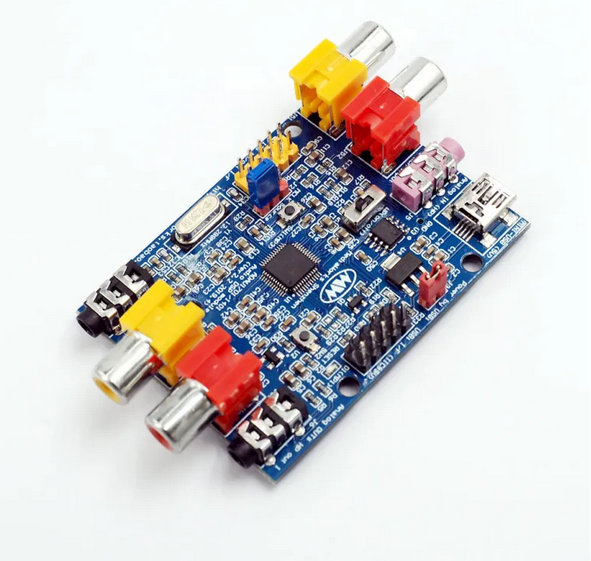
\includegraphics[height=5cm]{../fig/fig_ActiveControl/ADAU1701}};}
		\caption{}
		\label{fig:ActiveControl_ADAU1701}
	\end{subfigure}		
	\begin{subfigure}{.47\textwidth}
		\centering
		\external{fig_ActiveControl_Teensy41}
		\tikz{\draw(0,0) node{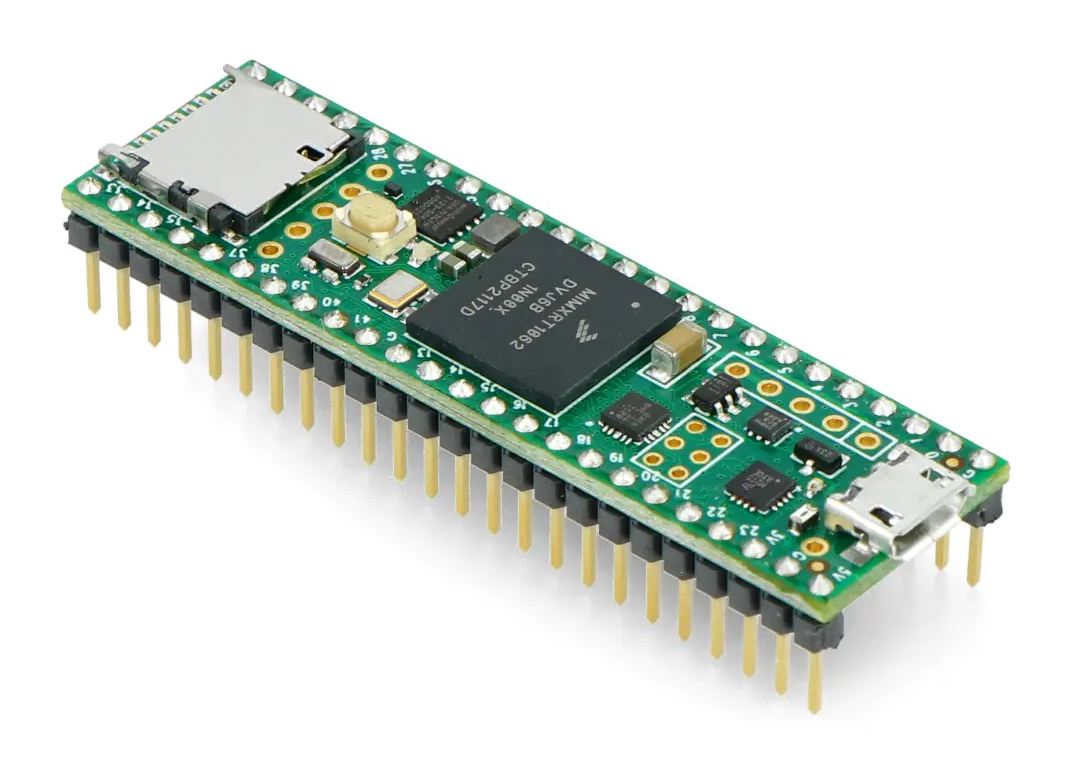
\includegraphics[height=5cm]{../fig/fig_ActiveControl/Teensy41}};}
		\caption{}
		\label{fig:ActiveControl_Teensy41}
	\end{subfigure}	    
    \caption{Dispositif de traitement du signal numérique en temps réel. \subref{fig:ActiveControl_ADAU1701} SigmaDSP ADAU1701 et \subref{fig:ActiveControl_Teensy41} Teensy 4.1}
    \label{fig:ActiveControl}
\end{figure}

Ces cartes sont toutefois sources de retards : les différents calculs réalisés par le processeur, les filtres, les conversions analogique-numérique et numérique-analogique prennent du temps, mais il est possible d'atteindre des retards faibles de l'ordre de \qty{80}{\micro\second}, ce qui correspond à un déphasage de \ang{1.35} à la fréquence de fonctionnement du \textsc{Tacot}, \qty{47}{\hertz}. Cette faible valeur rend possible leur utilisation pour un contrôle du champ acoustique dans la cavité thermoacoustique.

\subsection{Remplacement des sources acoustiques}
\subsubsection{Source principale}
La source acoustique principale est un moteur linéaire. Ce type de source est à la fois onéreux et difficile à se procurer, c'est pourquoi il peut être intéressant d'étudier l'impact sur les performances d'une source alternative. En l'occurrence un haut-parleur du commerce Ciare CSW7012EVO. 

\subsubsection{Source secondaire}





%---------------------------------------------------------------------%
% APPENDICES
%---------------------------------------------------------------------%
\newpage
\setcounter{page}{1}
\renewcommand{\thepage}{\alph{page}}
\appendix


\chapter{Index des notations}\label{chap:IndexNotations}%\addcontentsline{toc}{chapter}{\nameref{chap:IndexNotations}}

\textcolor{red}{Taille de la 2\ieme{} colonne pour remplir la page + reparcourir manuscript pour vérifier que c'est complet et cohérent}

\begin{center}
    \begin{tabular}{p{.15\textwidth} p{.75\textwidth}}
%    	\hline
        \multicolumn{2}{c}{Lettres latines}  \\\hline
        \textbf{Symbole} & \textbf{Définition} \\\hline\hline
        $\mathbf{g}$ & Constante de gravité, $\mathbf{g}=\qty{9.81}{\meter\per\second\squared}$ \\
        $g$ & Gain thermoacoustique \\
        $\Grashof$ & Nombre de Grashof \\
        $k_0$ & Nombre d'onde sans perte \\
        $c$ & Célérité du son dans le milieu \\
        $k$ & Conductivité thermique \\
        $K_p$ & Perméabilité hydraulique d'un matériau poreux \\
        $C_p$ & Capacité calorifique du gaz à pression constante \\
        $C_s$ & Capacité calorifique du solide poreux \\
        $C_v$ & Capacité calorifique du gaz à volume constant \\
        $L_{\sf reg}$ & Longueur du régénérateur, $L_{\sf reg}=\qty{39}{\milli\meter}$ \\
        $\Nusselt$ & Nombre de Nusselt \\
        $p_0$ & Pression statique dans le réfrigérateur \\
        $p$ & Pression acoustique \\
        $\Peclet$ & Nombre de Péclet \\
        $\Prandtl$ & Nombre de Prandtl \\
        $\mathbf{e}_r$ & Coordonnée radiale dans le noyau \\
        $R_{\sf reg}$ & Rayon du régénérateur, $R_{\sf reg}=\qty{74}{\milli\meter}$ \\
        $\Rayleigh$ & Nombre de Rayleigh \\
        $r_h$ & Rayon hydraulique des pores du régénérateur \\
        $T_0$ & Température moyenne locale du gaz dans le noyau \\
        $T_\infty$ & Température ambiante hors \textcolor{red}{du noyau / de la machine} \\
        $u$ & Débit acoustique \\
        $v$ & Vitesse acoustique \\
        $\mathbf{e}_x$ & Coordonnée axiale dans le noyau \\
        $Q_c$ & Flux de chaleur extrait par l'eau circulant dans l'échangeur ambiant \\
        $Q_f$ & Flux de chaleur apporté par les résistances chauffantes dans l'échangeur froid\\\hline
    \end{tabular}
\end{center}

\newpage

\begin{center}
    \begin{tabular}{p{.15\textwidth} p{.75\textwidth}}
%    	\hline
        \multicolumn{2}{c}{Lettres grecques \textcolor{red}{ordre alphabétique ?}}  \\\hline
        \textbf{Symbole} & \textbf{Définition} \\\hline\hline
        $\psi_v$ & Rotation de l'axe de symétrie du réfrigérateur par rapport à l'axe horizontal\\
        $\psi_h$ & Rotation autour de l'axe de symétrie du réfrigérateur \\
        $\varphi_{2-1}$ & Déphasage entre les sources acoustiques, $\varphi_{1-2} = \varphi_2 - \varphi_1$\\
        $\Phi$ & Porosité du régénérateur \\
        $\rho_0$ & Masse volumique moyenne du gaz \\
        $\rho_{s}$ & Masse volumique du solide poreux\\
        $\delta_{\kappa,\nu}$ & Couche limites thermique/visqueuse \\
        $\theta$ & Différence entre les températures locale dans le réfrigérateur et initiale, $\theta=T_0-T_\infty$\\
        $\mu$ & Viscosité dynamique \\
        $\nu$ & Viscosité cinématique \\
        $\kappa$ & Diffusivité thermique \\
        $\tau_0$ & Période du signal $\tau_0 = 1/f_0$ \\
        $\xi_0$ & Déplacement particulaire dans le régénérateur \\
        $\xi_1$ & Déplacement du piston de la source acoustique principale \\
        $\xi_2$ & Déplacement du piston de la source acoustique secondaire \\\hline
    \end{tabular}
\end{center}

\bigskip

\begin{center}
    \begin{tabular}{p{.15\textwidth} p{.75\textwidth}}
%		\hline
		\multicolumn{2}{c}{Indices et exposants}  \\\hline
		\textbf{Symbole} & \textbf{Définition} \\\hline\hline
		$\bullet^{\perp \mathbf g}$ & Perpendiculaire à la gravité $\mathbf g$ \\
		$\bullet^{//~\mathbf g}$ & Parallèle à la gravité $\mathbf g$ \\
		$\bullet^*$ & Conjugué complexe\\
		$\bullet_p$ & Lié au matériau poreux\\		
		$\bullet_g$ & Relatif au gaz dans le matériau poreux\\
		$\bullet_s$ & Relatif au solide du matériau poreux\\
		\hline
	\end{tabular}
\end{center}

\chapter{Caractérisation de l'échangeur ambiant}\label{chap:AHX}
Cette partie concerne la mesure de la chaleur extraite par l'échangeur ambiant $\dot Q_a$. Cet échangeur en cuivre conçu durant le projet \textsc{Tacot} et représenté sur la figure~\ref{fig:AHXschema} contient un circuit de canaux dans lequel circule de l'eau dont le débit peut être contrôlé \cite{ANR_thermo-acoustic_2019, ramadan_design_2021}. Son rôle est de maintenir l'extrémité chaude du régénérateur à température ambiante pour éviter l'échauffement globale du réfrigérateur. 

\begin{figure}[!ht]
    \centering
    \external{fig_AHXSchema}
    %\externalremake
    \begin{tikzpicture}
\draw (0,0) node {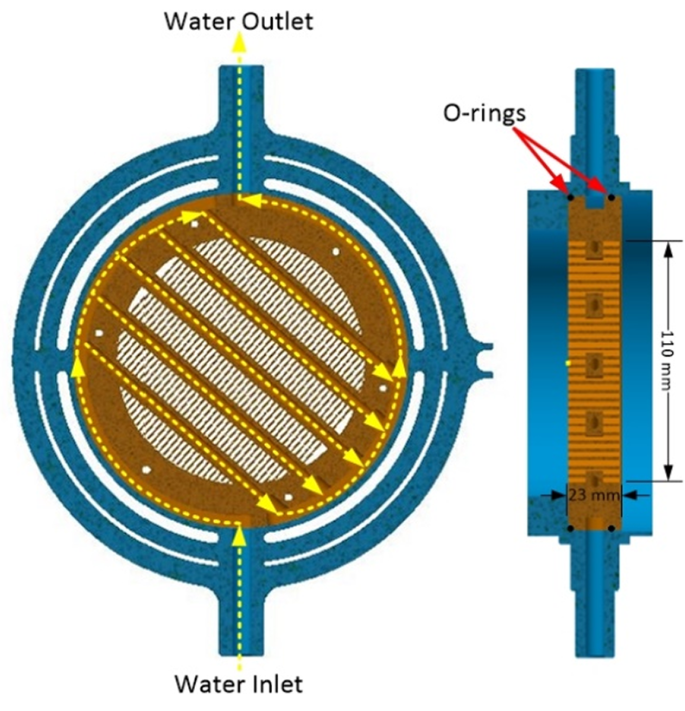
\includegraphics[width=.5\textwidth]{../fig/fig_AHXfromATE/AHXfromATE.png}};
    
\end{tikzpicture}
    \caption{Schéma de l'échangeur ambiant, issu de \cite{ramadan_design_2021}\echaf{ajouter TC \numlist{13;14;15} et le point de vue / axe $\mathbf e_x$}}
    \label{fig:AHXschema}
\end{figure}

Le but de cette étude est multiple : d'une part, l'alimentation en eau de l'échangeur se fait par un robinet puis est rejetée dans un évier, ce qui engendre un grand gaspillage. Son remplacement par un circuit fermé est prévu, mais il est nécessaire de connaître au préalable le débit nécessaire à un bon échange thermique. D'autre part, l'échange de chaleur dépend du débit d'eau $\dot q$ ainsi que de la différence de température de l'eau $\Delta T^w$ entre la sortie et l'entrée de l'échangeur. Cette dernière dépend également du débit, et le problème est donc de choisir le débit tel que la différence de température de l'eau soit la plus grande possible, tout en garantissant une extraction optimale de la chaleur par l'échangeur.

\section{Détermination de la chaleur pompée}
Tout d'abord, il est important de distinguer les flux de chaleur en jeu au niveau de l'échangeur ambiant. Le premier est celui qui transporte la chaleur de l'extrémité chaude du régénérateur à la partie solide l'échangeur ambiant, et le second, de cette partie solide de l'échangeur à l'eau qui y circule. Ils sont notés respectivement $Q_a'$ et $Q_a$, et c'est ce deuxième flux qu'il est possible d'estimer par la mesure de température d'eau.\smallskip

La quantité de chaleur extraite par l'eau à l'échangeur est définie par

\begin{equation}
    Q_a = m\ C_p\ \Delta T^w\quad,
    \label{eq:Qa_energie}
\end{equation}
où $m$ est la masse d'eau écoulée, $C_p$ la capacité calorifique de l'eau et $\Delta T^w$ la différence de température de l'eau entre l'entrée et la sortie de l'échangeur. La dérivée temporelle de cette équation donne la puissance thermique extraite par l'échangeur, qui s'écrit

\begin{equation}
    \dot Q_a = \dot m\ C_p\ \Delta T^w\quad,
    \label{eq:Qa_puissance}
\end{equation}

Pour prendre en compte l'écart intrinsèque aux capteurs de température, il est nécessaire de soustraire une différence $\Delta T_0^w$ qui correspond à l'écart de température de l'eau quand celle-ci circule dans l'échangeur, sans toutefois alimenter les sources acoustiques ni les charges thermiques\medskip

Les mesures de $\Delta T^w$ sont réalisées au moyen de sondes de platine PT100 pour les débits \qtylist{4.5;7;9.5}{\litre\per\minute} d'une eau à \qty{20}{\degreeCelsius}, et la chaleur extraite $\dot Q_a$ est déduite de ces mesures. Pour chaque débit, trois étapes sont réalisées : ouverture du robinet d'eau, puis démarrage des sources acoustiques, et enfin ajout d'une charge thermique $\dot Q_f$ du côté froid du régénérateur. Pour chacune de ces étapes, le régime transitoire ainsi que le régime établi sont acquis. Les résultats sont présentés figure~\ref{fig:AHXCalib} et représentent les quantités en régime établi. 

\begin{figure}[!ht]
    \centering
    \external{fig_AHXCalib}
%    \externalremake
    \begin{tikzpicture}
    \def\height{5cm};
    \def\width{.65\textwidth};
    \def\spx{1.2};
    \def\spy{.5cm};
    \def\legx{.5cm};
    \def\legy{.3cm};

    \begin{axis}[name=DTqdot,height=\height,width=\width, 
    x tick label style={
        /pgf/number format/1000 sep=},  
    %xlabel=$\dot q$ (\unit{\l\per\minute}),
    ylabel=$\Delta T^w$ (\unit{\degreeCelsius}),
    xmajorticks=false,
    ybar,enlarge x limits=.15,
    legend pos=outer north east]
    
    \addplot[solid,ultra thick,fill=MatlabBlue!25,draw=MatlabBlue] file {../fig/fig_AHXCalib/data/data_qdotDT0Water.txt};
    \addplot[solid,ultra thick,fill=MatlabOrange!25,draw=MatlabOrange,
    postaction={
        pattern=north east lines,pattern color=MatlabOrange
    }] file {../fig/fig_AHXCalib/data/data_qdotDT1WaterAcou.txt};
    \addplot[solid,ultra thick,fill=MatlabOrange!25,draw=MatlabOrange] file {../fig/fig_AHXCalib/data/data_qdotDT10Acou.txt};
    \addplot[solid,ultra thick,fill=MatlabYellow!25,draw=MatlabYellow,
     postaction={
        pattern=north east lines,pattern color=MatlabYellow
    }] file {../fig/fig_AHXCalib/data/data_qdotDT2WaterAcouQc.txt};
    \addplot[solid,ultra thick,fill=MatlabYellow!25,draw=MatlabYellow] file {../fig/fig_AHXCalib/data/data_qdotDT20AcouQc.txt};
    \legend{$\Delta T_0^w$ \\ $\Delta T_1^w$ \\ $\Delta T_1^w-\Delta T_0^w$ \\ $\Delta T_2^w$ \\ $\Delta T_2^w-\Delta T_0^w$ \\};
\end{axis}

\begin{axis}[name=Qdotqdot,height=\height,width=\width, 
    x tick label style={
        /pgf/number format/1000 sep=},  
    xlabel=$\dot q$ (\unit{\l\per\minute}),
    ylabel=$\dot Q_a$ (\unit{\watt}),
    xtick={4.5,7,9.5},
    ybar,enlarge x limits=.15,
    at={($(DTqdot.south)+(0,-\spy)$)},anchor=north,
    legend pos=outer north east]
    
    \addplot[solid,ultra thick,fill=MatlabOrange!25,draw=MatlabOrange] file{../fig/fig_AHXCalib/data/data_qdotQa1dotNoHeat.txt};
    \addplot[solid,ultra thick,fill=MatlabYellow!25,draw=MatlabYellow] file{../fig/fig_AHXCalib/data/data_qdotQa2dotHeat.txt};
    \legend{$\dot Q_f=0$ \\ $\dot Q_f \neq 0$ \\};
    \end{axis}
    
    \draw ($(DTqdot.north west)+(\legx,-\legy)$) node[]{\bf(a)};
    \draw ($(Qdotqdot.north west)+(\legx,-\legy)$) node[]{\textbf{(b)}};
\end{tikzpicture}
    \caption[Calibration de l'échangeur de chaleur ambiant.]{Calibration de l'échangeur de chaleur ambiant. \textbf{(a)} différence de température pour l'eau seule ($\Delta T_0^w$), après ajout des sources acoustiques en marche ($\Delta T_1^w$), puis après ajout d'une charge thermique $\dot Q_f$ ($\Delta T_2^w$). \textbf{(b)} puissance thermique $\dot Q_a$ extraite par l'eau en l'absence puis en présence d'une charge thermique $\dot Q_f$ côté froid.}
    \label{fig:AHXCalib}
\end{figure}




\section{Incertitudes de mesures}


\subsection{Température}
\echaf{blablabla}

\subsection{Débit d'eau}

La mesure du débit d'eau circulant dans l'échangeur ambiant est également source d'incertitude. En effet, le débitmètre à turbine utilisé \echaf{Marque, modèle} s'écarte de la valeur vraie du débit quand celui-ci est faible. Pour estimer l'écart à la réalité, la mesure par le débitmètre à turbine est comparé à celle par un débimètre à ultrason \echaf{vraiment le meilleur ? pourquoi ne pas utiliser l'ultrason pour toutes les manips ? pour la "valeur vraie", pourquoi pas un volume d'eau connu et un chrono ?}

\begin{figure}[!ht]
    \centering
    \external{fig_IncertitudeDebitEau}
%    \externalremake
    \begin{tikzpicture}
    \def\height{.9*\textwidth};
    \def\width{\height};
    \def\spx{.5cm};
    \def\spy{.5cm};
    \def\legx{.5cm};
    \def\legy{\legx};
    \def\prop{.45};
    
    \begin{axis}[name=TurbineUltrason,width={\width},height={\height},
    xlabel={$\dot q_{\textsf{us}}$ [\unit{\liter\per\minute}]},
    ylabel={$\dot q_{\textsf{tb}}$ [\unit{\liter\per\minute}]},
    xmin=0,xmax=10,ymin=0,ymax=10,
    domain=0:9.5,
    legend style = {at={(.97,.03)},anchor = south east}
    ]
        \addplot[solid,ultra thick,draw=MatlabBlue] file {../fig/fig_IncertitudeDebitEau/data/data_calibTurbineVSUltrason.txt} ;\addlegendentry{Exp.}
        \addplot[dashed,ultra thick,draw=MatlabBlue] {1.002*x - .3847}; \addlegendentry{Approx. linéaire,}
        \addlegendimage{empty legend}
        \addlegendentry{$\dot q_{\sf tb}=\dot q_{\sf us}-0.3847$}
        
%        \legend{Exp. \\ \begin{tabular}{l}Approx. linéaire\\$\dot q_{\sf tb}=\dot q_{\sf us}-0.3847$\end{tabular} \\};
    \end{axis}
    
    \begin{axis}[name=EcartRelat,width={\prop*\width},height={\prop*\height},
    xlabel={$\dot q$ [\unit{\liter\per\minute}]},
    ylabel={\'Ecart relatif $\epsilon$ [\unit{\percent}]},
    xmin=0,xmax=10,ymin=0,ymax=100,
    at={($(TurbineUltrason.north)+(\spx,-\spy)$)},anchor= north east
    ]
        \addplot[solid,ultra thick,draw=MatlabOrange] file {../fig/fig_IncertitudeDebitEau/data/data_RelativeDiff.txt};
    \end{axis}
    
    \draw ($(TurbineUltrason.north east)+(-\legx,-\legy)$) node[]{\bf (a)};
    \draw ($(EcartRelat.north east)+(-\legx,-\legy)$) node[]{\bf (b)};
    
\end{tikzpicture}
    \caption[Incertitudes de mesure du débit d'eau dans l'échangeur ambiant]{Incertitudes de mesure du débit d'eau dans l'échangeur ambiant. \textbf{(a)} débit mesuré par le débitmètre à turbine $\dot q_{\sf tb}$ en fonction de celui mesuré par le débitmètre à ultrason $\dot q_{\sf us}$. \textbf{(b)} écart relatif $\epsilon=\frac{|\dot q_{\sf us}-\dot q_{\sf tb}|}{\dot q_{\sf us}}$ entre les deux mesures obtenues.}
    \label{fig:IncertitudeDebitEau}
\end{figure}%

\echaf{Texte après le float}

\chapter{Instrumentation de la source secondaire}\label{chap:InstrumHP}
\section{But de l'opération}
Le déphasage des sources est un critère primordial pour l'obtention des meilleurs performances possibles avec cette machine. Au démarrage de la thèse, seule la source acoustique principale est munie d'un accéléromètre, et la phase de chaque source n'est réglée que sur le générateur basse fréquence utilisé. La source acoustique secondaire doit être instrumentée afin de connaître le déplacement de son piston au moyen d'un accéléromètre, sans pour autant perturber le système global en modifiant les paramètres électroacoustiques.

\section{Choix du capteur}


\section{Montage}
\begin{figure}[!ht]
    \centering
    \external{fig_HPPeerless_WithAcc}
    %\externalremake
    \tikz{\draw(0,0) node{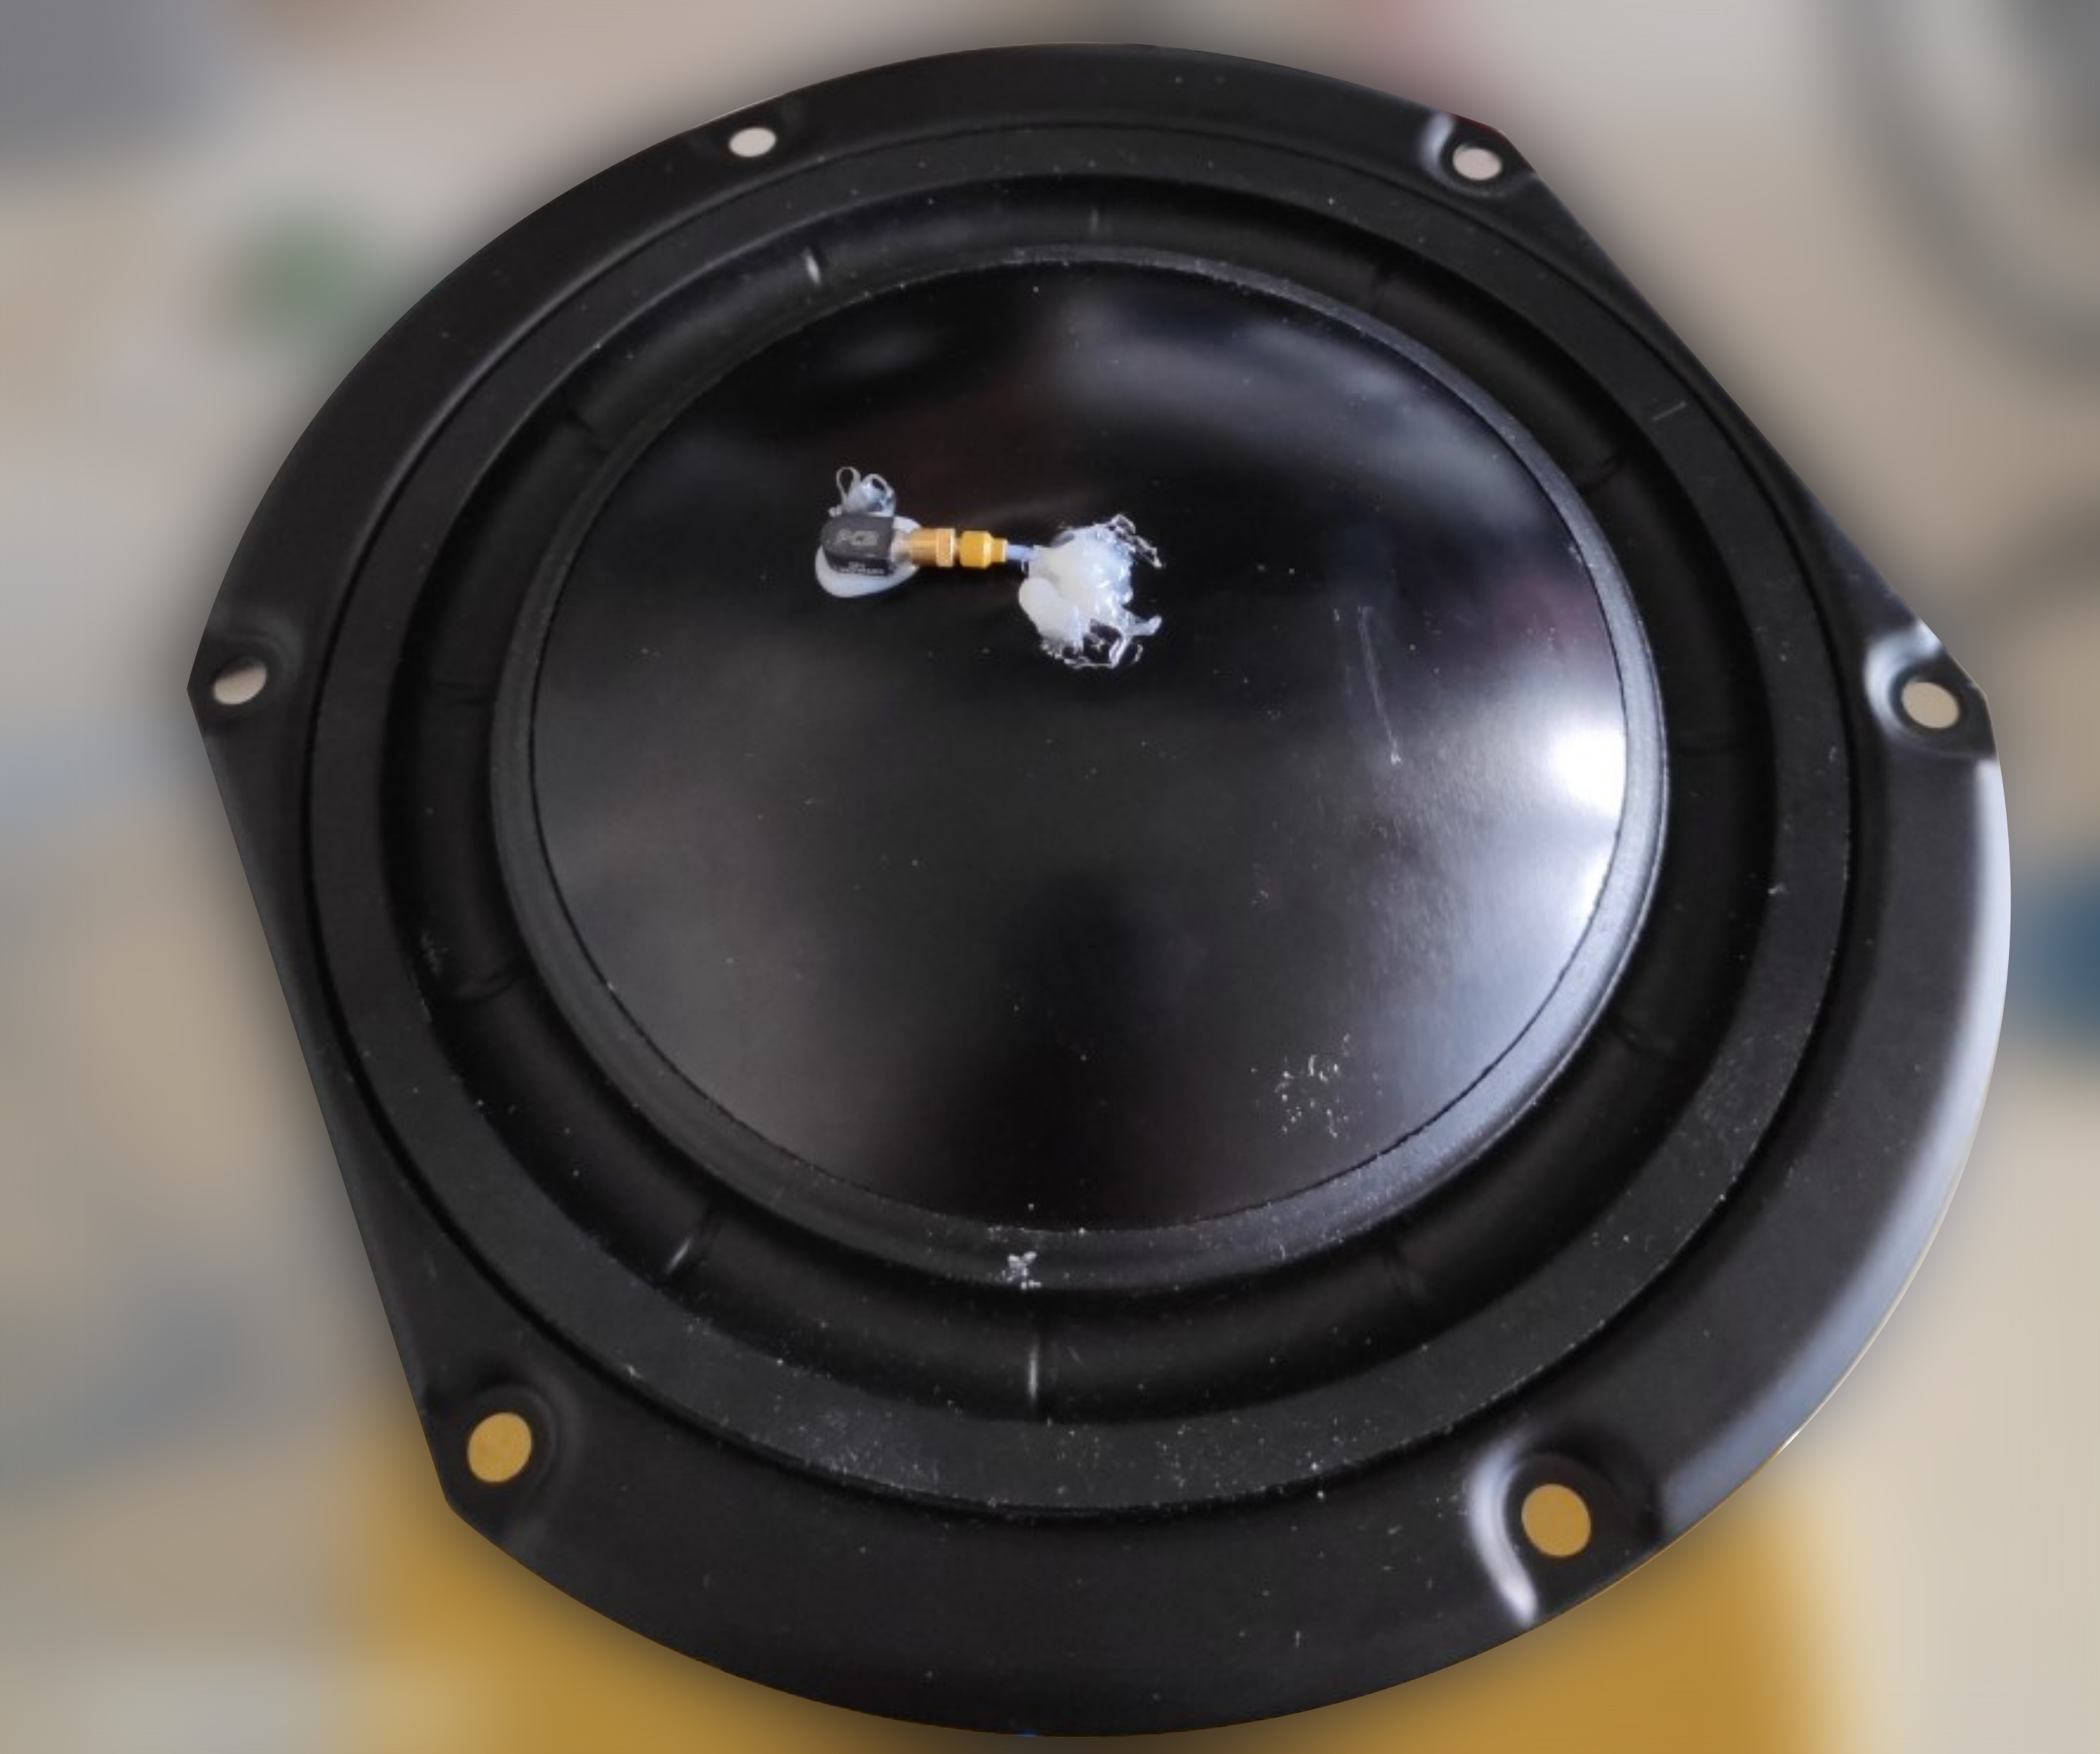
\includegraphics[width=.7\textwidth]{../fig/fig_InstrumentationHP/HPPeerless_WithAcc.png}};}
    \caption{Source acoustique secondaire avec l'accéléromètre collé sur sa membrane.}
    \label{fig:HPPeerless_WithAcc}
\end{figure}

\section{Vérification}
\subsection{Banc de mesures}

\subsection{Résultats}

\chapter{Paramètres du mélange de gaz choisi pour les expériences et simulations}\label{chap:ParamGaz}
\chaptermark{Paramètres du mélange de gaz utilisé}



\begin{table}[!ht]
	\centering
	\begin{tabular}{l @{\hspace{.5cm}} >{$} l <{$} @{\hspace{1cm}} l}
		\hline
		\textbf{Quantité} & \textbf{Symbole} &\textbf{Valeur}\\
		\hline\hline
		Masse volumique & \rho & ?\\
		Capacité calorifique & C_p &  ?\\
		Indice adiabatique & \gamma & ?\\
		Expansion thermique & \beta & ?\\
		Viscosité dynamique & \mu & ?\\
		Conductivité thermique & k & ?\\
		\hline
	\end{tabular}
	\caption{Résumé des paramètres thermodynamiques pour le mélange de gaz choisi.}
	\label{tab:ParamGaz}
\end{table}

\chapter{Récapitulatif des conditions expérimentales}
\section{\'Etude sur la convection naturelle}
Les conditions expérimentales du chapitre~\ref{chap:EtudeExpe_ConvNat} sont résumées de façon détaillée dans le tableau~\ref{tab:RecapCondExpe}.

\begin{longtable}{llll llll llll ll}
	\caption{Récapitulatif des conditions expérimentales.}
	\label{tab:RecapCondExpe}\\%
	
	\hline
	$\xi_1$ & $\xi_2$  & $DR$ & $p$ & $|Z_{ac}^{(1)}|$ & $|Z_{ac}^{(2)}|$& $\angle Z_{ac}^{(1)}$  & $\angle Z_{ac}^{(2)}$ & $T_a$  & $T_c$ & $\dot Q_a$ & $\dot Q_c$  & \multirow{2}{*}{Orientation} \\%
	
	\multicolumn{2}{c}{[\unit{\milli\meter}]} & [\unit{\percent}] & [\unit{\pascal}] & \multicolumn{2}{c}{[\unit{\pascal\second\per\meter}]} & \multicolumn{2}{c}{[\unit{\degree}]}  & \multicolumn{2}{c}{[\unit{\degreeCelsius}]} &\multicolumn{2}{c}{[\unit{\watt}]} &  \\\hline\hline \endfirsthead
	
	\hline
	$\xi_1$ & $\xi_2$  & $DR$ & $p$ & $|Z_{ac}^{(1)}|$ & $|Z_{ac}^{(2)}|$& $\angle Z_{ac}^{(1)}$  & $\angle Z_{ac}^{(2)}$ & $T_a$  & $T_c$ & $\dot Q_a$ & $\dot Q_c$  & \multirow{2}{*}{Orientation} \\%
	
	\multicolumn{2}{c}{[\unit{\milli\meter}]} & [\unit{\percent}] & [\unit{\pascal}] & \multicolumn{2}{c}{[\unit{\pascal\second\per\meter}]} & \multicolumn{2}{c}{[\unit{\degree}]}  & \multicolumn{2}{c}{[\unit{\degreeCelsius}]} &\multicolumn{2}{c}{[\unit{\watt}]} &  \\\hline\hline \endhead
	
	\hline
	\multicolumn{13}{r}{Continué sur la page suivante...} \endfoot
    \hline \endlastfoot
	
	0 & 0  &  \num{0} & 0 & -- & -- & -- & -- & \echaf{?} & \echaf{?} & \echaf{?} & 40 & \multirow{4}{*}{`\texttt{H1}'} \\*
	\echaf{?} & \echaf{?} &  \num{.4} & \echaf{?} & \echaf{?} & \echaf{?} & \echaf{?} & \echaf{?} & \echaf{?} & \echaf{?} & \echaf{?} & 0 &  \\*
	\echaf{?} & \echaf{?} &  \num{2} & \echaf{?} & \echaf{?} & \echaf{?} & \echaf{?} & \echaf{?} & \echaf{?} & \echaf{?} & \echaf{?} & 0 & \\*
	\echaf{?} & \echaf{?} &  \num{3.4} & \echaf{?} & \echaf{?} & \echaf{?} & \echaf{?} & \echaf{?} & \echaf{?} & \echaf{?} & \echaf{?} & 0 &  \\
	 \hdashline
	0 & 0 &  \num{0} & 0 & -- & -- & -- & -- &  &  &  & 40 & \multirow{4}{*}{`\texttt{H2}'} \\*
	 &  &  \num{.4} & & & &&& & \num{} & & 0 & \\*
	 &  &  \num{2} & & &&& & & \num{} & & 0 & \\*
	 &  &  \num{3.4} & & & &&& & \num{} & & 0 & \\
	 \hdashline
	0 & 0 &  \num{0} & 0 & -- & -- & -- & -- &  &  &  & 40 & \multirow{8}{*}{`\texttt{V1}'} \\*
	 &  &  \num{.4} & & & & &&& \num{} & & 0 & \\*
	 &  &  \num{2} &  & & &&& & \num{} & & 0 & \\*
	 &  &  \num{2} &  & & &&& & \num{} & & 50 & \\*
	 &  &  \num{2} &  & & &&& & \num{} & & 100 & \\*
	 &  &  \num{3.5} &  & & &&& & \num{} & & 0 & \\*
	 &  &  \num{3.5} &  & & &&& & \num{} & & 50 & \\*
	 &  &  \num{3.5} &  & & &&& & \num{} & & 100 & \\
	 \hdashline 
	0 & 0 &  \num{0} & 0 & -- & -- & -- & -- &  &  &  & 40 & \multirow{8}{*}{`\texttt{V2}'} \\*
	 &  &  \num{.4} & & && & && \num{} & & 0 & \\*
	 &  &  \num{2} & & & &&& & \num{} & & 0 & \\*
	 &  &  \num{2} & & & &&& & \num{} & & 50 & \\*
	 &  &  \num{2} & & & &&& & \num{} & & 100 & \\*
	 &  &  \num{3.5} &  & & & & \num{} & & & & 0 & \\*
	 &  &  \num{3.5} &  & & & & \num{} & & & & 50 & \\*
	 &  &  \num{3.5} &  & & & & \num{} & & & & 100 & \\*
\end{longtable}
	

\begin{table}[!ht]
	\caption{Récapitulatif des nombres adimensionnés.}
	\label{tab:RecapNbrAdim}
	\centering
	\begin{tabular}{>{$}l<{$} llll @{\hspace{25pt}} llll @{\hspace{25pt}} llll @{\hspace{25pt}} llll}\hline
	\multirow{2}{*}{\textbf{Nombre}} & \multicolumn{4}{c}{`\texttt{H1}'} & \multicolumn{4}{c}{`\texttt{H2}'} & \multicolumn{4}{c}{`\texttt{V1}'} & \multicolumn{4}{c}{`\texttt{V2}'}\\
	 & \num{0} & \num{.4} & \num{2} & \num{3.5} & \num{0} & \num{.4} & \num{2} & \num{3.5} & \num{0} & \num{.4} & \num{2} & \num{3.5} & \num{0} & \num{.4} & \num{2} & \num{3.5} \\ \hline\hline
	\Rayleigh &  &  &  &  &  &  &  &  &  &  &  &  &  &  &  &  \\
	\Peclet &  &  &  &  &  &  &  &  &  &  &  &  &  &  &  &  \\
	\Prandtl &  &  &  &  &  &  &  &  &  &  &  &  &  &  &  &  \\
	\Grashof &  &  &  &  &  &  &  &  &  &  &  &  &  &  &  &  \\
	\Nusselt &  &  &  &  &  &  &  &  &  &  &  &  &  &  &  &  \\ \hline
	\end{tabular}

\end{table}


\chapter{Fabrication d'un noyau thermoacoustique}
\mylocaltoc

\section{Quantité de tissus}
La porosité définie dans l'équation~\eqref{eq:Porosite_Volume} est modifiée et exprimée en fonction de la masse de tissus en acier inoxydable 316L à utiliser dans le montage comme

\begin{align}
	\Phi &= \frac{V_{\sf tot} - V_{\sf tis}}{V_{\sf tot}},\nonumber\\
		&= 1 - \frac{V_{\sf tis}}{V_{\sf tot}} = 1 - \frac{m_{\sf tis}}{m_{\sf tot}},\label{eq:Porisite_Masse}
\end{align}
ce qui permet d'introduire la masse de tissus en acier $m_{\sf tis}$ ainsi que la masse d'un cylindre de mêmes dimensions que le régénérateur entièrement constitué de ce métal.

\section{Instrumentation}

%\chapter{Circuit d'eau fermé pour l'échangeur ambiant}

Pour éviter la consommation excessive d'eau lors des campagnes de mesure, il est choisi d'assurer le maintien de la température de l'échangeur ambiant au moyen d'un circuit d'eau fermé. Ce circuit doit répondre à plusieurs critères :

\begin{enumerate}
    \item L'eau doit être stockée dans un reservoir dont le volume assure une augmentation de moins d'\qty{1}{\degreeCelsius} sur \qty{4}{\hour} de la température de l'eau ;\label{list:CircFerme_Volume}%
    \item le débit d'eau doit à la fois permettre d'extraire toute la chaleur à l'échangeur ambiant tout en réduisant les incertitudes de mesures liées aux capteurs de température de l'eau ;\label{list:CircFerme_Debit}%
    \item la pompe qui alimente le circuit doit \textcolor{red}{disposer/offrir} une charge suffisante pour compenser les pertes de charges régulière et singulières ainsi que la différence d'altitude entre l'échangeur et le reservoir d'eau.\label{list:CircFerme_Charge}
\end{enumerate}

\section{Débit}
La question du débit d'eau a été traitée dans l'annexe~\ref{chap:AHX}-\nameref{chap:AHX}, il est donc retenu un débit de $\qty{7}{\litre\per\minute}$

\section{Charges à fournir}
Pour choisir la pompe adaptée au circuit d'eau, 

\subsection{Différence de hauteur}
Le réservoir doit être disposé dans une pièce située sous le prototype du réfrigérateur. La hauteur à monter est de \qty{3}{\meter}.

\subsection{Régulières}
La connexion de l'échangeur au réservoir et à la pompe se fait par une trappe existante située à une dizaine de mètres du réfrigérateur. Pour évaluer les pertes de charge régulières causées par les tubes de raccordement, \qty{15}{\metre} de tube de diamètre 

\subsection{Singulières}


\section{Volume d'eau}


%\chapter{Changement des traversées}


%---------------------------------------------------------------------%
% BIBLIOGRAPHY
%---------------------------------------------------------------------%


\cleardoublepage

\setcounter{page}{1}

\renewcommand{\thepage}{\Roman{page}}

%\addcontentsline{toc}{chapter}{Bibliographie}

\setcounter{biburllcpenalty}{7000}
\setcounter{biburlucpenalty}{8000}
\printbibliography[title={Bibliographie}, heading=bibintoc]

\clearpage
\leavevmode

{
%\scriptsize

\vfill

{\Large Résumé :}\medskip

La thermoacoustique est un domaine interdisciplinaire à l'interface entre les transferts thermiques, la mécanique des fluides et l'acoustique. Elle concerne l'étude des interactions entre les ondes acoustiques et les variations de température. Dans cette thèse portant sur un réfrigérateur thermoacoustique, l'accent est mis sur l'impact de la convection naturelle sur la distribution de température complexe au sein de son noyau.

En effet, la convection naturelle est un phénomène où un transfert de chaleur et un mouvement de fluide est provoqué par des variations de densité causée par des différences de température. Cet écoulement et ces transferts thermiques peuvent influer sur les performances de la machine et  perturber la distribution de température déjà complexe dans un noyau thermoacoustique.

L'objectif principal de cette thèse expérimentale est d'analyser et de quantifier l'effet de la convection naturelle sur cette distribution de température. Une approche combinant simulations numériques et expérimentations est adoptée pour étudier les mécanismes sous-jacents régissant les transferts thermiques dans le noyau, en tournant le réfrigérateur et son noyau dans diverses orientations d'intérêt. Un modèle théorique temporel du régime transitoire est également développé pour prédire le comportement du système et ainsi améliorer la compréhension de la machine. Il est démontré que \echaf{ajouter les conclusions}.

Un espace dans la littérature portant sur la thermoacoustique est ainsi comblé par cette étude de l'impact de la convection naturelle sur la distribution de température dans le noyau du réfrigérateur thermoacoustique.

\bigskip

{\large \textit{Mots clés :}} thermoacoustique,  distribution de température, convection naturelle, conduction thermique, étude expérimentale, simulations numériques, modèles théoriques.

\vfill

{\Large Abstract:}\medskip

en Anglais

\bigskip

{\large \textit{Keywords:}} thermoacoustics, heat-driven/natural convection, temperature distribution

\vfill
}

%---------------------------------------------------------------------%
\end{document}
%---------------------------------------------------------------------%
